\documentclass[a4paper,12pt]{extarticle}
\usepackage[top=1in, bottom=1in, left=0.5in, right=0.5in]{geometry}
\usepackage[utf8]{inputenc}
\usepackage{caption,subcaption}
\usepackage{titlesec}
\usepackage{fancyhdr}
\usepackage[dvipsnames]{xcolor}
\usepackage[none]{hyphenat}
\usepackage{amsmath, amsfonts, amssymb, xfrac}
\usepackage{multicol}
\usepackage[super]{nth}
\usepackage{colortbl}
\usepackage{wasysym}
\usepackage{enumerate}
\usepackage{graphicx, epsfig, pgfplots}
\usepackage{float}
\usepackage{hyperref}
\usepackage{wrapfig}
\usepackage[table,xcdraw]{xcolor}
\usepackage{lipsum}
\definecolor{cblue}{HTML}{0F52BA}
\graphicspath{ {./images/} }

\pagestyle{fancy}
\fancyhf{}
\fancyhead[L]{Star Charts 101}
\fancyfoot[C]{\thepage}



\parindent 0ex
\title{{\fontsize{30}{30}\selectfont\blue{\textbf{Star Charts 101 and Practices}}}}
\author{Fahim Rajit Hossain}
\date{\today}


\begin{document}

\begin{titlepage}
	\maketitle
	
	
\begin{figure}[H]
    \centering
    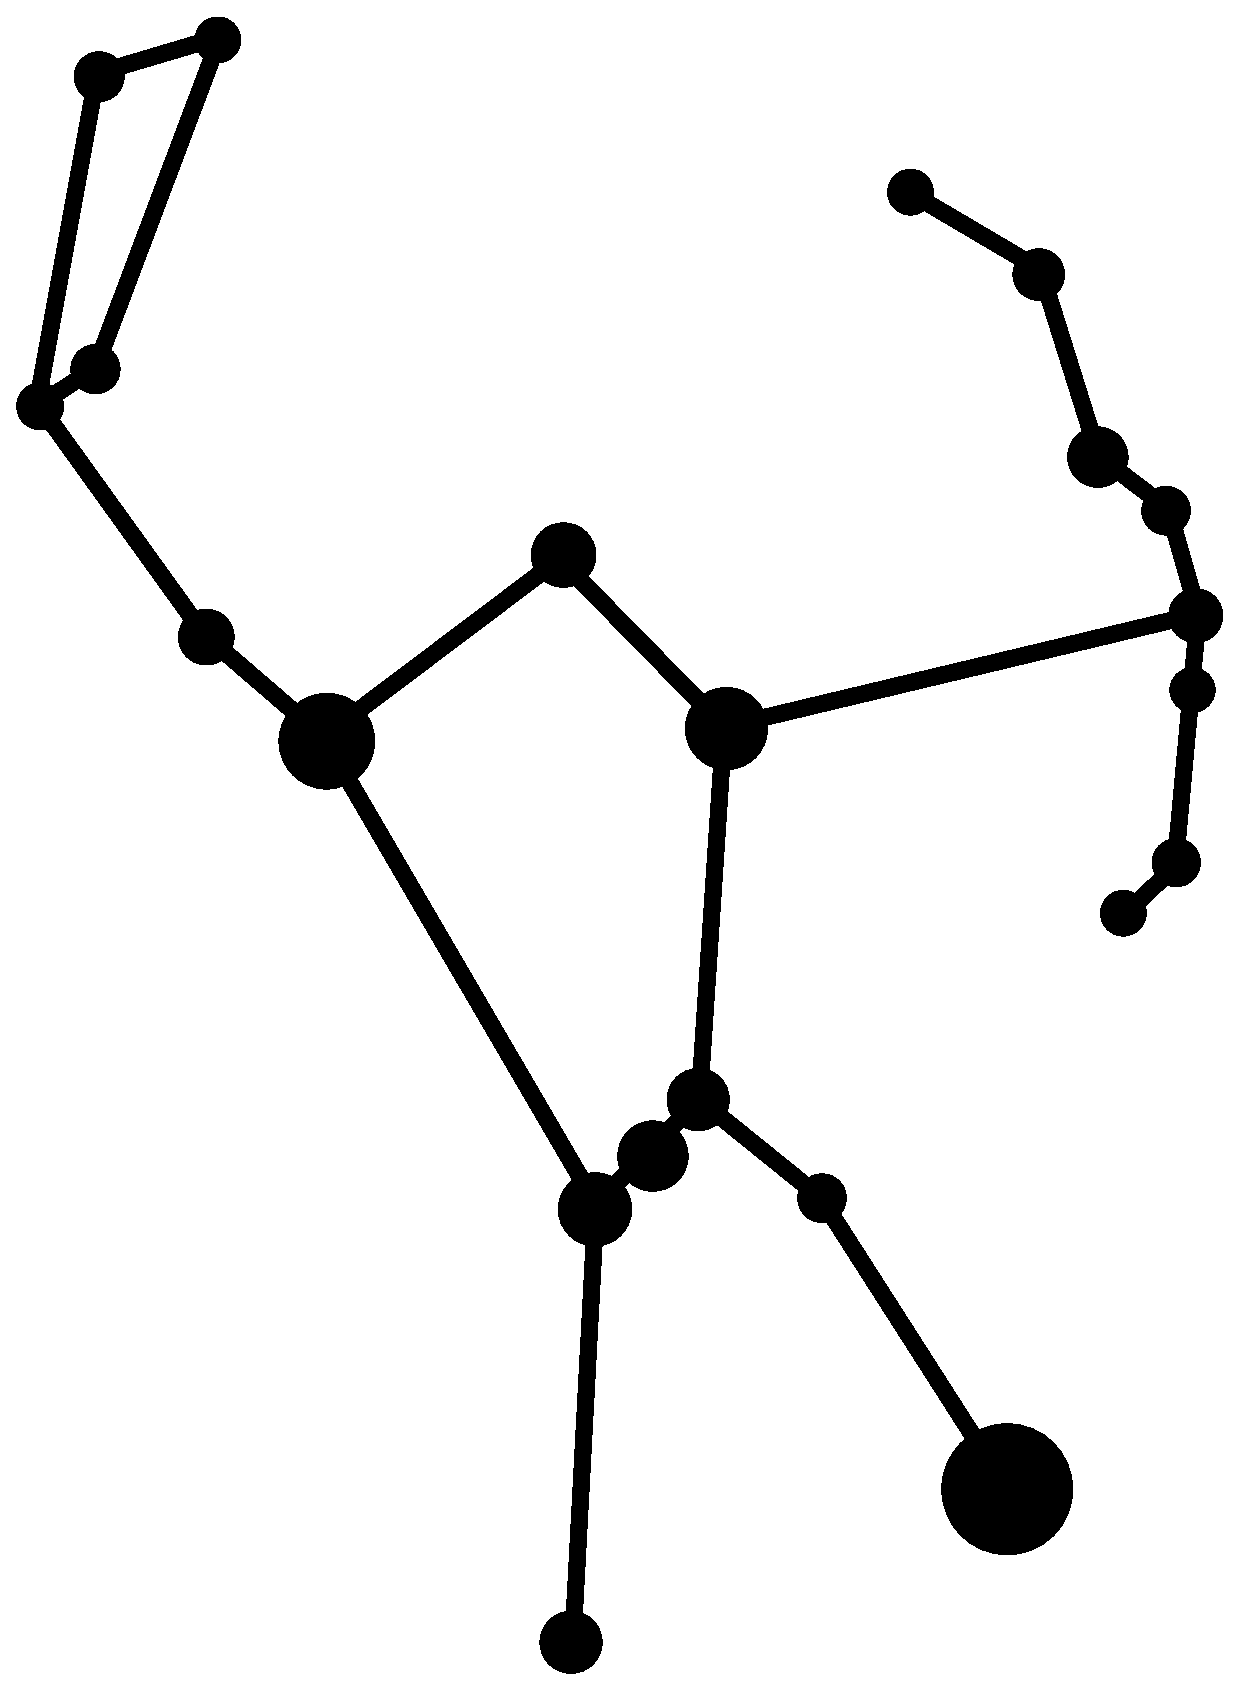
\includegraphics[width=0.35 \linewidth]{ori_1.eps}
\end{figure}
	
\vspace{1.5cm}
This practice book is dedicated to all Astronomy enthusiasts and those aiming for cracking Star Charts, part of Astronomy and Earth Science Olympiads. It is not a star atlas but it will fulfill its duty as a practice book. I'll recommend students to Print it and solve problems. \\

\textit{Written from my experience of both being a participant of two international Olympiads as well as team leader for IOAA since 2018. I've also tried to mix my added passion of stargazing into it! New versions can be found} -- \url{https://github.com/Rajit13/Star-Maps-101-and-Practices}

\vfill{\LaTeX  \;  compiled and  \copyright \; 2023 by \textsf{Fahim Rajit Hossain Shwadhin} is licensed under CC BY-NC-SA 4.0. To view a copy of this license, visit \url{http://creativecommons.org/licenses/by-nc-sa/4.0/} }\\

\hfill farahoshwadhin.13@gmail.com
\end{titlepage}

\tableofcontents

\clearpage
\begin{abstract}
	{\color{blue} This book delves into the fundamental knowledge necessary for computations associated with studying the sky and the positions of celestial objects, specifically in observational astronomy—focusing on naked-eye observation. It elucidates practical examples that progressively increase in complexity. Initially, memorizing all the constellations might seem daunting for enhanced observational skills. However, contrary to this belief, memorization isn't required. Instead, this book systematically guides you in understanding the sky, allowing you to approach challenges as if solving a puzzle.}
\end{abstract}
\section{Stars, Constellations, and Olympiads}
 
If you are aiming for Astronomy and Astrophysics Olympiad\footnote{IOAA/IAO} or even Earth Science Olympiad\footnote{IESO} you may find a portion  where problems contains a star map. So what is a star chart i.e. Sky Map?\\

But before that, you should know some basic concepts i.e what are Constellations? How stars move across the sky or it affects our observation? \\

\textbf{Constellations} represent apparent patterns formed by stars in the sky, often resembling figures or shapes perceived by humans. For instance, constellations might create recognizable figures like a Man (You may already guess the specific constellation I'm referring to!). They aid in identifying and recalling specific portions of the sky. However, it's important to note that creating random figures or personalized constellations is not officially recognized in Olympiads or by the International Astronomical Union (IAU). The IAU has officially acknowledged 88 constellations, while other popular patterns that are not part of these recognized constellations are referred to as Asterisms (e.g., Summer Triangle, Heavenly G, Big Dipper).\\

In a sky map, constellations are organized as their apparent orientation (projections) in the sky with respect to other celestial objects. In the Olympiads question setters provides a sky map of a certain region (latitude) and ask students to determine some things or identify objects or constellation. Basics of
Celestial Coordinate system is needed to understand the maps as well as solve the problems.

\subsection{Constellation Names}

Each Latin constellation name has two forms: the nominative, for use when talking about the constellation itself, and the genitive, or possessive, which is used in star names. For instance, Hamal, the brightest star in the constellation Aries (nominative form), is also called Alpha Arietis (genitive form), meaning literally, ``the alpha of Aries".\\

All modern constellations were codified in the European scientific subculture prior to the 19th century. As Latin was the international language of science up to that time, Latin governs the pronunciation of constellation names.\footnote{Source: \url{https://www.handprint.com/ASTRO/connames.html}} The Latin names of all the constellations, their abbreviated names and boundaries can be found in the table below. They are a mix of the ancient Greek patterns recorded by Ptolemy as well as some more ``modern" patterns observed later by more modern astronomers.\\

The IAU\footnote{Source: \url{https://www.iau.org/public/themes/constellations/}} adopted three-letter abbreviations of the constellation names at its inaugural General Assembly in Rome in 1922. The abbreviations devised by the IAU each have three letters which in the majority of cases are the first three letters of the constellation name, such as AND for Andromeda, EQU for Equuleus, HER for Hercules, ORI for Orion and so on. This trend is not strictly adhered to in cases where confusion may arise. This happens with the two constellations Leo (abbreviated LEO) and Leo Minor (abbreviated LMI). Similarly, because Triangulum (TRI) may be mistaken for Triangulum Australe, the latter is abbreviated TRA. Other instances occur with Sagitta (SGE) and Sagittarius (SGR) and with Canis Major (CMA) and Canis Minor (CMI) where the first two letters from the second names of the constellations are used. This is also the case with Corona Australis (CRA) and Corona Borealis (CRB) where the first letter of the second name of each constellation is incorporated. Finally, mention must be made of Crater (CRT) which has been abbreviated in such a way as to avoid confusion with the aforementioned CRA (Corona Australis).\\

In Olympiads, students are allowed to use star or constellation names based on their system, yet obtaining permission is necessary for IOAA/IAO/APAO competitions. Typically, team leaders should inquire about this with the host jury. Therefore, students from countries like Bangladesh are advised to consistently utilize names designated by the IAU. However, for a comprehensive understanding of the Bangla names of stars and constellations, along with their background stories, students are encouraged to read the book {\color{blue}``\textbf{Tara Porichity} by Abdul Jobbar''}.\\

\textbf{Learning how to recognize constellations}

\begin{enumerate}[1.]
	\item Write down the list of all the constellations you want to remember (let's call this to be ``C-List")
	\item Open the Stellarium app,
	\item Turn the constellation lines on, and the constellation names on.
	\item Find all the constellation from the ``C-list," try to remember where they are situated and how they look
	\item Turn the constellation names off (leave only the constellation lines on).
	\item Try to find all the constellations from the ``C-List" without the ``Search" function. If you can find the constellation, you strike it out of the ``C-list." If not, find it with the ``Search" function, try to remember where it is situated and how it looks.
	\item Then, repeat all the previous steps with all the constellations left after the first striking-out. If you can find the constellation you strike it out of the ``C-list". If not, find it with the "Search" function, try to remember where it is situated and how it looks
	\item Repeat the striking-out rounds until you have no constellations left in your ``C-list."
	\item If you every day repeat steps 1-8 (each day you start with blank ``C-list" with no constellations struck out), just in 4-5 days you will be able to recognize the constellations lines and will have the basic knowledge about how they are situated on the night sky.
	\item When you can strike all the constellations from the ``C-list" in one striking out round, you can start repeating all the previous steps, but now with constellation lines turned off. If you repeat these steps every day, just in some days you will get good skills of determining the position of the constellation, and recognizing it by its picture or stars around.
	
\end{enumerate}

\subsection{Star Names}

Most of the brighter stars were assigned their first systematic names by the German astronomer Johann Bayer in 1603, in his star atlas Uranometria . Bayer assigned a lowercase Greek letter, such as alpha ($\alpha$), beta ($\beta$), gamma ($\gamma$), etc., to each star he catalogued, combined with the Latin name of the star’s parent constellation in genitive (possessive) form. (See 88 modern constellations for the genitive forms later on the table.) For example, Aldebaran is designated $\alpha$ Tauri (pronounced Alpha Tauri), which means ``Alpha of the constellation Taurus".\\

A constellation’s most brilliant star is often called Alpha, the first letter in the Greek alphabet. The letters are used with the Latin genitive form of the constellation name, so the Alpha star of Centaurus is called “Alpha Centauri.” But there are few exceptions. For example, Gemini’s brightest star is $\beta$ and that of octans is $\nu$. Here is the lowercase Greek alphabet as used by astronomers:

\begin{table}[H]
\centering
\begin{tabular}{lll}
\begin{tabular}[c]{@{}l@{}}$\alpha$ Alpha\\ $\beta$ Beta\\ $\gamma$ Gamma\\ $\delta$ Delta\\ $\varepsilon$ Epsilon\\ $\zeta$ Zeta\\ $\eta$ Eta\\ $\theta$ Theta\end{tabular} & \begin{tabular}[c]{@{}l@{}}$\iota$ Iota\\ $\kappa$ Kappa\\ $\lambda$ Lambda\\ $\mu$ Mu\\ $\nu$ Nu\\ $\xi$ Xi\\ o Omicron\\ $\pi$ Pi\end{tabular} & \begin{tabular}[c]{@{}l@{}}$\rho$ Rho\\ $\sigma$ Sigma\\ $\tau$ Tau\\ $\upsilon$ Upsilon\\ $\phi$ Phi\\ $\chi$ Chi\\ $\Psi$ Psi\\ $\omega$ Omega\end{tabular}
\end{tabular}
\end{table}


In Olympiad questions, when asked about a star’s name examiners and Jury prefer these Greek letter titles (Flamsteed Designation or Bayer Designation) rather than actual
popular name. So it is a wise decision to remember star names by Greek letters.\\

A student should always know which star is the $\alpha$, $\beta$ star for a certain constellation. Specially
exceptions. Sometimes you may have to remember special stars designated $\gamma$ or $\zeta$ etc.\\

\textbf{Knowing where the brightest constellation stars are situated}\\

For learning where they are on the night sky, you can use the plan similar to the one for learning the constellations:
You can learn their position with the same plan

\begin{enumerate}[1.]
	\item  Write down the list of all the stars you want to remember (let's call this to be ``S-List")
	\item Open the Stellarium app, try to find a star without turning the names and lines of the constellations on. If you managed to strike it out of the ``S-List."
	\item If not, turn on the constellation lines and try to find the star again. If you managed to find it, leave the star in the list without striking it out.
	\item If not, find the star with the ``Search" function, try to remember where it is situated and how it looks. Don't strike it out.
	\item  Repeat the striking-out rounds until you have no stars left in your ``S-list."
\end{enumerate}

If you every day repeat steps 1-5 (each day you start with blank ``S-list" with no stars struck), just in a week, you will be able to recognize the stars on the night sky. You will also have a good knowledge of the relative positions of the constellations.




\clearpage
\begin{table}[H]
\caption{\textbf{Constellation Table}
}
\begin{tabular}{llclll}
\rowcolor[HTML]{EFEFEF} 
\multicolumn{1}{c}{\cellcolor[HTML]{EFEFEF}{\color[HTML]{000000} \textbf{No.}}} & {\color[HTML]{000000} \textbf{Constellation}} & {\color[HTML]{000000} \textbf{Location}} & {\color[HTML]{000000} \textbf{Supposed Figure}} & \multicolumn{1}{c}{\cellcolor[HTML]{EFEFEF}{\color[HTML]{000000} \textbf{Code}}} & {\color[HTML]{000000} \textbf{Brightest Star}} \\
1                                                                               & Andromeda                                     & N                                        & Andromeda                                       & And                                                                              & Alpheratz ($\alpha$)                           \\
2                                                                               & Antlia                                        & S                                        & The Air Pump                                    & Ant                                                                              & {\color[HTML]{000000} $\alpha$ Antliae}        \\
3                                                                               & Apus                                          & S                                        & The Bird of Paradise                            & Aps                                                                              & $\alpha$ Apodis                                \\
4                                                                               & Aquarius                                      & S/Eq                                     & The Water Carrier                               & Aqr                                                                              & Sadal Melik ($\alpha$)                         \\
5                                                                               & Aquila                                        & Eq                                       & The Eagle                                       & Aql                                                                              & Altair ($\alpha$)                              \\
6                                                                               & Ara                                           & S                                        & The Altar                                       & Ara                                                                              & $\beta$ Arae                                   \\
7                                                                               & Aries                                         & N                                        & The Ram                                         & Ari                                                                              & Hamal ($\alpha$)                               \\
8                                                                               & Auriga                                        & N                                        & The Charioteer                                  & Aur                                                                              & Capella ($\alpha \ast$)                        \\
9                                                                               & Boötes                                        & N                                        & The Herdsman                                    & Boo                                                                              & Arcturus  ($\alpha$)                           \\
10                                                                              & Caelum                                        & S                                        & The Graving Tool                                & Cae                                                                              & $\alpha$ Caeli                                 \\
11                                                                              & Camelopardalis                                & N                                        & The Giraffe                                     & Cam                                                                              & $\beta$ Camelopardalis                         \\
12                                                                              & Cancer                                        & N                                        & The Crab                                        & Cnc                                                                              & Al Tarf  ($\beta$)                             \\
13                                                                              & Canes Venatici                                & N                                        & The Hunting Dogs                                & CVn                                                                              & Cor Caroli ($\alpha$)                          \\
14                                                                              & Canis Major                                   & S                                        & The Great Dog                                   & CMa                                                                              & Sirius  ($\alpha \ast$)                        \\
15                                                                              & Canis Minor                                   & N/Eq                                     & The Little Dog                                  & CMi                                                                              & Procyon ($\alpha \ast$)                        \\
16                                                                              & Capricornus                                   & S                                        & The Goat                                        & Cap                                                                              & Al Giedi ($\alpha$)                            \\
17                                                                              & Carina                                        & S                                        & The Keel                                        & Car                                                                              & Canopus ($\alpha\ast$)                         \\
18                                                                              & Cassiopeia                                    & N                                        & Cassiopeia                                      & Cas                                                                              & Shedir ($\alpha$)                              \\
19                                                                              & Centaurus                                     & S                                        & The Centaur                                     & Cen                                                                              & Rigel Kentaurus  ($\alpha \ast$)               \\
20                                                                              & Cepheus                                       & S                                        & Cepheus                                         & Cep                                                                              & Alderamin  ($\alpha$)                          \\
21                                                                              & Cetus                                         & Eq                                       & The Whale                                       & Cet                                                                              & Diphda  ($\beta$)                              \\
22                                                                              & Chamaeleon                                    & S                                        & The Chameleon                                   & Cha                                                                              & $\alpha$ Chamaeleontis                         \\
23                                                                              & Circinus                                      & S                                        & The Pair of Compasses                           & Cir                                                                              & $\alpha$ Circini                               \\
24                                                                              & Columba                                       & S                                        & The Dove                                        & Col                                                                              & Phact ($\alpha$)                \\
25                                                                              & Coma Berenices                                & N                                        & Berenice’s Hair                                 & Com                                                                              & $\beta$ Comae Berenices                        \\
26                                                                              & Corona Australis                              & S                                        & The Southern Crown                              & CrA                                                                              & $\alpha$ Coronae Australis     \\
27 & Corona Borealis & N    & The Northern Crown     & CrB & Gemma or Alphecca ($\alpha$)       \\
28 & Corvus          & S    & The Crow               & Crv & Gienah ($\gamma$)                  \\
29 & Crater          & S    & The Cup                & Crt & $\delta$ Crateris                  \\
30 & Crux            & S    & The Cross              & Cru & Acrux ($\alpha \ast$)              \\
31 & Cygnus          & N    & The Swan               & Cyg & Deneb ($\alpha \ast$)              \\
32 & Delphinus       & N    & The Dolphin            & Del & Rotanev ($\beta$)                  \\
33 & Dorado          & S    & The Goldfish           & Dor & $\alpha$ Doradus                   \\
34 & Draco           & N    & The Dragon             & Dra & Etamin ($\gamma$)                  \\
35 & Equuleus        & N    & The Foal               & Equ & Kitalpha ($\alpha$) \\
36 & Eridanus        & S/Eq & The River              & Eri & Achernar ($\alpha \ast$)           \\
37 & Fornax          & S    & The Furnace            & For & $\alpha$ Fornacis                  \\
38 & Gemini          & N    & The Twins              & Gem & Pollux ($\beta \ast$)              \\
39 & Grus            & S    & The Crane              & Gru & Alnair ($\alpha$)                  \\
40 & Hercules        & N    & Hercules               & Her & Ras Algethi ($\alpha$)             \\
41 & Horologium      & S    & The Pendulum Clock     & Hor & $\alpha$ Horologii                 \\
42 & Hydra           & S/Eq & The Water Snake        & Hya & Alphard ($\alpha$)                 \\
43 & Hydrus          & S    & The Lesser Water Snake & Hyi & $\beta$ Hydri                      \\
44 & Indus           & S    & The Indian             & Ind & $\alpha$ Indi      
\end{tabular}
\end{table}

\clearpage



\begin{table}[H]
\begin{tabular}{llclll}
\rowcolor[HTML]{EFEFEF} 
{\color[HTML]{000000} \textbf{No.}} & {\color[HTML]{000000} \textbf{Constellation}} & {\color[HTML]{000000} \textbf{Location}} & {\color[HTML]{000000} \textbf{Supposed Figure}} & {\color[HTML]{000000} \textbf{Code}} & {\color[HTML]{000000} \textbf{Brightest Star}} \\
45 & Lacerta         & N    & The Lizard             & Lac & $\alpha$ Lacertae                  \\
46 & Leo             & N/Eq & The Lion               & Leo & Regulus ($\alpha \ast$)            \\
47 & Leo Minor       & N    & Lion Cub               & LMi & Praecipua  \\
48 & Lepus           & S    & The Hare               & Lep & Arneb ($\alpha$)                   \\
49 & Libra           & S    & The Scales             & Lib & Zubeneschamali ($\beta$)           \\
50 & Lupus           & S    & The Wolf               & Lup & $\alpha$ Lupus                     \\
51 & Lynx            & N    & The Lynx               & Lyn & $\alpha$ Lyncis                    \\
52 & Lyra            & N    & The Lyre               & Lyr & Vega ($\alpha \ast$)               \\
53 & Mensa           & S    & The Table Mountain     & Men & $\alpha$ Mensae                    \\
54 & Microscopium    & S    & The Microscope         & Mic & $\gamma$ Microscopii       \\
55                         & Monoceros                            & Eq                              & The Unicorn                            & Mon                         & $\beta$ Monocerotis                   \\
56                         & Musca                                & S                               & The Fly                                & Mus                         & $\alpha$ Muscae                       \\
57                         & Norma                                & S                               & The Level                              & Nor                         & $\gamma$ Normae                       \\
58                         & Octans                               & S                               & The Octant                             & Oct                         & $\nu$ Octanis                         \\
59                         & Ophiuchus                            & Eq                              & The Serpent Bearer                     & Oph                         & Ras Alhague ($\alpha$)                \\
60                         & Orion                                & Eq                              & The Hunter                             & Ori                         & Rigel ($\beta \ast$)                  \\
61                         & Pavo                                 & S                               & The Peacock                            & Pav                         & $\alpha$ Pavonis                      \\
62                         & Pegasus                              & N                               & Pegasus                                & Peg                         & Enif ($\varepsilon$)                  \\
63                         & Perseus                              & N                               & Perseus- Demi God                      & Per                         & Mirfak ($\alpha$)                     \\
64                         & Phoenix                              & S                               & The Phoenix                            & Phe                         & Ankaa ($\alpha$)                      \\
65                         & Pictor                               & S                               & The Painter’s Easel                    & Pic                         & $\alpha$ Pictoris                     \\
66                         & Pisces                               & N/Eq                            & The Fish                               & Psc                         & $\eta$ Piscium                        \\
67                         & Pisces Australis                     & S                               & The Southern Fish                      & PsA                         & Fomalhaut ($\alpha\ast$)              \\
68                         & Puppis                               & S                               & The Stern                              & Pup                         & Naos ($\zeta$)                        \\
69                         & Pyxis                                & S                               & The Mariner’s Compass                  & Pyx                         & $\alpha$ Pyxidis                      \\
70                         & Reticulum                            & S                               & The Net                                & Ret                         & $\alpha$ Reticuli                     \\
71                         & Sagitta                              & S                               & The Arrow                              & Sge                         & $\gamma$ Sagittae                     \\
72                         & Sagittarius                          & S                               & The Archer                             & Sgr                         & Kaus Australis ($\varepsilon$)        \\
73                         & Scorpius                             & S                               & The Scorpion                           & Sco                         & Antares ($\alpha \ast$)               \\
74                         & Sculptor                             & S                               & The Sculptor                           & Scl                         & $\alpha$ Sculptoris                   \\
75                         & Scutum                               & S                               & The Shield                             & Sct                         & Ionnina                               \\
76                         & Serpens                              & Eq                              & The Serpent                            & Ser                         & Unukalhai ($\alpha$)                  \\
77                         & Sextans                              & Eq                              & The Sextant                            & Sex                         & $\alpha$ Sextantis                    \\
78                         & Taurus                               & N/Eq                            & The Bull                               & Tau                         & Aldebaran ($\alpha \ast$)             \\
79                         & Telescopium                          & S                               & The Telescope                          & Tel                         & $\alpha$ Telescopii                   \\
80                         & Triangulum                           & N                               & The Triangle                           & Tri                         & $\beta$ Trianguli                     \\
81                         & Triangulum Australe                  & S                               & The Southern Triangle                  & TrA                         & Atria ($\alpha$)  \\
82 & Tucana     & S  & The Toucan      & Tuc & $\alpha$ Tucanae       \\
83 & Ursa Major & N  & The Great Bear  & UMa & Alioth ($\varepsilon$) \\
84 & Ursa Minor & N  & The Little Bear & Umi & Polaris ($\alpha$)     \\
85 & Vela       & S  & The Sail        & Vel & Suhail ($\alpha$)      \\
86 & Virgo      & Eq & The Virgin      & Vir & Spica ($\alpha \ast$)  \\
87 & Volans     & S  & The Flying Fish & Vol & $\beta$ Volantis       \\
88 & Vulpecula  & N  & The Fox         & Vul & Anser 
\end{tabular}
\end{table}

\textbf{$^\ast$ Indicates brightest stars in the sky}

\begin{table}[H]
\centering
\begin{tabular}{lllllll}
$\alpha$ And                & $\beta$ Aur  & $\alpha$ CMa  & $\alpha$ Gem & $\alpha$ Ori & $\alpha$ Psc      & $\beta$ UMa   \\
$\beta$ And                 & $\alpha$ Boo & $\beta$ CMa   & $\beta$ Gem  & $\beta$ Ori  & $\alpha$ Sco      & $\alpha$ UMi \\
$\alpha$ Ari                & $\beta$ Boo  & $\alpha$ CMi  & $\alpha$ Leo & $\alpha$ Oph & $\beta$ Sco       & $\beta$ UMi  \\
$\beta$ Ari                 & $\alpha$ Cap & $\beta$ CMi   & $\beta$ Leo  & $\beta$ Oph  & $\alpha$ Ser      & $\beta$ Cyg  \\
$\alpha$ Aql                & $\alpha$ Cas & $\alpha$ CrB  & $\alpha$ Lep & $\alpha$ Per & $\varepsilon$ Sgr &              \\
$\beta$ Aql                 & $\beta$ Cas  & $\beta$ CrB   & $\alpha$ Lib & $\beta$ Per  & $\alpha$ Tau      &              \\
$\alpha$ Aqr                & $\alpha$ Cep & $\gamma$  Dra & $\alpha$ Lyr & $\alpha$ Peg & $\beta$ Tau       &              \\
$\alpha$ Aur & $\alpha$ Cet & $\alpha$ Cyg  & $\beta$ Lyr  & $\beta$ Peg  & $\alpha$ UMa      &             
\end{tabular}
\caption{Suggested Bright Stars of interest}
\end{table}

\textbf{List of brightest natural objects in the sky}- \url{https://en.wikipedia.org/wiki/List_of_brightest_natural_objects_in_the_sky}
\subsection{Constellation Figures}

In star maps it is common to mark line “patterns” that represent the shapes that give the name to the constellations. However, the IAU defines a constellation by its boundary (indicated by sky coordinates) and not by its pattern and the same constellation may have several variants in its representation.\\

The constellations should be differentiated from asterisms. Asterisms are patterns or shapes of stars that are not related to the known constellations, but nonetheless are widely recognized by laypeople or in the amateur astronomy community. Examples of asterisms include the seven bright stars in Ursa Major known as “the Plough” in Europe or “the Big Dipper” in America, as well as “the Summer Triangle”, a large triangle, seen in the summer night sky in the northern hemisphere and composed of the bright stars Altair, Deneb and Vega. Whilst a grouping of stars may be officially designated a constellation by the IAU, this does not mean that the stars in that constellation are necessarily grouped together in space. Sometimes stars will be physically close to each other, like the Pleiades, but constellations are generally really a matter of perspective. They are simply our Earth-based interpretation of two dimensional star patterns on the sky made up of stars of many differing brightnesses and distances from Earth.\\

In the next page you'll find the official figures from IAU. Notice that you should only remember constellation figures from IAU. You'll find many constellation shapes on the internet which might differ due to distortion or variable observation. 

\vfill{
\begin{figure}[H]
    \centering
    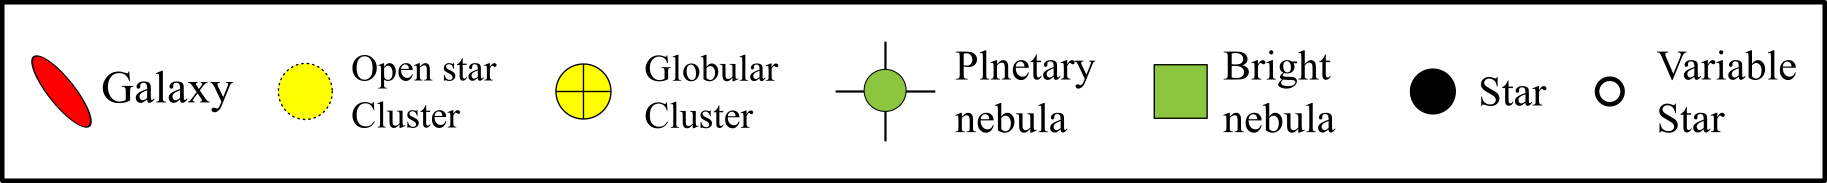
\includegraphics[width=0.8\linewidth]{legend.png}
\end{figure}}
\clearpage
\begin{figure}
    \centering
    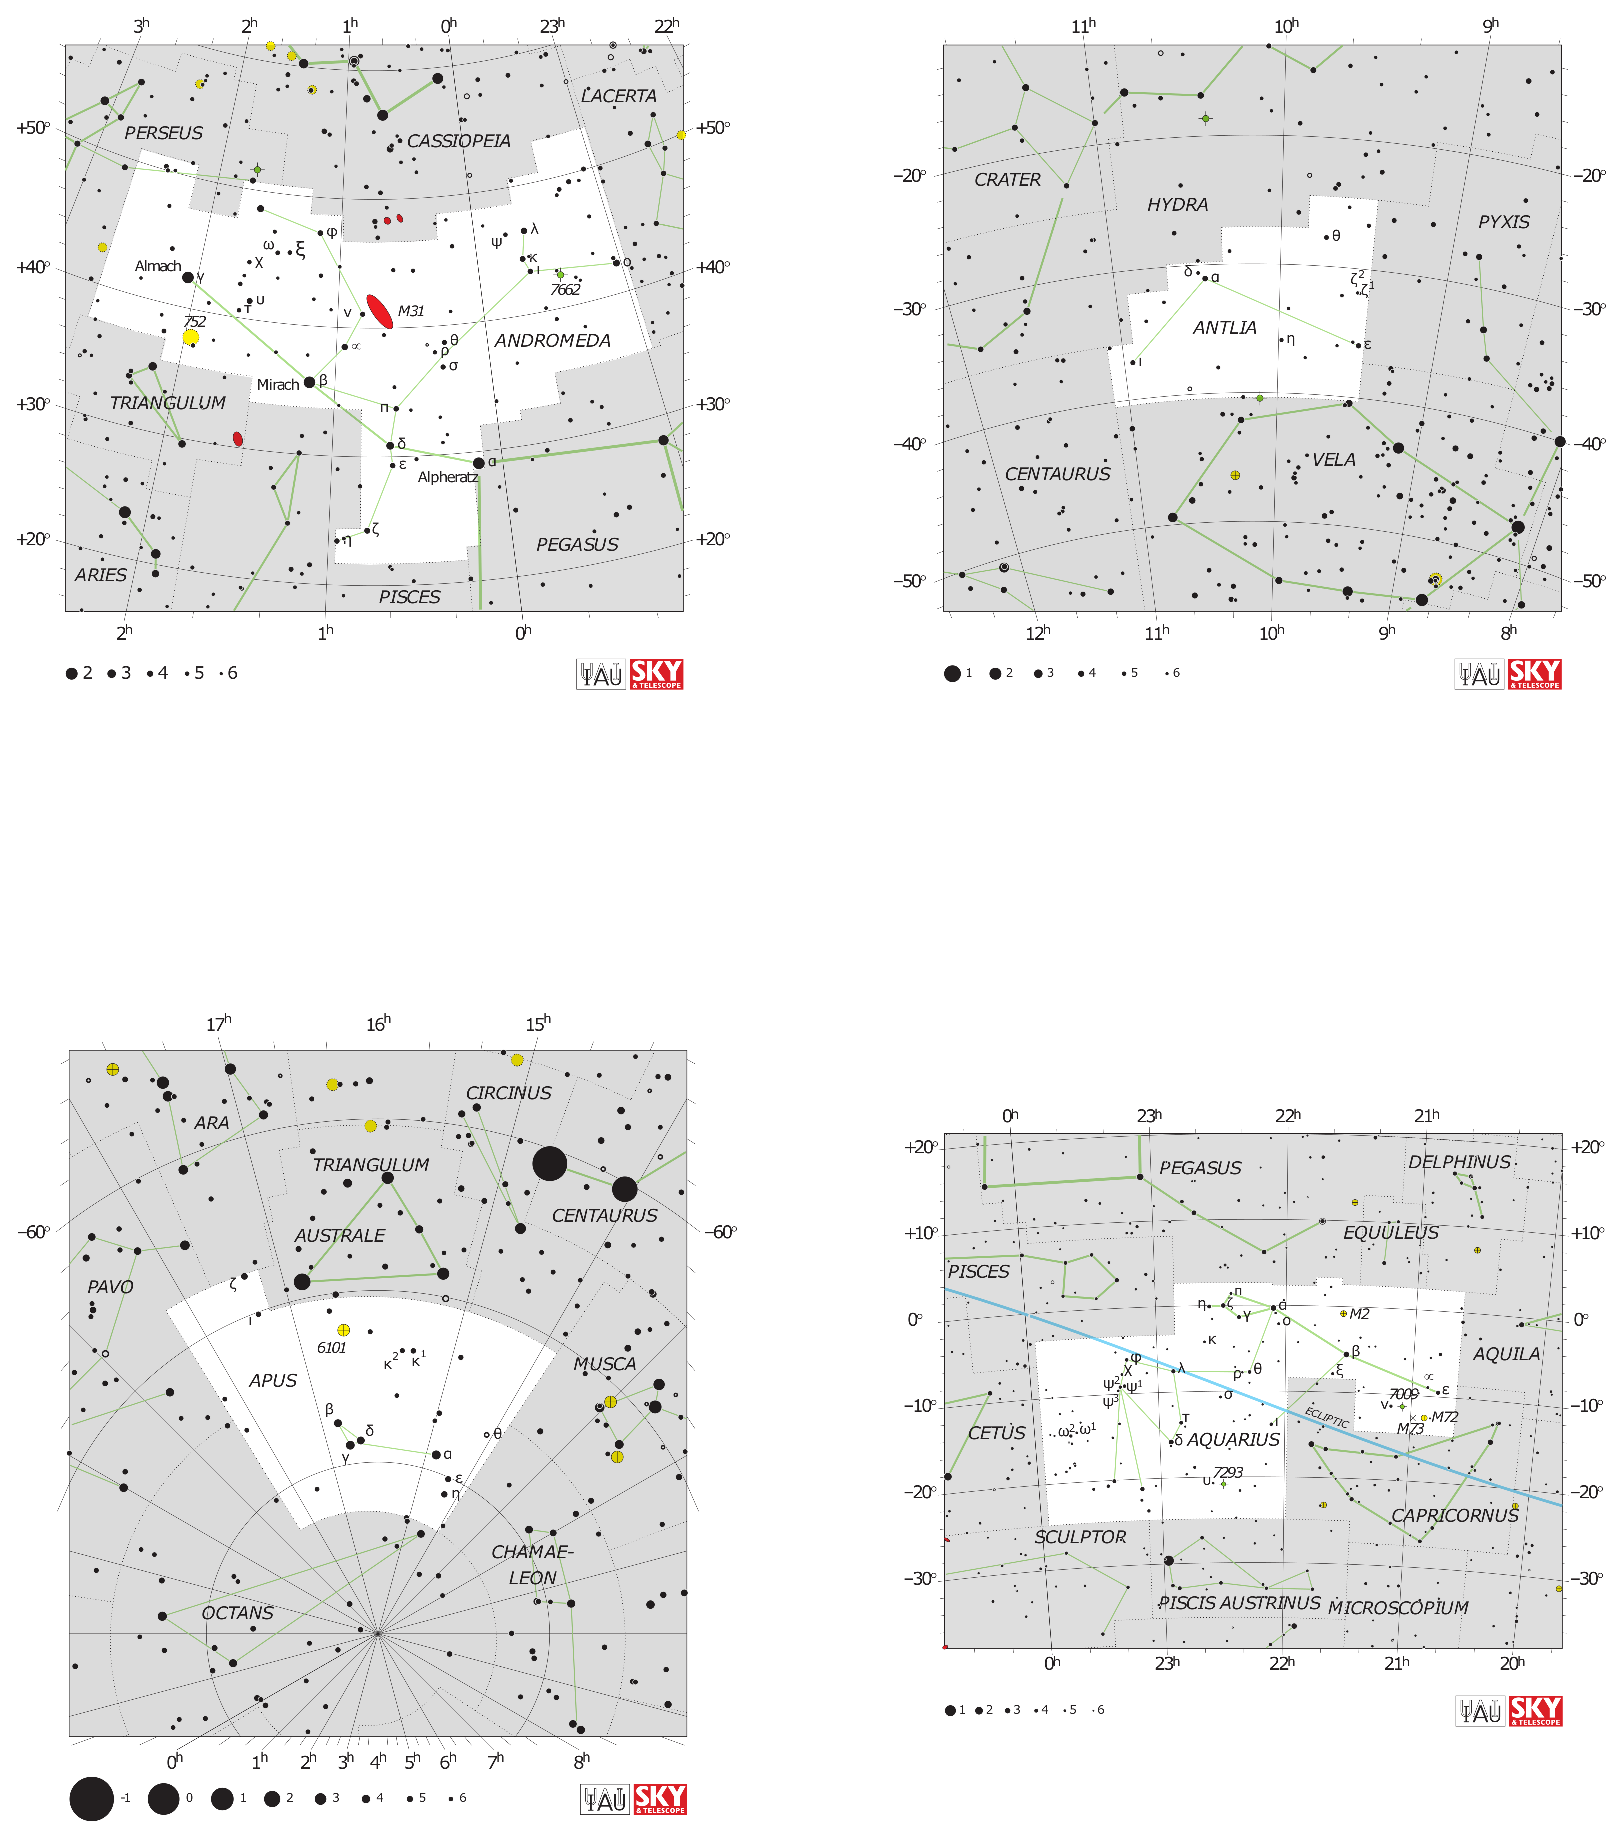
\includegraphics[width=\linewidth]{C1.eps}
\end{figure}
\clearpage
\begin{figure}
    \centering
    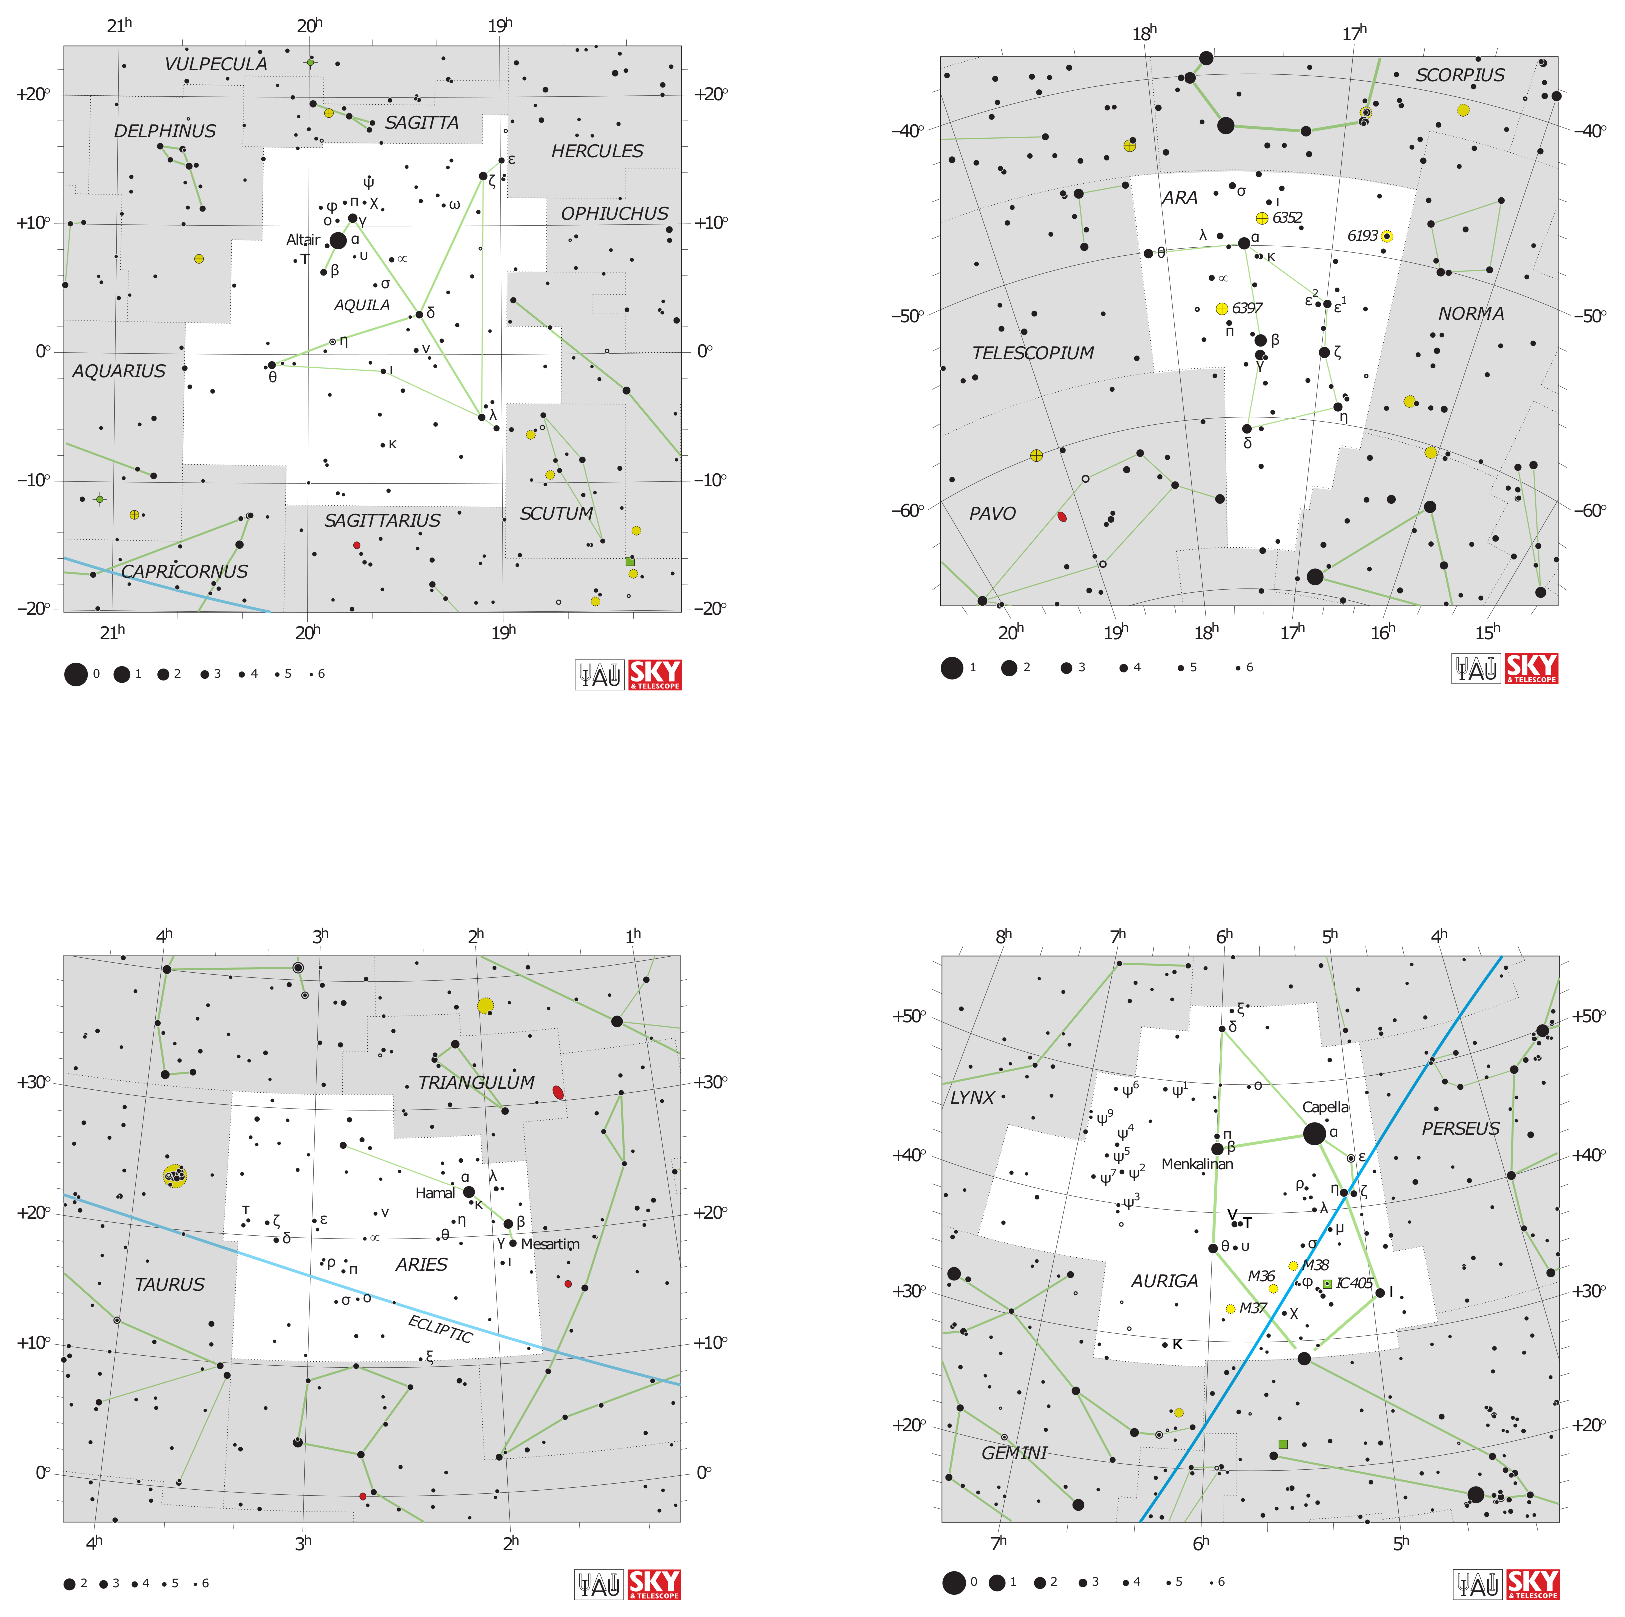
\includegraphics[width=\linewidth]{C2.eps}
\end{figure}

\clearpage
\begin{figure}
    \centering
    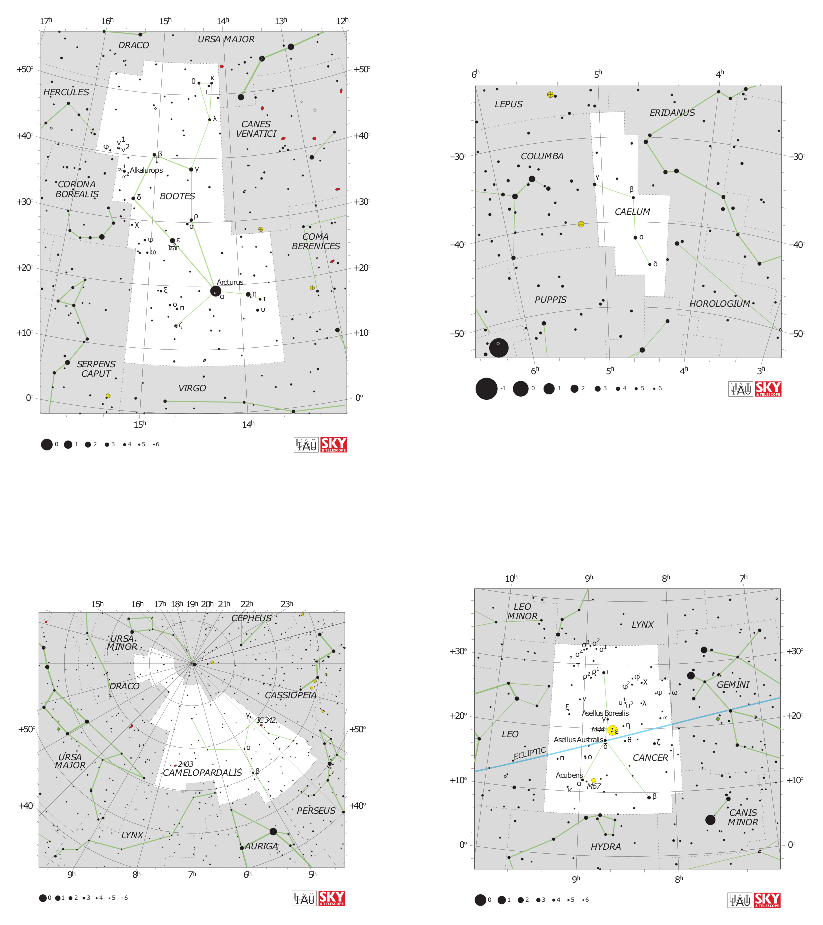
\includegraphics[width=\linewidth]{C3.eps}
\end{figure}
\clearpage
\begin{figure}
    \centering
    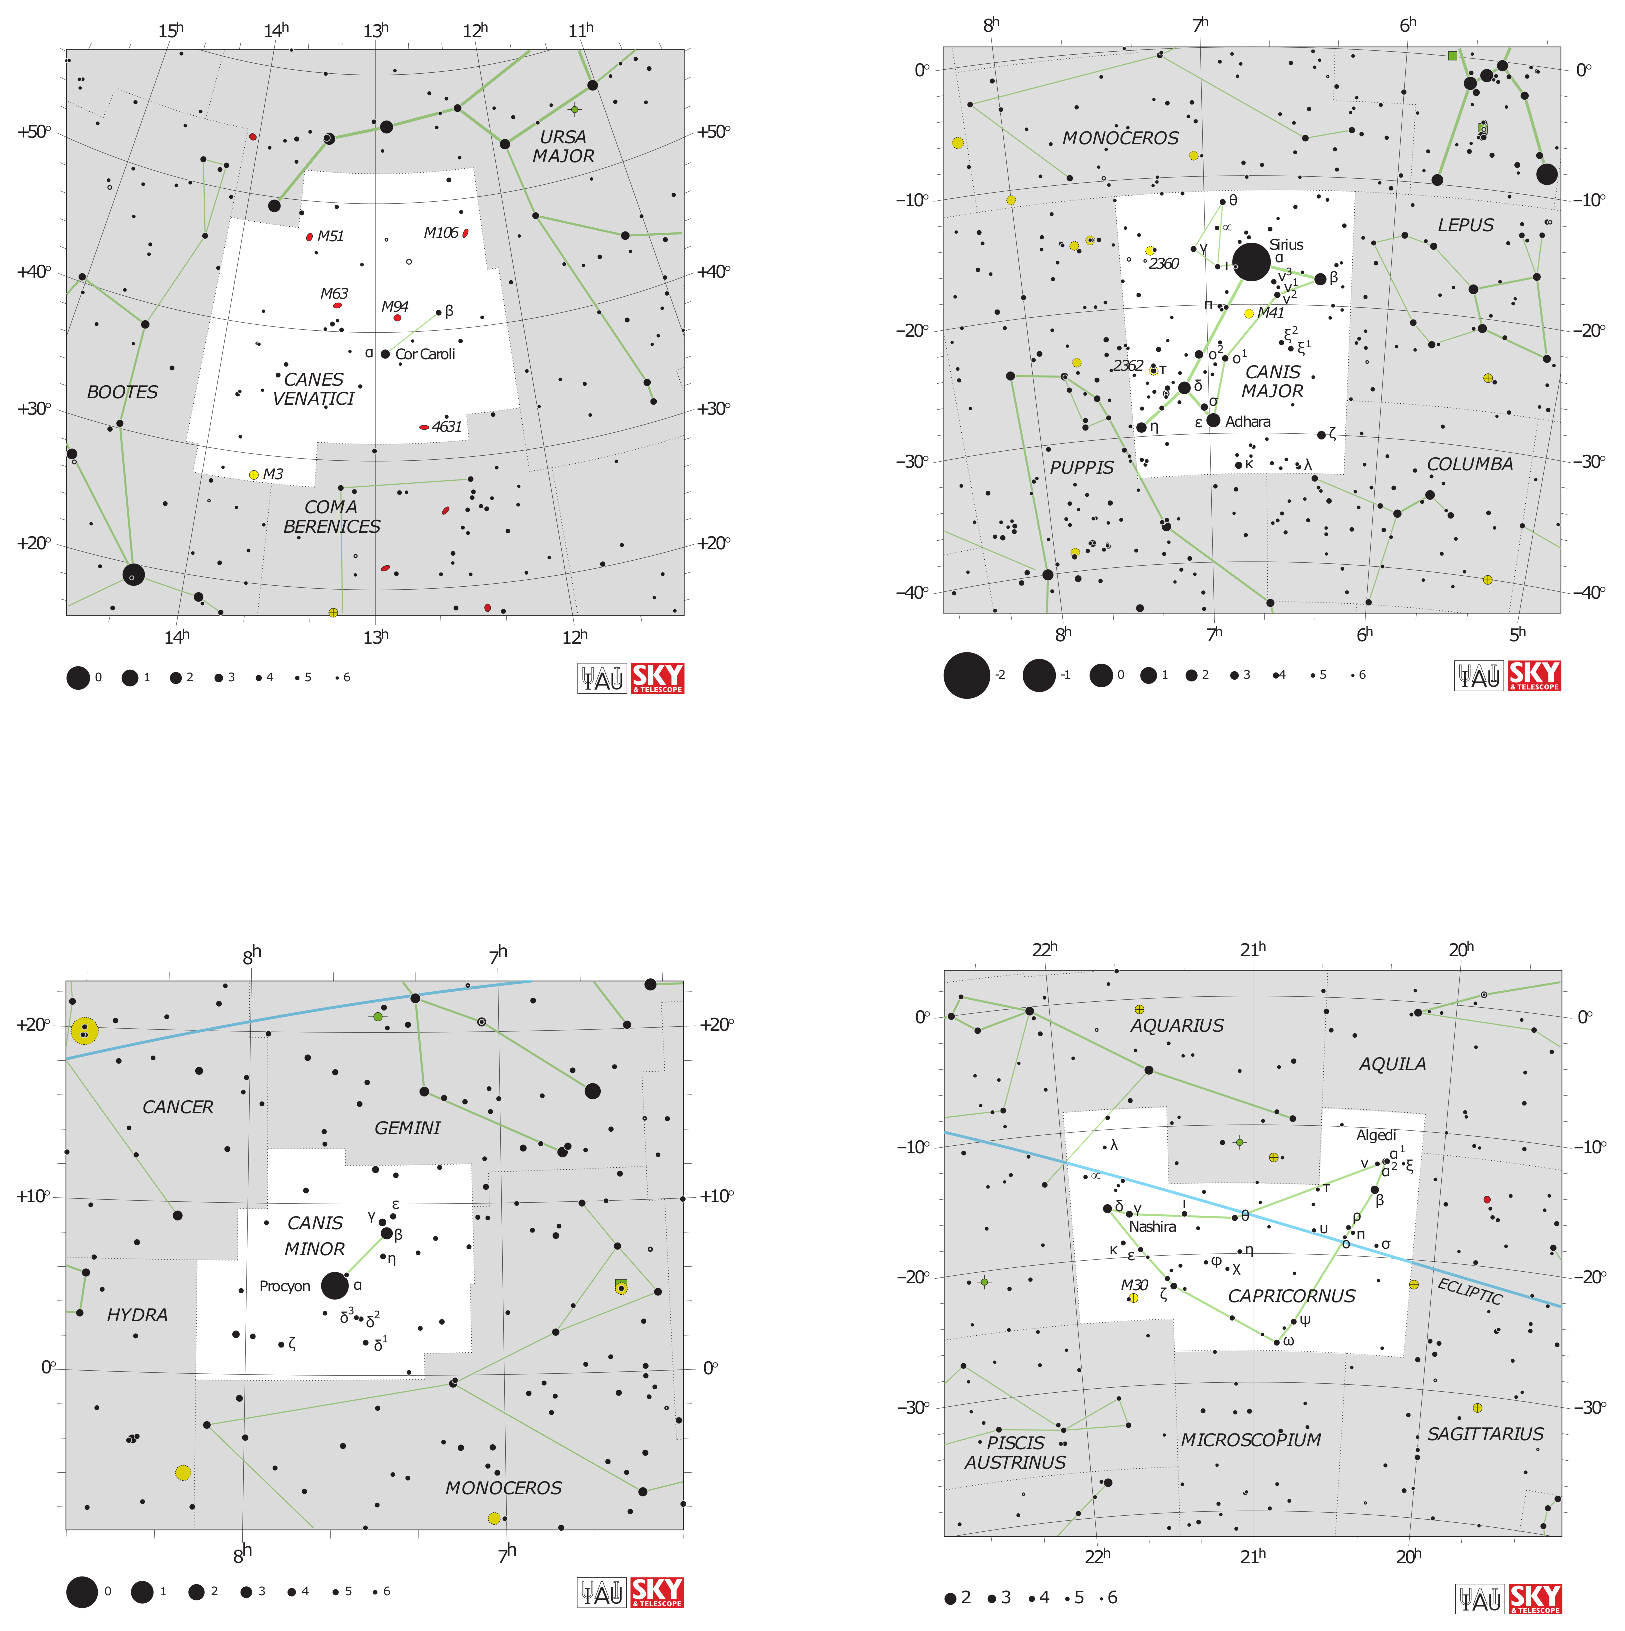
\includegraphics[width=\linewidth]{C4.eps}
\end{figure}
\clearpage
\begin{figure}
    \centering
    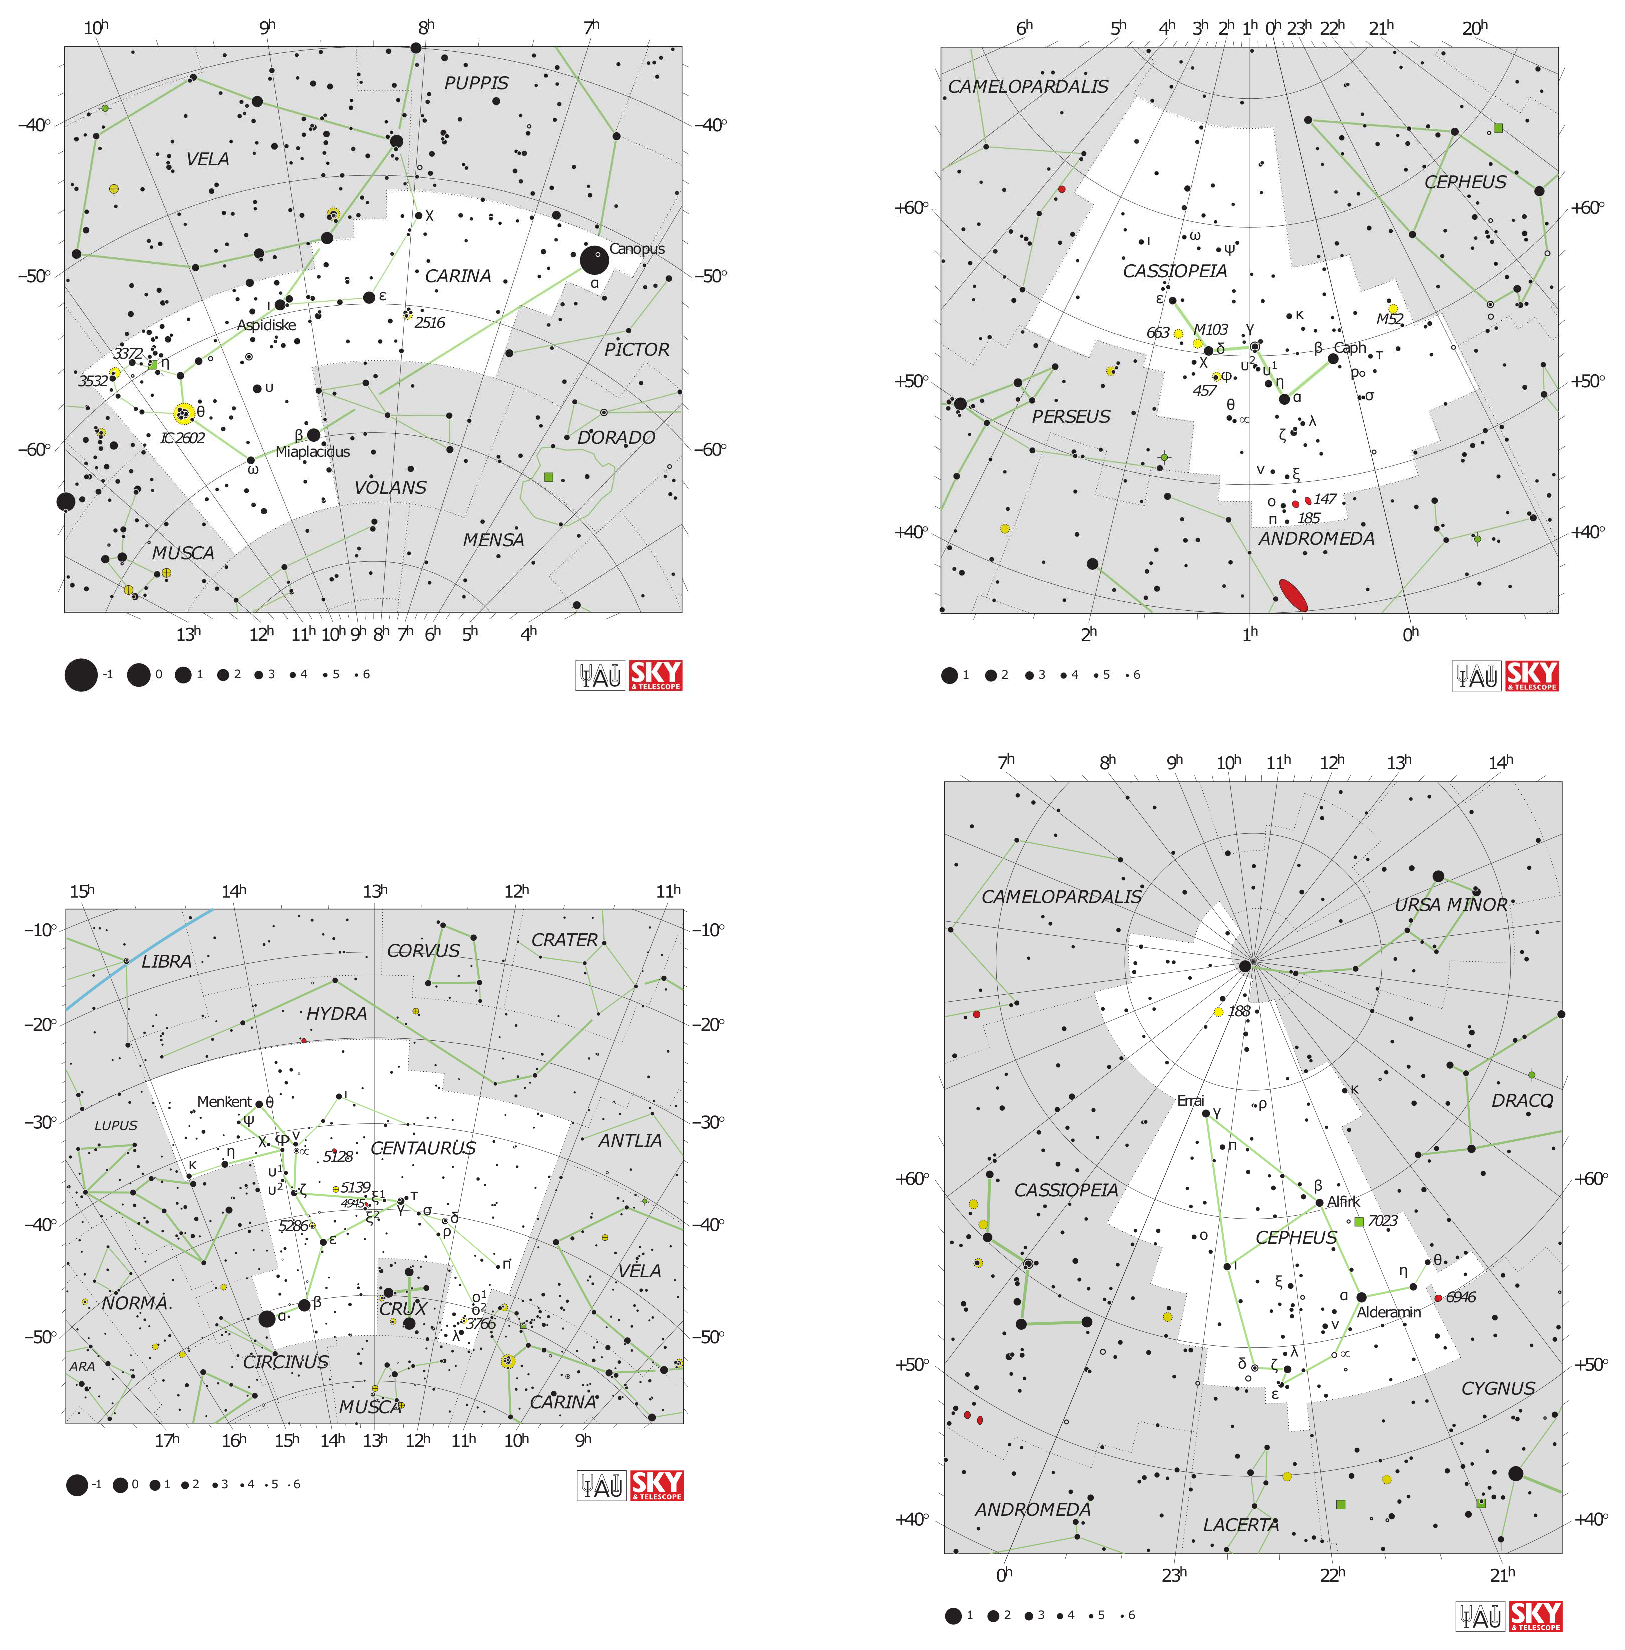
\includegraphics[width=\linewidth]{C5.eps}
\end{figure}
\clearpage
\begin{figure}
    \centering
    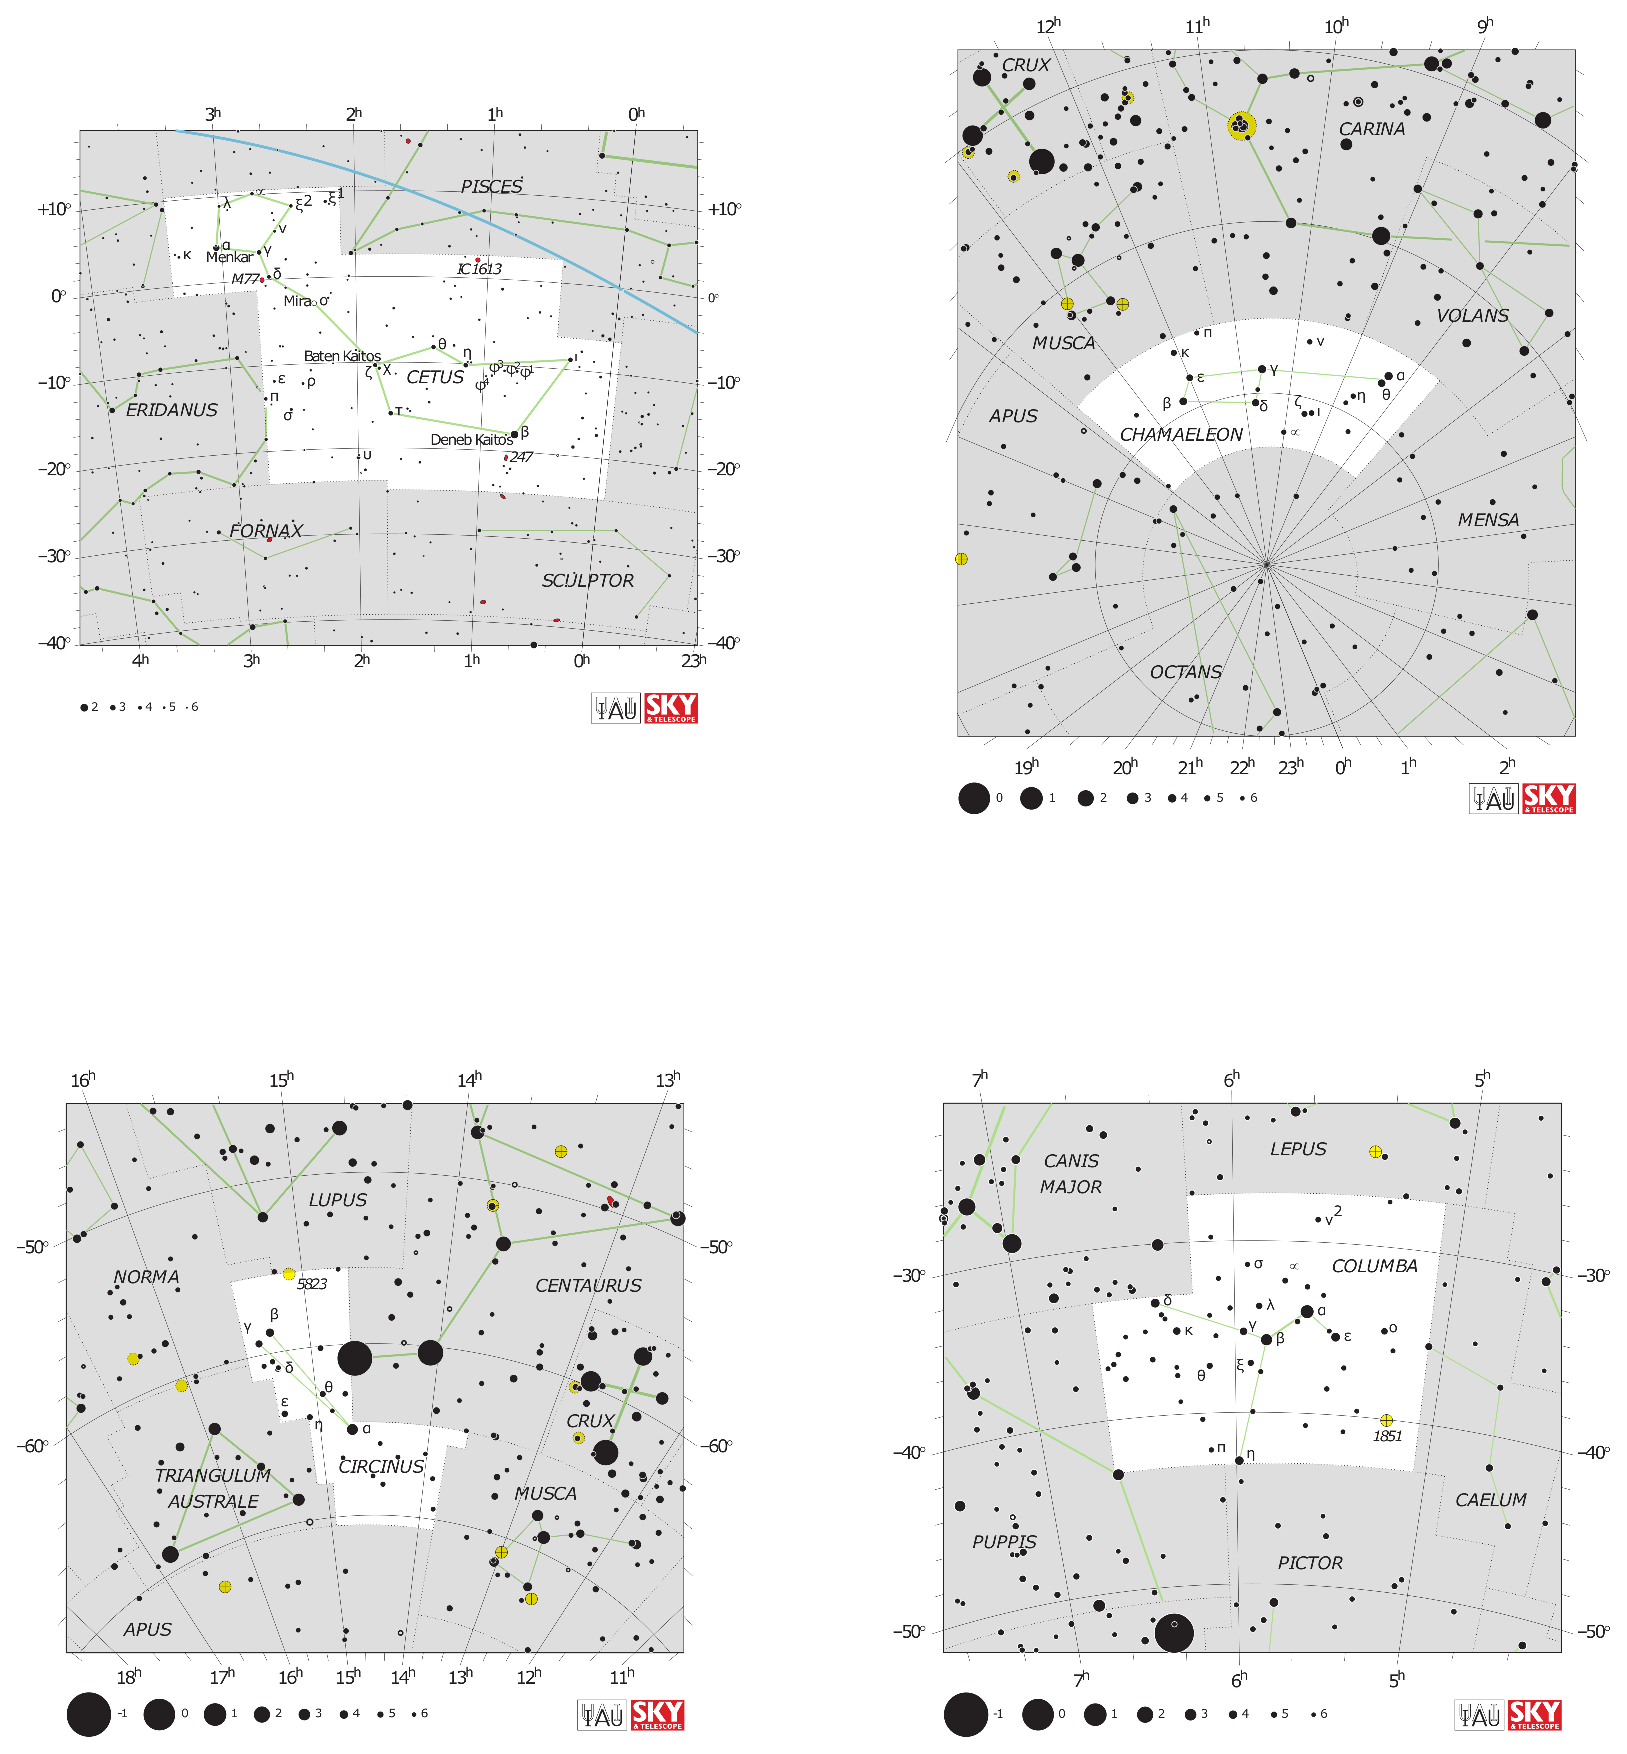
\includegraphics[width=\linewidth]{C6.eps}
\end{figure}
\clearpage
\begin{figure}
    \centering
    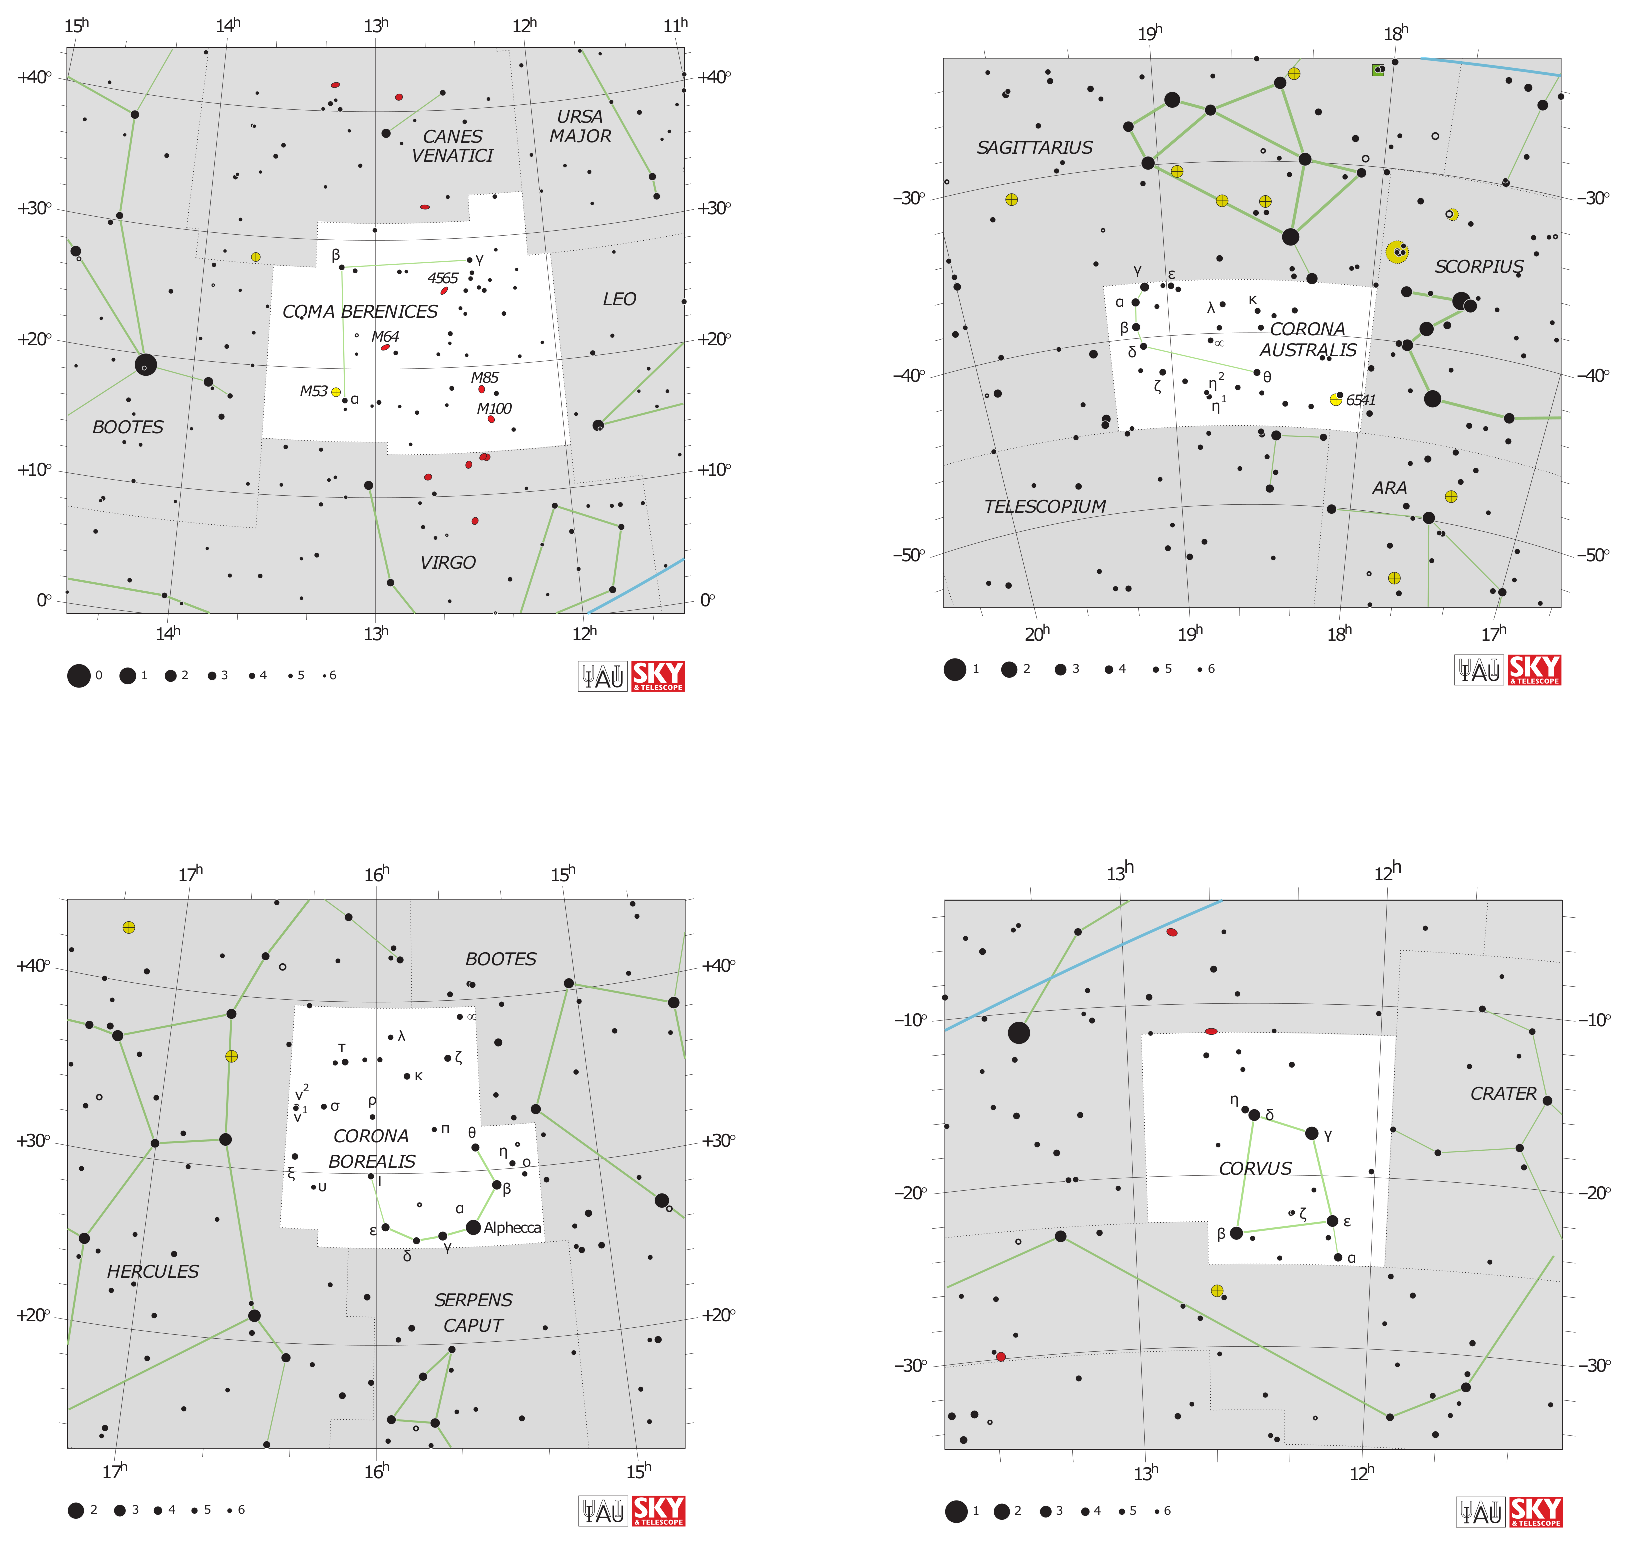
\includegraphics[width=\linewidth]{C7.eps}
\end{figure}
\clearpage
\begin{figure}
    \centering
    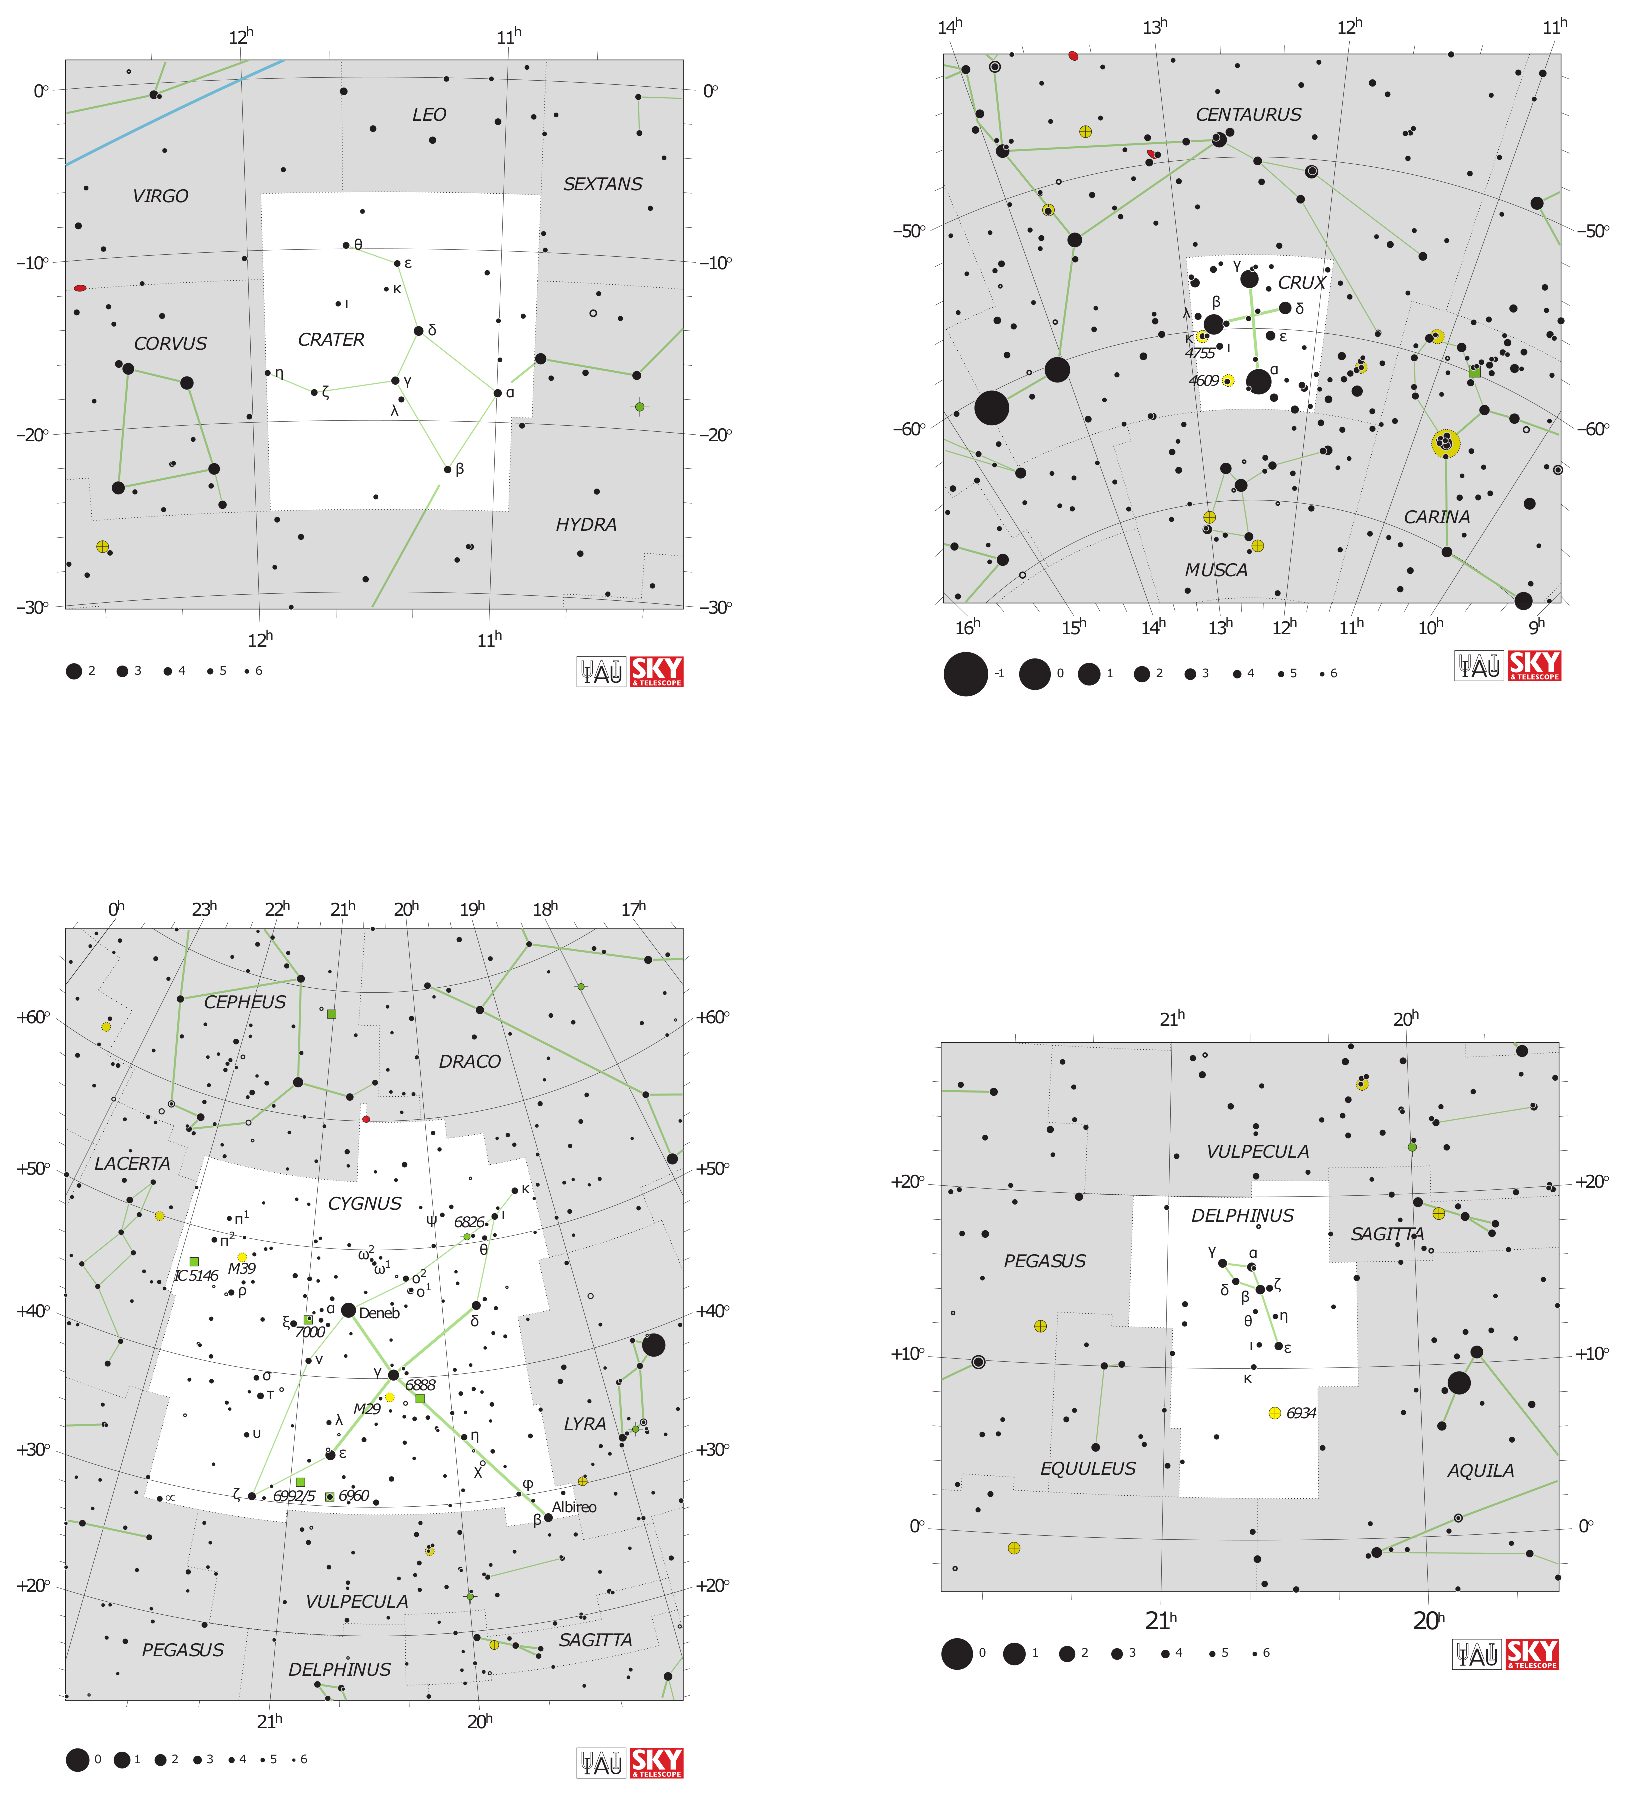
\includegraphics[width=\linewidth]{C8.eps}
\end{figure}
\clearpage
\begin{figure}
    \centering
    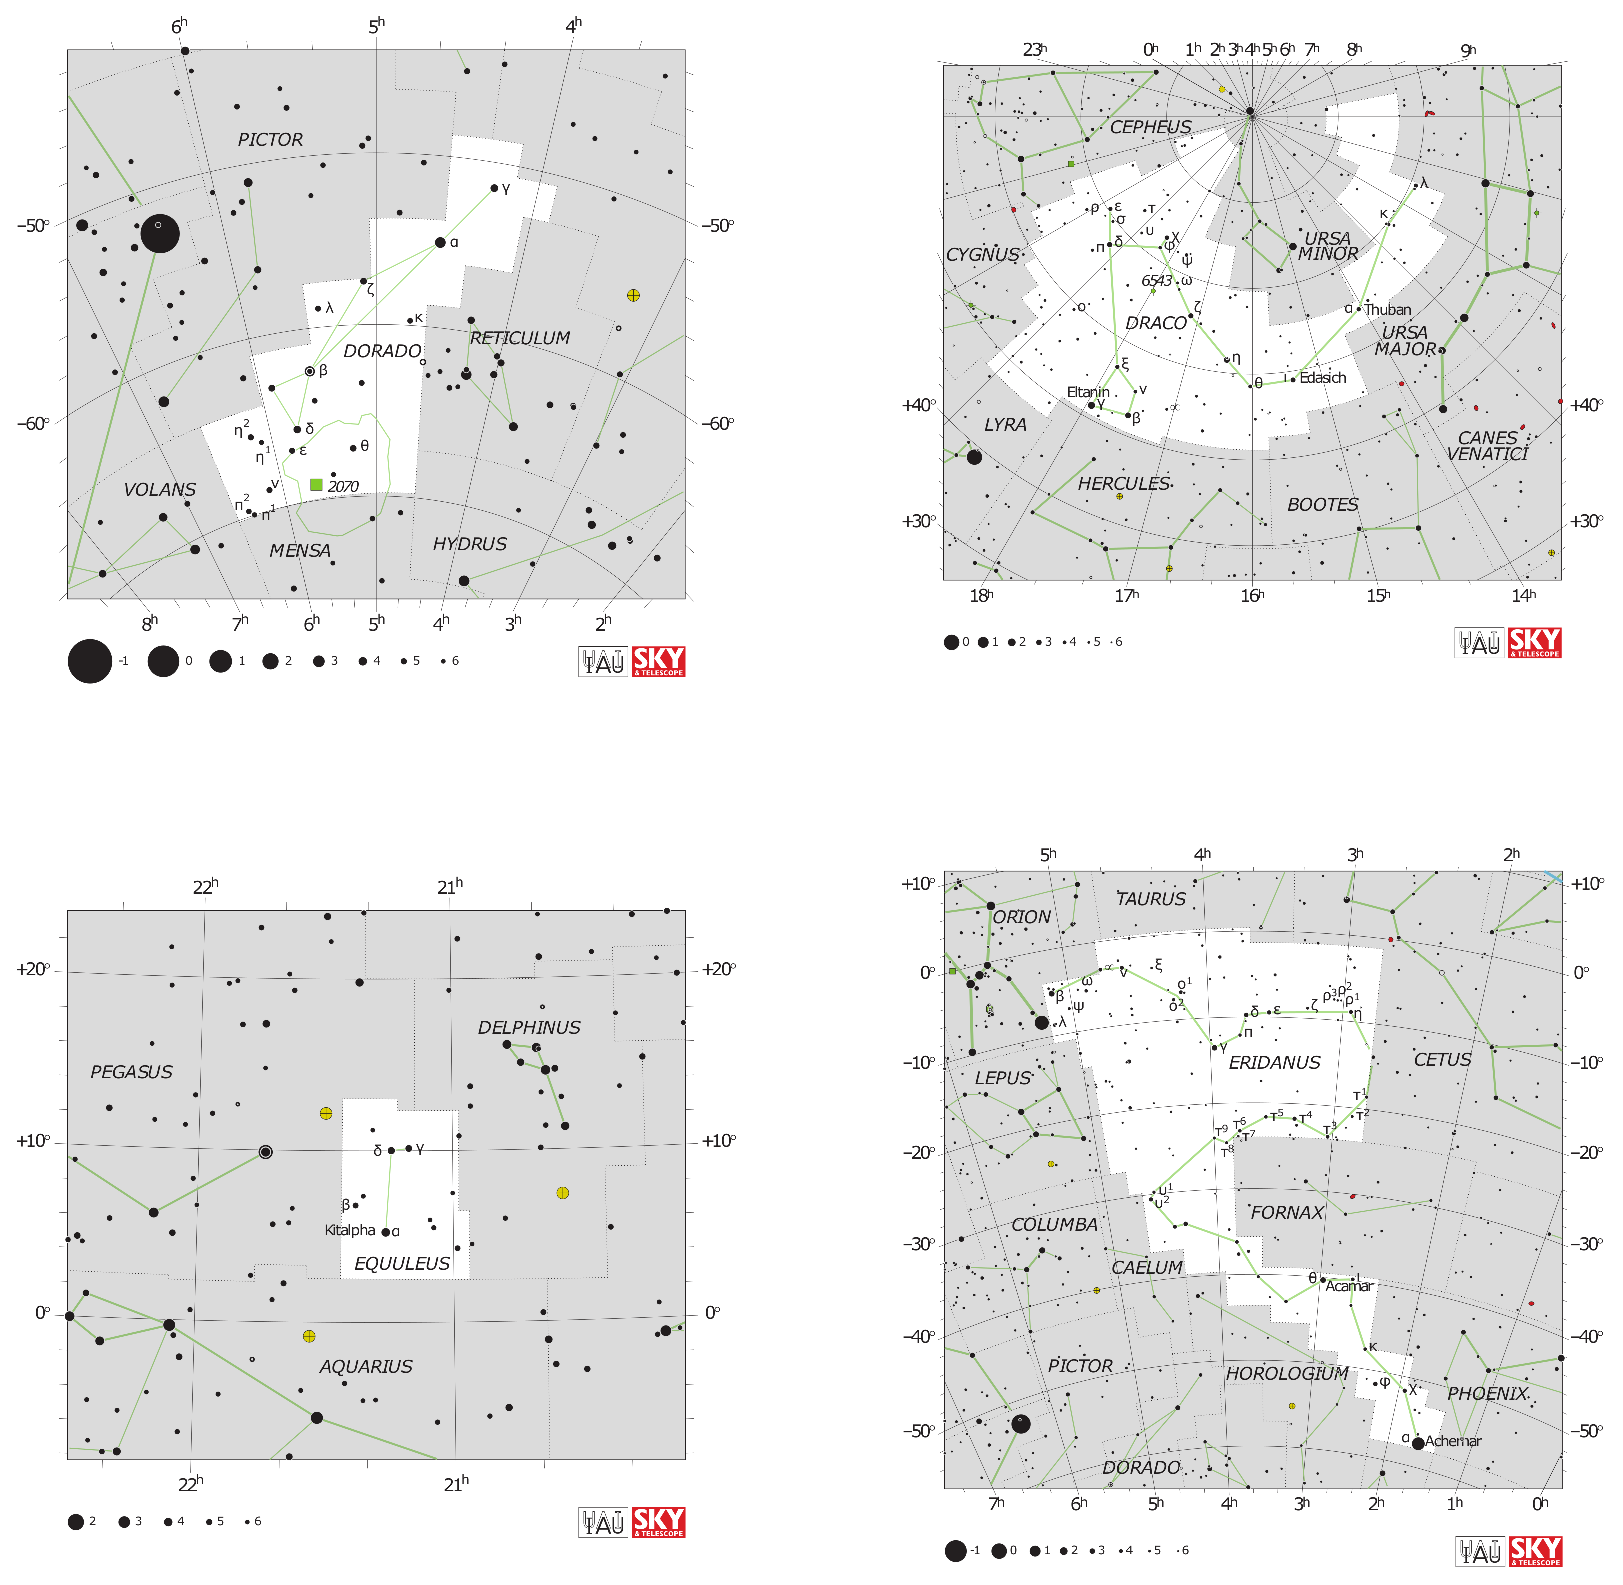
\includegraphics[width=\linewidth]{C9.eps}
\end{figure}
\clearpage
\begin{figure}
    \centering
    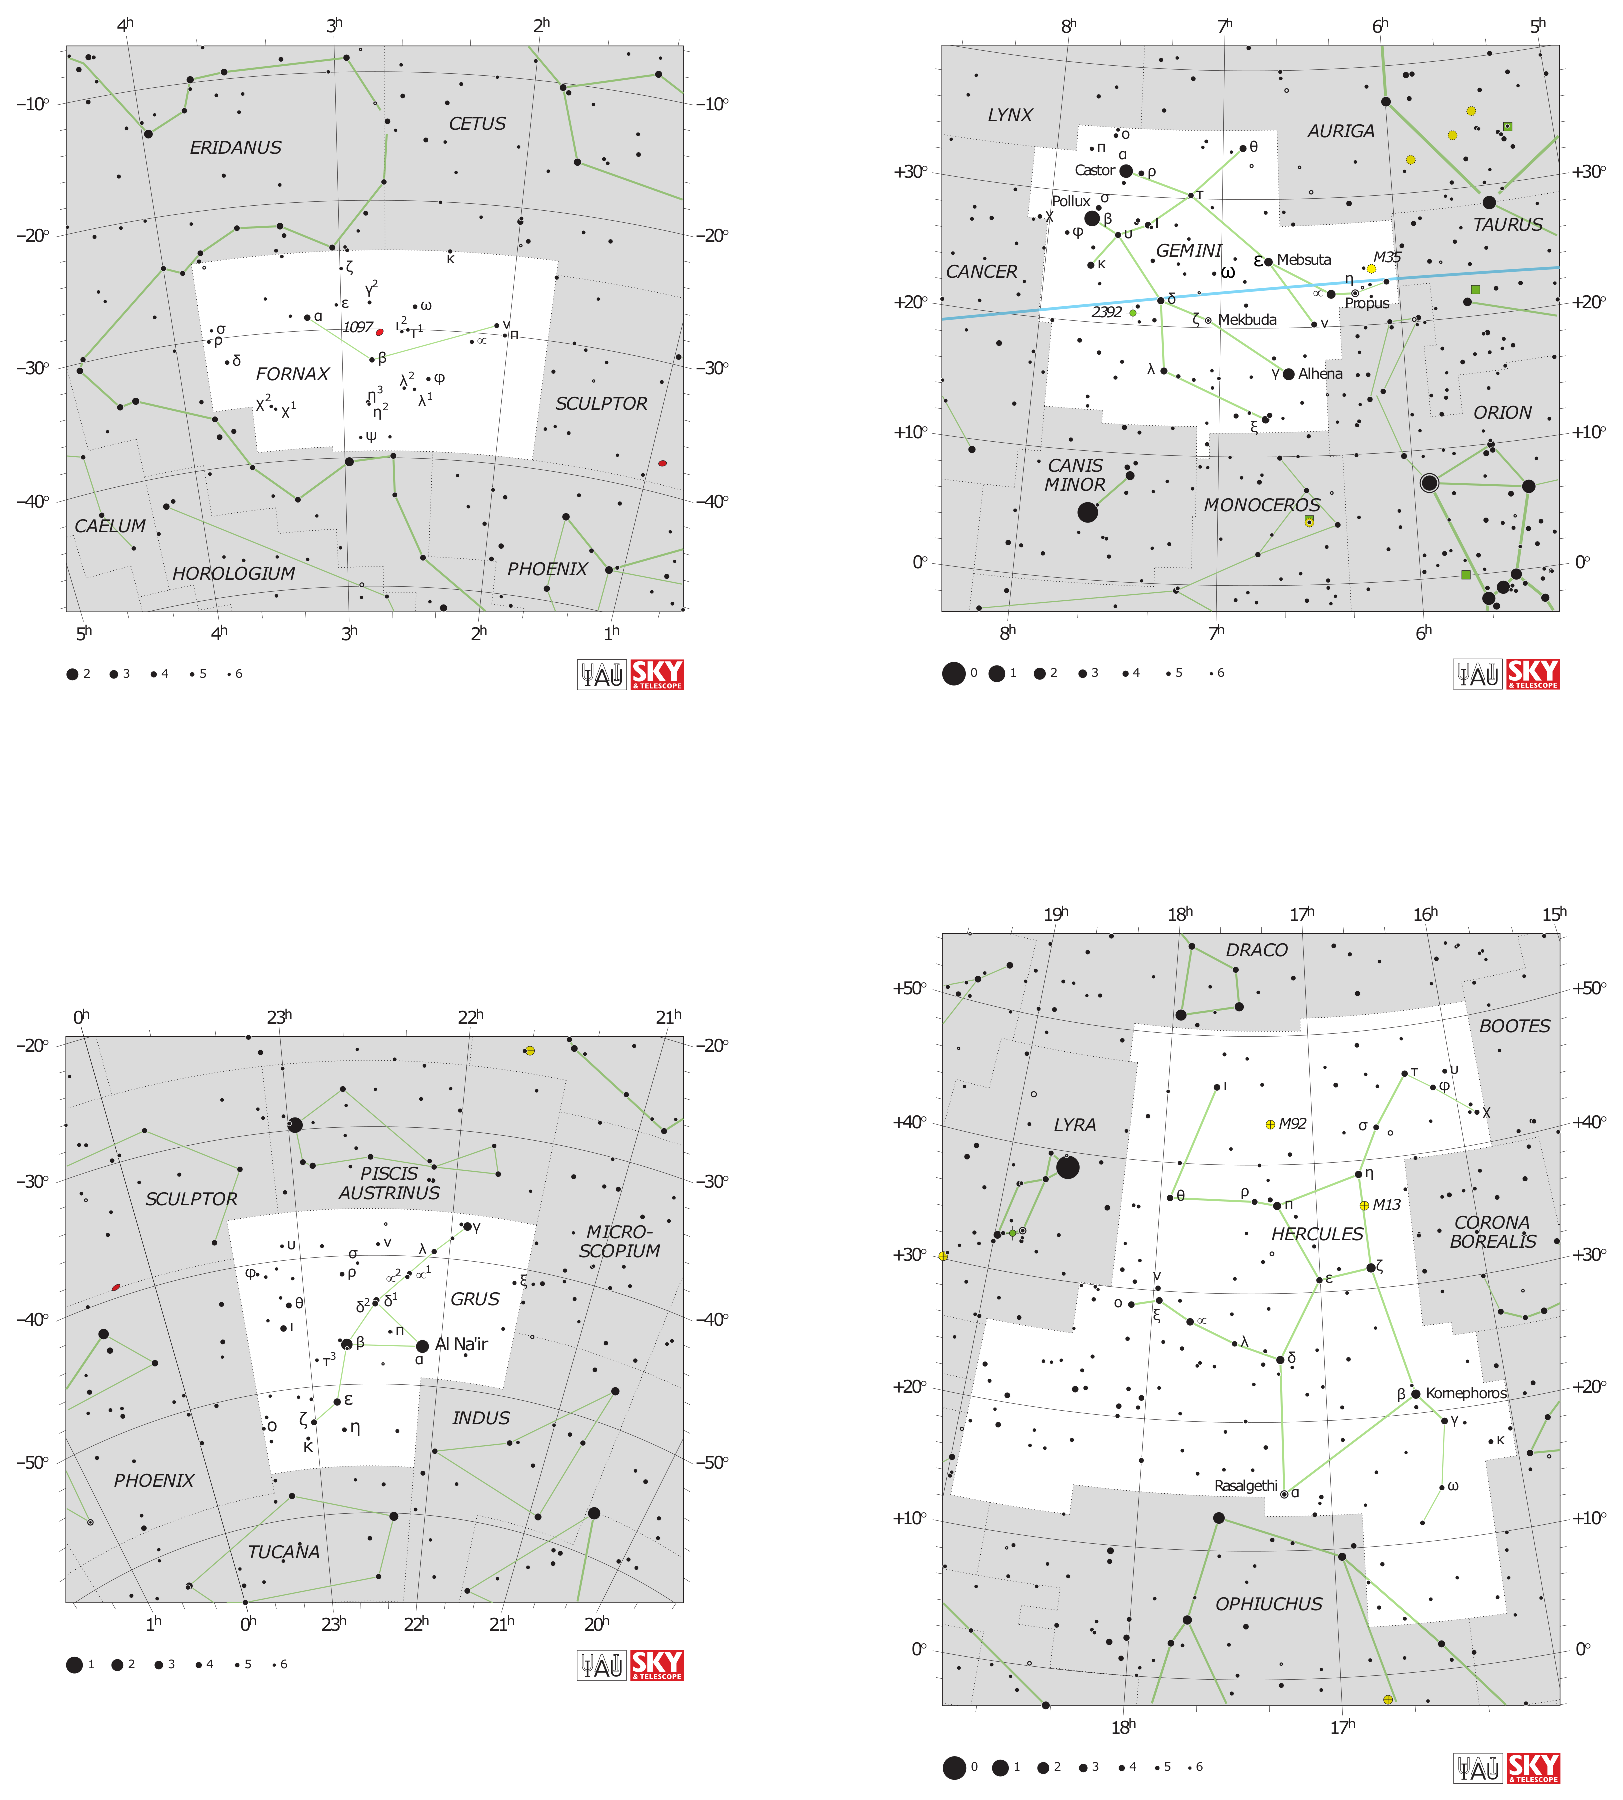
\includegraphics[width=\linewidth]{C10.eps}
\end{figure}
\clearpage
\begin{figure}
	\centering
	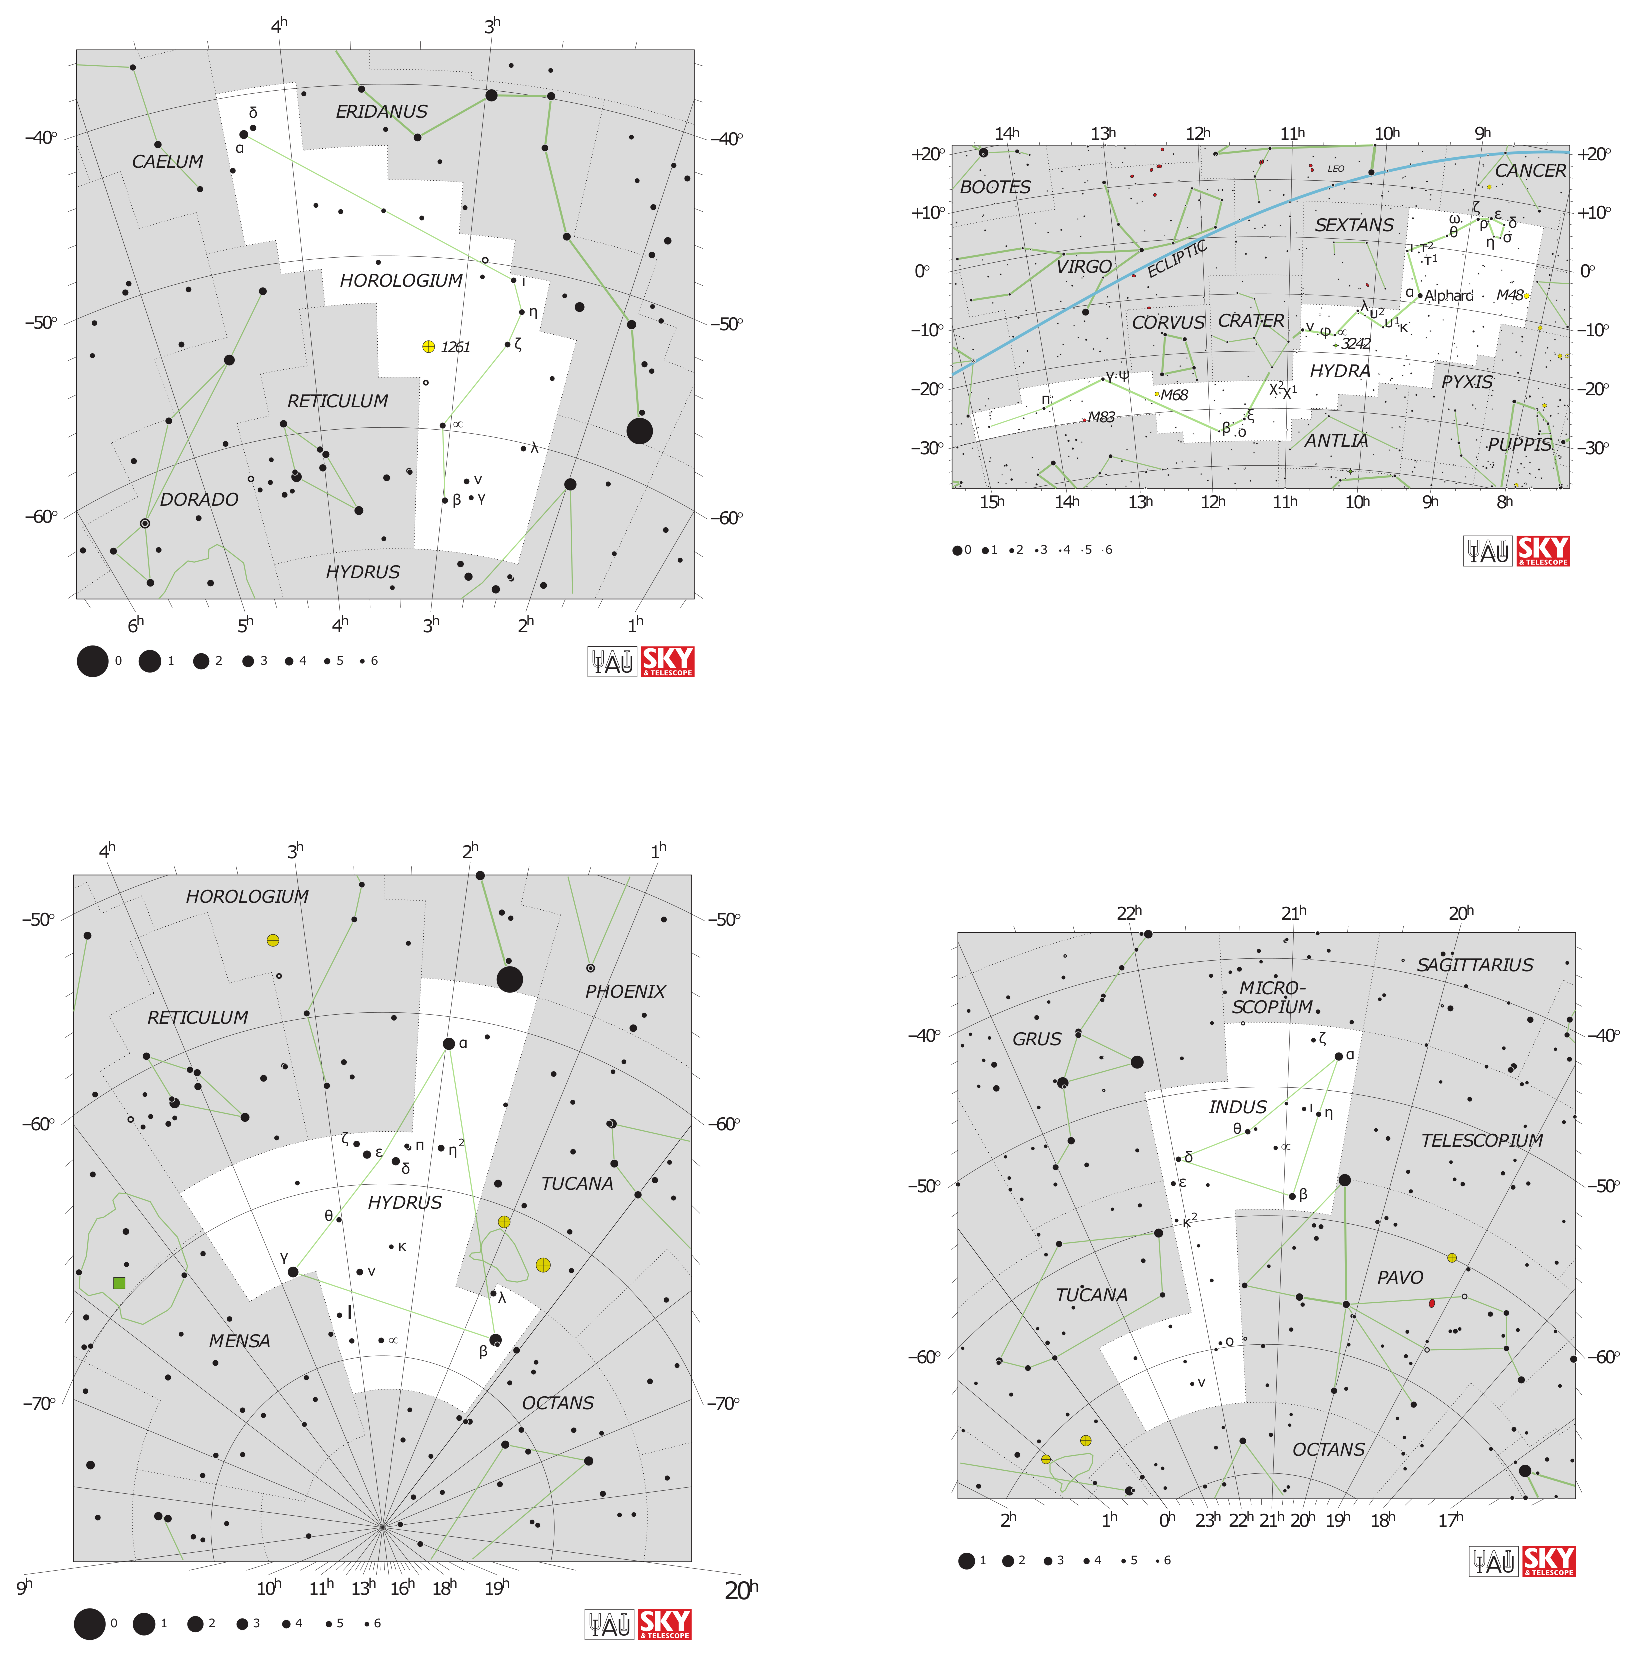
\includegraphics[width=\linewidth]{C11.eps}
\end{figure}
\clearpage
\begin{figure}
	\centering
	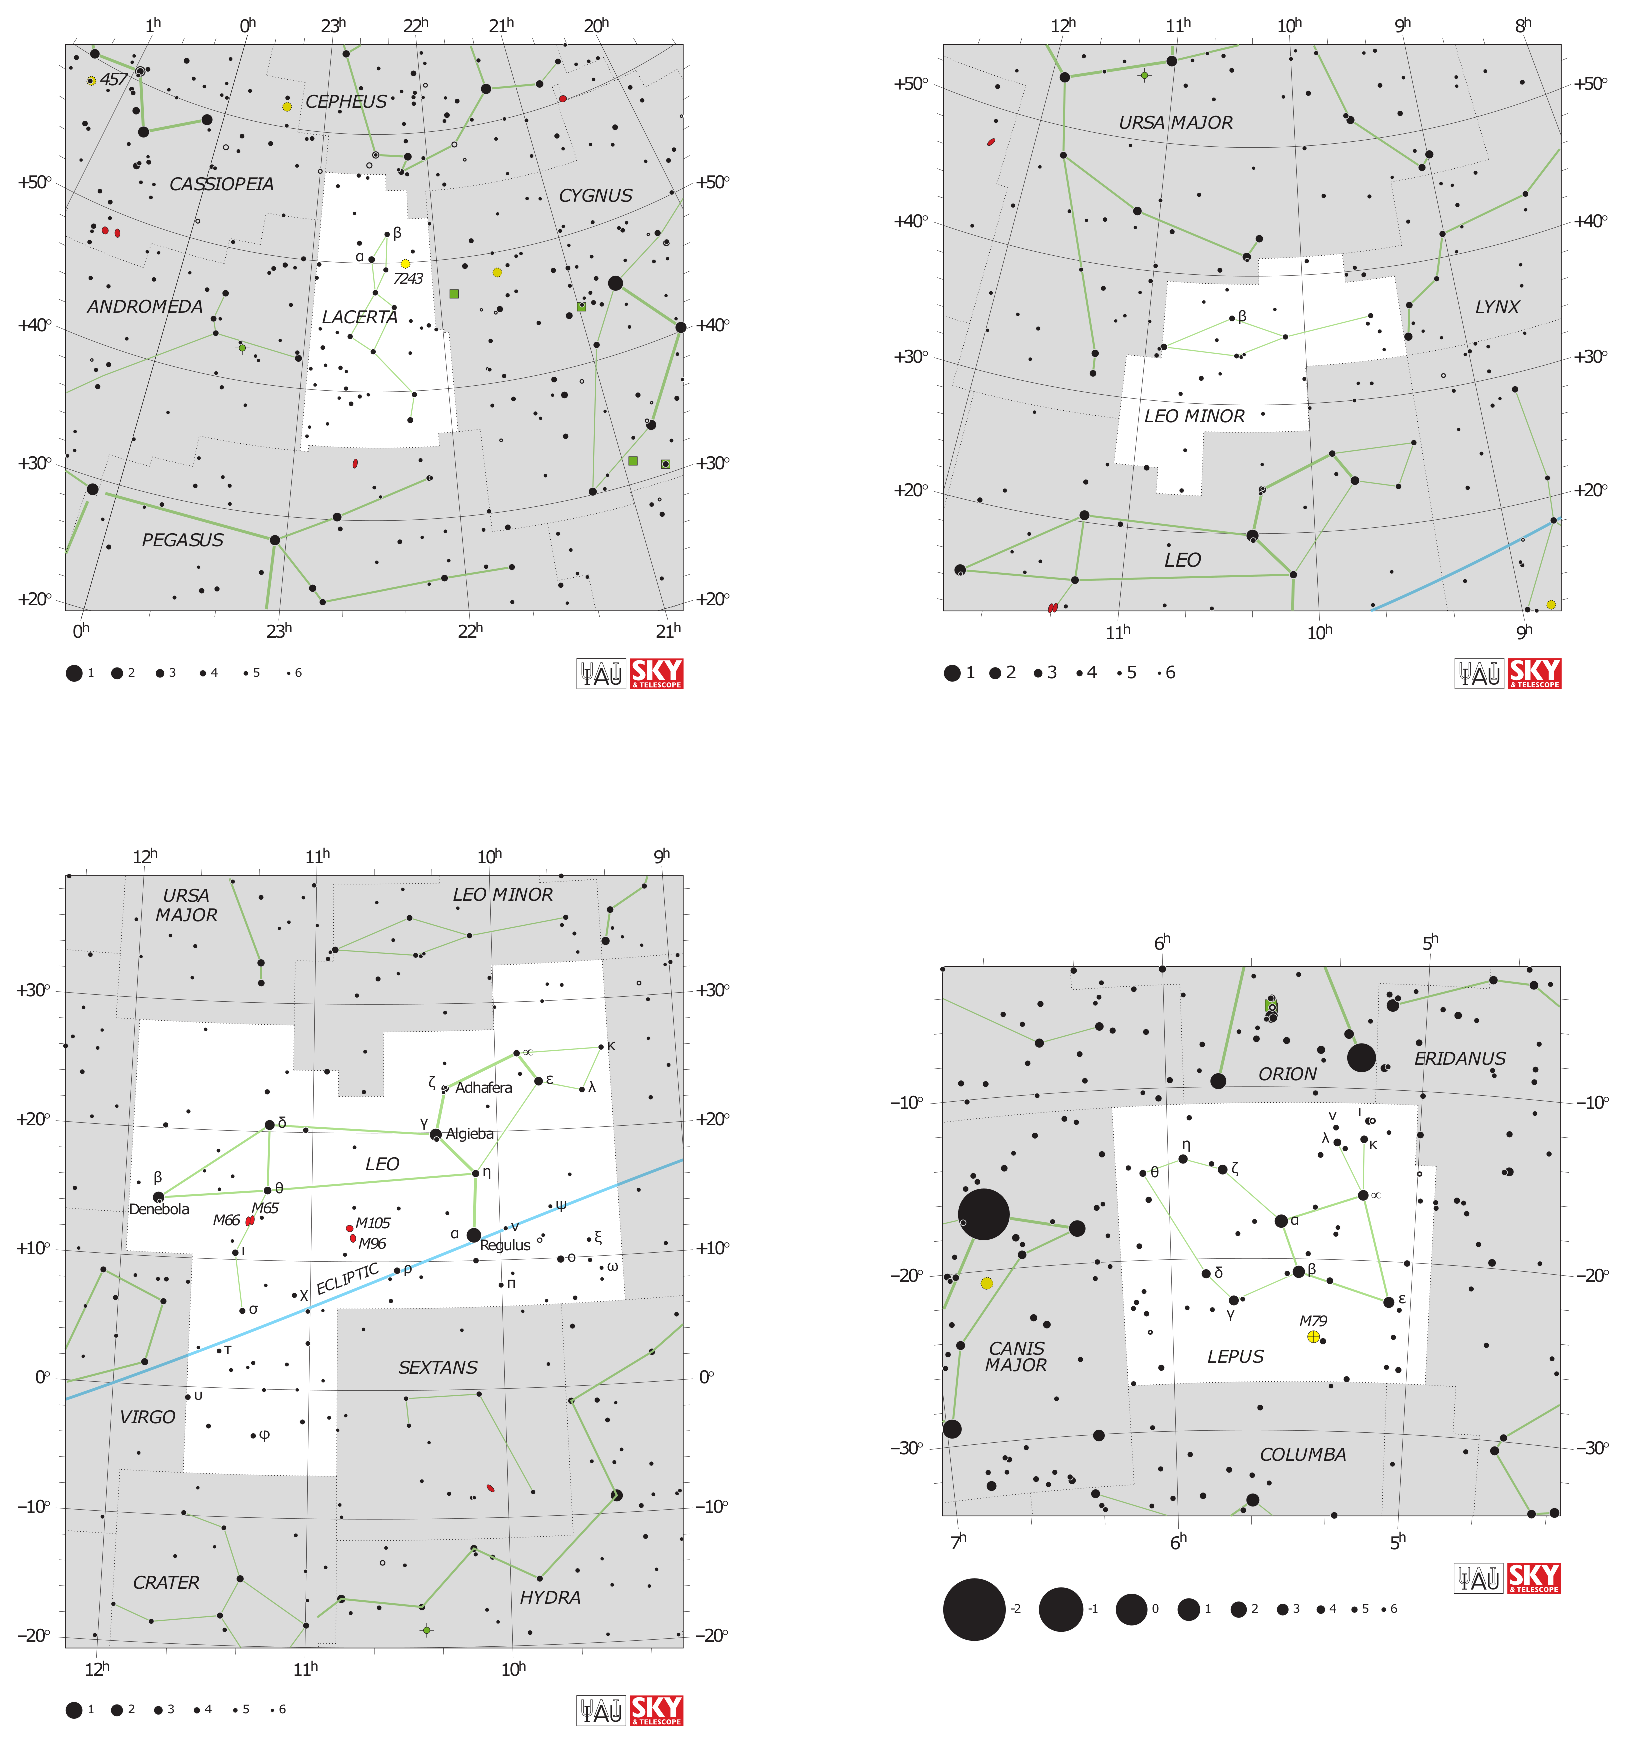
\includegraphics[width=\linewidth]{C12.eps}
\end{figure}
\clearpage
\begin{figure}
	\centering
	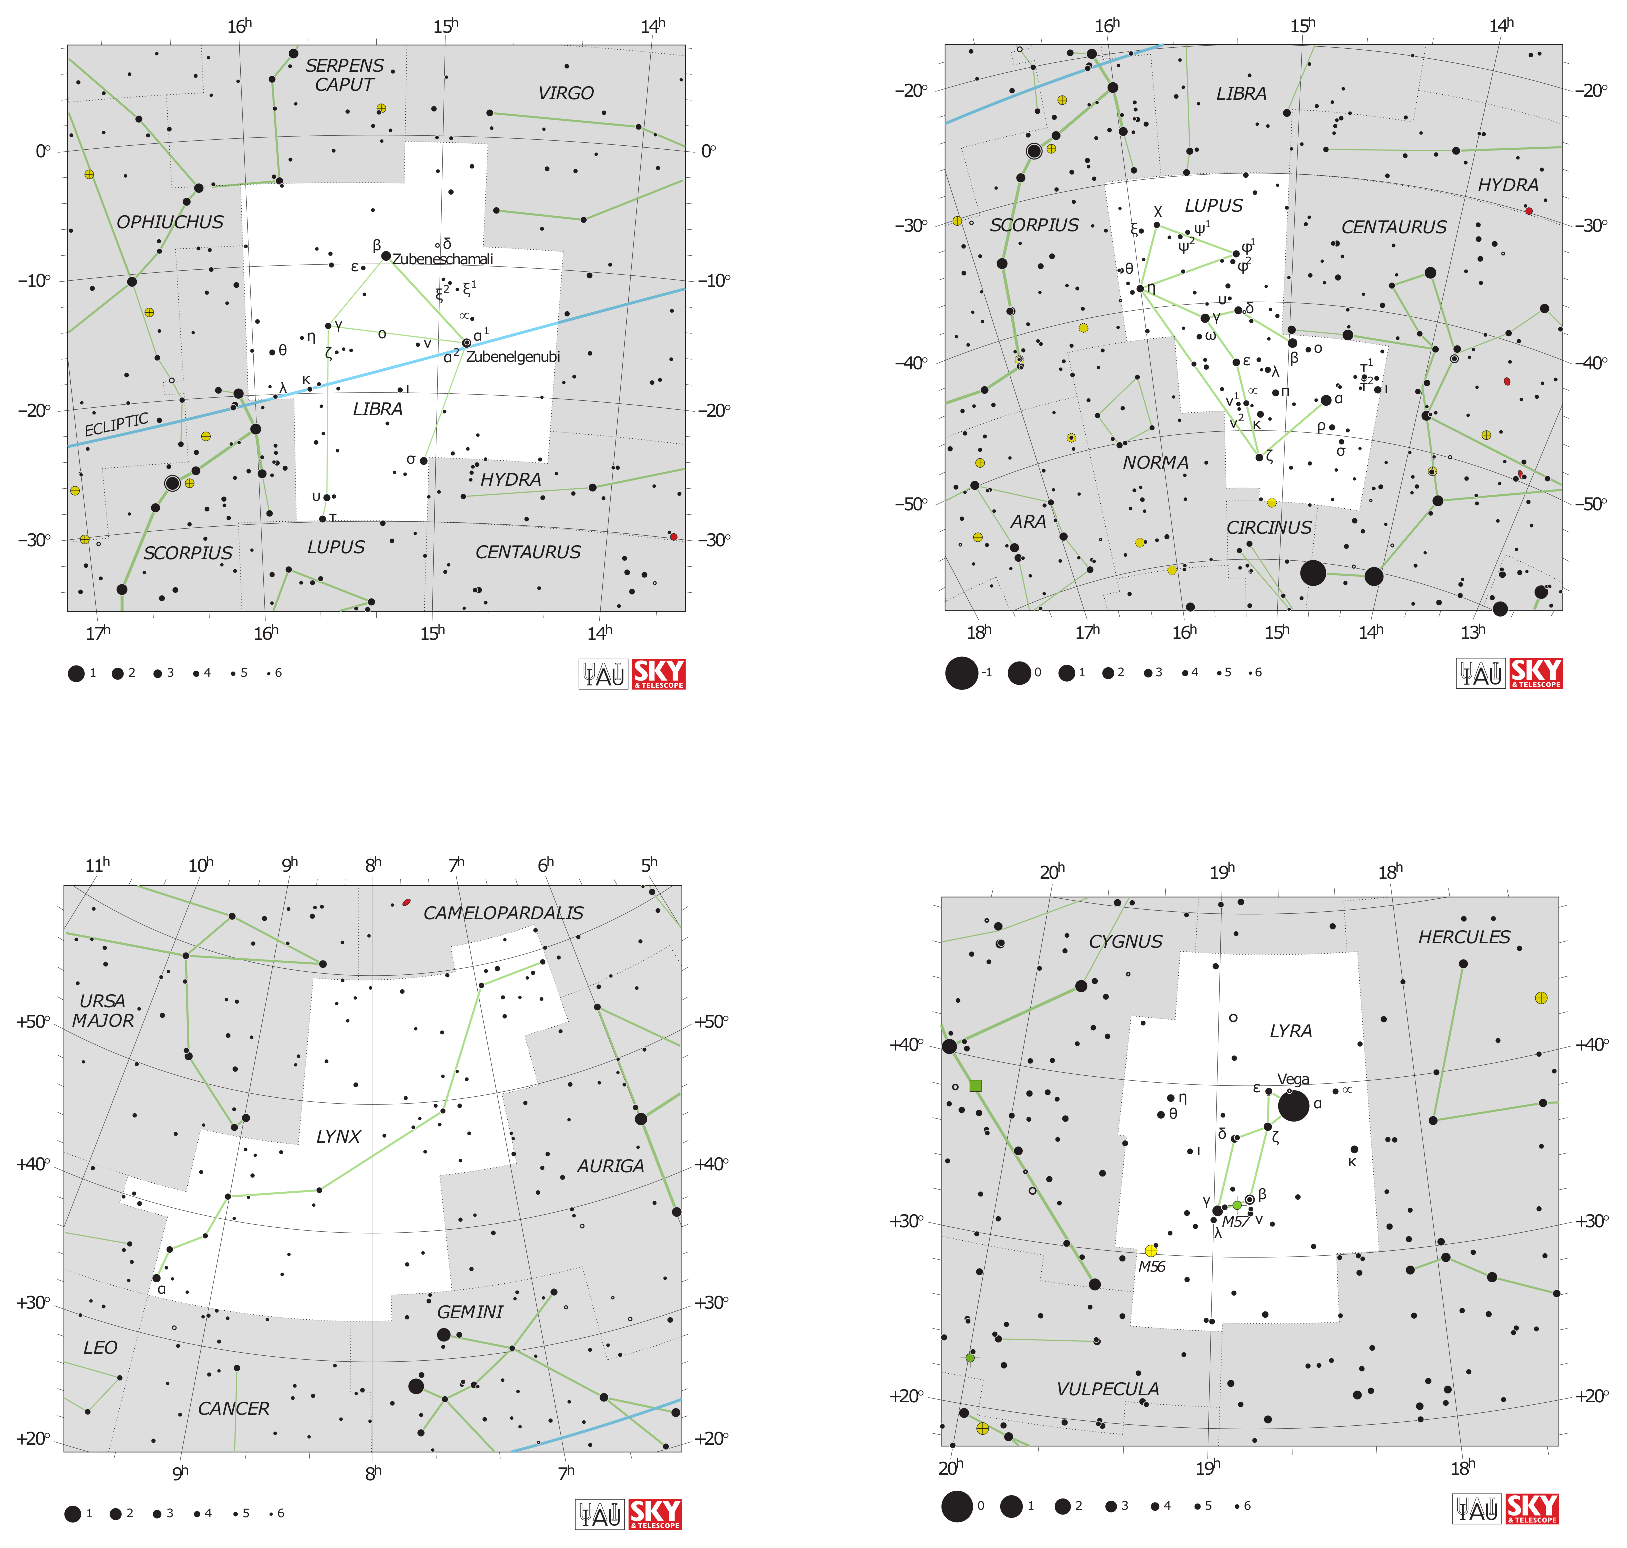
\includegraphics[width=\linewidth]{C13.eps}
\end{figure}
\clearpage
\begin{figure}
	\centering
	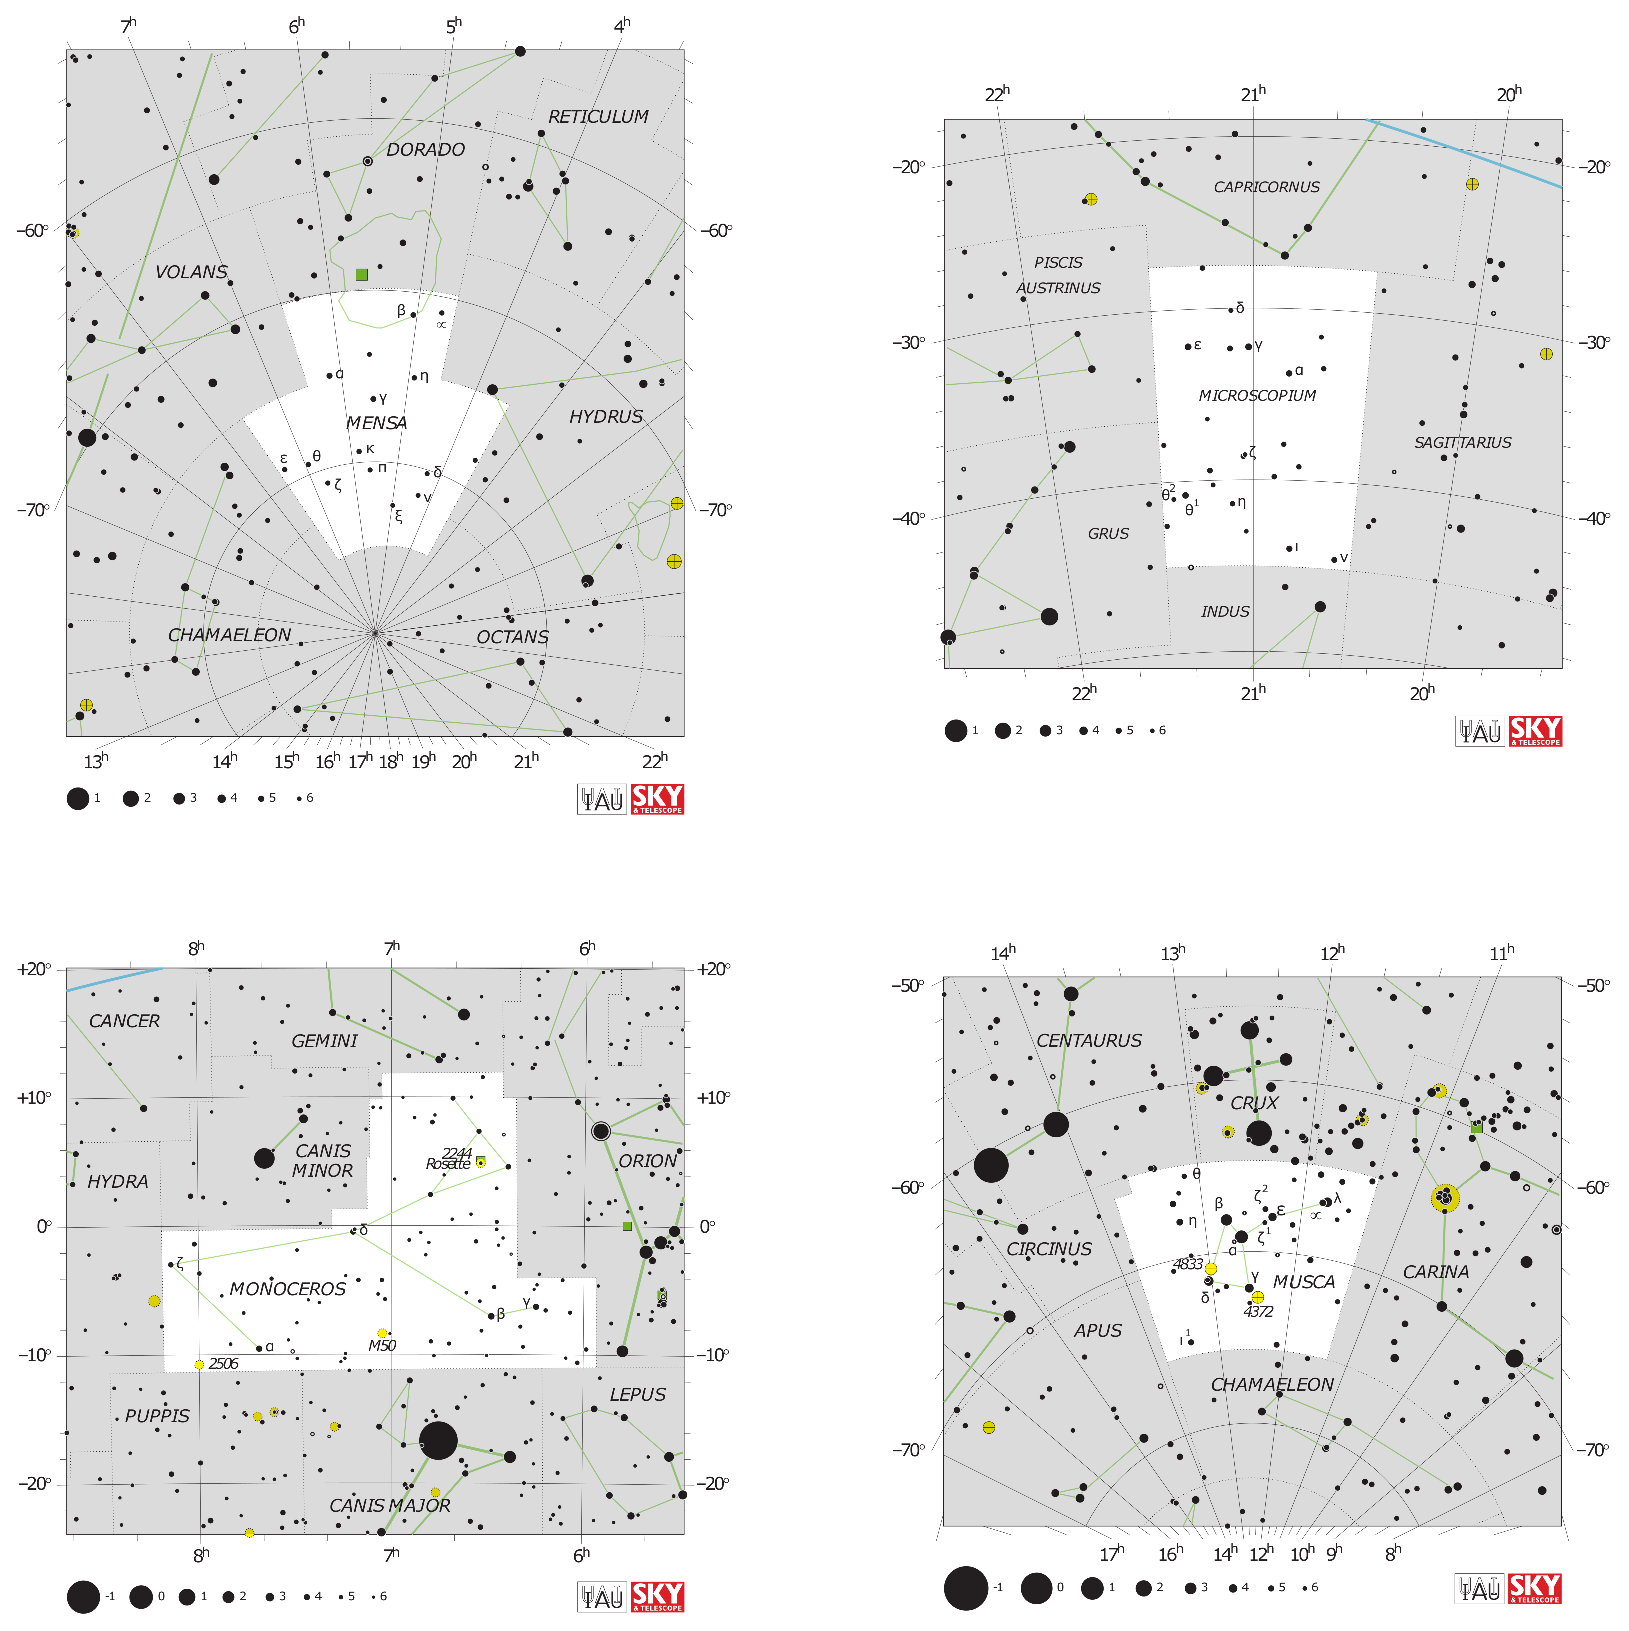
\includegraphics[width=\linewidth]{C14.eps}
\end{figure}
\clearpage
\begin{figure}
	\centering
	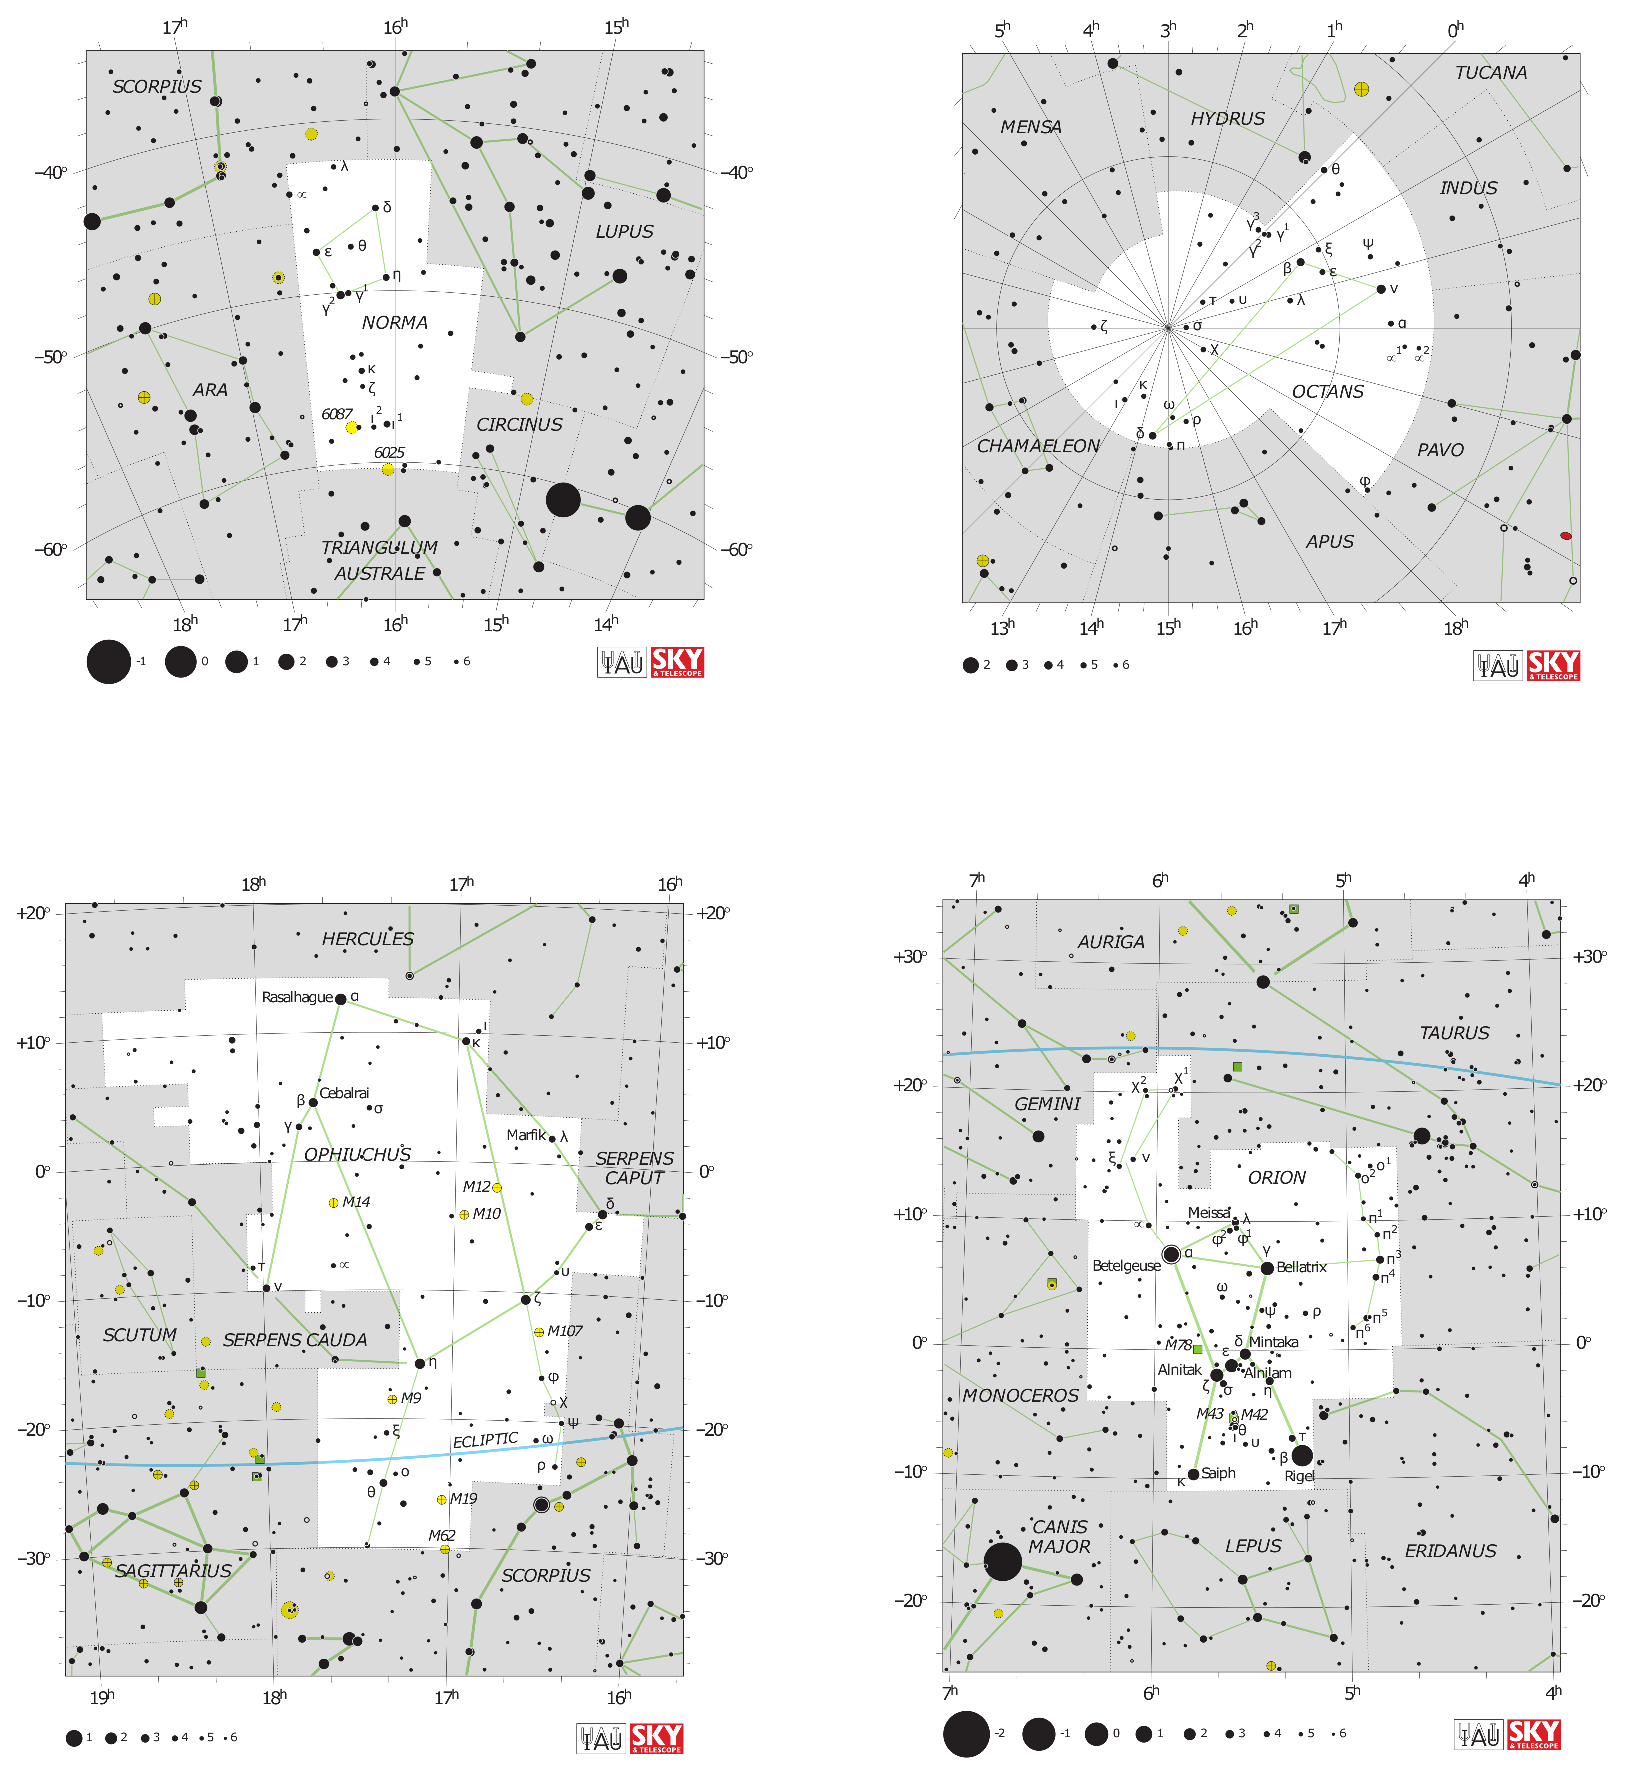
\includegraphics[width=\linewidth]{C15.eps}
\end{figure}
\begin{figure}
	\centering
	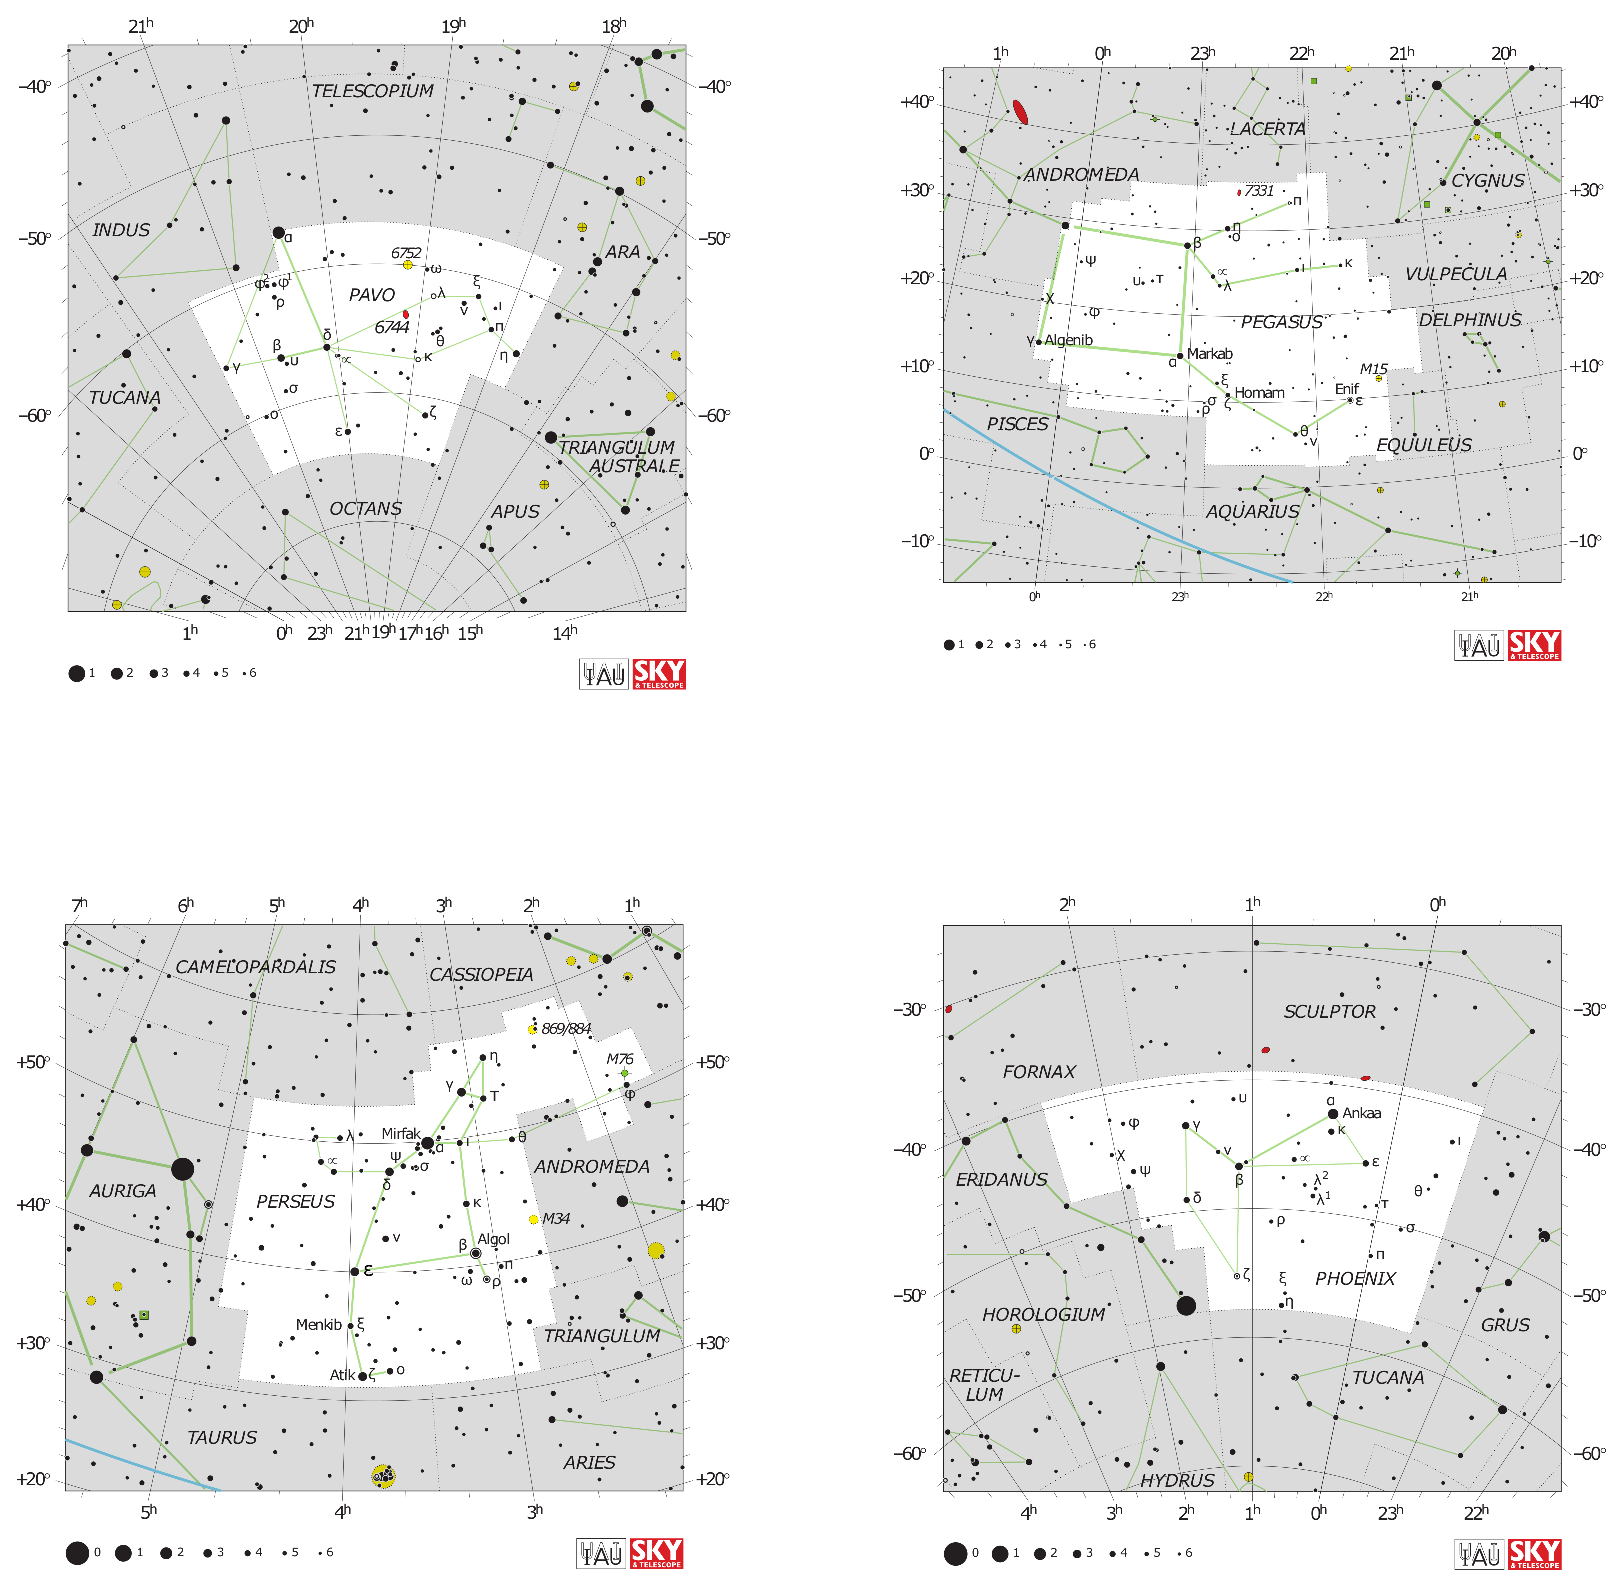
\includegraphics[width=\linewidth]{C16.eps}
\end{figure}
\clearpage
\begin{figure}
	\centering
	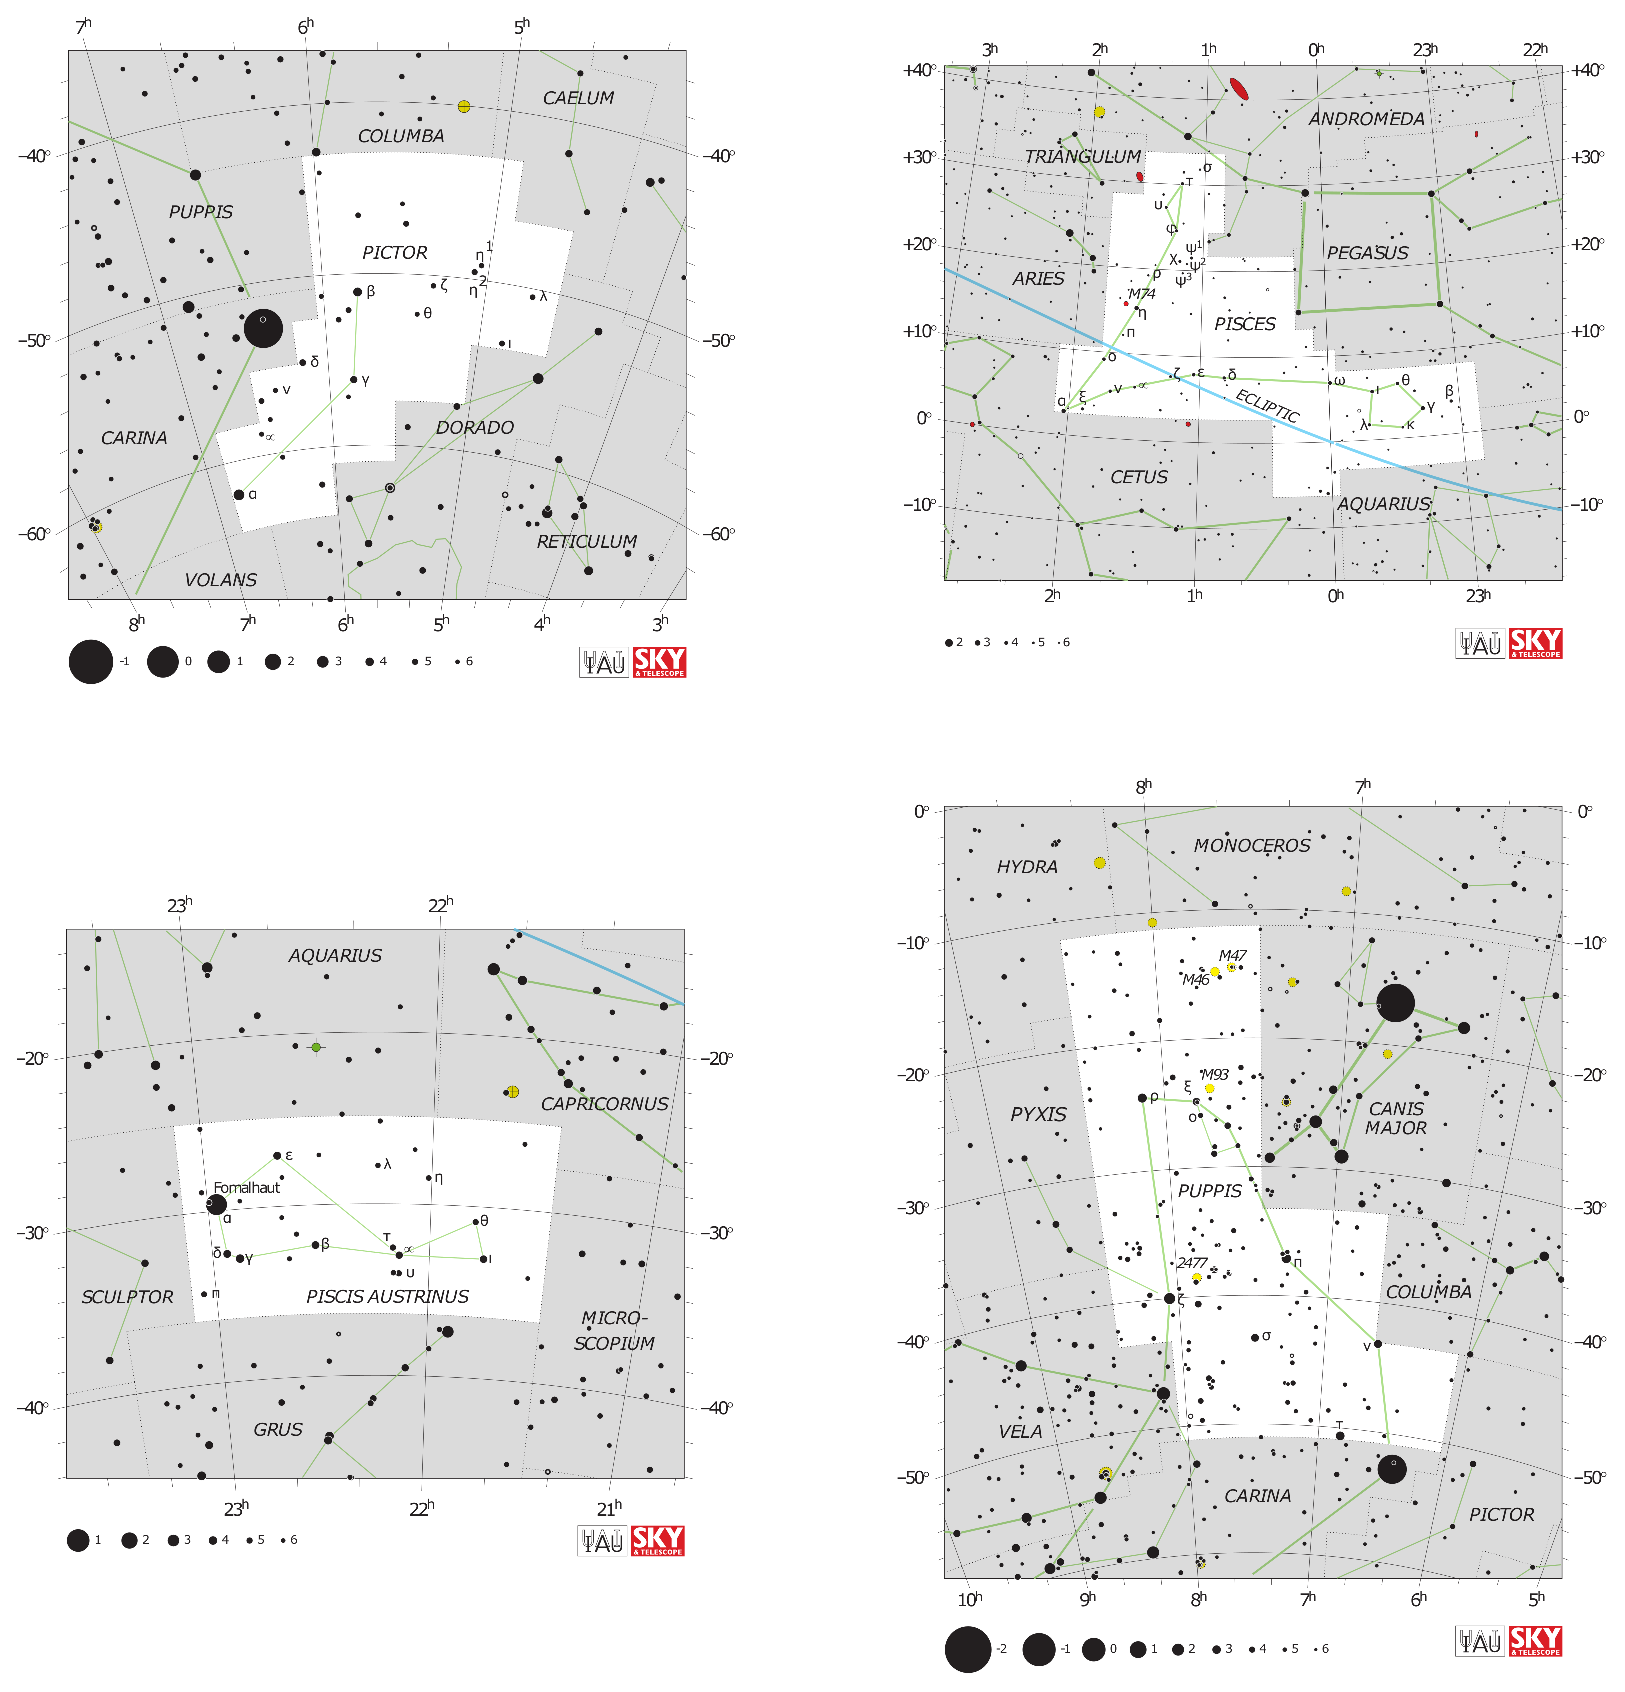
\includegraphics[width=\linewidth]{C17.eps}
\end{figure}
\clearpage
\begin{figure}
	\centering
	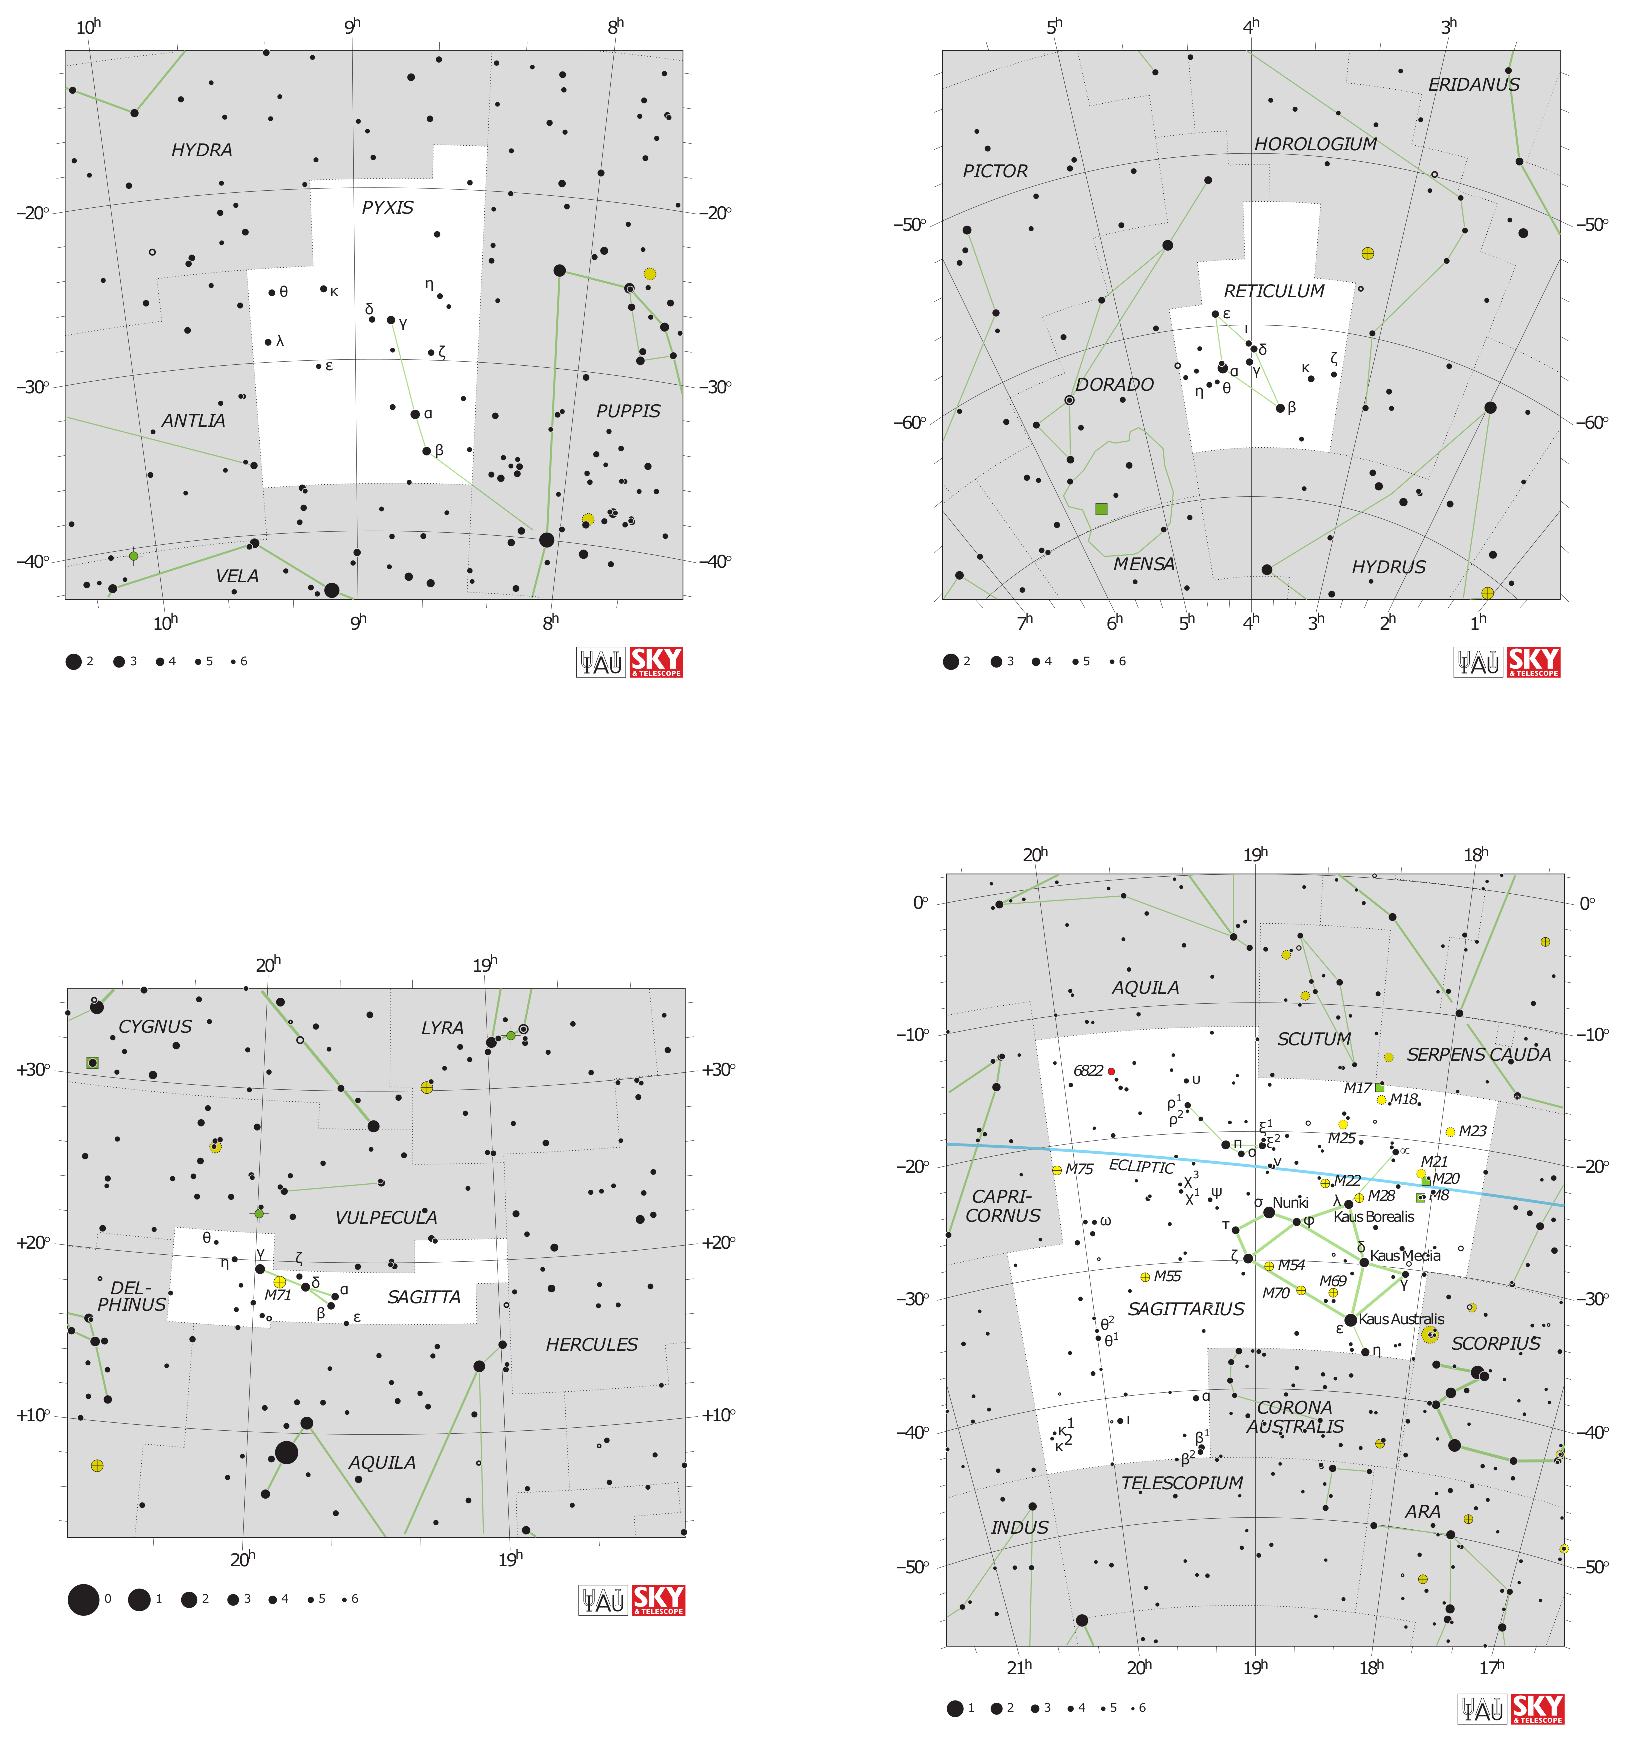
\includegraphics[width=\linewidth]{C18.eps}
\end{figure}
\clearpage
\begin{figure}
	\centering
	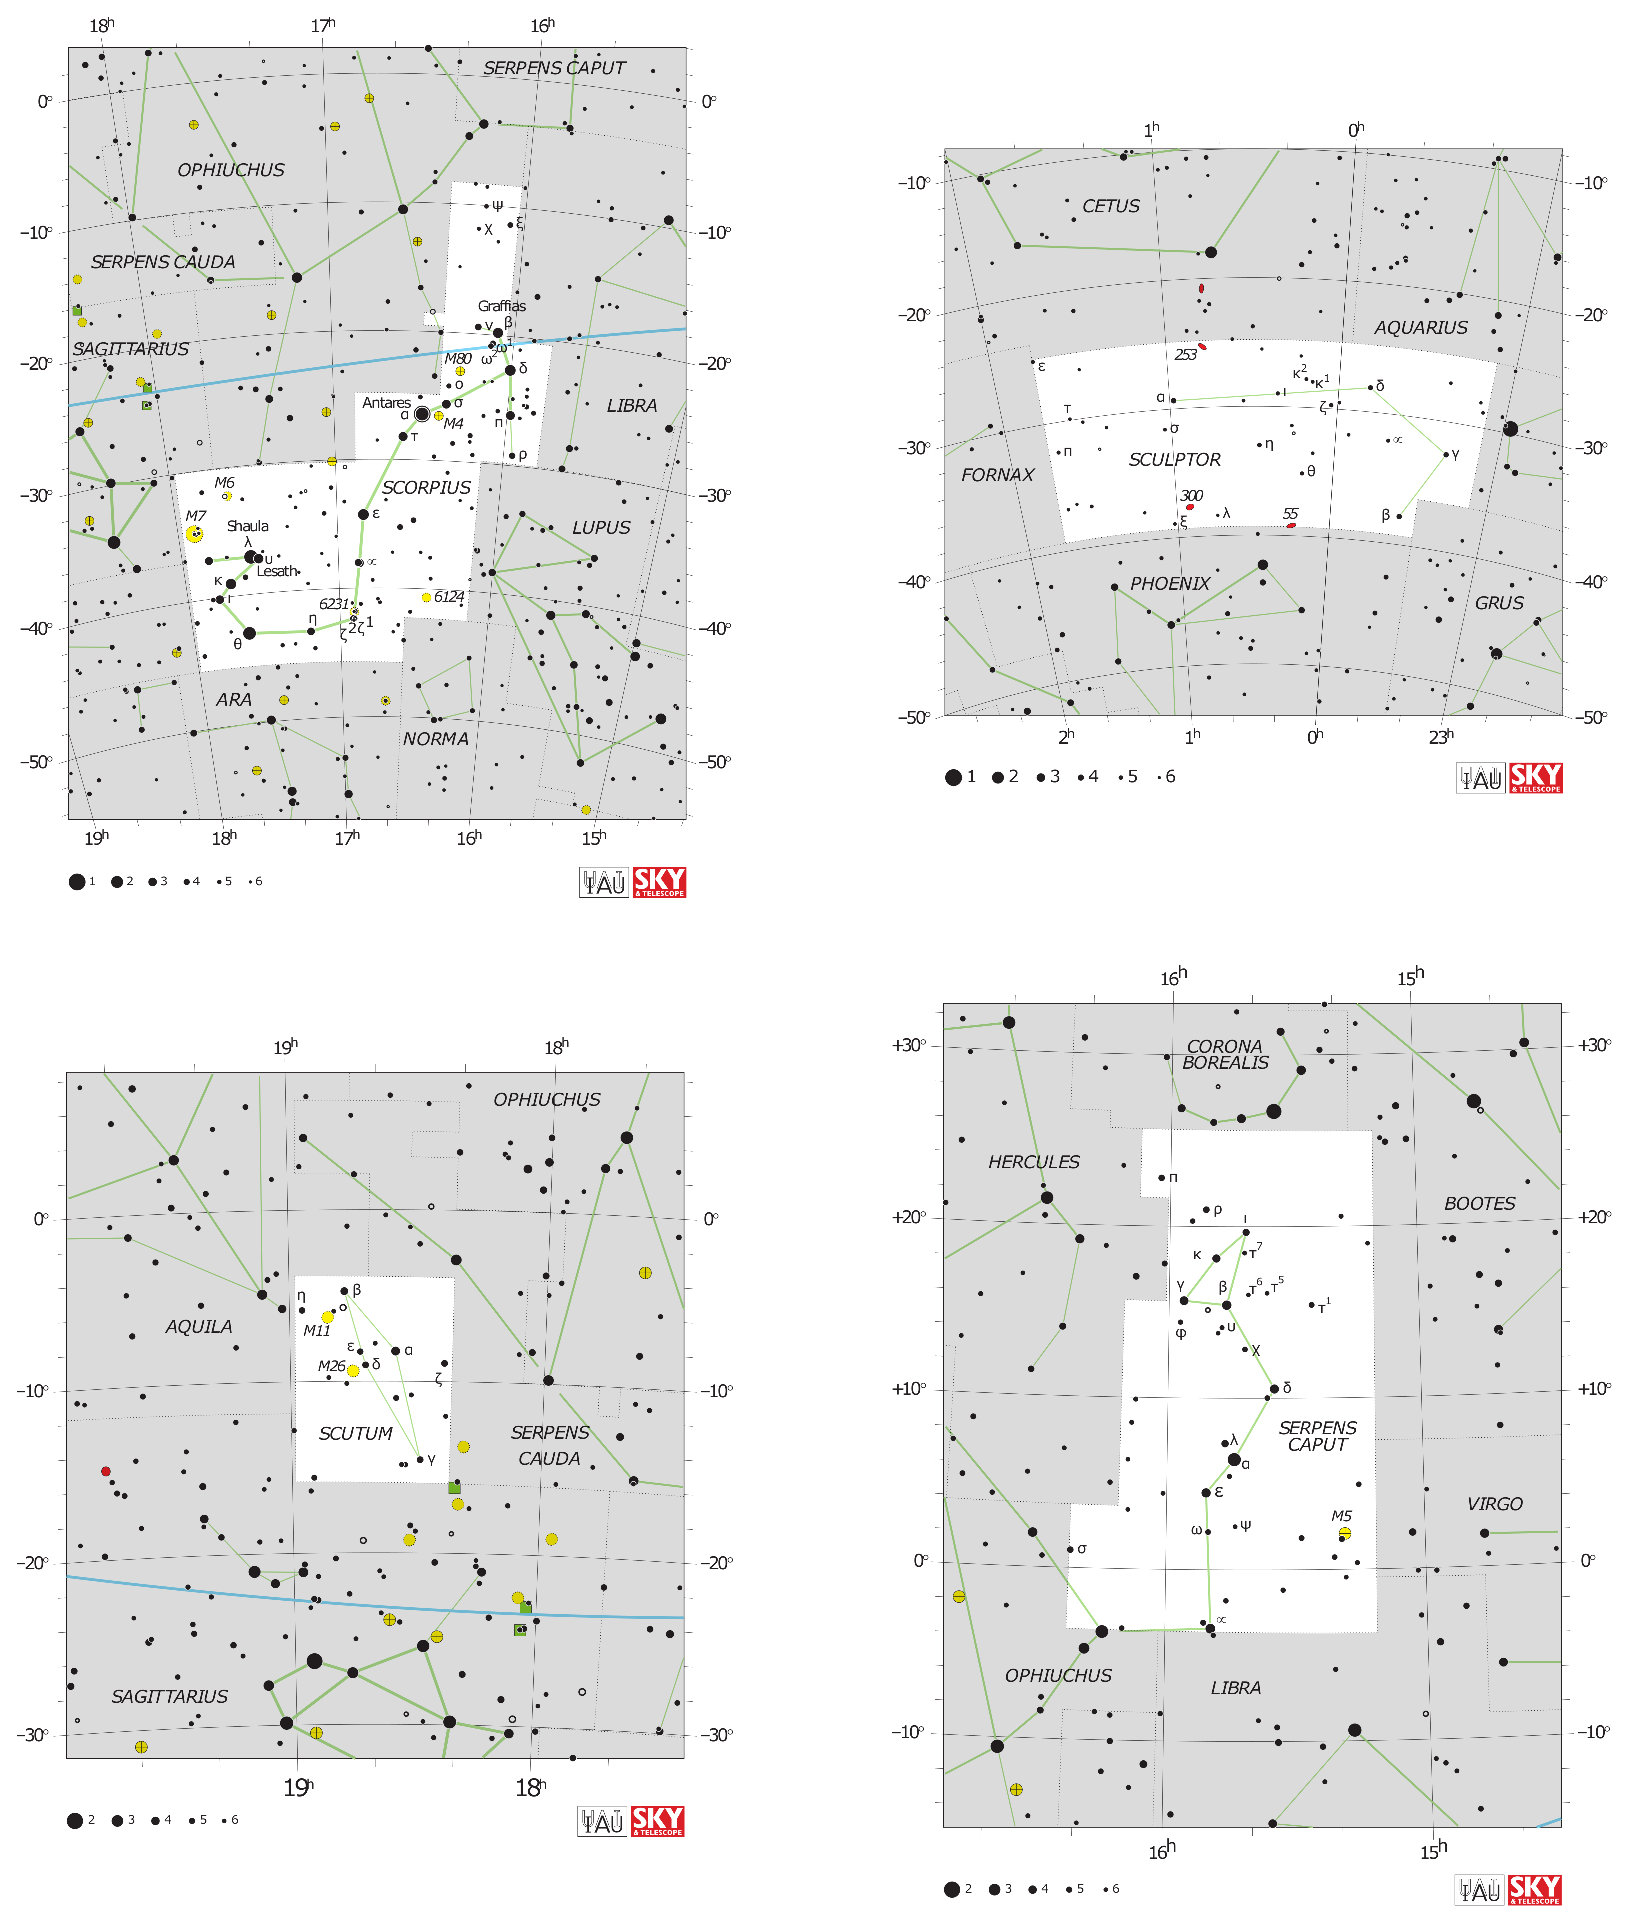
\includegraphics[width=\linewidth]{C19.eps}
\end{figure}
\clearpage
\begin{figure}
	\centering
	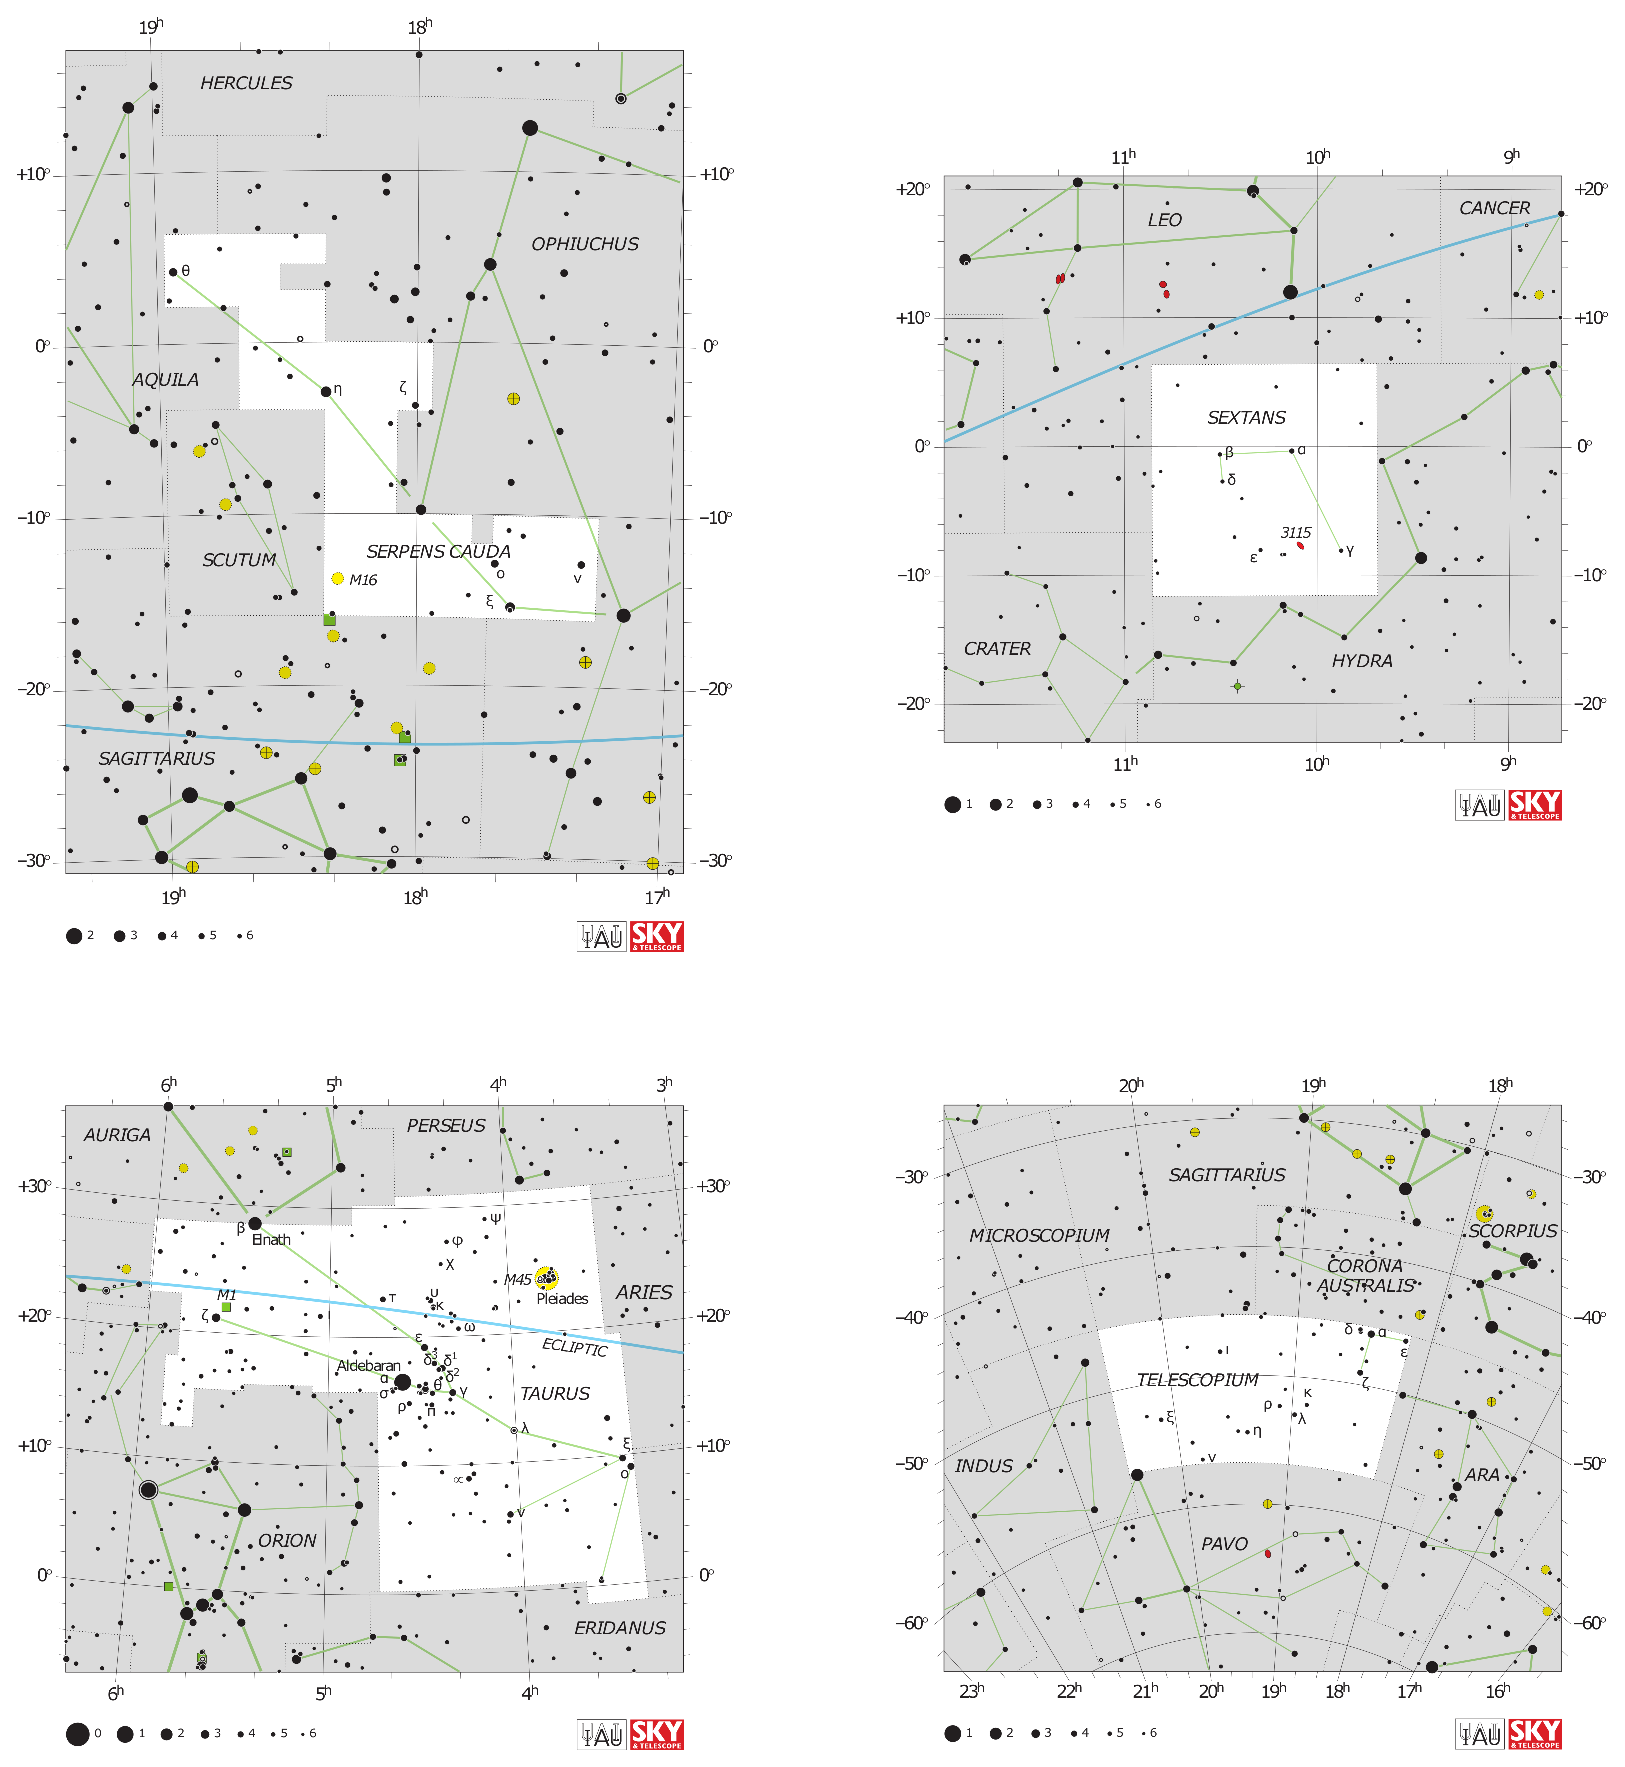
\includegraphics[width=\linewidth]{C20.eps}
\end{figure}
\clearpage
\begin{figure}
	\centering
	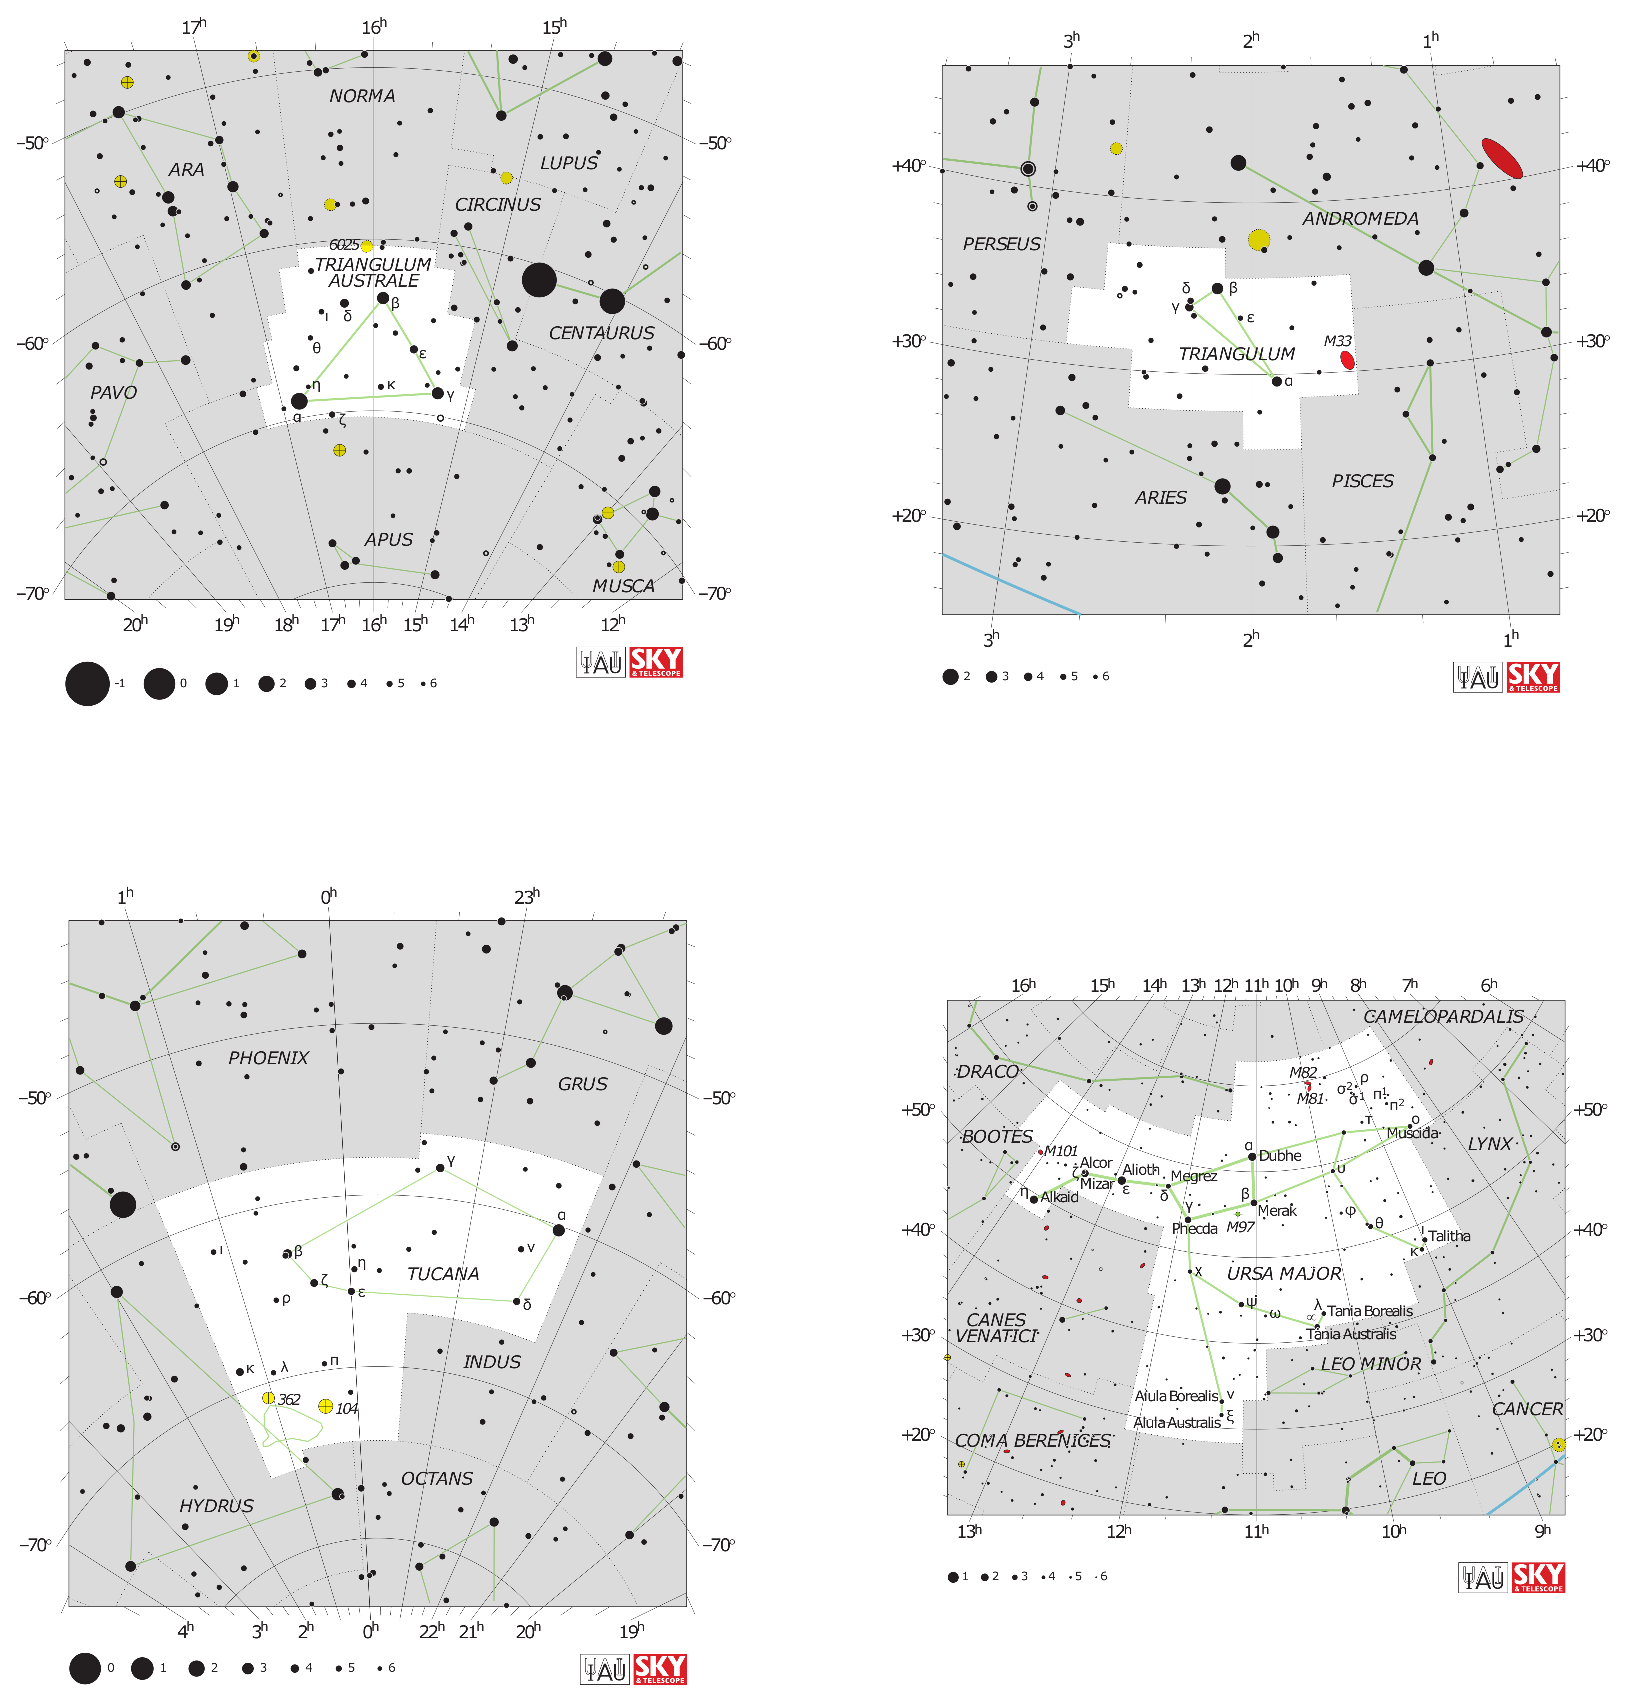
\includegraphics[width=\linewidth]{C21.eps}
\end{figure}
\clearpage
\begin{figure}
	\centering
	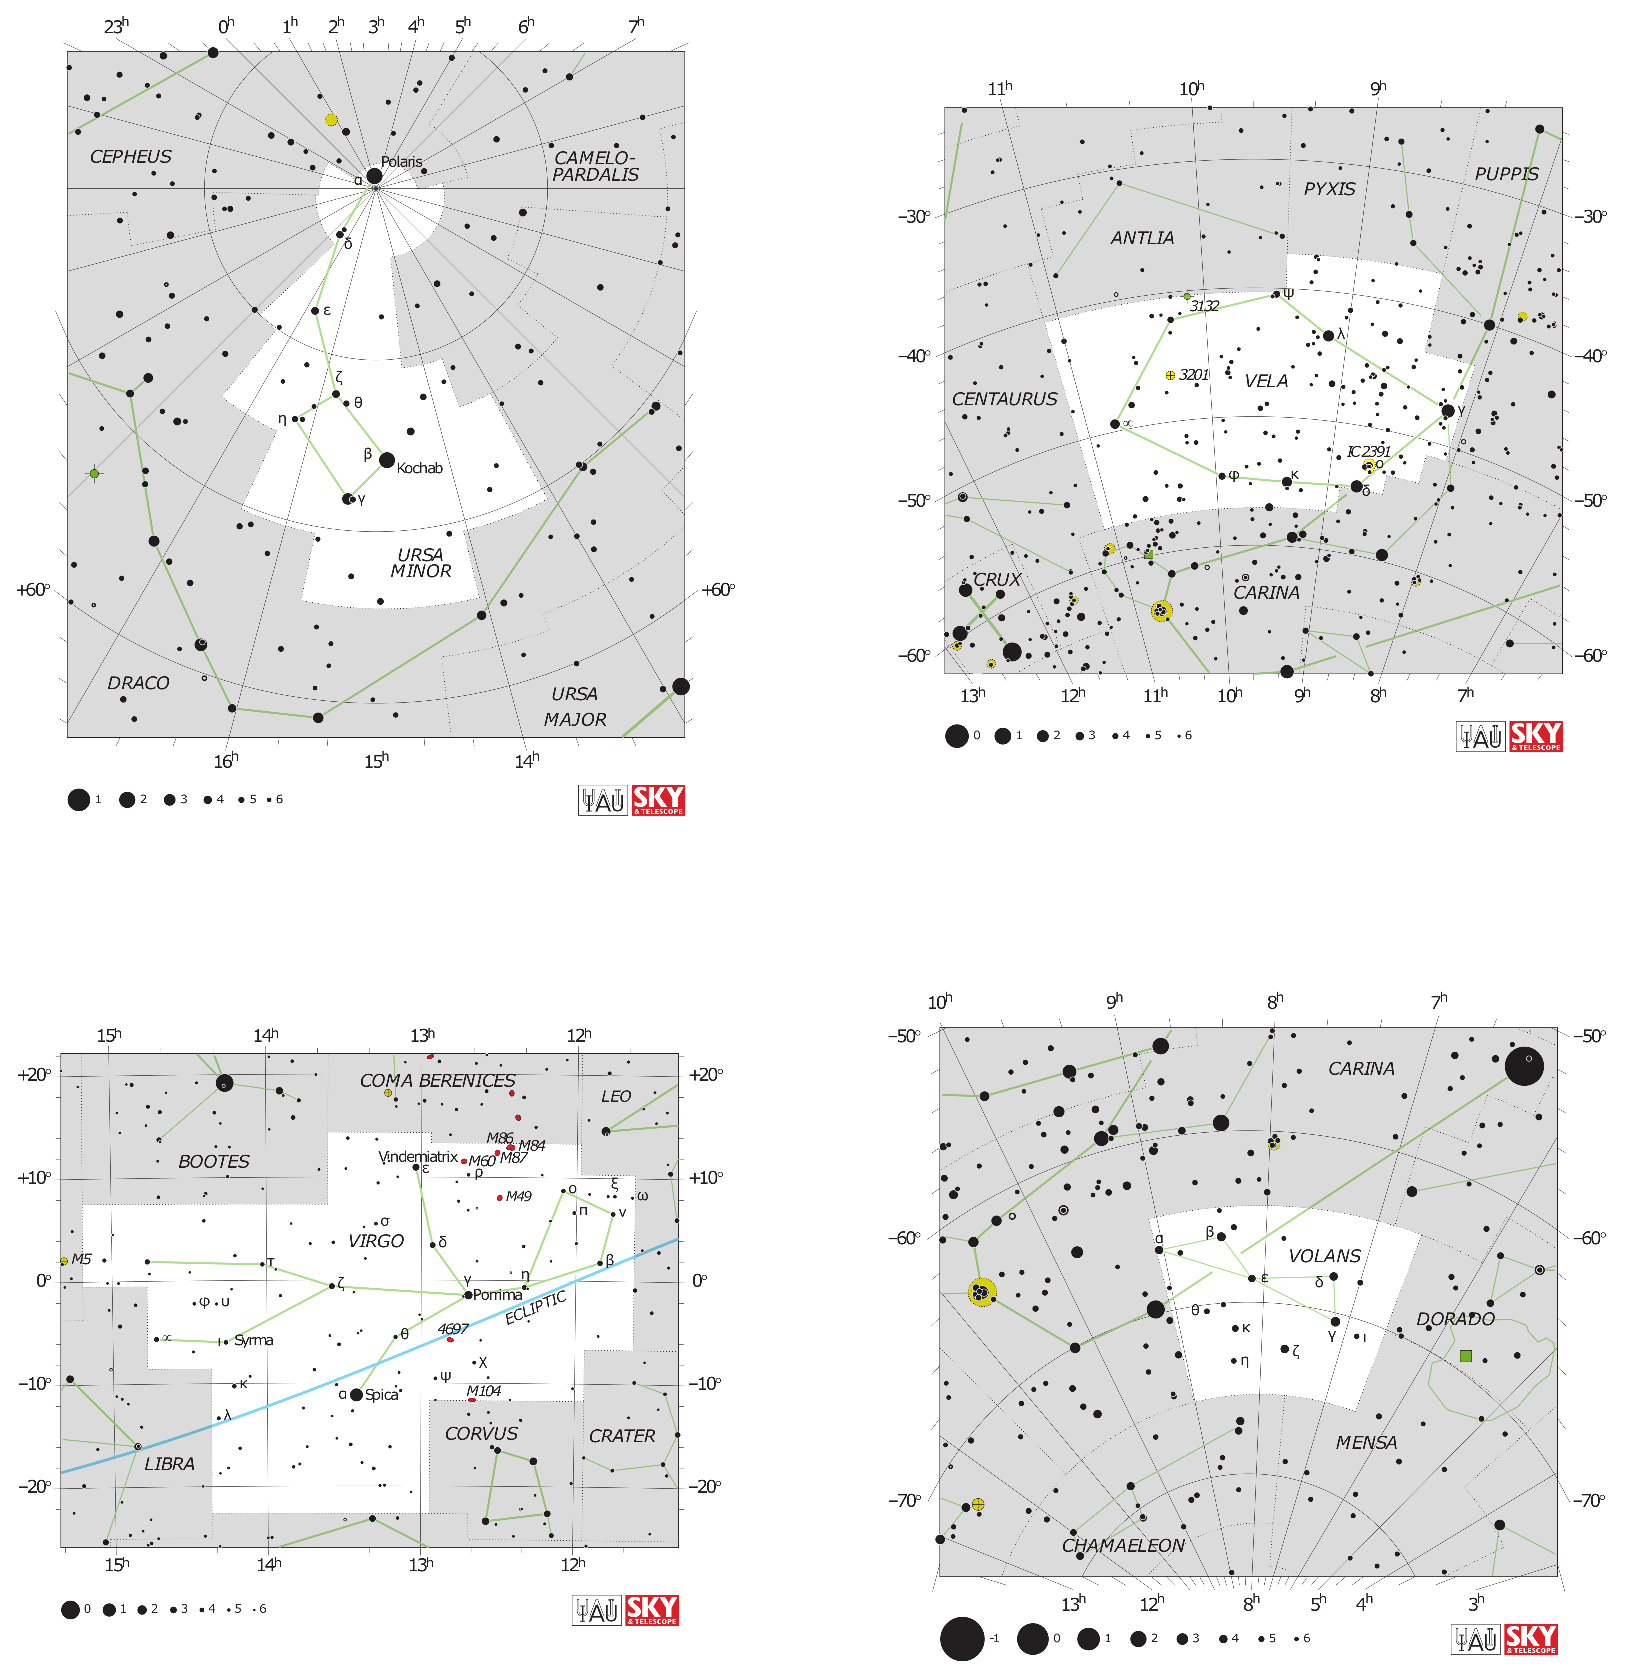
\includegraphics[width=\linewidth]{C22.eps}
\end{figure}
\clearpage
\begin{figure}[H]
	\centering
	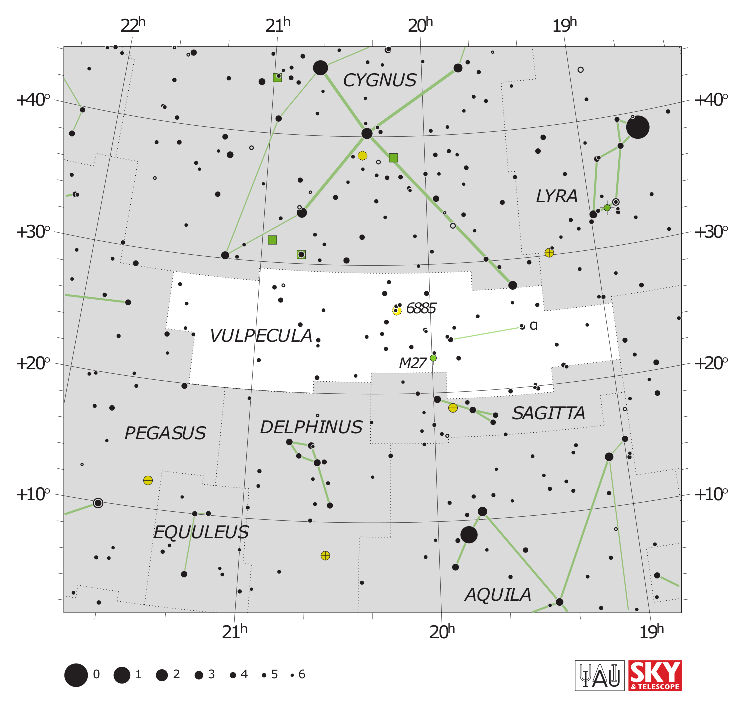
\includegraphics[width=0.5\linewidth]{C23.eps}
\end{figure}
\vspace{1.5cm}
After printing use these constellation images to practice DSOs, planet positions, and angular sizes of a particular projection. Trust me it'll be helpful! A cartoon may describe it like--
\begin{figure}[H]
	\centering
	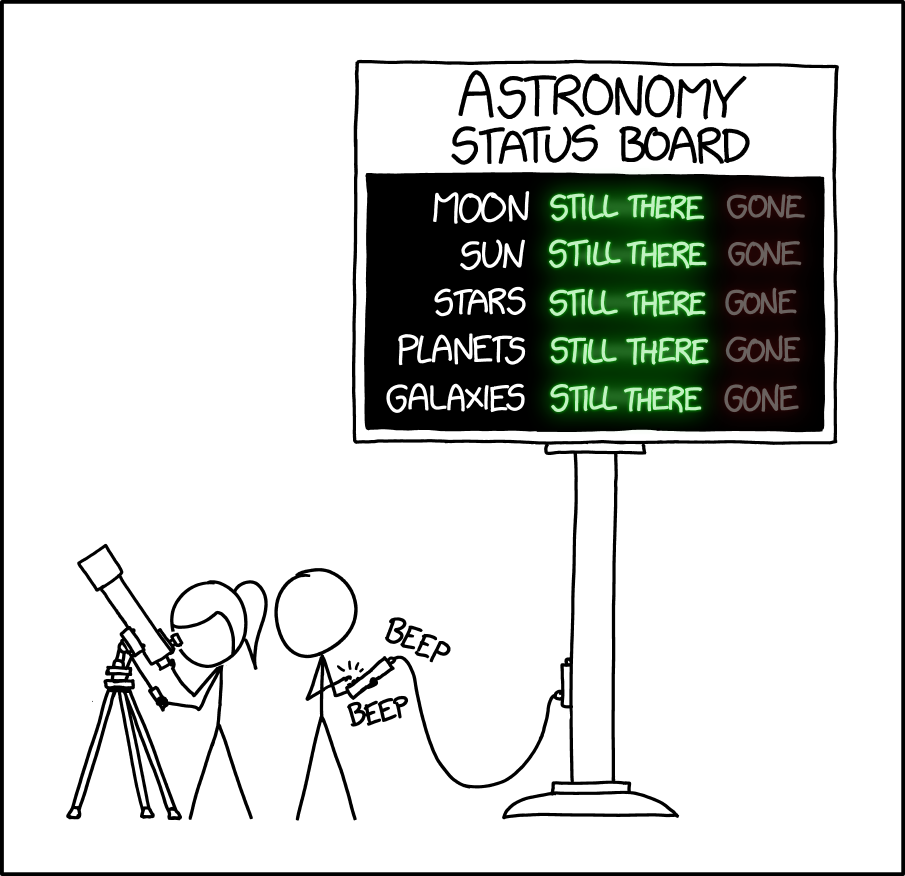
\includegraphics[width=0.5\linewidth]{statusb.png}
\end{figure}
\clearpage
\section{Exploring the Moon}
The Moon is by far the most rewarding celestial object for a small telescope. Even a very small instrument will reveal its bleak, blasted landscape of mountain ranges, plains, hills, valleys, and craters. Even binoculars show many features, and there are enough interesting sites on the Moon to keep a telescopic explorer busy forever.



\begin{figure}[H]
	\centering
	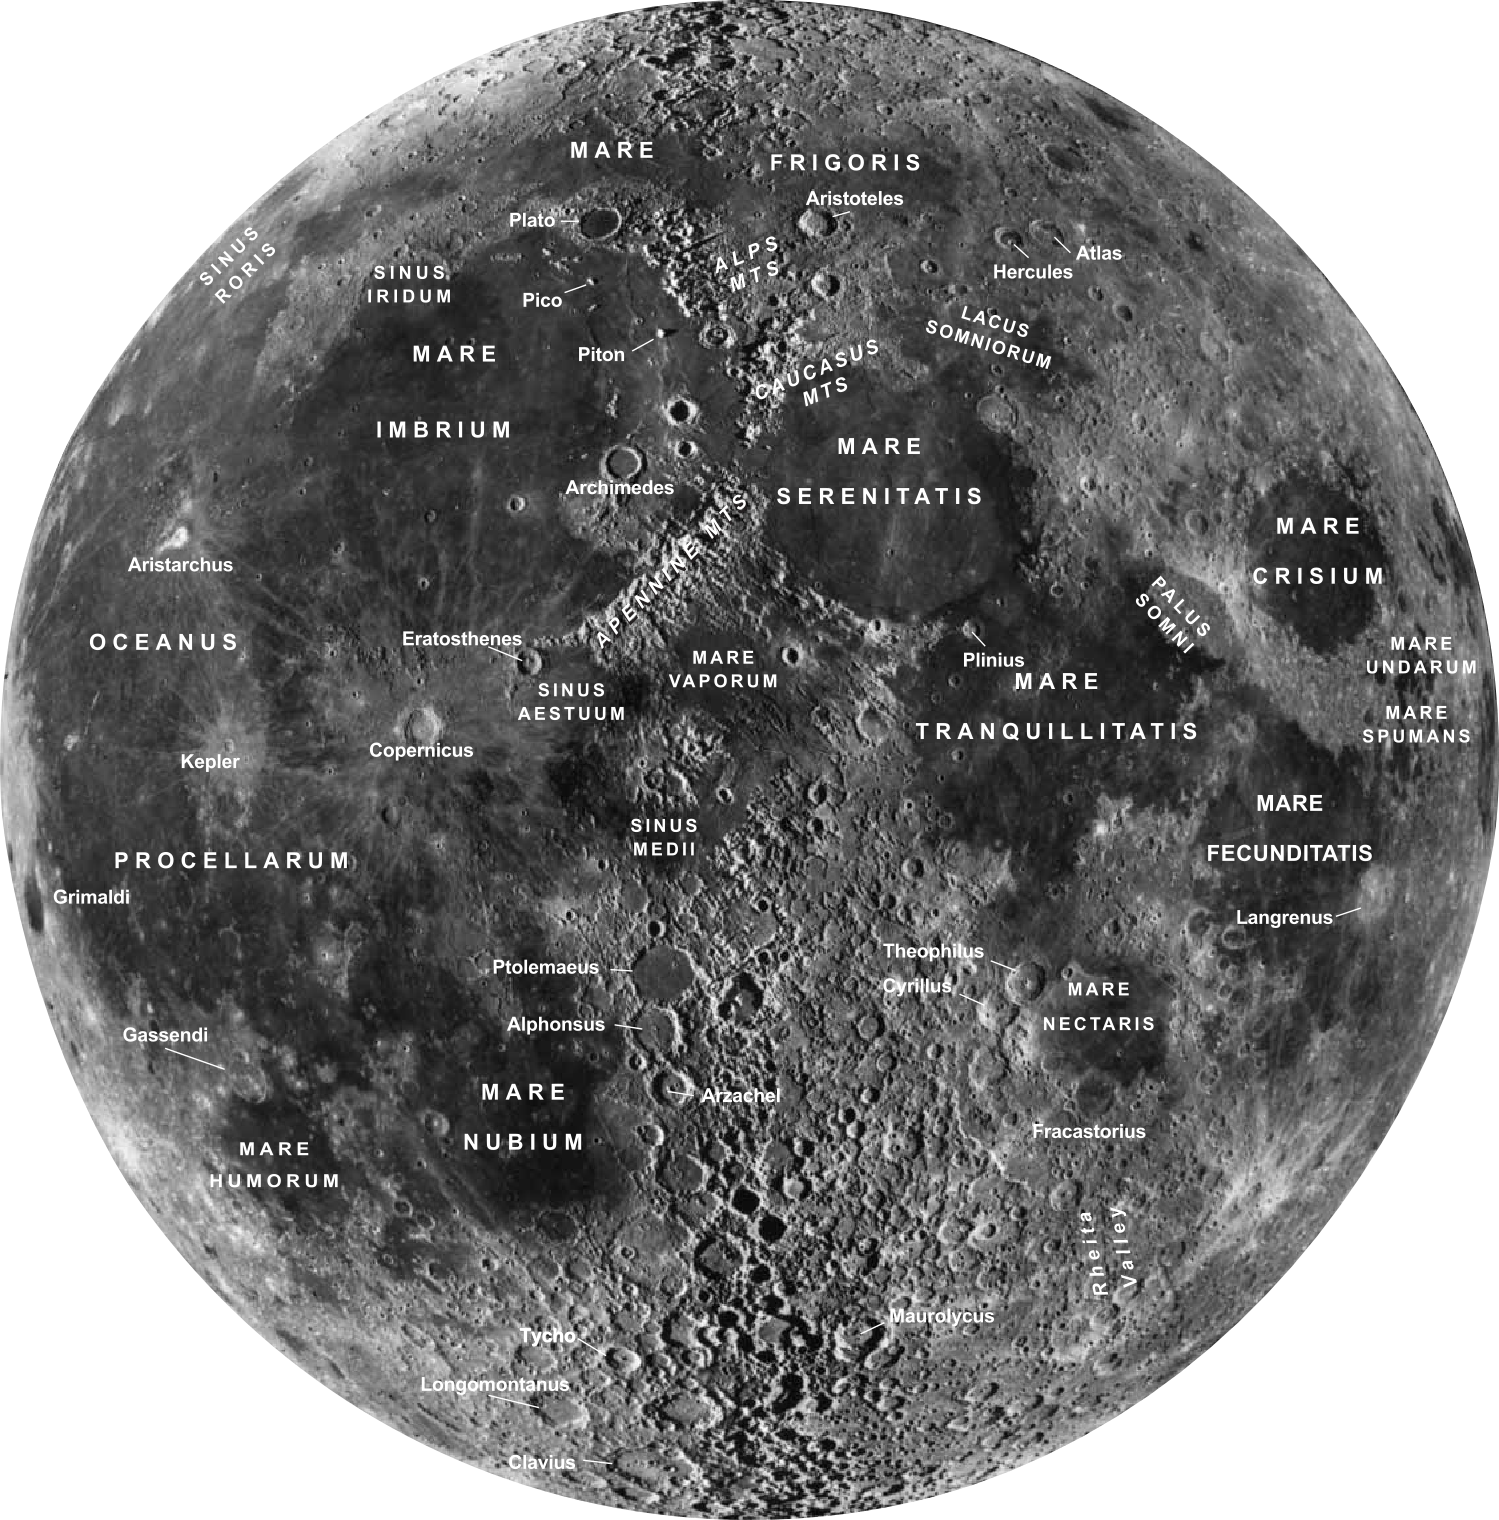
\includegraphics[width=0.9\linewidth]{moon1.png}
\end{figure}
You'll notice right away that except when the Moon is full, it is divided by the terminator, the line separating lunar day and night. Here is where detail shows best. When the Moon is a waxing (growing) crescent, we see the parts on the right edge of the map. At first-quarter phase we see the entire right half, and so on. To use this lunar map, turn the chart until it matches your view. Note: Some telescopes give a mirror image, which will not match this map no matter how you turn it.\\

Refractors and Cassegrain reflectors give mirror images when used with a star diagonal; so does any other instrument containing an odd number of mirrors. If you find this to be a problem, take out the star diagonal and view ``straight through." A correct image is much easier to compare with any map.\\

Once the map is oriented, it will be simple to identify the major craters, mountains, and other features. In time, the geography of this alien world will become as familiar to you as that of our own.

\subsection{Problem: Moon features }
\begin{enumerate}
	\item Match the selenographic objects numbered in the photo and their names and complete the table. Some of the designations of selenographic objects in the list superfluous.
	\item Estimate the angular and linear size of the lunar sea No 4, as well as its area (in km$^2$).
	\item Mark the Moon's poles with signs • and label them with N (North) and S (South).
	\item Mark the landing site for the Apollo 17 mission with an x. Selenographic coordinates this point: $20.2^\circ$ N. lat., $30.8^\circ$ E.
\end{enumerate}
\begin{figure}[H]
	\centering
	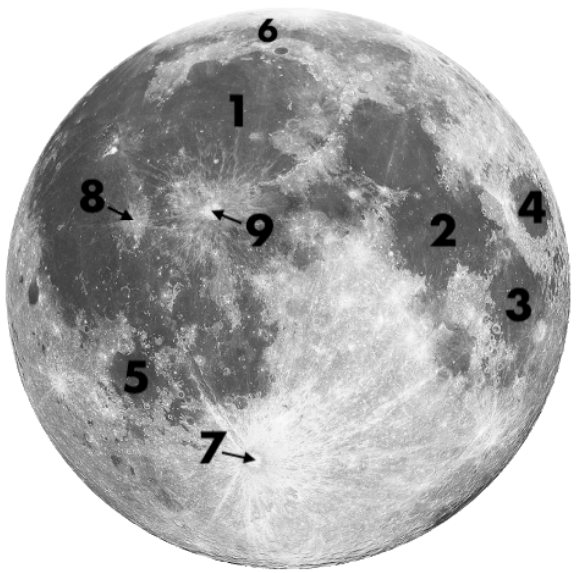
\includegraphics[width=0.8\linewidth]{moon2.png}
\end{figure}


\begin{table}[H]
	\centering
	\begin{tabular}{|l|l|l|l|l|l|lll}
		\cline{1-6}
		Sea (mare)        & No\quad & Sea       & No\quad & Crater       & No &                       &                              &                            \\ \cline{1-6} \cline{8-9} 
		Vaporum      &    & Nectaris    &    & Aristotle    &    & \multicolumn{1}{l|}{} & \multicolumn{1}{l|}{Size}    & \multicolumn{1}{l|}{Answer} \\ \cline{1-6} \cline{8-9} 
		Tranquility &    & Homorum  &    & Kepler       &    & \multicolumn{1}{l|}{} & \multicolumn{1}{l|}{Angular} & \multicolumn{1}{l|}{}      \\ \cline{1-6} \cline{8-9} 
		Clarity     &    & Fecunditatis &    & Copernicus   &    & \multicolumn{1}{l|}{} & \multicolumn{1}{l|}{Linear}  & \multicolumn{1}{l|}{}      \\ \cline{1-6} \cline{8-9} 
		Frigoris        &    & Imbrium    &    & Tycho        &    & \multicolumn{1}{l|}{} & \multicolumn{1}{l|}{Area}    & \multicolumn{1}{l|}{}      \\ \cline{1-6} \cline{8-9} 
		Crisium      &    & Nubium    &    & Eratosthenes &    &                       &                              &                            \\ \cline{1-6}
	\end{tabular}
\end{table}

\textbf{Word Meaning} Vaporum= Vapour (Steam), Frigoris = Cold, Crisium= Crises,Nectaris = Nectar, Homorum = Moisture, Fecunditatis = Ferticility, Imbrium = Rain, Nubium = Clouds. 

\clearpage 
\section{Deep Sky Objects}

\textbf{Deep Sky Objects} shortly DSOs are another interesting element of night sky observation as well as Observation round. Deep sky objects can galaxies, star clusters both open and globular or nebula. It is important to know which what and their perspective position in sky. So it is no wonder that someone has already classified these objects in night sky. The one classification now Astronomers widely follow is done by the French astronomer Charles Messier in his Catalogue des Nébuleuses et des Amas d'Étoiles (Catalogue of Nebulae and Star Clusters). Because Messier was only interested in finding comets, he created a list of those non-comet objects that frustrated his hunt for them. The compilation of this list, in collaboration with his assistant Pierre Méchain, is known as the Messier catalogue. This catalogue of objects is one of the most famous lists of astronomical objects, and many Messier objects are still referenced by their Messier number. You can find 3 kinds of catalogue  on the star map-- Messier Catalogue (M), New General Catalogue (NGC), Index Catalogue (IC)\\

For Olympiad a student must know the position and type of some DSOs. Here are some of these that I recommend---\\

\textbf{Most Important}: {\color{red} 1, 8, 13, 15, 20, 27, 31, 33, 41, 42, 44, 45, 51, 57, 63, 64, 81, 82, 101, 102, 104.}\\

\textbf{Important}: 6, 7, 11, 16, 17, 18, 22, 40, 43, 67, 74, 76, 78, 83, 94, 97.\\

It is not customary to also remember how a particular DSO looks. But for the fascination of these and to know the structure some examples should be remembered which are very popular. For instance Andromeda galaxy, Pleiades or Ring Nebula. In 2018, \nth{12} and 2022, \nth{15} IOAA recognizing DSOs by their image was a controversial question. So I'll suggest, \textit{Be safe than sorry}!  

\begin{figure}[H]
    \centering
    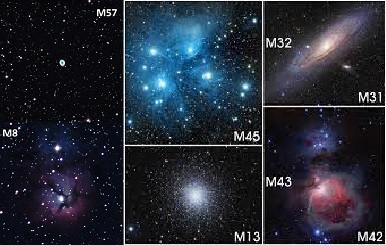
\includegraphics[width=0.5\linewidth]{m_o.jpg}
\end{figure}

In the next page the complete list Messier Objects is given. 


\clearpage
\begin{table}[H]
\tiny
\centering
\caption{\large Messier Object List}
\label{Messier_list}
\begin{tabular}{cccccccc}
\rowcolor[HTML]{EFEFEF} 
{\color[HTML]{000000} \textbf{Messier}} & {\color[HTML]{000000} \textbf{English Name}}                      & {\color[HTML]{000000} \textbf{Constellation}} & {\color[HTML]{000000} \textbf{Status}} & {\color[HTML]{000000} \textbf{\begin{tabular}[c]{@{}c@{}}Apparent \\ Magnitude\end{tabular}}} & {\color[HTML]{000000} \textbf{\begin{tabular}[c]{@{}c@{}}Arc Size \\ (In Minute)\end{tabular}}} & {\color[HTML]{000000} \textbf{\begin{tabular}[c]{@{}c@{}}Minimum \\ Aperture\end{tabular}}} & {\color[HTML]{000000} \textbf{\begin{tabular}[c]{@{}c@{}}Coordinates\\ Dec/RA\end{tabular}}} \\
\rowcolor[HTML]{FFFFFF} 
\textbf{M1}                              & Crab Nebula                                                       & Taurus                                        & Supernova Remnant                      & 8.4                                                                                             & $6\times4$                                                                                              & 50 mm                                                                                       & $+22^\circ 00'/ 05^h 34^m$                                                                   \\
\rowcolor[HTML]{FFF2CC} 
\textbf{M2}                              & \multicolumn{1}{l}{\cellcolor[HTML]{FFF2CC}}                      & Aquarius                                      & Globular Cluster                       & 6.3                                                                                           & 13                                                                                              & Naked Eye                                                                                   & $-00^\circ 49'/ 21^h 33^m$                                                                   \\
\rowcolor[HTML]{FFF2CC} 
\textbf{M3}                              & \multicolumn{1}{l}{\cellcolor[HTML]{FFF2CC}}                      & Canes Venatici                                & Globular Cluster                       & 6.2                                                                                           & 16                                                                                              & Naked Eye                                                                                   & $+28^\circ 22'/ 13^h 42^m$                                                                   \\
\rowcolor[HTML]{FFF2CC} 
\textbf{M4}                              & \multicolumn{1}{l}{\cellcolor[HTML]{FFF2CC}}                      & Scorpius                                      & Globular Cluster                       & 5.9                                                                                           & 26                                                                                              & 15 mm                                                                                       & $-26^\circ 31'/ 16^h 23^m$                                                                   \\
\rowcolor[HTML]{FFF2CC} 
\textbf{M5}                              & \multicolumn{1}{l}{\cellcolor[HTML]{FFF2CC}}                      & Serpens                                       & Globular Cluster                       & 6.7                                                                                           & 17                                                                                              & Naked Eye                                                                                   & $+02^ 04'/ 15^h 18^m $                                                                       \\
\rowcolor[HTML]{D9EAD3} 
\textbf{M6}                              & Butterfly Cluster                                                 & Scorpius                                      & Open Cluster                           & 4.2                                                                                           & 15                                                                                              & Naked Eye                                                                                   & $-32^\circ 13'/ 17^h 40.1^m$                                                                 \\
\rowcolor[HTML]{D9EAD3} 
\textbf{M7}                              & Ptolemy Cluster                                                   & Scorpius                                      & Open Cluster                           & 3.3                                                                                           & 80                                                                                              & Naked Eye                                                                                   & $-34^\circ 47'/ 7^h 53^m$                                                                    \\
\rowcolor[HTML]{E6B8AF} 
\textbf{M8}                              & Lagoon Nebula                                                     & Sagittarius                                   & Diffuse Nebula                         & 6                                                                                             & $90 \times 40$                                                                                  & Naked Eye                                                                                   & $-24^\circ 23'/ 18^h 03^m$                                                                   \\
\rowcolor[HTML]{FFF2CC} 
\textbf{M9}                              & \multicolumn{1}{l}{\cellcolor[HTML]{FFF2CC}}                      & Ophiuchus                                     & Globular Cluster                       & 8.4                                                                                           & 9                                                                                               & 30 mm                                                                                       & $-18^\circ 30'/ 17^h 19^m$                                                                   \\
\rowcolor[HTML]{FFF2CC} 
\textbf{M10}                             & \multicolumn{1}{l}{\cellcolor[HTML]{FFF2CC}}                      & Ophiuchus                                     & Globular Cluster                       & 6.4                                                                                           & 15                                                                                              & Naked Eye                                                                                   & $-04^\circ 05'/ 16^h 57^m$                                                                   \\
\rowcolor[HTML]{D9EAD3} 
\textbf{M11}                             & Wild Duck Cluster                                                 & Scutum                                        & Open Cluster                           & 6.3                                                                                           & 14                                                                                              & Naked Eye                                                                                   & $-06^\circ 16'/ 18^h 51.1^m$                                                                 \\
\rowcolor[HTML]{FFF2CC} 
\textbf{M12}                             & \multicolumn{1}{l}{\cellcolor[HTML]{FFF2CC}}                      & Ophiuchus                                     & Globular Cluster                       & 7.7                                                                                           & 15                                                                                              & 15 mm                                                                                       & $-01^\circ 56'/ 16^h 47^m$                                                                   \\
\rowcolor[HTML]{FFF2CC} 
\textbf{M13}                             & \begin{tabular}[c]{@{}c@{}}Great Hercules \\ Cluster\end{tabular} & Hercules                                      & Globular Cluster                       & 5.8                                                                                           & 17                                                                                              & Naked Eye                                                                                   & $+36^\circ 27'/ 16^h 41^m$                                                                   \\
\rowcolor[HTML]{FFF2CC} 
\textbf{M14}                             & \multicolumn{1}{l}{\cellcolor[HTML]{FFF2CC}}                      & Ophiuchus                                     & Globular Cluster                       & 8.3                                                                                           & 12                                                                                              & 30 mm                                                                                       & $-03^\circ 14'/ 17^h 37^m$                                                                   \\
\rowcolor[HTML]{FFF2CC} 
\textbf{M15}                             & \begin{tabular}[c]{@{}c@{}}Great Pegasus \\ Cluster\end{tabular}  & Pegasus                                       & Globular Cluster                       & 6.2                                                                                           & 12                                                                                              & Naked Eye                                                                                   & $+12^\circ 10'/ 21^h 29^m$                                                                   \\
\rowcolor[HTML]{D9D2E9} 
\textbf{M16}                             & Eagle Nebula                                                      & Serpens                                       & Stellar Nebula                         & 7                                                                                             & 7                                                                                               & Naked Eye                                                                                   & $-13^\circ 49'/ 18^h 18^m$                                                                   \\
\rowcolor[HTML]{D9D2E9} 
\textbf{M17}                             & Omega Nebula                                                      & Sagittarius                                   & Stellar Nebula                         & 6                                                                                             & $46\times37$                                                                                    & 30 mm                                                                                       & $-16^\circ 10'/ 18^h 20^m$                                                                   \\
\rowcolor[HTML]{D9EAD3} 
\textbf{M18}                             & Swan                                                              & Sagittarius                                   & Open Cluster                           & 7.5                                                                                          & 9                                                                                               & 15 mm                                                                                       & $-17^\circ 08'/ 18^h 19.9^m$                                                                 \\
\rowcolor[HTML]{FFF2CC} 
\textbf{M19}                             & \multicolumn{1}{l}{\cellcolor[HTML]{FFF2CC}}                      & Ophiuchus                                     & Globular Cluster                       & 7.5                                                                                           & 14                                                                                              & 30 mm                                                                                       & $-26^\circ 16'/ 17^h 02^m$                                                                   \\
\rowcolor[HTML]{E6B8AF} 
\textbf{M20}                             & Trifid Nebula                                                     & Sagittarius                                   & Diffuse Nebula                         & 6.3                                                                                             & $28\times 28$                                                                                   & 30 mm                                                                                       & $-23^\circ 01'/ 18^h 02^m $          \\
\rowcolor[HTML]{D9EAD3} 
\textbf{M21} &                                                                    & Sagittarius & Open Cluster      & 6.5 & 13    & 15 mm     & $-22^\circ 30' / 18^h 04.6^m$        \\
\rowcolor[HTML]{FFF2CC} 
\textbf{M22} & \multicolumn{1}{c}{\cellcolor[HTML]{FFF2CC}Sagittarius Cluster}    & Sagittarius & Globular Cluster  & 5.1 & 24    & Naked Eye & $-23^\circ 54'/ 18^h 36^m$           \\
\rowcolor[HTML]{D9EAD3} 
\textbf{M23} &                                                                    & Sagittarius & Open Cluster      & 6.9   & 27    & Naked Eye & $-19^\circ 01'/ 17^h 56.8^m$         \\
\rowcolor[HTML]{FFFFFF} 
\textbf{M24} & \multicolumn{1}{c}{\cellcolor[HTML]{FFFFFF}Sagittarius Star Cloud} & Sagittarius & Star Cloud        & 2.5 & $90\times 60$  & Naked Eye & $-18^\circ 29' / 18^h 17^m$          \\
\rowcolor[HTML]{D9EAD3} 
\textbf{M25} &                                                                    & Sagittarius & Open Cluster      & 4.6 & 32    & Naked Eye & $-19^\circ 15'/ 18^h 31.6^m$         \\
\rowcolor[HTML]{D9EAD3} 
\textbf{M26} &                                                                    & Scutum      & Open Cluster      & 8   & 15    & 50 mm     & $-09^\circ 24' / 18^h 45.2^m$        \\
\rowcolor[HTML]{D0E0E3} 
\textbf{M27} & \multicolumn{1}{c}{\cellcolor[HTML]{D0E0E3}Dumbbell Nebula}        & Vulpecula   & Planetary Nebula  & 7.5   & $8\times6$    & 30 mm     & $+22^\circ 43'/ 19^h 59^m$           \\
\rowcolor[HTML]{FFF2CC} 
\textbf{M28} &                                                                    & Sagittarius & Globular Cluster  & 7.7 & 11    & 30 mm     & $-24^\circ 52'/ 18^h 24^m$           \\
\rowcolor[HTML]{D9EAD3} 
\textbf{M29} &    Cooling Tower                                                                & Cygnus      & Open Cluster      & 7.1 & 7     & Naked Eye & $+38^\circ 31'/ 20^h 23^m$           \\
\rowcolor[HTML]{FFF2CC} 
\textbf{M30} &                                                                    & Capricornus & Globular Cluster  & 7.7 & 11    & 30 mm     & $-23^\circ 10'/ 21^h 40^m$           \\
\rowcolor[HTML]{00FFFF} 
\textbf{M31} & \multicolumn{1}{c}{\cellcolor[HTML]{00FFFF}Andromeda Galaxy}       & Andromeda   & Spiral Galaxy     & 3.4 & $190.2\times 60$ & Naked Eye & $+41^\circ 16'9''/ 00^h 42^m$ \\
\rowcolor[HTML]{F3F3F3} 
\textbf{M32} &                                                                    & Andromeda   & Elliptical Galaxy & 8.1 & $8\times6$    & 30 mm     & $+40^\circ51'/ 00^h 42^m$            \\
\rowcolor[HTML]{00FFFF} 
\textbf{M33} & \multicolumn{1}{c}{\cellcolor[HTML]{00FFFF}Triangulum Galaxy}      & Triangulum  & Spiral Galaxy     & 5.7 & $70.8\times 41.7$  & Naked Eye & $+30^\circ 39'/ 01^h 33^m$           \\
\rowcolor[HTML]{D9EAD3} 
\textbf{M34} &                                                                    & Perseus     & Open Cluster      & 5.2 & 35    & Naked Eye & $+42^\circ 46'/ 02^h 42.1^m$         \\
\rowcolor[HTML]{D9EAD3} 
\textbf{M35} &                                                                    & Gemini      & Open Cluster      & 5.5 & 28    & Naked Eye & $+24^\circ 21'/ 06^h 09.1^m$         \\
\rowcolor[HTML]{D9EAD3} 
\textbf{M36} &                                                                    & Auriga      & Open Cluster      & 6.3   & 12    & Naked Eye & $+34^\circ 08'/ 05^h 36^m$           \\
\rowcolor[HTML]{D9EAD3} 
\textbf{M37} &                                                                    & Auriga      & Open Cluster      & 6.2 & 24    & Naked Eye & $+32^\circ 33'/ 05^h 52^m$           \\
\rowcolor[HTML]{D9EAD3} 
\textbf{M38} &     Starfish Cluster                                                               & Auriga      & Open Cluster      & 7..4 & 21    & Naked Eye & $+35^\circ 51'/ 05^h 28^m $          \\
\rowcolor[HTML]{D9EAD3} 
\textbf{M39} &                                                                    & Cygnus      & Open Cluster      & 5.5 & 32    & Naked Eye & $+48^\circ 26'/ 21^h 31^m$           \\
\textbf{M40} & \multicolumn{1}{c}{Winnecke 4}                                     & Ursa Major  & Double Star       & 9.7 & 1     & 50 mm     & $+58^\circ 4'/ 12^h 22^m$            \\
\rowcolor[HTML]{D9EAD3} 
\textbf{M41} & \multicolumn{1}{c}{\cellcolor[HTML]{D9EAD3}Little Beehive}         & Canis Major & Open Cluster      & 4.5 & 38    & Naked Eye & $-20^\circ 46'/ 06^h 46.0^m$         \\
\rowcolor[HTML]{E6B8AF} 
\textbf{M42} & \multicolumn{1}{c}{\cellcolor[HTML]{E6B8AF}Orion Nebula}           & Orion       & Diffuse Nebula    & 4   & $65\times 60$  & Naked Eye & $-05^\circ 23'/ 05^h 35^m$           \\
\rowcolor[HTML]{E6B8AF} 
\textbf{M43} & \multicolumn{1}{c}{\cellcolor[HTML]{E6B8AF}De  Mairan’s Nebula}    & Orion       & Diffuse Nebula    & 9   & $20\times 15$  & 50 mm     & $-05^\circ 16'/ 05^h 35^m$           \\
\rowcolor[HTML]{D9EAD3} 
\textbf{M44} & \multicolumn{1}{c}{\cellcolor[HTML]{D9EAD3}Praesepe /Beehive}      & Cancer      & Open Cluster      & 3.7 & 95    & Naked Eye & $+19^\circ 59'/ 08^h 40.4^m$         \\
\rowcolor[HTML]{D9EAD3} 
\textbf{M45} & \multicolumn{1}{c}{\cellcolor[HTML]{D9EAD3}Pleiades}               & Taurus      & Open Cluster      & 1.6 & 110   & Naked Eye & $+24^\circ 07'/ 03^h 47^m$     \\
\rowcolor[HTML]{D9EAD3} 
\textbf{M46} &                                                              & Puppis         & Open Cluster      & 6.1 & 27  & Naked Eye & $-14^\circ 49'/ 07^h 41.8^m$    \\
\rowcolor[HTML]{D9EAD3} 
\textbf{M47} &                                                              & Puppis         & Open Cluster      & 4.2 & 30  & Naked Eye & $-14^\circ 30'/ 07^h 36.6^m$    \\
\rowcolor[HTML]{D9EAD3} 
\textbf{M48} &                                                              & Hydra          & Open Cluster      & 5.5 & 54  & Naked Eye & $-05^\circ 45'/ 08^h 13.7^m$    \\
\rowcolor[HTML]{F3F3F3} 
\textbf{M49} &                                                              & Virgo          & Elliptical Galaxy & 9.4 & 97  & 50 mm     & $+08^\circ 00'/ 12^h 29^m$      \\
\rowcolor[HTML]{D9EAD3} 
\textbf{M50} &                                                              & Monoceros      & Open Cluster      & 5.9 & 16  & Naked Eye & $-08^\circ 20'/ 07^h 03.2^m$    \\
\rowcolor[HTML]{00FFFF} 
\textbf{M51} & \multicolumn{1}{c}{\cellcolor[HTML]{00FFFF}Whirlpool Galaxy} & Canes Venatici & Spiral Galaxy     & 8.4 & $11\times8$ & 50 mm     & $+47^\circ 11'/ 13^h 29^m $     \\
\rowcolor[HTML]{D9EAD3} 
\textbf{M52} &                                                              & Cassiopeia     & Open Cluster      & 5 & 13  & 30 mm     & $+61^\circ 35'/ 23^h 24.2^m$    \\
\rowcolor[HTML]{FFF2CC} 
\textbf{M53} &                                                              & Coma Berenices & Globular Cluster  & 8.3 & 13  & 30 mm     & $+18^\circ 10'/ 13^h 12^m $     \\
\rowcolor[HTML]{FFF2CC} 
\textbf{M54} &                                                              & Sagittarius    & Globular Cluster  & 8.4 & 9   & 50 mm     & $-30^\circ 28'/ 18^h 55^m $     \\
\rowcolor[HTML]{FFF2CC} 
\textbf{M55} &                                                              & Sagittarius    & Globular Cluster  & 7.4 & 19  & Naked Eye & $30^\circ 57'/ 19^h 39^m $      \\
\rowcolor[HTML]{FFF2CC} 
\textbf{M56} &                                                              & Lyra           & Globular Cluster  & 8.3 & 7   & 50 mm     & $+30^\circ 11'/ 19^h 16^m$      \\
\rowcolor[HTML]{D0E0E3} 
\textbf{M57} & \multicolumn{1}{c}{\cellcolor[HTML]{D0E0E3}Ring Nebula}      & Lyra           & Planetary Nebula  & 8.8 & 1.3 & 50 mm     & $+33^\circ 01'/ 18^h 53^m $     \\
\rowcolor[HTML]{00FFFF} 
\textbf{M58} &                                                              & Virgo          & Spiral Galaxy     & 10.5 & $5\times4$  & 50 mm     & $+11^\circ 49'/ 12^h 37^m $     \\
\rowcolor[HTML]{F3F3F3} 
\textbf{M59} &                                                              & Virgo          & Elliptical Galaxy & 10.6 & $5\times3$  & 50 mm     & $+11^\circ 38' 49''/ 12^h 42^m$ \\
\rowcolor[HTML]{F3F3F3} 
\textbf{M60} &                                                              & Virgo          & Elliptical Galaxy & 9.8 & $7\times6$  & 50 mm     & $+11^\circ 33'/ 12^h 43^m$     \\
\rowcolor[HTML]{00FFFF} 
\textbf{M61} &                                                              & Virgo          & Spiral Galaxy    & 10.2 & $6\times5$  & 50 mm                                        & $+04^\circ 28'/ 12^h 21^m$   \\
\rowcolor[HTML]{FFF2CC} 
\textbf{M62} &                                                              & Ophiuchus      & Globular Cluster & 7.4 & 14  & 15 mm                                        & $-30^\circ 06'/ 17^h 01^m$   \\
\rowcolor[HTML]{00FFFF} 
\textbf{M63} & \multicolumn{1}{c}{\cellcolor[HTML]{00FFFF}Sunflower Galaxy} & Canes Venatici & Spiral Galaxy    & 9.3 & $12\times 8$ & 30 mm                                        & $+42^\circ 01'/ 13^h 15^m$   \\
\rowcolor[HTML]{00FFFF} 
\textbf{M64} & \multicolumn{1}{c}{\cellcolor[HTML]{00FFFF}Black Eye Galaxy} & Coma Berenices & Spiral Galaxy    & 9.4 & $9\times5$  & 50 mm                                        & $+21^\circ 40'/ 12^h 56^m$   \\
\rowcolor[HTML]{00FFFF} 
\textbf{M65} &      Leo Triplet                                                        & Leo            & Spiral Galaxy    & 10.3 & $10\times3$ & 30 mm                                        & $+13^\circ 05'/ 11^h 18^m$   \\
\rowcolor[HTML]{00FFFF} 
\textbf{M66} &        Leo Triplet                                                      & Leo            & Spiral Galaxy    & 8.9 & $9\times4$  & 30 mm                                        & $+12^\circ 59'/ 11^h 20^m$   \\
\rowcolor[HTML]{D9EAD3} 
\textbf{M67} & \multicolumn{1}{c}{\cellcolor[HTML]{D9EAD3}King Cobra}       & Cancer         & Open Cluster     & 6.1 & 30  & \multicolumn{1}{l}{\cellcolor[HTML]{D9EAD3}} & $+11^\circ 49'/ 08^h 51.3^m$ \\
\rowcolor[HTML]{FFF2CC} 
\textbf{M68} &                                                              & Hydra          & Globular Cluster & 9.7 & 12  & 50 mm                                        & $-26^\circ 44'/ 12^h 39^m$   \\
\rowcolor[HTML]{FFF2CC} 
\textbf{M69} &                                                              & Sagittarius    & Globular Cluster & 8.3 & 7   & 50 mm                                        & $-32^\circ 20'/ 18^h 31^m$   \\
\rowcolor[HTML]{FFF2CC} 
\textbf{M70} &                                                              & Sagittarius    & Globular Cluster & 9.1 & 8   & 50 mm                                        & $-32^\circ 17'/ 18^h 43^m$   \\
\rowcolor[HTML]{FFF2CC} 
\textbf{M71} &                                                              & Sagitta        & Globular Cluster & 6.1 & 7   & 50 mm                                        & $+18^\circ 46'/ 19^h 53^m$  \\
\rowcolor[HTML]{FFF2CC} 
\textbf{M72} &                                                                                                               & Aquarius    & Globular Cluster & 9.4  & 6   & 50 mm & $-12^\circ 32'/ 20^h 53^m$      \\
\textbf{M73} &                                                                                                               & Aquarius    & Asterism         & 9 & 1   & 50 mm & $-12^\circ 38'/ 20^h 58^m 54^s$ \\
\rowcolor[HTML]{00FFFF} 
\textbf{M74} & \multicolumn{1}{c}{\cellcolor[HTML]{00FFFF}The Phantom}                                                       & Pisces      & Spiral Galaxy    & 10 & $10\times9$ & 50 mm & $+15^\circ 47'/  01^h 36^m$     \\
\rowcolor[HTML]{FFF2CC} 
\textbf{M75} &                                                                                                               & Sagittarius & Globular Cluster & 9.2  & 6   & 50 mm & $-21^\circ 55'/ 20^h 06^m$      \\
\rowcolor[HTML]{D0E0E3} 
\textbf{M76} & \multicolumn{1}{c}{\cellcolor[HTML]{D0E0E3}\begin{tabular}[c]{@{}c@{}}Little Dumbbell \\ Nebula\end{tabular}} & Perseus     & Planetary Nebula & 10.1 & $2\times1$  & 50 mm & $+51^\circ 34'/ 01^h 42.4^m$    \\
\rowcolor[HTML]{00FFFF} 
\textbf{M77} & \multicolumn{1}{c}{\cellcolor[HTML]{00FFFF}Cetus A}                                                           & Cetus       & Spiral Galaxy    & 9.6  & $7\times6$  & 50 mm & $-00^\circ 00'/ 02^h 42^m$       
\end{tabular}
\end{table}

\clearpage
\begin{table}[H]
\centering
\tiny 
\begin{tabular}{clcccccc}
\rowcolor[HTML]{EFEFEF} 
{\color[HTML]{000000} \textbf{Messier}} & \multicolumn{1}{c}{\cellcolor[HTML]{EFEFEF}{\color[HTML]{000000} \textbf{English Name}}} & {\color[HTML]{000000} \textbf{Constellation}} & {\color[HTML]{000000} \textbf{Status}} & {\color[HTML]{000000} \textbf{\begin{tabular}[c]{@{}c@{}}Apparent \\ Magnitude\end{tabular}}} & {\color[HTML]{000000} \textbf{\begin{tabular}[c]{@{}c@{}}Arc Size \\ (In Minute)\end{tabular}}} & {\color[HTML]{000000} \textbf{\begin{tabular}[c]{@{}c@{}}Minimum \\ Aperture\end{tabular}}} & {\color[HTML]{000000} \textbf{\begin{tabular}[c]{@{}c@{}}Coordinates\\ Dec/RA\end{tabular}}} \\
\rowcolor[HTML]{E6B8AF} 
\textbf{M78} &                                                                                                               & Orion       & Diffuse Nebula   & 8.3  & $8\times6$  & 50 mm & $+00^\circ 00'/ 05^h 46^m$      \\
\rowcolor[HTML]{FFF2CC} 
\textbf{M79} &                                                                                                               & Lepus       & Globular Cluster & 8.6  & 9   & 50 mm & $-24^\circ 31'/ 05^h 24^m$      \\
\rowcolor[HTML]{FFF2CC} 
\textbf{M80} &                                                                                                               & Scorpius    & Globular Cluster & 7.9  & 9   & 50 mm & $-22^\circ 58'/ 16^h 17^m$    \\
\rowcolor[HTML]{00FFFF} 
\textbf{M81}                             & \multicolumn{1}{c}{\cellcolor[HTML]{00FFFF}Bode’s Galaxy}                                & Ursa Major                                    & Spiral Galaxy                 & 6.9                                                                                           & $26\times14$                                                                                            & Naked Eye                                                                                   & $+69^\circ 3'/ 09^h 55^m$                                                                    \\
\textbf{M82}                             & \multicolumn{1}{c}{Cigar Galaxy}                                                         & Ursa Major                                    & Irregular Galaxy             & 8.4                                                                                           & $11\times5$                                                                                             & 30 mm                                                                                       & $+69^\circ 40'/ 09^h 55^m$                                                                   \\
\rowcolor[HTML]{00FFFF} 
\textbf{M83}                             & \multicolumn{1}{c}{\cellcolor[HTML]{00FFFF}Southern Pinwheel}                            & Hydra                                         & Spiral Galaxy                 & 7.5                                                                                           & $11\times10$                                                                                            & 30 mm                                                                                       & $29^\circ 51'/ 13^h 37^m$                                                                    \\
\rowcolor[HTML]{F3F3F3} 
\textbf{M84}                             &                                                                                          & Virgo                                         & Elliptical Galaxy             & 10.1                                                                                          & $5\times4$                                                                                              & 50 mm                                                                                       & $+12^\circ 53'/ 12^h 25^m$                                                                   \\
\rowcolor[HTML]{F3F3F3} 
\textbf{M85}                             &                                                                                          & Coma Berenices                                & Elliptical Galaxy             & 10                                                                                          & $7\times5$                                                                                              & 50 mm                                                                                       & $+18^\circ 11'/ 12^h 25^m$                                                                   \\
\rowcolor[HTML]{F3F3F3} 
\textbf{M86}                             &                                                                                          & Virgo                                         & Elliptical Galaxy             & 9.8                                                                                           & $7\times5$                                                                                              & 50 mm                                                                                       & $+12^\circ 56'/ 12^h 26^m$                                                                   \\
\rowcolor[HTML]{F3F3F3} 
\textbf{M87}                             &  Virgo A                                                                                        & Virgo                                         & Elliptical Galaxy             & 9.6                                                                                           & 7                                                                                               & 50 mm                                                                                       & $+12^\circ 23'/ 12^h 30^m$                                                                   \\
\rowcolor[HTML]{00FFFF} 
\textbf{M88}                             &                                                                                          & Coma Berenices                                & Spiral Galaxy                & 10.4                                                                                          & $7\times4$                                                                                              & 50 mm                                                                                       & $+14^\circ 25'/ 12^h 31^m$                                                                   \\
\rowcolor[HTML]{F3F3F3} 
\textbf{M89}                             &                                                                                          & Virgo                                         & Elliptical Galaxy             & 10.7                                                                                         & 4                                                                                               & 50 mm                                                                                       & $+12°^\circ 33'/ 12^h 35^m$                                                                  \\
\rowcolor[HTML]{00FFFF} 
\textbf{M90}                             &                                                                                          & Virgo                                         & Spiral Galaxy                & 10.3                                                                                          & $10\times5$                                                                                             & 50 mm                                                                                       & $+13^\circ 09'/ 12^h 36^m$                                                                   \\
\rowcolor[HTML]{00FFFF} 
\textbf{M91}                             &                                                                                          & Coma Berenices                                & Spiral Galaxy                 & 11                                                                                          & $5\times4$                                                                                              & 60 mm                                                                                       & $+14^\circ 29'/ 12^h 35^m$                                                                   \\
\rowcolor[HTML]{FFF2CC} 
\textbf{M92}                             &                                                                                          & Hercules                                      & Globular Cluster              & 6.4                                                                                           & 11                                                                                              & Naked Eye                                                                                   & $+43^\circ 08'/ 17^h 17^m$                                                                   \\
\rowcolor[HTML]{D9EAD3} 
\textbf{M93}                             &                                                                                          & Puppis                                        & Open Cluster                 & 6                                                                                             & 22                                                                                              & 30 mm                                                                                       & $-23^\circ 52'/ 07^h 44.6^m$                                                                 \\
\rowcolor[HTML]{00FFFF} 
\textbf{M94}                             & \multicolumn{1}{c}{\cellcolor[HTML]{00FFFF}Cat’s Eye Galaxy}                             & Canes Venatici                                & Spiral galaxy                & 9                                                                                           & $11\times9$                                                                                             & 30 mm                                                                                       & $+41^\circ 07'/ 12^h 50^m$                                                                   \\
\rowcolor[HTML]{00FFFF} 
\textbf{M95}                             &                                                                                          & Leo                                           & Spiral Galaxy               & 11.4                                                                                           & $7\times5$                                                                                              & 50 mm                                                                                       & $+11^\circ 42'/ 10^h 43^m$                                                                   \\
\rowcolor[HTML]{00FFFF} 
\textbf{M96}                             &                                                                                          & Leo                                           & Spiral Galaxy                 & 10.1                                                                                          & $7\times5$                                                                                              & 50 mm                                                                                       & $+11^\circ 49'/ 10^h 46^m$                                                                   \\
\rowcolor[HTML]{D0E0E3} 
\textbf{M97}                             & \multicolumn{1}{c}{\cellcolor[HTML]{D0E0E3}Owl Nebula}                                   & Ursa Major                                    & Planetary Nebula              & 9.9                                                                                            & 3                                                                                               & 50 mm                                                                                       & $+55^\circ  01'/ 11^h 14^m$ \\
\rowcolor[HTML]{00FFFF} 
\textbf{M98}  &                                                                                                                       & Coma Berenices & Spiral Galaxy     & 11 & $10\times3$  & 50 mm     & $+14^\circ 54'/ 12^h 13^m$   \\
\rowcolor[HTML]{00FFFF} 
\textbf{M99}  &                                                                                                                       & Coma Berenices & Spiral Galaxy     & 10.4  & 5    & 50 mm     & $14^\circ  24'/ 12^h 18^m$   \\
\rowcolor[HTML]{00FFFF} 
\textbf{M100} &                                                                                                                       & Coma Berenices & Spiral Galaxy     & 10.1  & $7\times6$   & 50 mm     & $+15^\circ 49'/ 12^h 22^m$   \\
\rowcolor[HTML]{00FFFF} 
\textbf{M101} & \multicolumn{1}{c}{\cellcolor[HTML]{00FFFF}Pinwheel Galaxy}                                                           & Ursa Major     & Spiral Galaxy     & 7.9  & $27\times26$ & 50 mm     & $+54^\circ 20'/ 14^h 03^m$   \\
\rowcolor[HTML]{F3F3F3} 
\textbf{M102} & \multicolumn{1}{c}{\cellcolor[HTML]{F3F3F3}Spindle Galaxy}                                                            & Draco          & Elliptical Galaxy & 10.7  & $6\times 3$  & 50 mm     & $+55^\circ 45'/ 15^h 06^m$   \\
\rowcolor[HTML]{D9EAD3} 
\textbf{M103} &                                                                                                                       & Cassiopeia     & Open Cluster      & 7.4  & 6    & 30 mm     & $+60^\circ 42'/ 01^h 33.2^m$ \\
\rowcolor[HTML]{00FFFF} 
\textbf{M104} & \multicolumn{1}{c}{\cellcolor[HTML]{00FFFF}Sombrero Galaxy}                                                           & Virgo          & Spiral Galaxy     & 9  & 94   & 50 mm     & $-11^\circ 37'/ 12^h 39^m$   \\
\rowcolor[HTML]{F3F3F3} 
\textbf{M105} &                                                                                                                       & Leo            & Elliptical Galaxy & 10.2  & $5\times4$  & 50 mm     & $+12^\circ 34'/ 10^h 47^m$   \\
\rowcolor[HTML]{00FFFF} 
\textbf{M106} &                                                                                                                       & Canes Venatici & Spiral Galaxy     & 9.1 & $18\times8$  & 30 mm     & $+47^\circ 18'/ 12^h 18^m$   \\
\rowcolor[HTML]{FFF2CC} 
\textbf{M107} &                                                                                                                       & Ophiuchus      & Globular Cluster  & 8.9  & 10   & 30 mm     & $-13^\circ 03'/ 16^h 32^m$   \\
\rowcolor[HTML]{00FFFF} 
\textbf{M108} &                                                                                                                       & Ursa Major     & Spiral Galaxy     & 10.7   & $8\times2$   & 50 mm     & $+55^\circ 40'/ 11^h 11^m$   \\
\rowcolor[HTML]{00FFFF} 
\textbf{M109} &                                                                                                                       & Ursa Major     & Spiral Galaxy     & 10.6  & $8\times5$   & 50 mm     & $+53°^\circ 22'/ 11^h 57^m$  \\
\rowcolor[HTML]{F3F3F3} 
\textbf{M110} &                                                                                                                       & Andromeda      & Elliptical Galaxy & 9    & $7\times10$  & 50 mm     & $+41^\circ 41'/ 00^h 40^m$   \\
\rowcolor[HTML]{D9EAD3} 
\textbf{M111} & \multicolumn{1}{c}{\cellcolor[HTML]{D9EAD3}\begin{tabular}[c]{@{}c@{}}Western Part of \\ Double Cluster\end{tabular}} & Perseus        & Open Cluster      & 4.5  & 30   & Naked Eye & -                            \\
\rowcolor[HTML]{D9EAD3} 
\textbf{M112} & \multicolumn{1}{c}{\cellcolor[HTML]{D9EAD3}\begin{tabular}[c]{@{}c@{}}Western Part of \\ Double Cluster\end{tabular}} & Perseus        & Open Cluster      & 4.5  & 30   & Naked Eye & -                           
\end{tabular}
\end{table}

For Table (\ref{Messier_list}), In the next table here is the color code meanin--
\begin{table}[H]
\centering
\begin{tabular}{c}
\rowcolor[HTML]{FFF2CC} 
\textbf{Globular Cluster}  \\
\rowcolor[HTML]{D0E0E3} 
\textbf{Planetary Nebula}  \\
\rowcolor[HTML]{D9D2E9} 
\textbf{Stellar Nebula}    \\
\rowcolor[HTML]{E6B8AF} 
\textbf{Diffuse Nebula}    \\
\rowcolor[HTML]{D9EAD3} 
\textbf{Open Cluster}      \\
\rowcolor[HTML]{00FFFF} 
\textbf{Spiral Galaxy}     \\
\rowcolor[HTML]{F3F3F3} 
\textbf{Elliptical Galaxy} \\
\rowcolor[HTML]{FFFFFF} 
\textbf{Other}            
\end{tabular}
\caption{Messier Object Color Code}
\end{table}

\textbf{Some key facts about Messier Objects}
\begin{itemize}
    \item Only 34 out of 88 constellations contain Messier Objects
    \item Sagittarius contains the most about 35 where Virgo have 11, Coma Berenices have 8, Ursa Major and Ophiachus with 7 each, Canes Venatici and Leo contains 5 each, and Scorpius contains 4.
    \item The list of 109 objects compiled by C. Messier contains many of the fines deep sky objects however observed from Paris. So far southern sky was lost to him. That's why 62 of his objects lie in these 8 constellations, famously known as Messier Northern Bias. 
\end{itemize}

\clearpage 
\subsection{Short Problems and Solutions on DSOs}

\fbox{\begin{minipage}{44em}
For data related to the problems below refer to the Messier Object List table. 
\end{minipage}}\\


\textsf{\textbf{Question 1}} The latitude of the location is $60^\circ$ N. Questions 1.1 to 1.4 refer to the same location, but may not refer to the sky on the same day/night. \\

\textbf{Object of consideration:} Butterfly Cluster (M6), Trifid Nebula (M20), Wild Duck Cluster (M11), Ring Nebula (M57), Albireo, Arcturus, Rasalhague, M3.\\

1.1 \textbf{Which object/star cannot be seen at this location at any time of the year?}\\
    -- M6 as You cannot see any object below $-30^\circ$ declination.\\
    
1.2  \textbf{Which object below cannot be seen on the night of the vernal equinox at midnight?}\\
    -- Wild Duck Cluster (M11), At midnight of the Vernal Equinox, the meridian is 12h. As such, any object within 6h to 18h will not be able to be seen. That is apart from those that are circumpolar.\\
    
1.3 \textbf{If M3 is currently at the local meridian, in how many hours will Albireo set?}\\
    -- If M3 is at the local Meridian, then Albeiro would be just rising. As such, it will set in 12 hours.\\
    
1.4 \textbf{Which object will be closest to the zenith when it culminates on the local meridian?}\\
    -- Ring Nebula (M57), We look for the item with the declination is the closest to +60◦, which is local zenith at that location.\\
    
\textsf{\textbf{Question 2}} {\color{red} A deep-sky object located directly at the celestial equator with an angular diameter of $10'$ is viewed from the eyepiece of a telescope with a true field of view of $0.8^\circ$. Object tracking on the telescope is disabled and the object is aligned at the edge of the field of view. Assuming the object moves along the diameter of the eyepiece before disappearing, calculate the time it takes for the object to drift out of view of the eyepiece.}\\

    -- Objects on the Celestial Equator in the sky rotate once every sidereal day, that is, $360^\circ$ in 23h56m4.1s. This gives $0.251^\circ$/min. The time it takes to drift out of the eyepiece is thus--
    
    $$\frac{0.8^\circ}{0.251^\circ/\rm min}=3.19\; \rm min$$
    
\textsf{\textbf{Question 3}} {\color{red} Imagine that you are in a post-COVID world without travel restrictions and are currently on a stargazing trip in a remote location at a latitude of $35^\circ$ N. Capella (RA/DE: 5h 18m / +46 deg 01min) is currently 3 degrees above the western horizon. The following table shows a list of DSOs you have decided to try to observe for tonight.} \\

\textbf{Object of consideration:} Heart Nebula, Omega Centauri, Black-Eye Galaxy, Dumbbell Nebula. \\

\textbf{In what order, from highest to lowest priority, should you arrange your observations so as to maximise your chances of seeing every one of the DSOs on your list?}\\
    -- Omega Centauri, Black Eye Galaxy, Dumbbell Nebula, Heart Nebula\\
    
    A quick calculation ($90^\circ-61^\circ= 29^\circ$) shows us that the Heart Nebula is circumpolar and thus has lower priority. Ideally, one would want to view it when it is near the meridian, and judging by the RA (which is earlier than Capella), it is around its lower culmination. The Dumbbell Nebula has a RA of 20h, indicating that it is on the eastern side of the sky and thus would have lower priority. Between Omega Centauri and the Black Eye Galaxy, the latter has a slightly earlier RA and thus is normally prioritized if we are near the equator. However, at northern latitudes, objects with more southern declinations spend less time above the horizon and thus set faster. While we normally need spherical trigonometry to ascertain which objects set earlier, there is a very small difference in RA between Omega Centauri and Black Eye Galaxy (31 minutes). Omega Centauri will set earlier and thus should be prioritized. (Note: Omega Centauri is very barely visible.)\\
 
 
\textsf{\textbf{Question 4}} \textbf{Object of consideration:} Triangulum Galaxy, Andromeda Galaxy, Orion Nebula, Dumbbell Nebula and Eskimo Nebula where it has apparent magnitude of 10.1 and apparent size of $0.8\times 0.8$. \\ 

\textbf{Calculate the surface brightness of each DSO in $\rm mag/arcsec^2$, and hence arrange them in order of increasing surface brightness.} \\

-- Triangulum Galaxy, Andromeda Galaxy, Orion Nebula, Dumbbell nebula, Eskimo
Nebula.\\
The calculated surface brightness of the objects are\\
• Triangulum: 23.3\\
• Andromeda: 22.5\\
• Orion: 21.87\\
• Dumbbell: 20.6\\
• Eskimo: 18.5\\

\fbox{\begin{minipage}{44em}
$^{\color{red} \ast}$\textbf{Surface Brightness:} The total luminosity emitted by a column of linear area $dA =\Omega r^2$. Generally presented as,
$$\Sigma \approx \frac{F}{\Omega} \approx \frac{L}{4\pi d^2 \, \pi (R/d)^2} \approx \frac{L}{4\pi^2 R^2}; \quad \;\rm Unit:  Wm^{-2}ster^{-1}$$  
Surface Magnitude: Logarithmic form of Surface brightness, generally presented as, 
$$\mu = -2.5\, \log\, \Sigma +C$$
Just like any other magnitude term you can't easily multiply, add or subtract $\mu$. The unit of $\mu$ is $\rm mag/arcsec^2$. To understand this suppose a star has a surface magnitude of $13\, \rm mag/arcsec^2$, it is actually comparable to a star with angular area of $1\, \rm arcsec^2$ to seem to have an apparent magnitude of $13^m$.
\end{minipage}}
\vspace{1.5 cm}

\textsf{\textbf{Question 5}} \textbf{Object of consideration:You are given a list of the following planetary nebulae for an upcoming observation session near the Equator} \\

M27 (Dumbbell Nebula), M57 (Ring Nebula), M76 (Little Dumbbell Nebula), M97 (Owl Nebula), C39 (Eskimo Nebula), C63 (Helix Nebula).\\

What are planetary nebulae? Briefly describe how they are formed.\\
-- They are emission nebulae surrounding the cores of old red giants. As these stars exhaust their fuel, the core contracts under its own gravity, increasing its temperature and
increasing the luminosity. These conditions cause the red giant star to lose most of its outer layers to space, which are subsequently ionised by the hot remnant core/white dwarf to form these planetary nebulae.\\

A proper observation plan should be sorted by the time objects rise. Sort the objects in this list by the order in which they rise, with the earliest object first.\\
-- M76 $\rightarrow$ C39 $\rightarrow$ M97 $\rightarrow$ M57 $\rightarrow$ M27 $\rightarrow$ C63\\

Suppose that during one night, you notice that the Owl Nebula is
setting. Other than the Owl Nebula, what objects are above the
horizon right now?\\
-- M57, M27, C63.\\

\textsf{\textbf{Question 6}} \textbf{In a mildly light-polluted night sky with a surface brightness of $19.4\; \rm mag/arcsec^2$, which of the above objects are visible with the naked eye}.\\
-- Orion Nebula and Andromeda Galaxy,\\

Dumbbell Nebula and Eskimo Nebula are too small to be seen with the naked eye. Triangulum Galaxy requires very dark skies (around Bortle 2 and below, which is around a surface brightness of 21 and above). Surface brightness is not a completely reliable predictor of visibility. Other factor like the actual luminosity distribution of the object are more important in affecting visibility. For instance, both the Orion Nebula and Andromeda Galaxy have extremely bright central cores.\\

\underline{Note:} This question would beenfit those who have actually burnt midnight oil to go stargazing.\\

\textsf{\textbf{Question 7}} \textbf{Observe the Andromeda Galaxy (M31) then draw the approximate shape and size of the galaxy that you see through the binoculars in the frame below with correct orientation.}
\begin{figure}[H]
	\centering
	\includegraphics[width=0.4\linewidth]{andromedasize.eps}
\end{figure}
\textbf{Caution:}\\
{\color{red} Correct shape and size (between 0.5 to 1 degrees)-- \textbf{3 points}\\
Correct orientation (within $23^\circ$ of the picture) -- \textbf{ 2 points}}


\clearpage



\section{Star Charts}

A star chart or star map is a map of the night sky. Astronomers divide these into grids to use them more easily. They are used to identify and locate astronomical objects such as stars, constellations and galaxies. They have been used for human navigation since time immemorial. Note that a star chart differs from an astronomical catalog, which is a listing or tabulation of astronomical objects for a particular purpose. 

\subsection{Stargazing maps: Coordinate lines}

To help with navigation, some star maps include coordinate lines that allow you to more accurately track down a faint fuzzy or an interesting object. The coordinates right ascension (RA) and declination (dec) – roughly equivalent to longitude and latitude on Earth – are sometimes marked on a star map. RA and dec (also represented by the Greek letter $\delta$) are coordinates marking a star’s (or galaxy’s) position with respect to two points in the sky:

\begin{itemize}
    \item The celestial equator (a line in the sky directly above the Earth’s equator). This can be represented by a straight line or a curve depending on viewing position but one key point to remember is that this line always goes from East, \textit{E} to West\textit{ W}.
    \item RA is measured as the angular distance along the celestial equator from the First Point of Aries, a position on the celestial equator in the constellation of Pisces. Rather than measure this angle in degrees, RA is measured in hours, minutes and seconds, so that the whole circle around the Earth is 24 hours.\footnote{I'll cover very little of Celestial Coordinate system here so knowledge of the different coordinate system--their conversion and how to draw a celestial sphere is presumed here. We'll need some hardcore knowledge of the time keeping systems also. I would suggest you read "Astronomy Principles and Practice" by Roy and Clarke: Subchapters 8.1 – 8.5, 8.8 – 8.9, and 8.11}
    
    \begin{figure}[H]
    \centering
    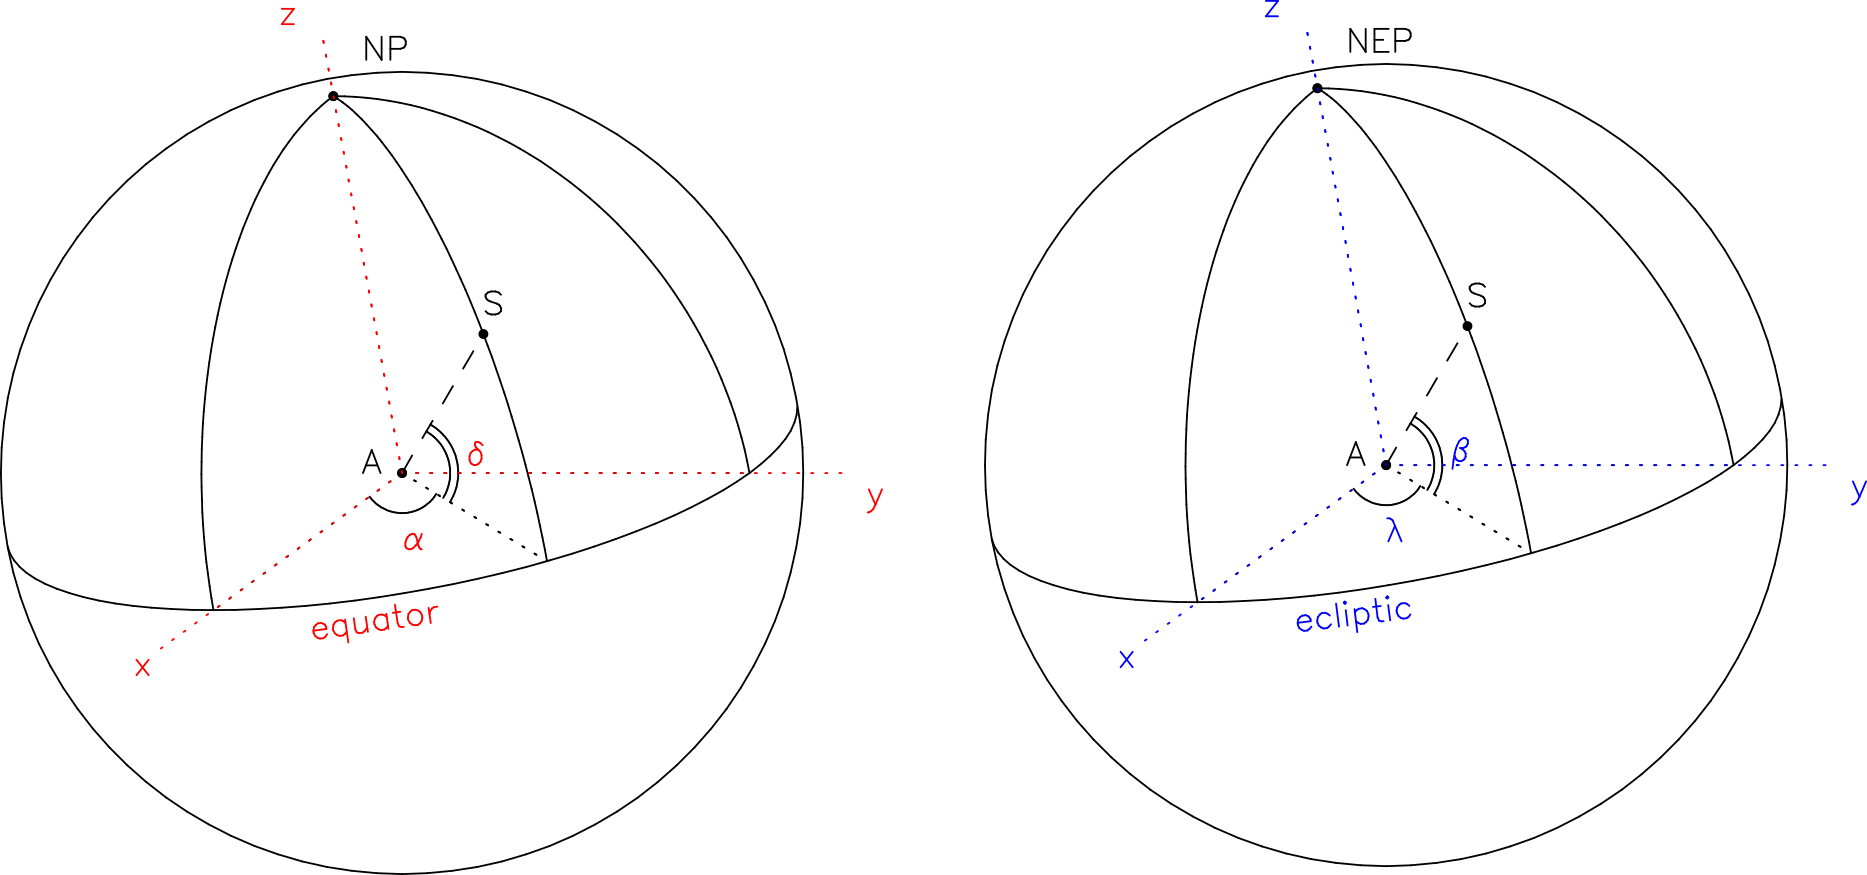
\includegraphics[width=\linewidth]{cel.png}
    \caption{Celestial Sphere for EQS and ECS}
\end{figure}
    
    Therefore, when someone says that Canopus has an RA of $06^h 24^m$, it means that it's RA coordinate is just over one quarter of the way around the sky (6h is one-quarter of 24h) from the First Point of Aries. RA is always measured eastward from the First Point of Aries.
\end{itemize}

\subsection{Projections}
A stereographic projection is used, as is the convention for printed star maps. A planisphere is this type of star chart. But you might encounter different projects or a map of Horizon Views, showing the stars above the horizon as seen from a specified observing site at a given date and time. Another famous projection style which we also use for geographical position is Mercator projections. You'll encounter basically these 3 types of map projections. Now we will discuss each type of these maps and their pro and cons. 

\subsubsection{Horizon Views}

Horizon views shows the portion of the sky that is viewed by a Telescope Field of View (FOV) or Human eye. In astronomy, the field of view is the amount of sky you can see, whether with your unaided vision, binoculars, or a telescope The FOV of a telescope varies due to usage of different telescope eyepieces whereas human eye spans approximately $120^\circ$ of arc. So FOV is an important part of these maps as they also provide us with a crucial information--the Range of the Sky! Also, A telescope will have a much smaller field of view, but it has significant advantages, such as greater magnification and light-gathering power. 
\begin{figure}[H]
    \centering
    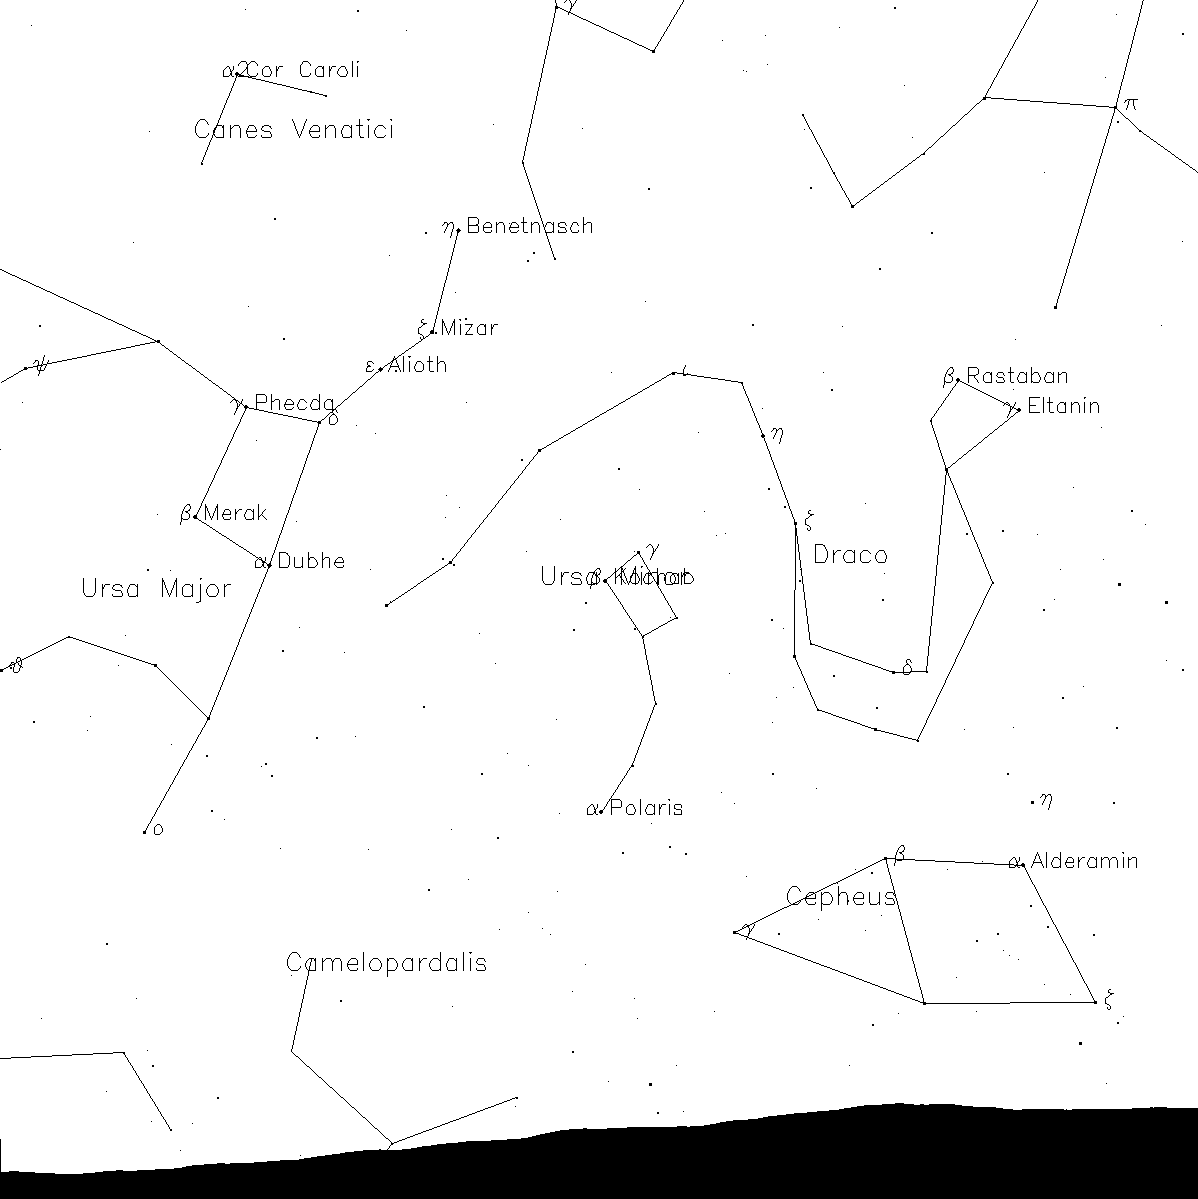
\includegraphics[width=0.6\linewidth]{Hor_1.png}
    \caption{View toward horizon from $23^\circ$ N $89^\circ$ E, azimuth $0^\circ$ (N) Wed 2022 Jan 26 0:27 UTC. Here the FOV is $75^\circ$}
\end{figure}

But to measure other information about the location of the observing place the map should contain the Pole star or the Azimuth of the sky portion should be close $0^\circ$. As we know the altitude of the Pole star is equal to the latitude of the Observing place, this makes the whole procedure easy. \\

One might ask how can we know the scale of the image? Your scale is the Ursa Major/Minor constellation itself! But with this particular viewing the longitude of the observing place can not be determined easily. But using the Dipper clock orientation you can determine the current month of the observation provided that you know the time when it was observed. This is important as same sky viewing constellation will be present at night once a year. But another thing to remember is that if you've seen this portion of the sky at midnight today, you can find the same orientation after 6 months at midday [If there was no atmosphere which we can do using Stellarium].\\

You'll get the same result for 06-26-2022 at 12:27 UTC. Don't just believe me try it yourself! A clever use of this type of maps are done in IOAA-18 O3 (See Figure \ref{A2018_O3}). 

\begin{figure}[H]
	\centering
	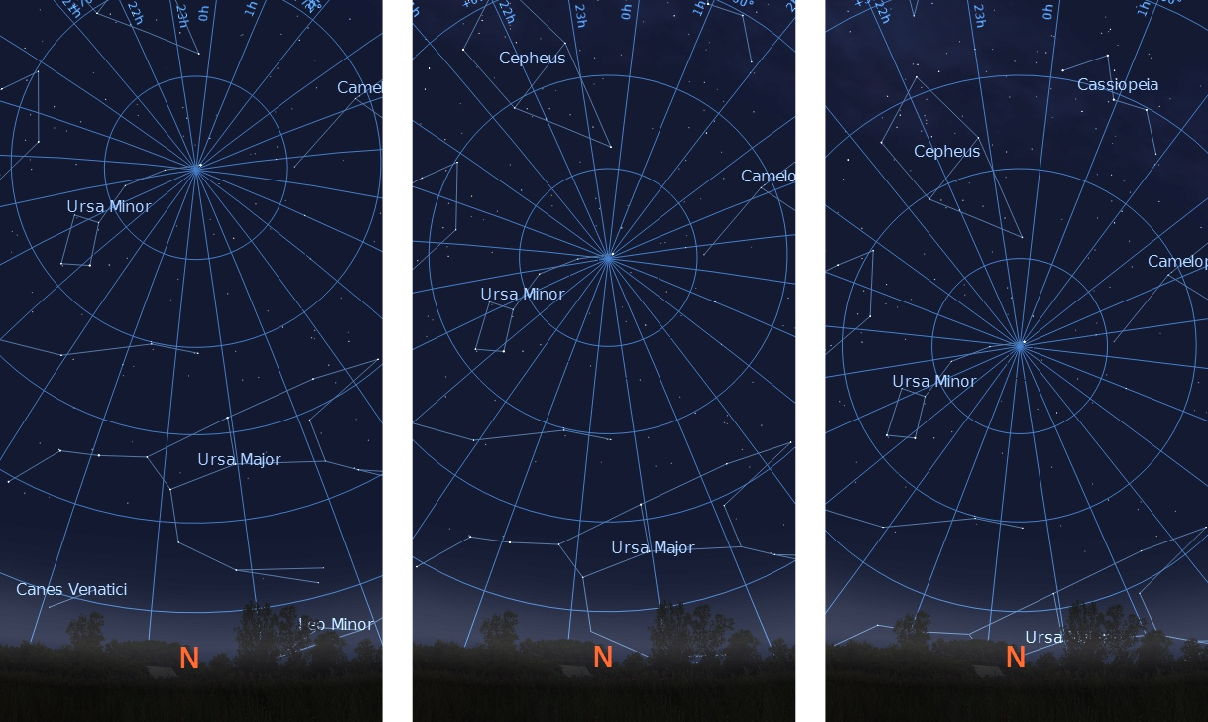
\includegraphics[width=0.9\linewidth]{skyhorizon.png}
	\caption{a) $55^\circ$ N, b) $45^\circ$ N, c) $35^\circ$ N.}
\end{figure}
The effect of changing latitude on Horizon views. Travelling south causes constellations in the north to sink towards the horizon.
\clearpage
\subsubsection{Round Maps}

The round maps of stereographic projection shows a bird eye view of the sky. It is the most common method of presenting the sky as stated before. Let's see an example--

\begin{figure}[H]
    \centering
    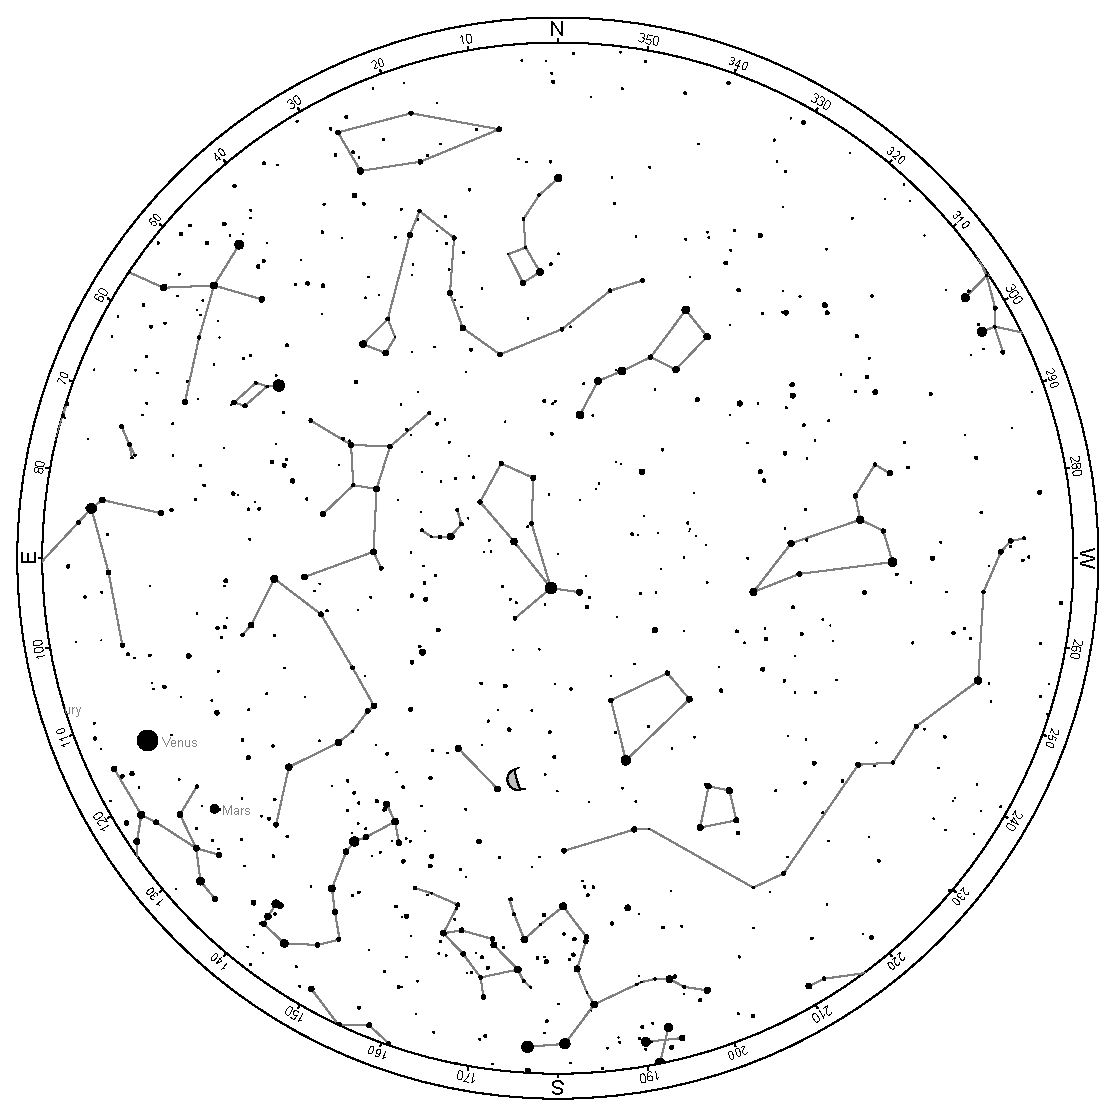
\includegraphics[width=0.9\linewidth]{stereo_1.eps}
    \caption{Stereographic projection of sky above $23.5^\circ$ North}
    \label{stereo_2}
\end{figure}

The round edge of each chart represents your horizon, with compass directions usually labeled. If not, then try to find the pole star. The line joining pole star and the center of the map reaches the both North and South cardinals. The side which is closest to Pole star is obviously your North. Turn the map around so the edge marked with the direction you’re facing (north, east, or whatever) is right-side up. The stars above this horizon on the map will now match the stars you’re facing. Ignore the rest of the map for now. The map’s center is overhead (the zenith). So a star that’s plotted halfway from the edge to the center can be found about halfway up the sky. That is, it will be halfway from horizontal to straight up. Dot sizes indicate star brightness — the larger the dot, the brighter the star. Example: Let’s try the July/August chart. Turn it so the horizon labeled “Facing West” is right-side up. About halfway from there to the center is the bright star Arcturus. Go outside around one of the dates and times listed, face west, and look halfway from horizontal to straight up. There’s Arcturus! To the right of Arcturus, in the northwest, is the Big Dipper. Turn the chart so the “Facing NW” horizon edge is right side up.When you hold the chart correctly, the Dipper’s handle stretches toward the upper left and its bowl is at lower right — just the way it looks in the northwestern sky. Nearly overhead, as you crane your neck up, is the bright star Vega. It’s part of the little constellation Lyra. You’ll notice that east is left of north on our charts, not to the right as on maps of the Earth. This is because the charts are used while looking up, not down. Note: In a stereographic projection, constellations near the edge of the sky chart are stretched and appear larger than if they were at the center of the chart\\

\textbf{Some key information to notice}
\begin{itemize}
    \item The celestial equator will always go from East to West. But this imaginary line in the sky can be an arc depending on the latitude of the observer. So you must know the constellations that resides on this path. One simple example is that celestial equator passes through the belt of Orion. So if you can first determine the cardinals, you can easily draw the equator with help of Orion.
    \item The ecliptic is the imaginary path in which the Sun moves throughout the year. The term zodiac comes from this concept. There are 13 constellations that lies in the ecliptic. But 12 are considered the famous Zodiac constellations. They are: Aries, Taurus, Gemini, Cancer, Leo, Virgo, Libra, Scorpius, Sagittarius, Capricornus, Aquarius and Pisces. The Sun also passes through Ophiuchus, a constellation that has traditionally not been part of the zodiac family. It belongs to the Hercules family. One must also remember or be able to recognize this 12 constellations with their sequence. Then you can find the ecliptic.
    \item The intersection point of the equator and the ecliptic arc/line is the equinox point. So we have 2 equinox points $180^\circ$ apart. One is known as the first point of Aries \aries \; another is termed first point of Libra \libra. But the the names are misleading nowadays[!]. Yes the points are named using the constellation they were on. But due to some special effects like processional rotation the euqinoxes have shifted a bit. So the \aries \; point now lies on Pisces and \libra \; currently resides on Virgo. It is helpful to also remember their approximate position compared to nearby constellations.
\end{itemize}

Now we'll revisit the figure \ref{stereo_2} once again. Let's try to find how many things we can understand using this simple map. We will use above techniques to find out as many things as possible [See figure \ref{stereo_3}.]

\begin{enumerate}
    \item The middle point of the map serves as the Zenith of the observer, shown by \textbf{Z} in figure \ref{stereo_3}.
    \item The first thing, I've found is Big Dipper which is an asterism a part of big and famous constellation Ursa Major.
    \item As you see it’s a map of Northern hemisphere. How can I tell? I've found Ursa Minor and it's brightest star Polaris! From basic celestial sphere knowledge we know that the altitude of Polaris is equal to Observer's Latitude.
    \item Using Polaris and \textbf{Z} point we can estimate the cardinals-- N,S,E,W. Notice that E and W are mirror than what is supposed to be. 
    \item From Big Dipper using the star Alkaid, using an arrow we can find brightest star (\nth{4} Brightest) of Bootes constellation, Arcturus! Shown using blue arrows, this is called star hopping. You can create your own star hopping shortcuts! We may discuss it later.
    \item Again, It's obviously night sky of Summer Season! How can I tell? Using another famous asterism Summer Triangle!
    \item Using the Zodiac Constellations--Cancer, Leo, Virgo, Libra, Scorpius, and part of Sagittarius, we can determine the approx. path of the Sun also known as Ecliptic. Green line in the figure \ref{stereo_3}.
    \item Scorpius constellation is also known as Fish Hook asterism.
    \item The first point of Libra \libra , where the Ecliptic intersects with the Equator is also a known location. This location was once above Libra but it has now shifted to Virgo. Shown using a circled cross in figure \ref{stereo_3}. 
\end{enumerate}

\begin{figure}[H]
    \centering
    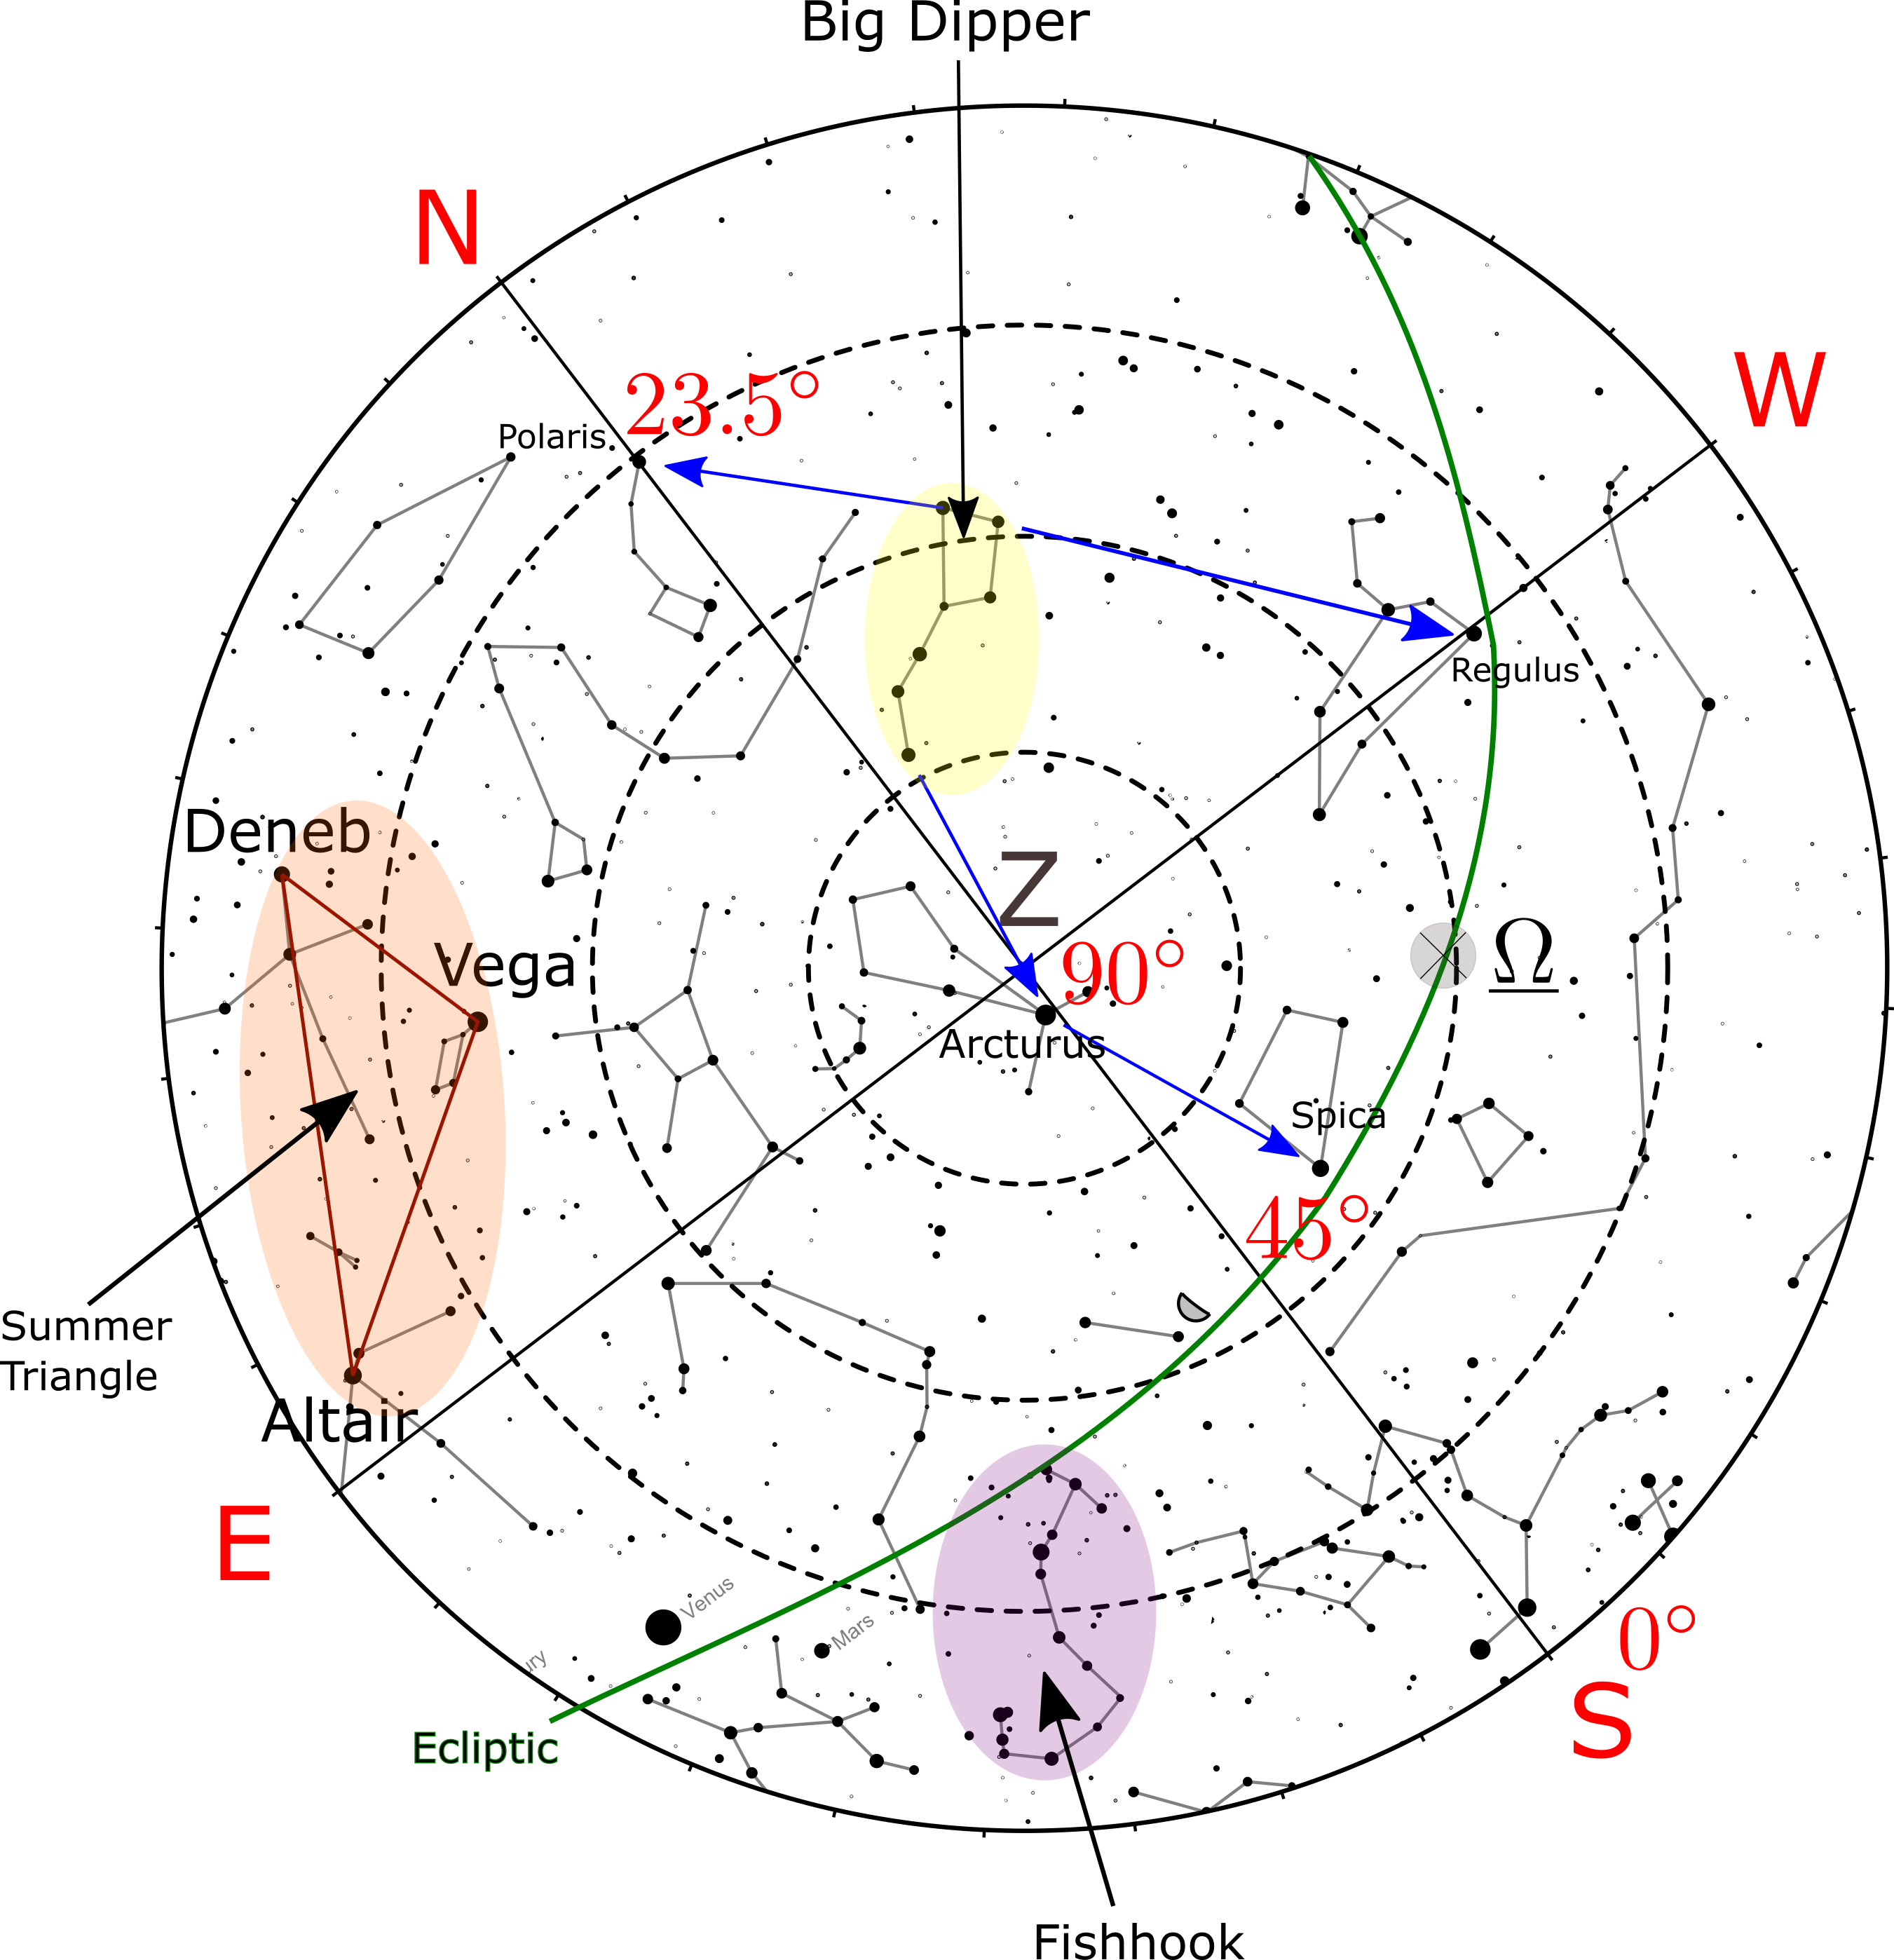
\includegraphics[width=0.9\linewidth]{solved_map1.png}
    \caption{Solved Map for figure \ref{stereo_2}.}
    \label{stereo_3}
\end{figure}
\clearpage
\subsection{Pole View Maps}
Pole view maps are interesting as here the edge of the map represents both the observing horizon in horizontal coordinate system and equator for equatorial coordinate system. So with this, one can determine the position of the star in both measuring system. \\
\begin{figure}[H]
    \centering
    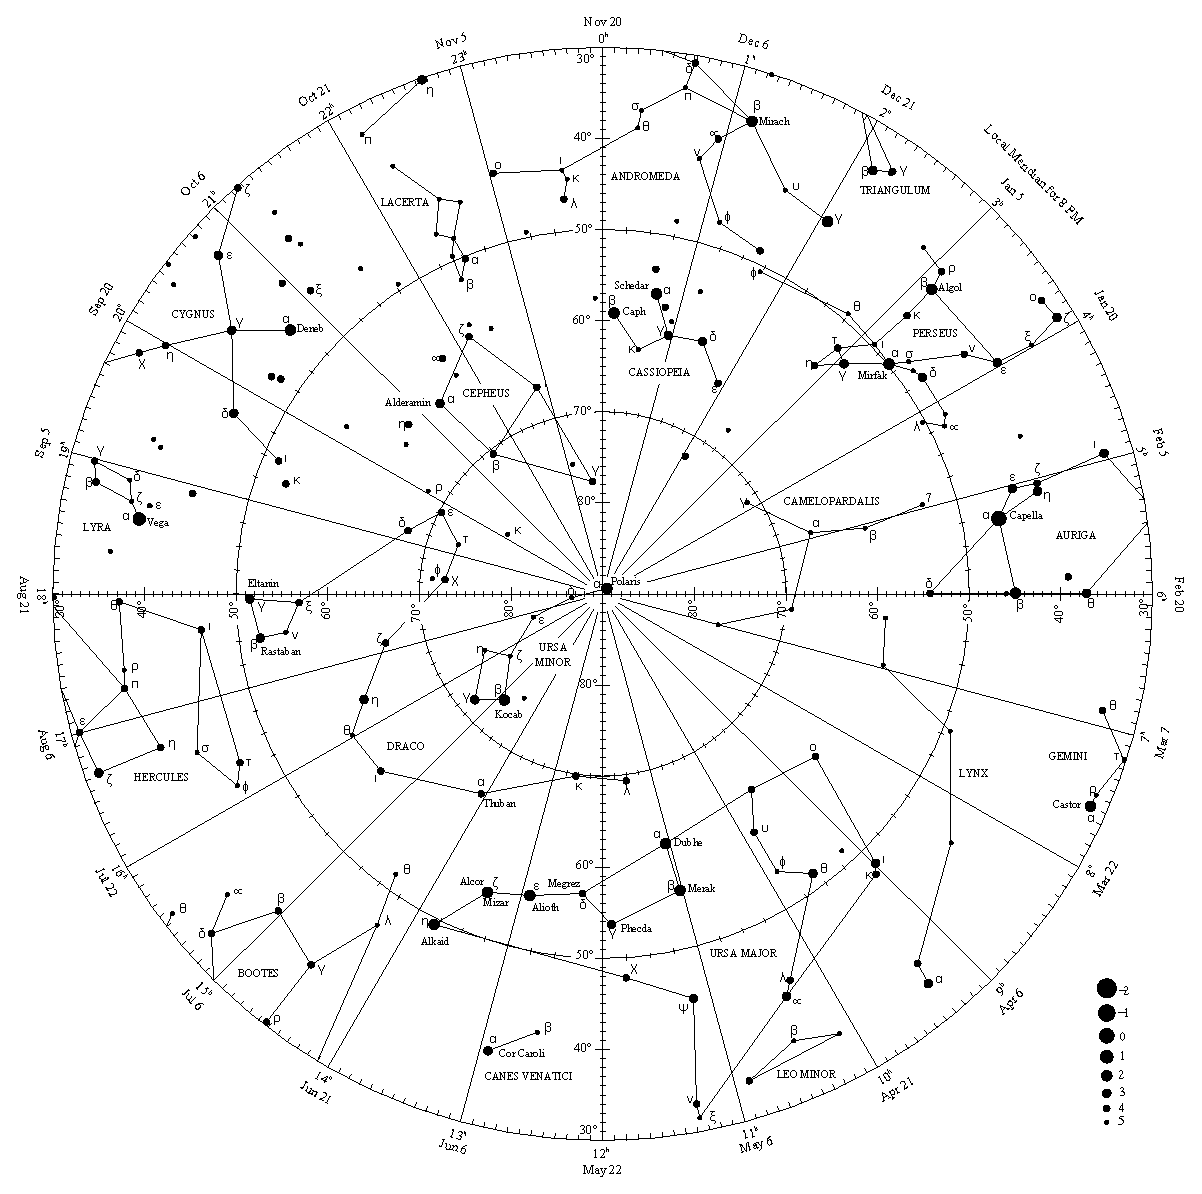
\includegraphics[width=0.9 \linewidth]{ncp_view.eps}
    \caption{View from North Celestial Pole}
\end{figure}


\begin{figure}[H]
    \centering
    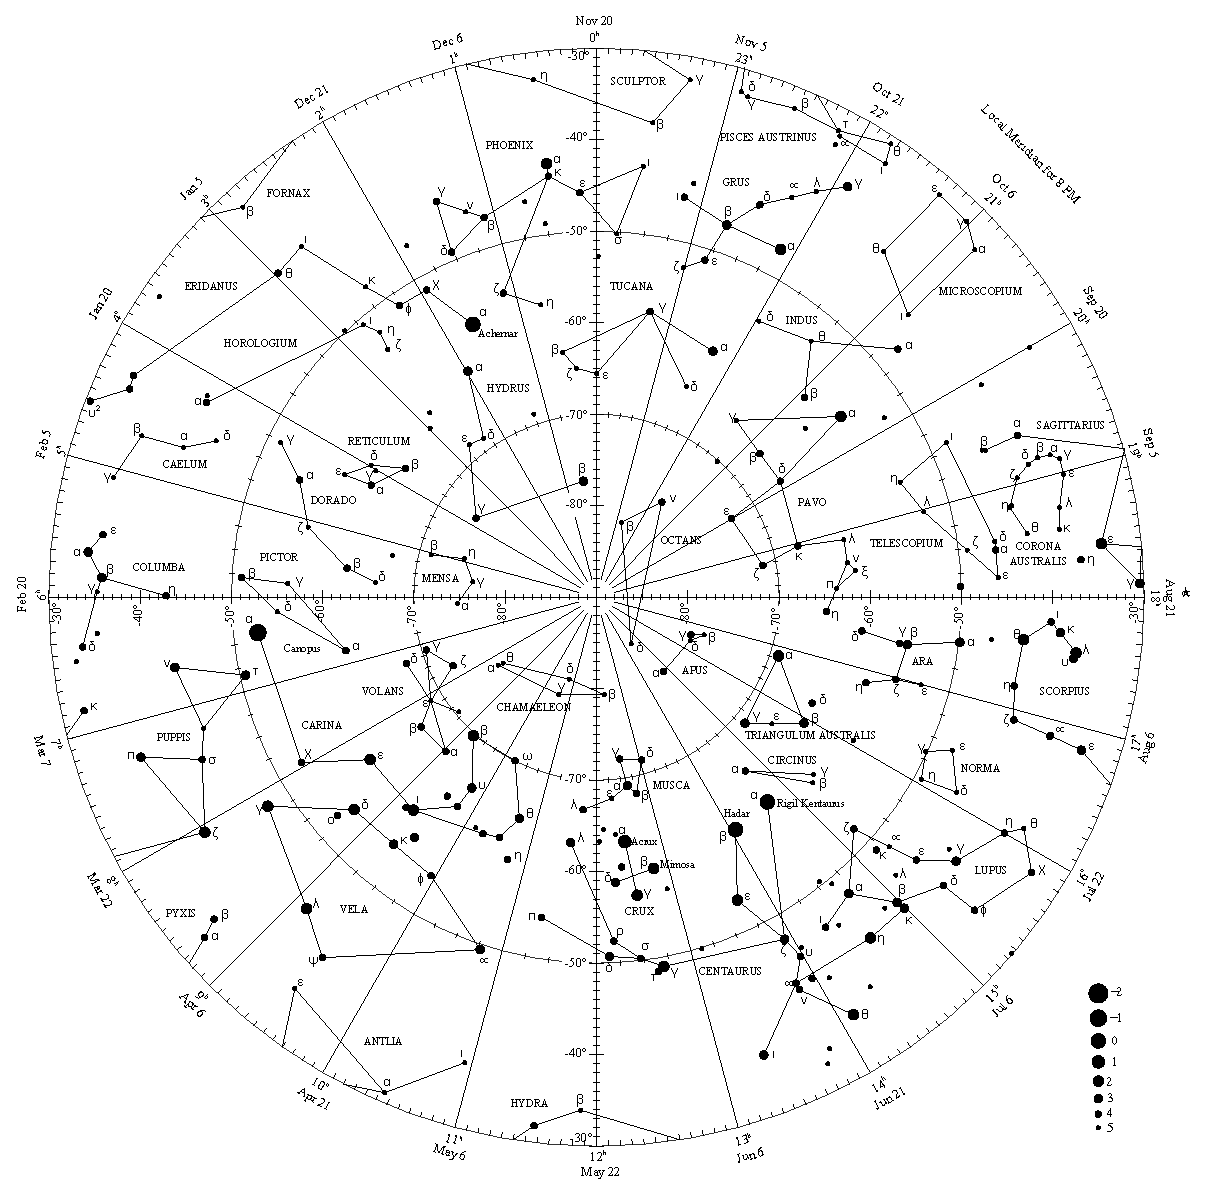
\includegraphics[width=0.9 \linewidth]{scp_view.eps}
    \caption{View from South Celestial Pole}
\end{figure}

\subsubsection{The precession of the equinoxes}

The precession of the equinoxes is a gradual changing in the direction of the Earth’s rotation axis, which causes the position of the celestial poles to drift through the constellations at a continuous rate of roughly 20 arcseconds per year. Although this effect is small on short timescales, the accumulated drift adds up to about one Moon diameter per century.\\

Currently the Earth’s north celestial pole points close to the star Polaris, but this will not always be the case. By 2500, Polaris will be several degrees away from the true celestial pole.\\

Suppose that at a certain point in time the star has coordinates ($\alpha_{old}, \delta_{old}$) and ($\lambda_{old}, \beta$). It is necessary to calculate its coordinates ($\alpha_{new}, \delta_{new}$) and ($\lambda_{new}, \beta$) after time $t$ 

$$\sin\beta=\cos\varepsilon \sin\delta_{old}-\sin\varepsilon\cos\delta_{old}\sin\alpha_{old}$$
$$\sin\lambda_{old}=\frac{\sin\delta_{old}-\cos\varepsilon \sin\beta}{\sin\varepsilon \cos\beta}$$

$$\cos\lambda_{old}=\frac{\cos\delta_{old}\cos\alpha_{old}}{\cos\beta}$$
Again, 

$$\lambda_{new}=\lambda_{old}+\frac{t}{26000\; years}\ast 360^\circ$$

$$\delta_{new}=\arcsin(\cos\varepsilon\sin\beta+\sin\varepsilon\cos\beta \sin\lambda_{new})$$
$$\sin\alpha_{new}=\frac{\cos\varepsilon\sin\lambda_{new}-\sin\beta}{\sin\varepsilon\cos\delta_{new}}$$
$$\cos\alpha_{new}=\frac{\cos\beta\cos\lambda_{new}}{\cos\delta_{new}}$$

\begin{figure}[H]
	\centering
	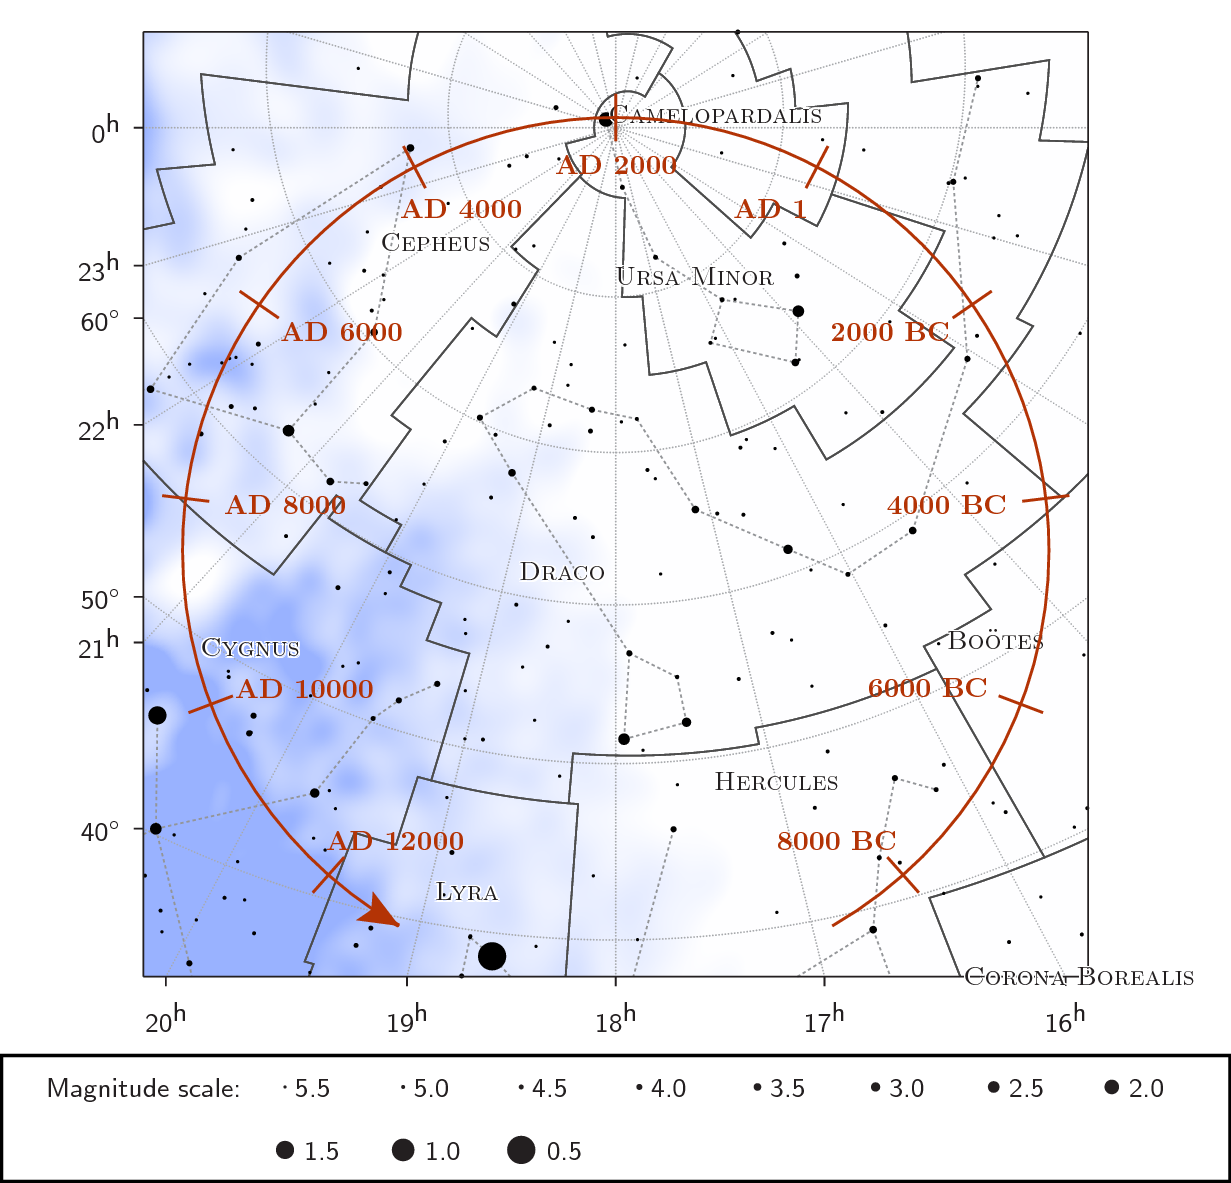
\includegraphics[width=0.7 \linewidth]{presc1.png}
	\caption{Precessional Circle}
	\label{pcircle}
\end{figure}
Right now, Polaris ($\alpha$ Ursa Minor) is the ``north pole star'', however Thuban ($\alpha$ Draco) was the ``north pole star'' when it was around 3000 BC.

\begin{enumerate}[Q1.]
	\item Mark Thuban on Figure \ref{precession}
	\item We know that Thuban was passed by north celestial pole, and Polaris is also passed by north celestial pole. Based on this, we can find the north ecliptic pole. Find the north ecliptic pole!
	\item Measure the period of the precession.
	\item Find the equatorial coordinate of Polaris when Thuban was the ``north pole star''.
\end{enumerate}

\textbf{Answers}\\
\textbf{Q2} We can find the north ecliptic pole by drawing two circles with its radius of $23.5^\circ$ which the center of each circle is on Polaris and Thuban. We will get 2 intersections, E and the other one.\\
By considering the ecliptic line, we know that \textbf{E} is the north ecliptic pole (white circle), not the other one.\\

\textbf{Q3} First, we measure the angle of $\angle PET$ .There are some ways to measure this angle. Some possible methods are:
\begin{itemize}
	\item Measure PT $\rightarrow$ PT = $25.8^\circ$.
	Using cosine rule we get $\rightarrow \cos\angle PET =0.361$ or $\angle PET= 68.8^\circ$.\\
	(for cosine rule in spherical geometry, $\angle PET= 68^\circ$)
	\item Direct method (using protactor) $\angle PET= 69^\circ\; or \; 70^\circ$ (need to be measured again)
	\item Get a line from T and tangential to line PE. The intersect is at F, then : $\sin\angle PET = TF/TE$. From this method we get $\angle PET$ around $66^\circ$. (not really recommended)
\end{itemize}

Based from all these method, the range of $\angle PET= 65 -70^\circ$.
The time required to make this angle is = 3000 +20XX= 50XX years (XX = current year after 2000 CE). Thus the range of period of precession is: 25800-7800 years (These are only for the range, each team can get full mark if their answer is within this range)\\

\textbf{Q4}  $PT=25.8^\circ$, hence $\delta_{\rm polaris} = 90-PT =64.2^\circ$.\\

From sin rule, we get $\angle ETP = 58.1^\circ$ or 3h52m30s. (for sin rule in spherical geometry, it is $58.2^\circ$, still similar to flat one). We know $\alpha_{\text{North Ecliptic Pole}}=18^h$. Now, 
\begin{align*}
	\alpha_{\rm polaris}=& \alpha_{\text{North Ecliptic Pole}}+ \angle ETP\\
	\alpha_{\rm polaris}=& 21^h52^m30^s
\end{align*}

Hence, the equatorial coordinate Polaris 6000 years ago is: $(\alpha, \delta)= (21^h 52^m 30^s,\, 64.2^\circ)$

\begin{figure}[H]
	\centering
	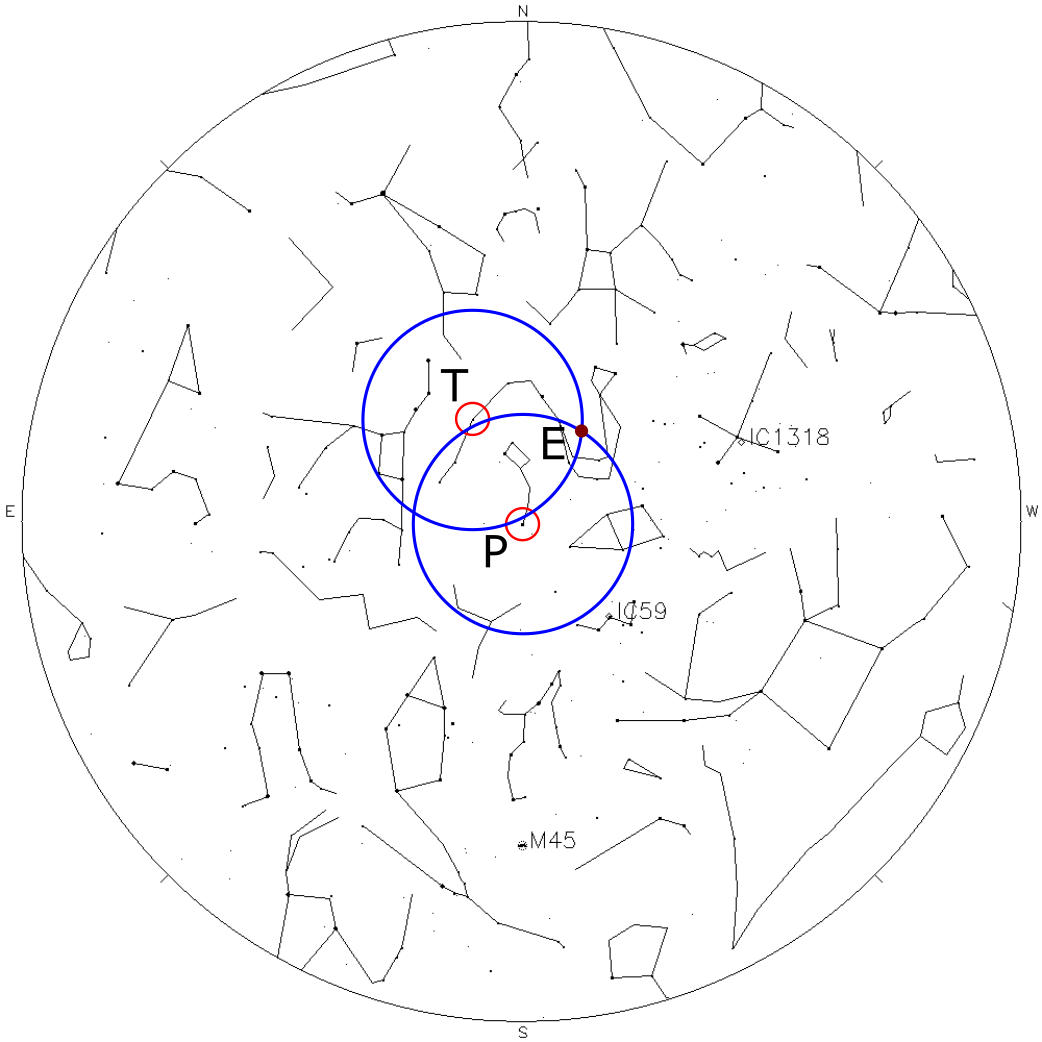
\includegraphics[width=0.8\linewidth]{thuban.png}
	\caption{Thuban as North Pole}
	\label{precession}
\end{figure}
\clearpage 
\subsubsection{Mercator Projections}
Astronomical symbols are abstract pictorial symbols used to represent astronomical objects, theoretical constructs and observational events in European astronomy. The earliest forms of these symbols appear in Greek papyrus texts of late antiquity.
\begin{figure}[H]
	\centering
	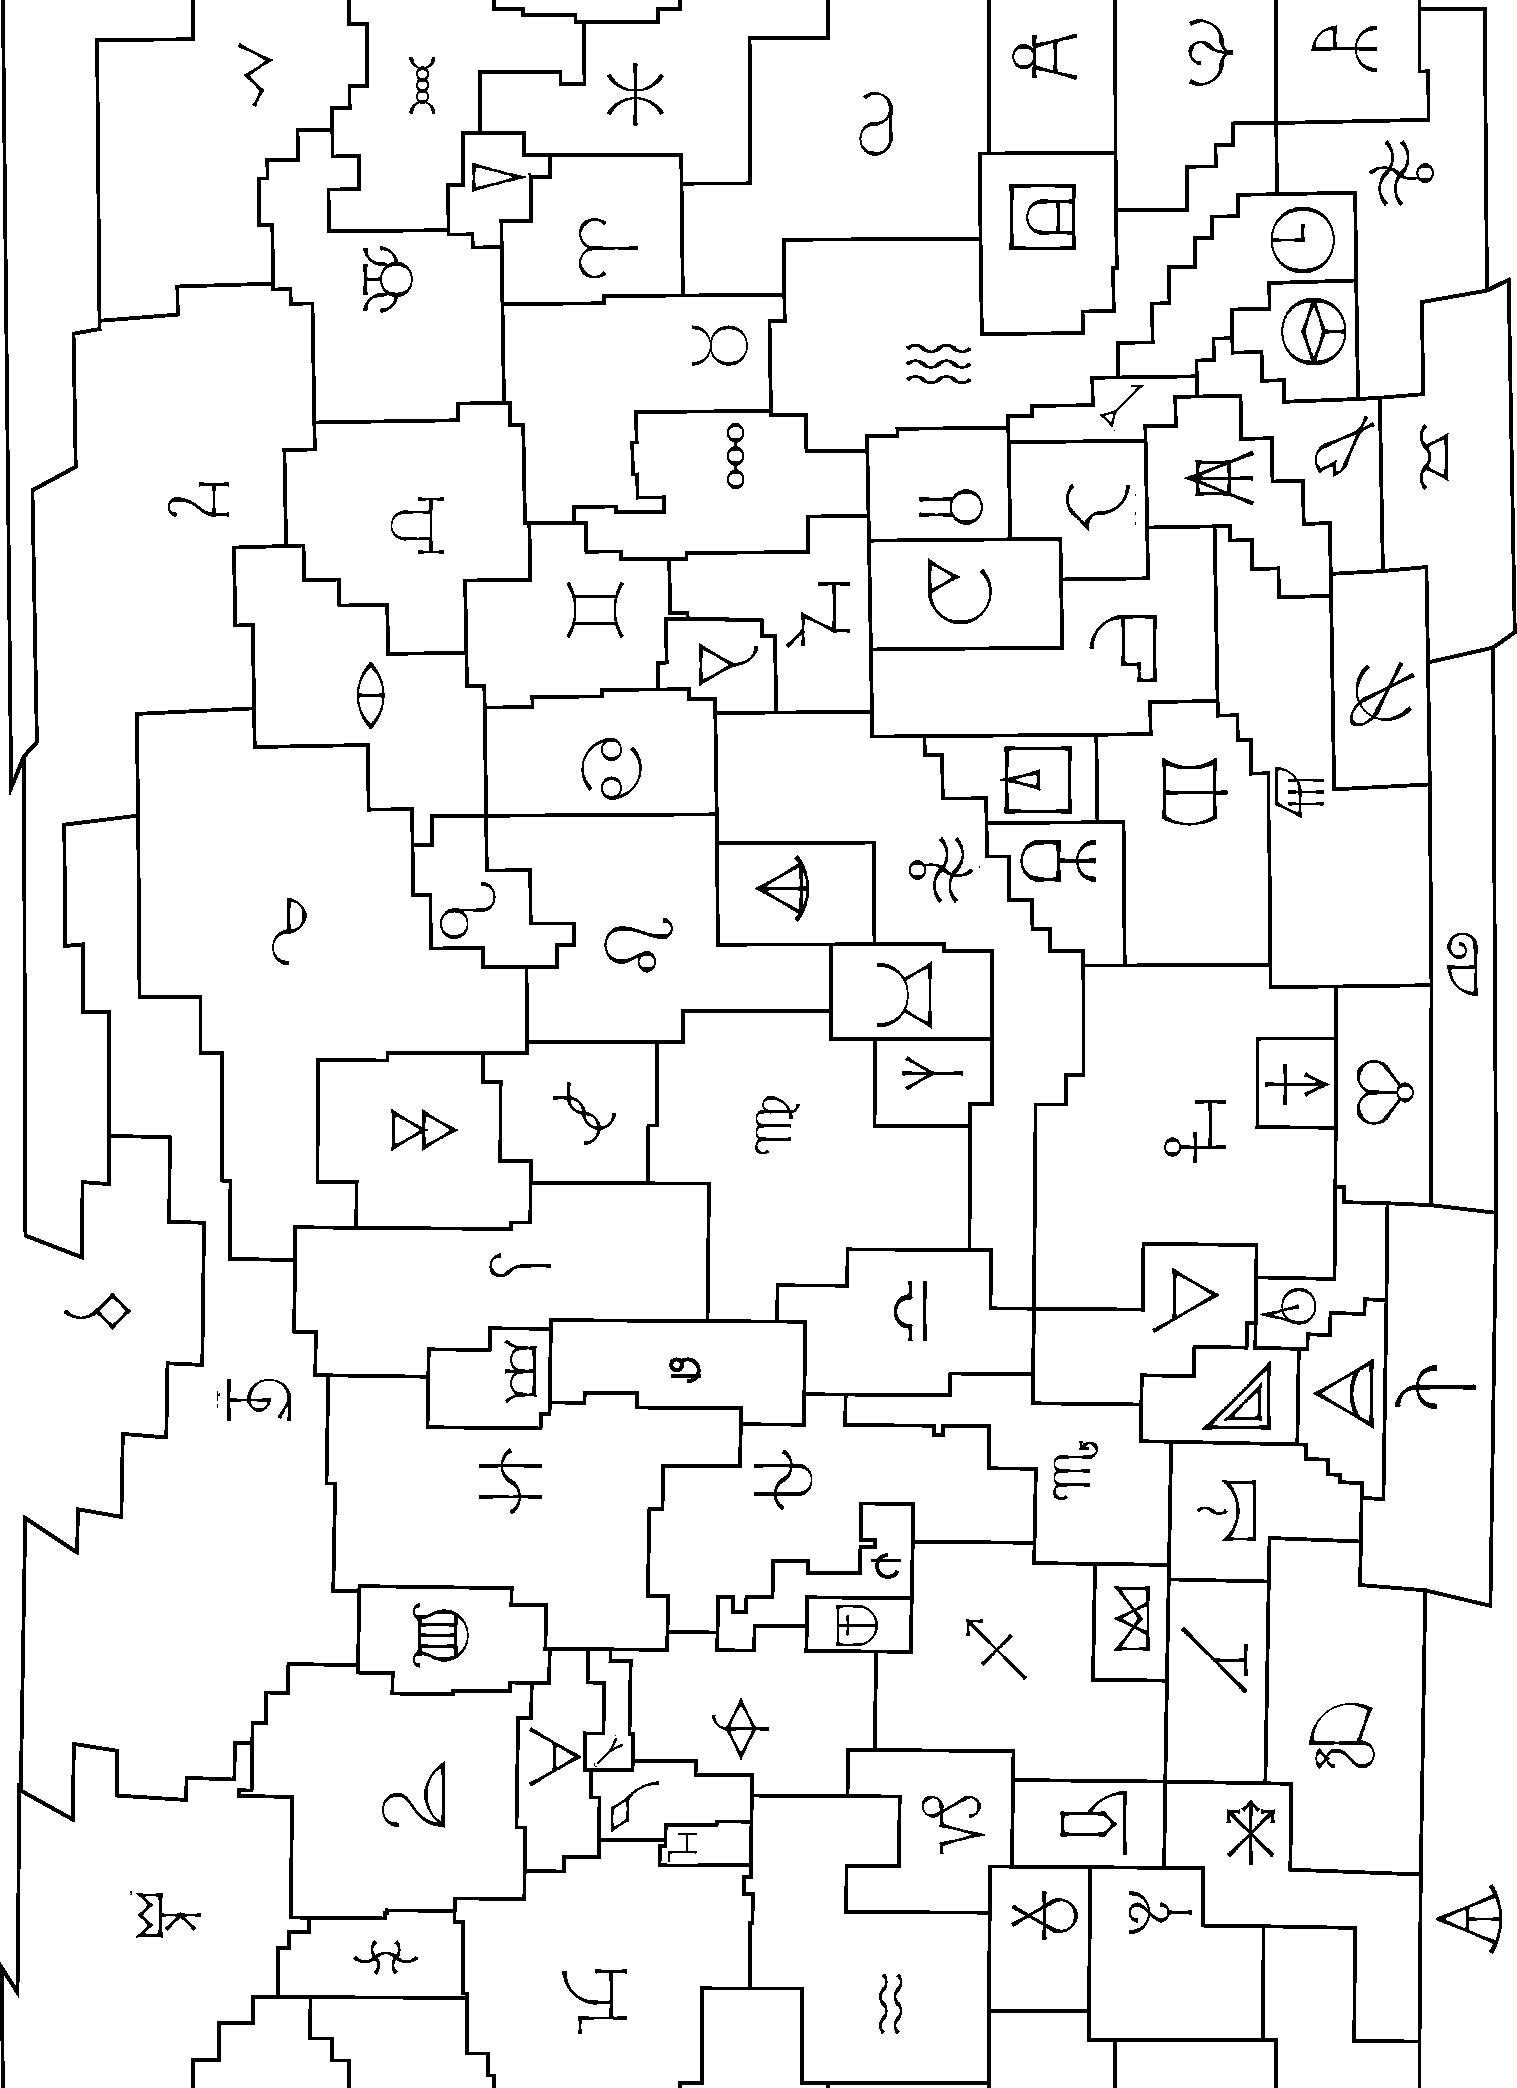
\includegraphics[width=0.8\linewidth]{starmap-glyph.png}
	\caption{Mercator-projection sky map of constellations marked with symbols}
\end{figure}

\subsection{Monthly Sky Chats}

\begin{figure}[H]
    \centering
    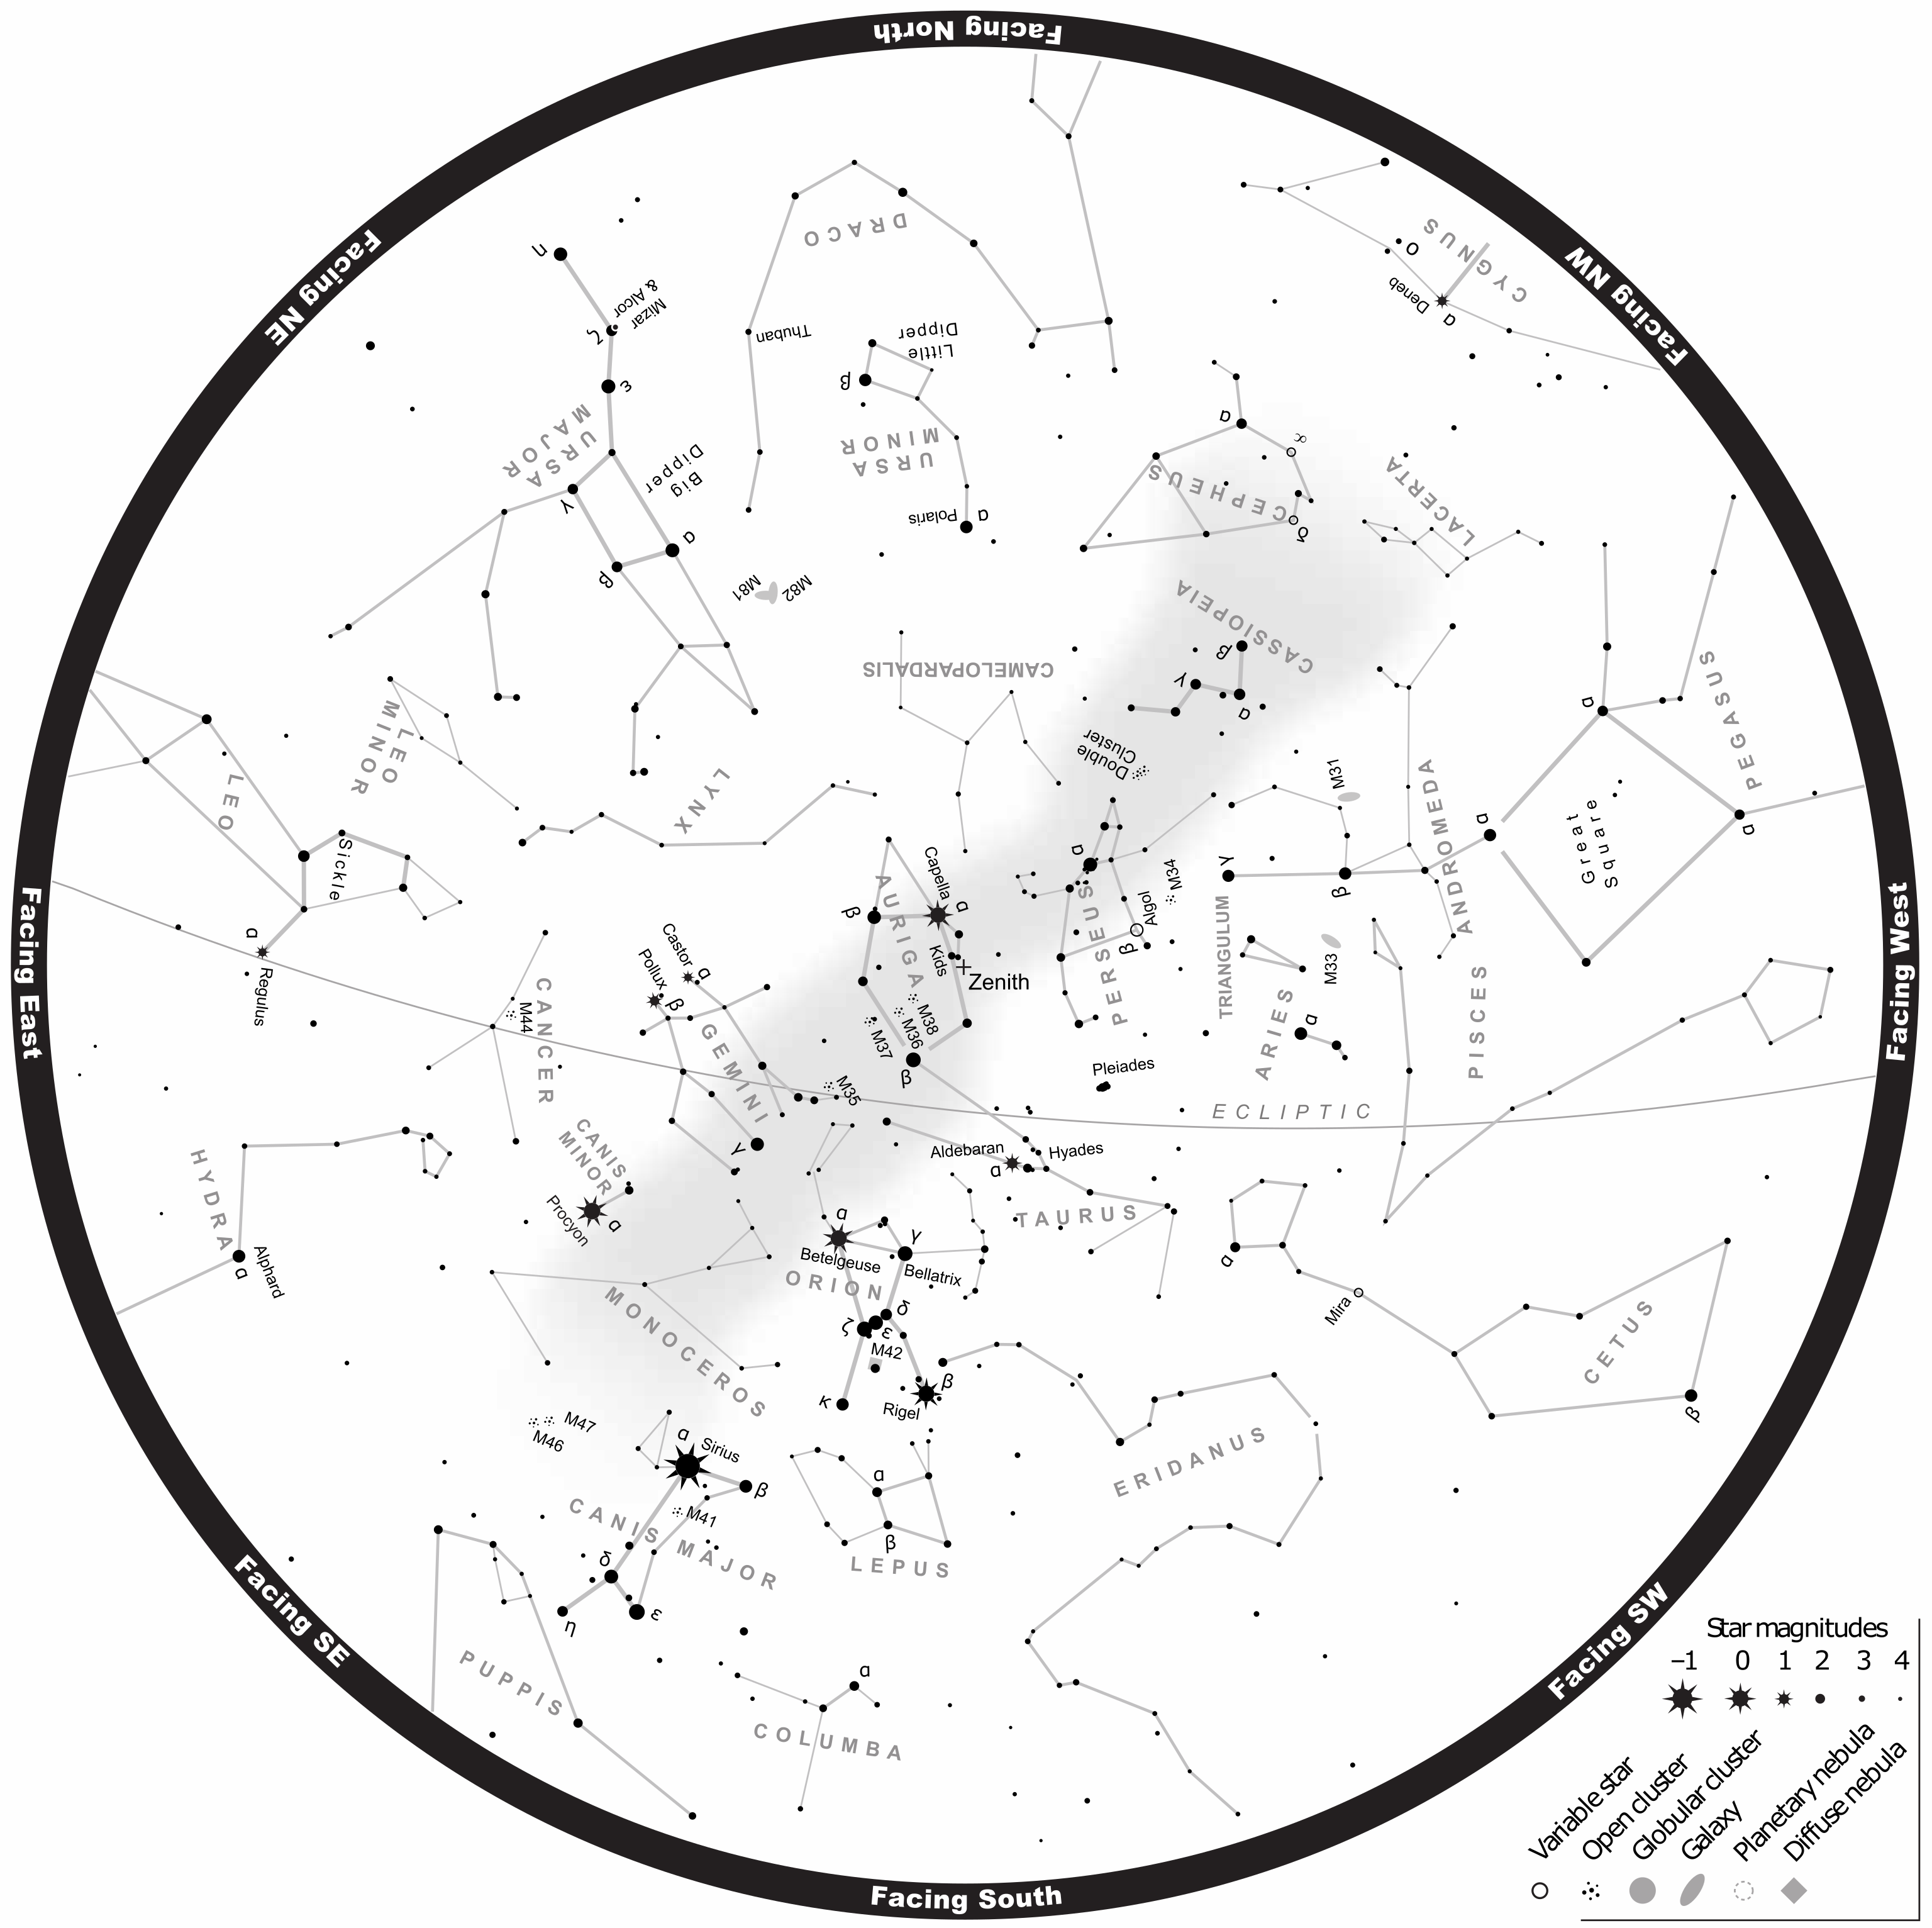
\includegraphics[width=0.9 \linewidth]{jan-feb.png}
    \caption{Jan/Feb Night Sky View for latitude $40^\circ$ N}
\end{figure}
\clearpage
\begin{figure}
    \centering
    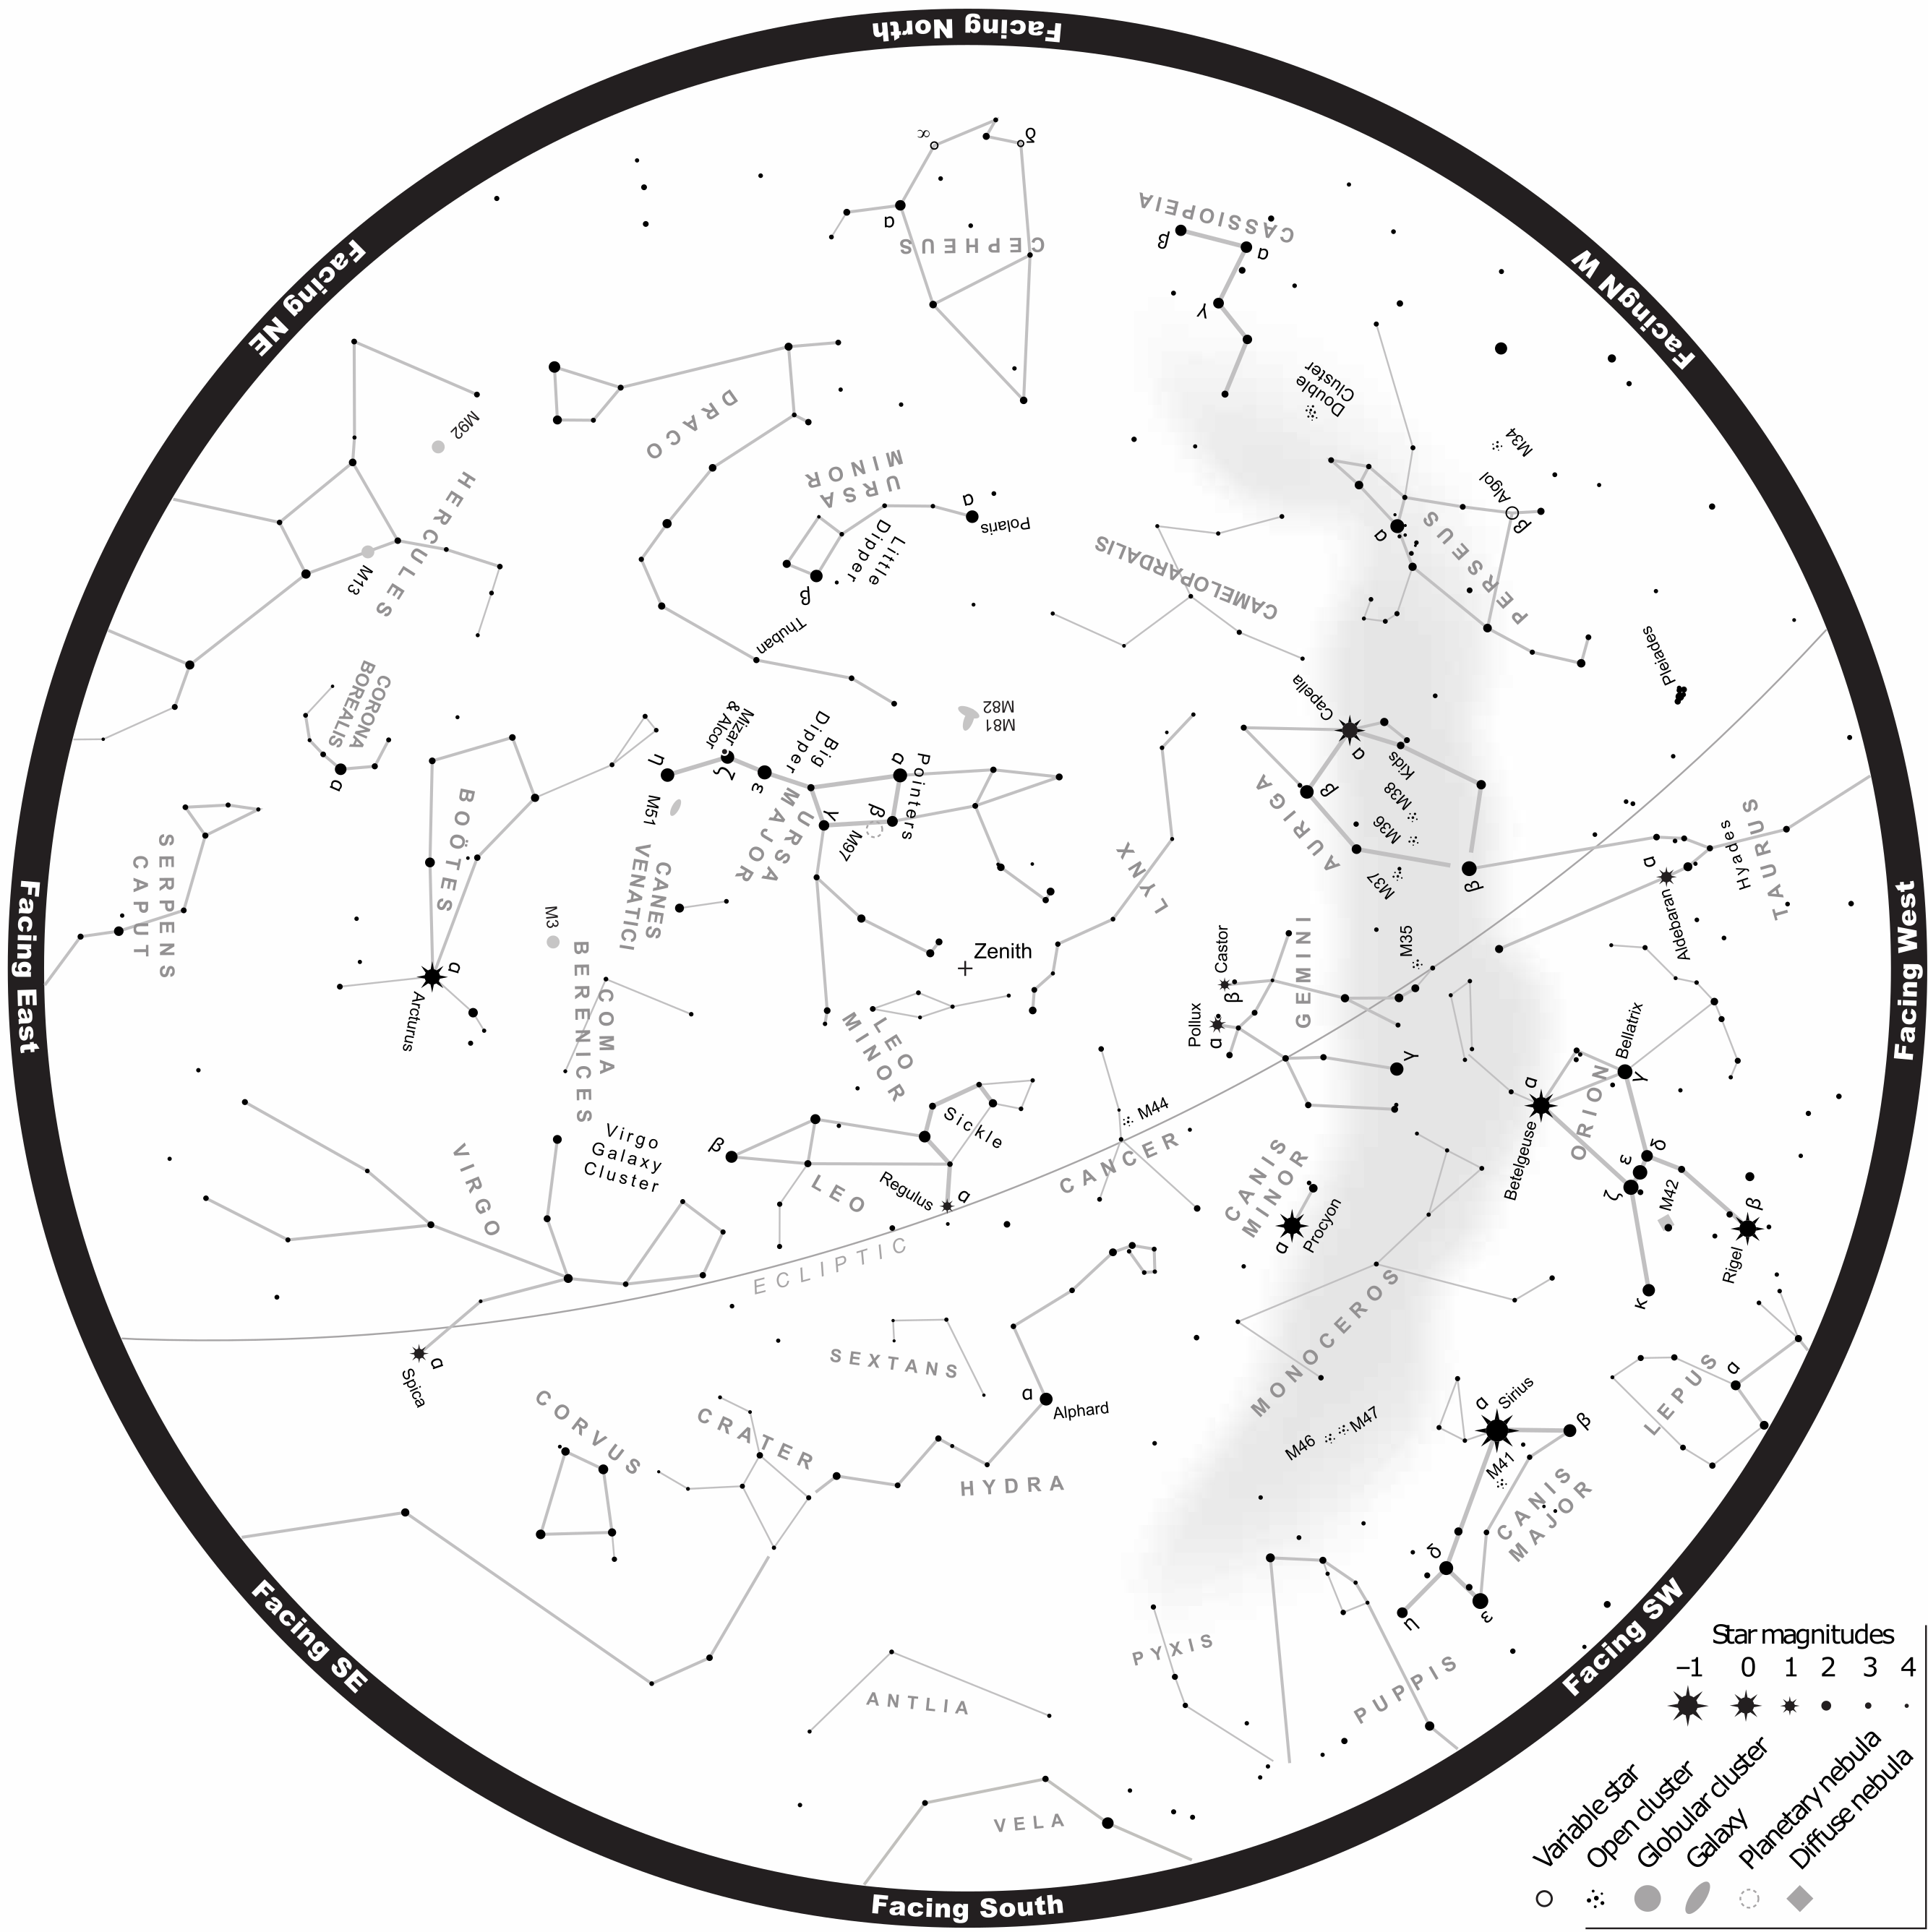
\includegraphics[width=0.9 \linewidth]{mar-apr.png}
    \caption{Mar/Apr Night Sky View for latitude $40^\circ$ N}
\end{figure}
\clearpage
\begin{figure}
    \centering
    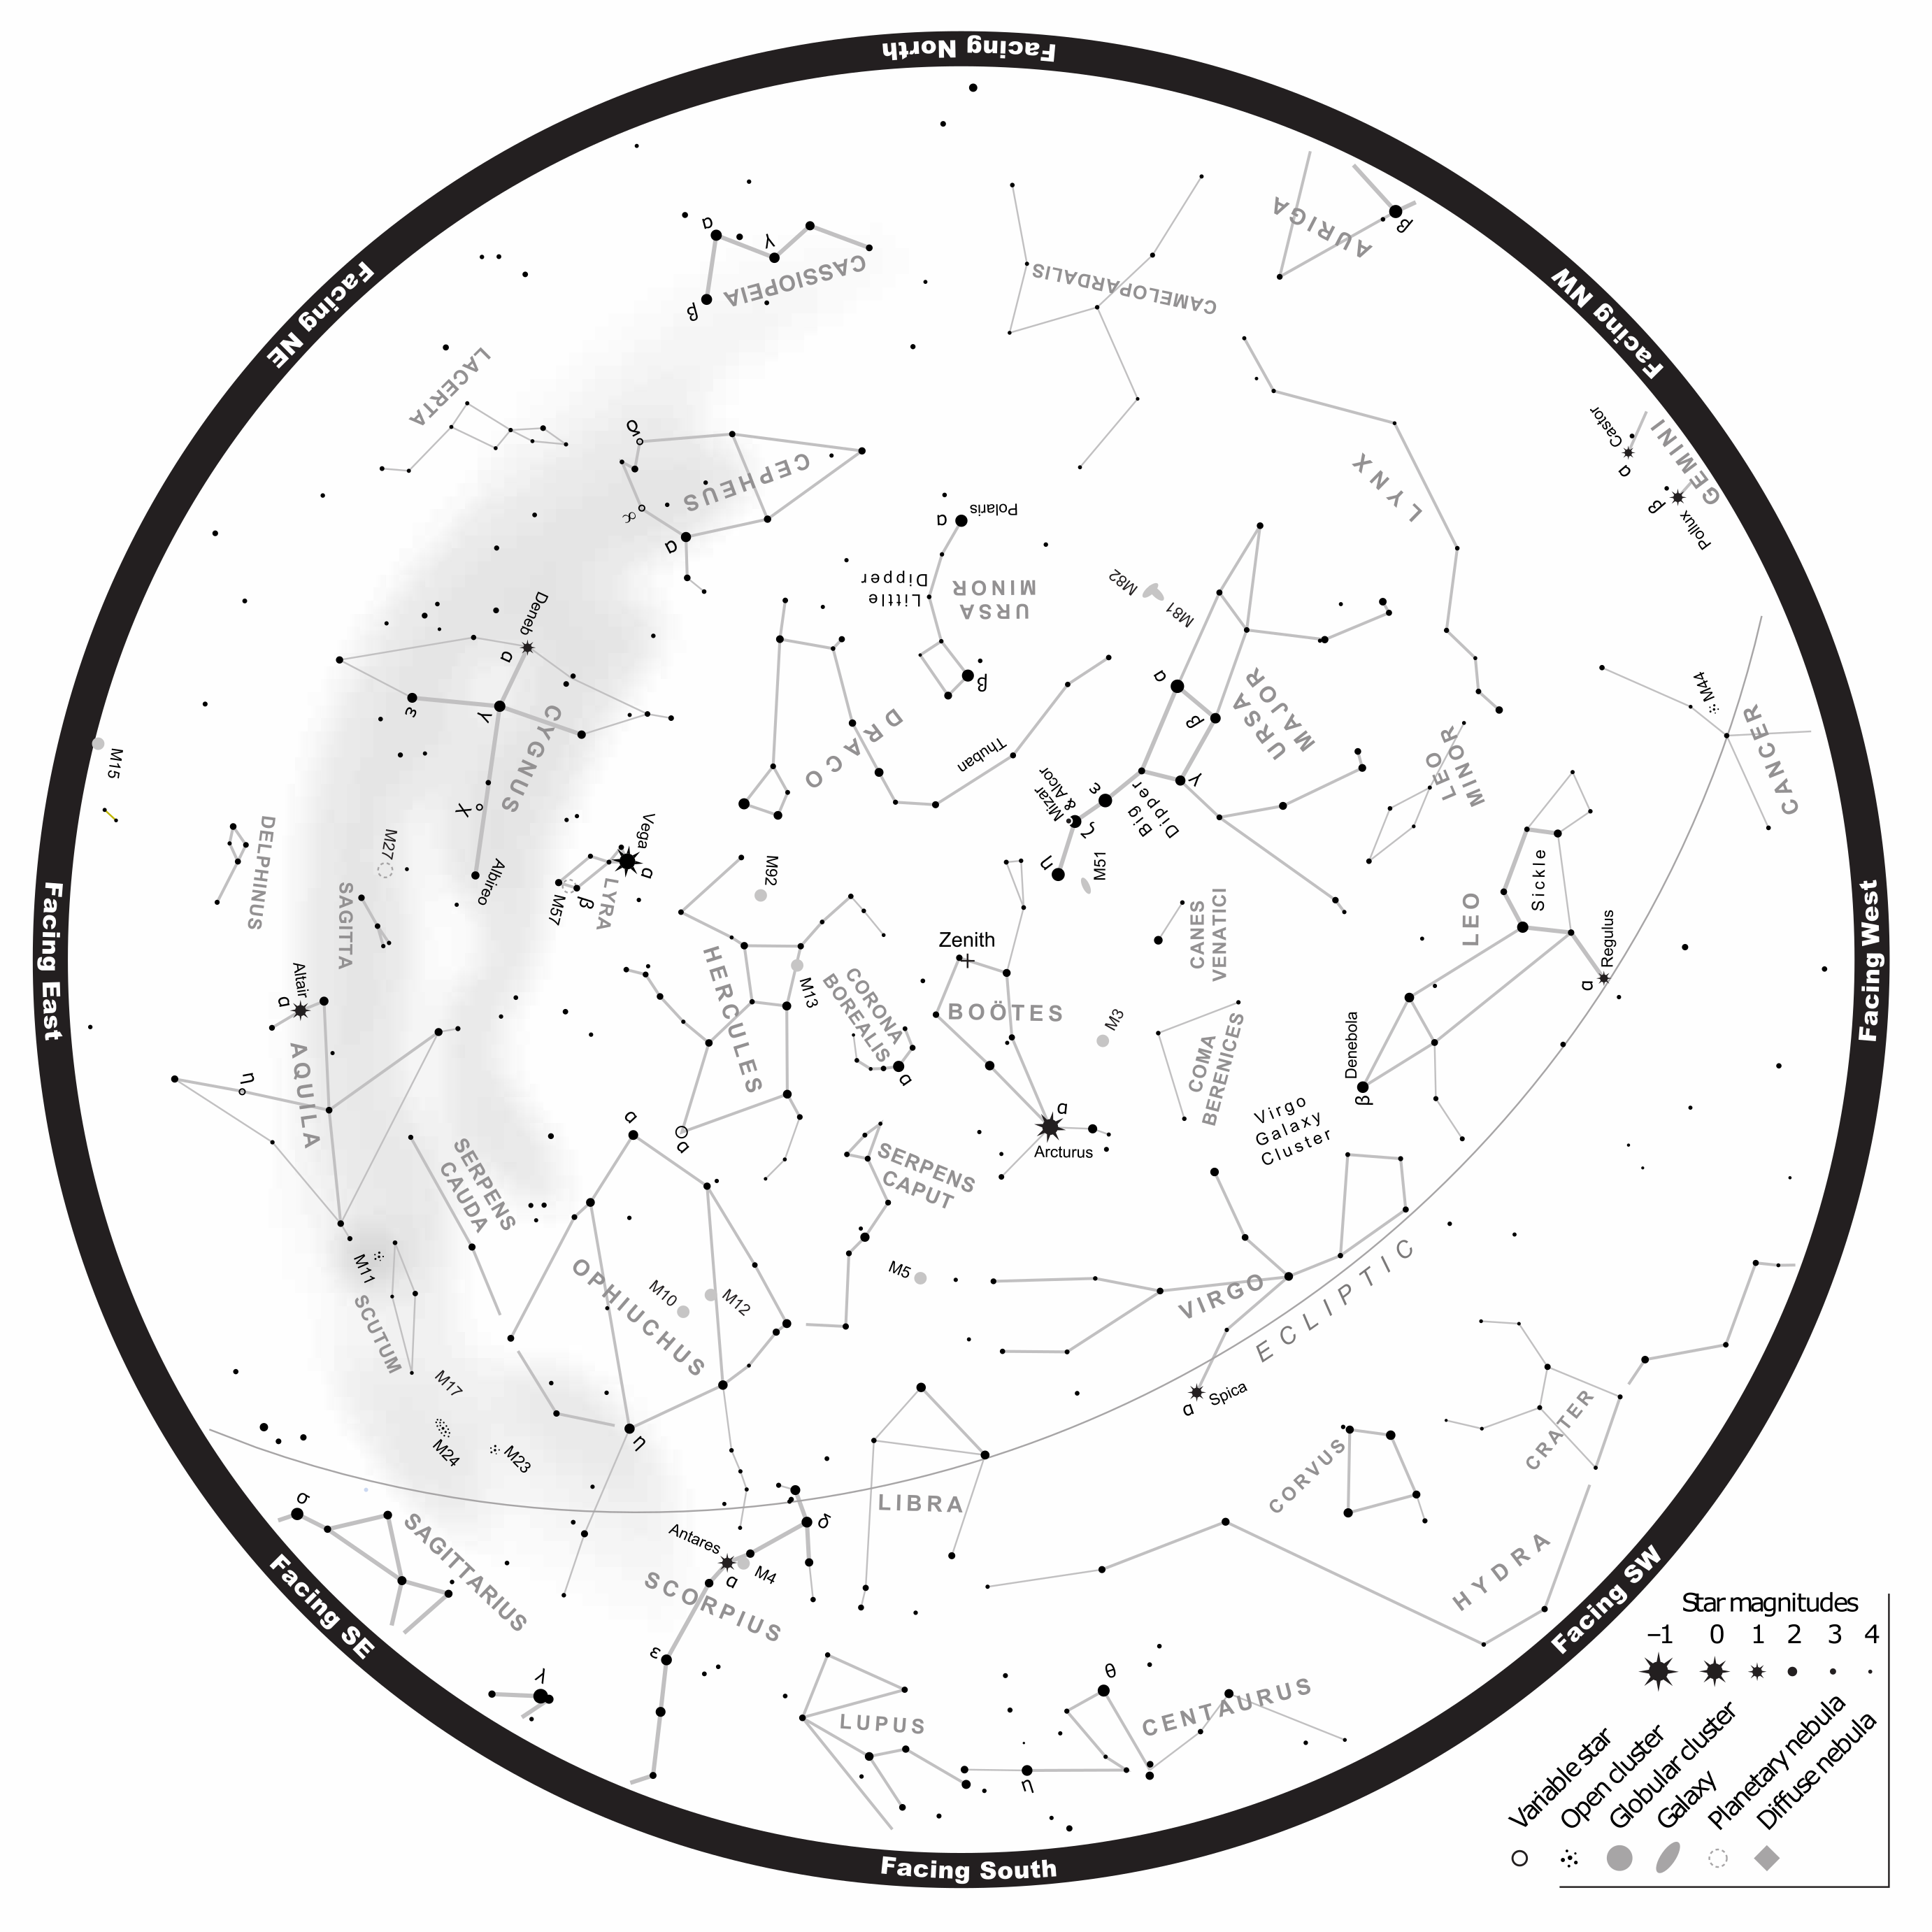
\includegraphics[width=0.9 \linewidth]{may-jun.png}
    \caption{May/Jun Night Sky View for latitude $40^\circ$ N}
\end{figure}
\clearpage
\begin{figure}
    \centering
    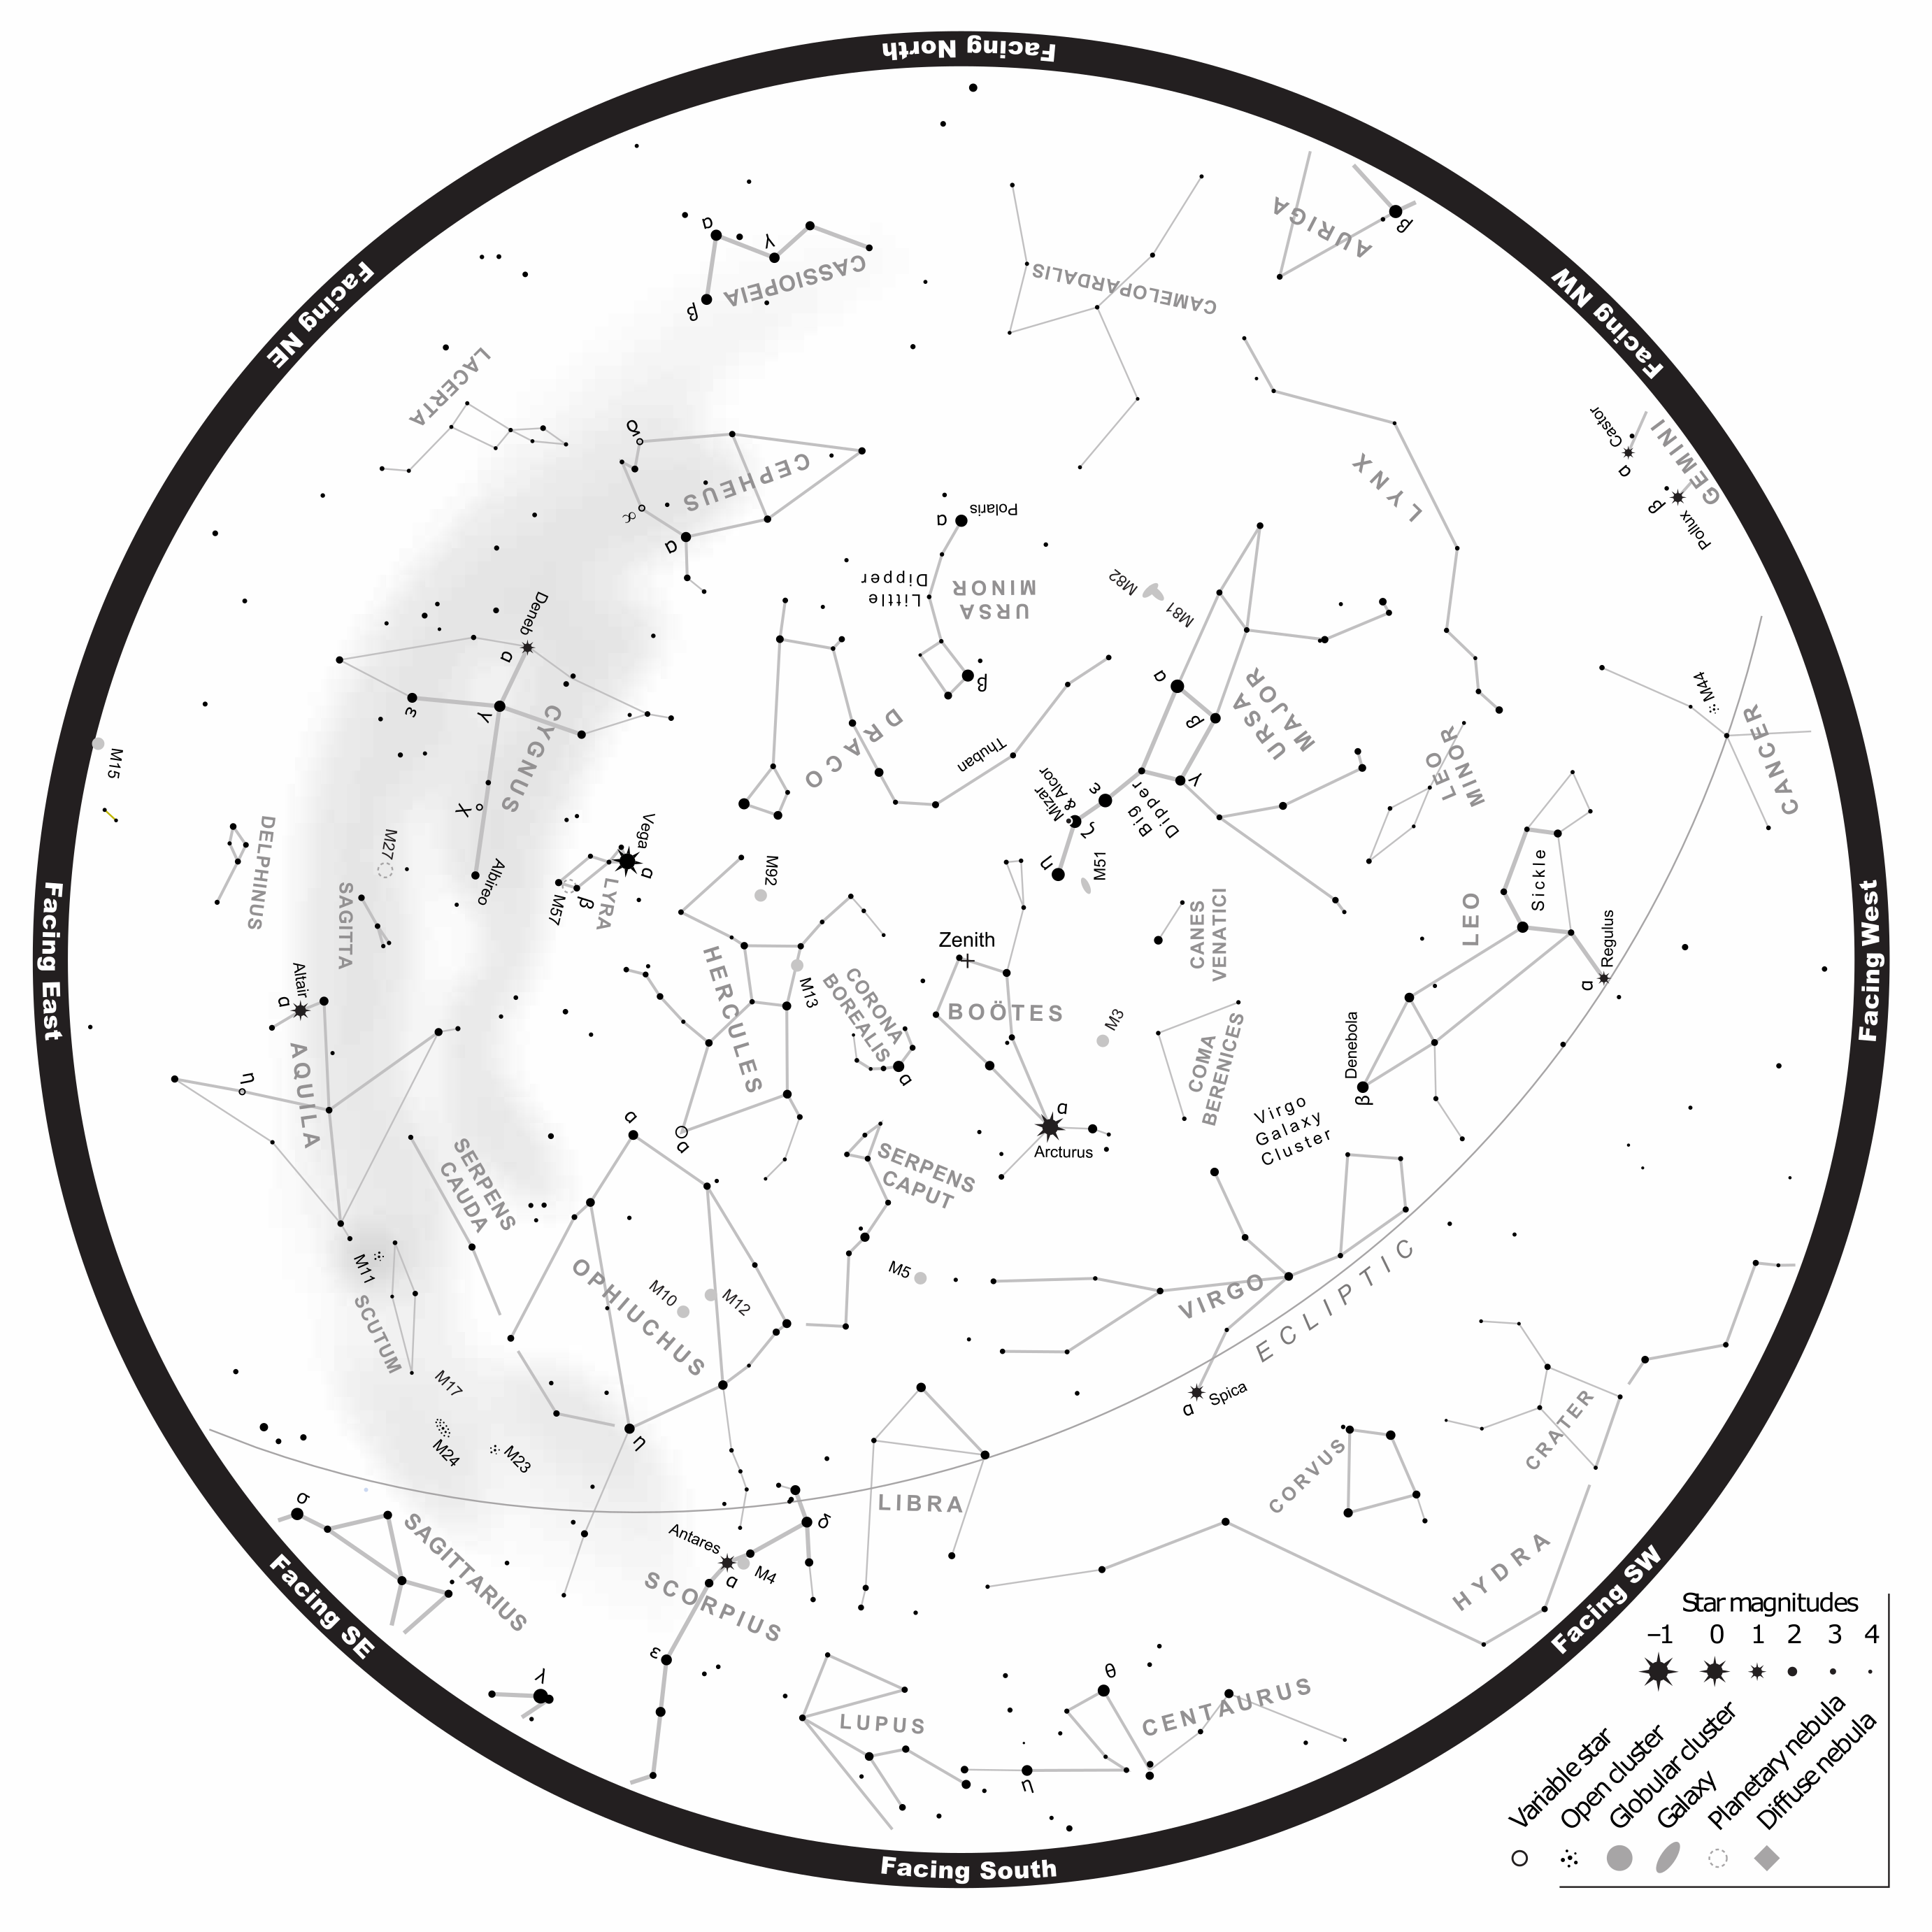
\includegraphics[width=0.9 \linewidth]{may-jun.png}
    \caption{Jul/Aug Night Sky View for latitude $40^\circ$ N}
\end{figure}
\clearpage
\begin{figure}
    \centering
    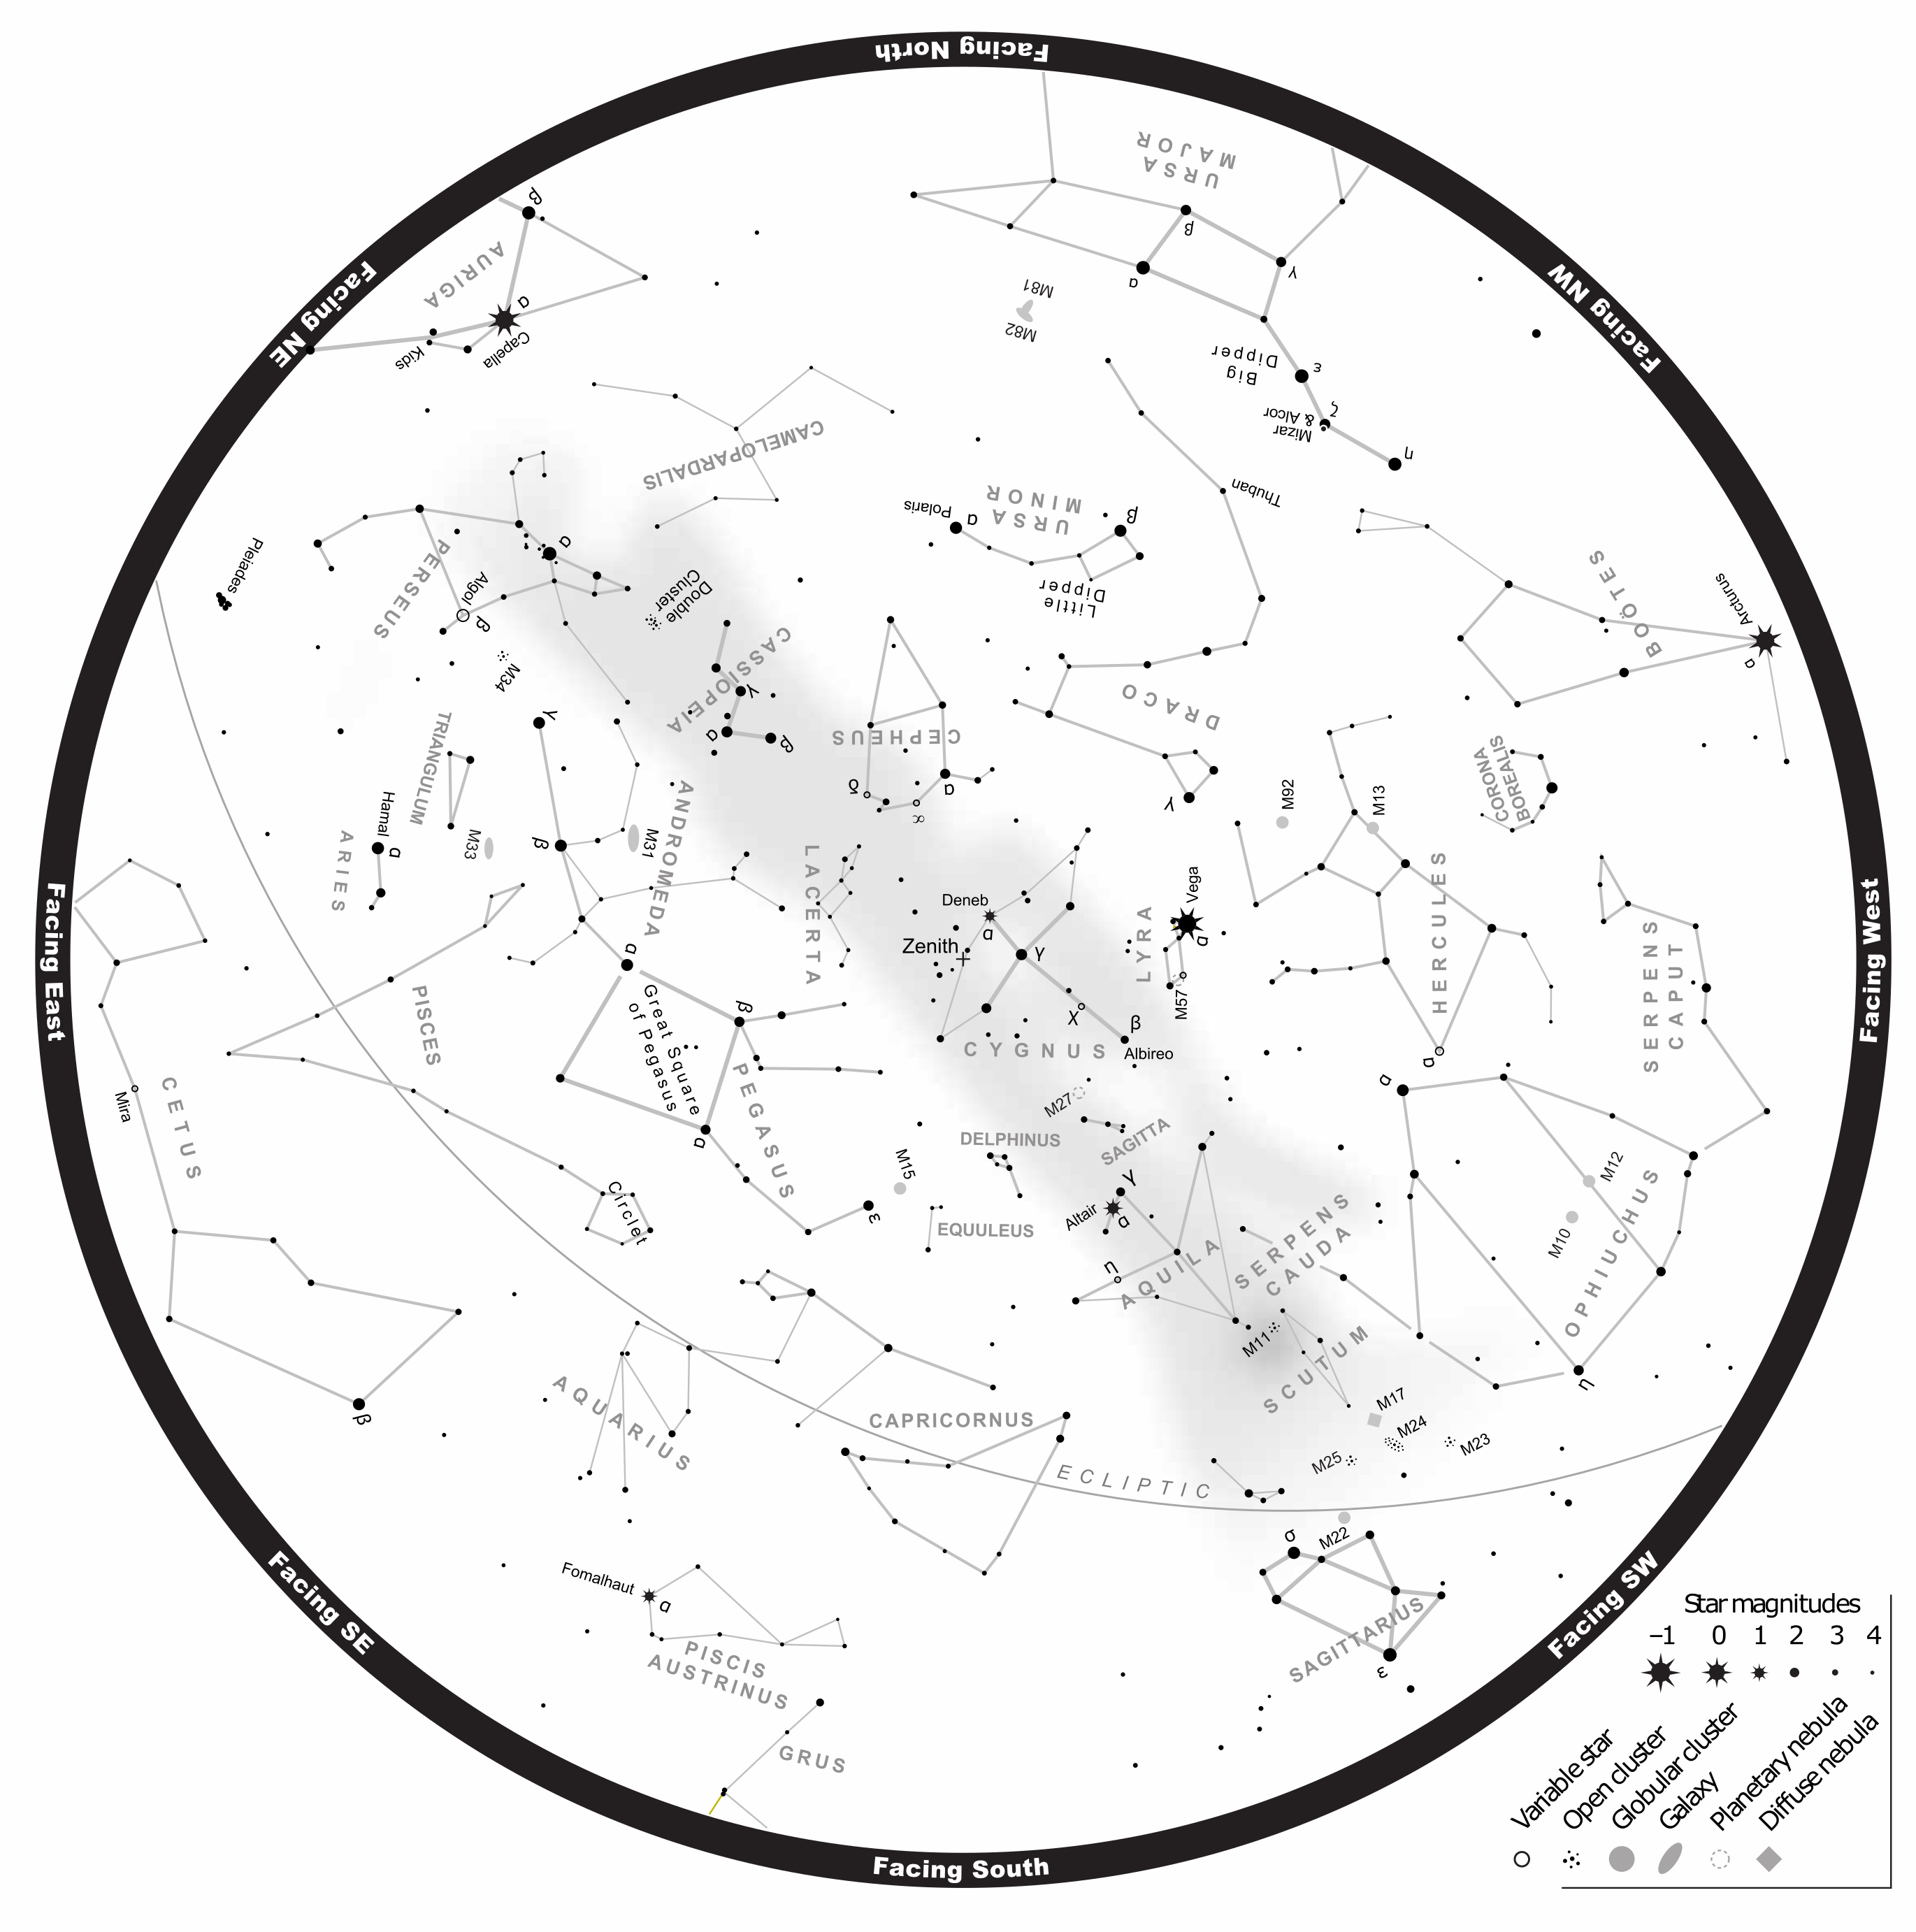
\includegraphics[width=0.9 \linewidth]{sep-oct.png}
    \caption{Sep/Oct Night Sky View for latitude $40^\circ$ N}
\end{figure}
\clearpage
\begin{figure}
    \centering
    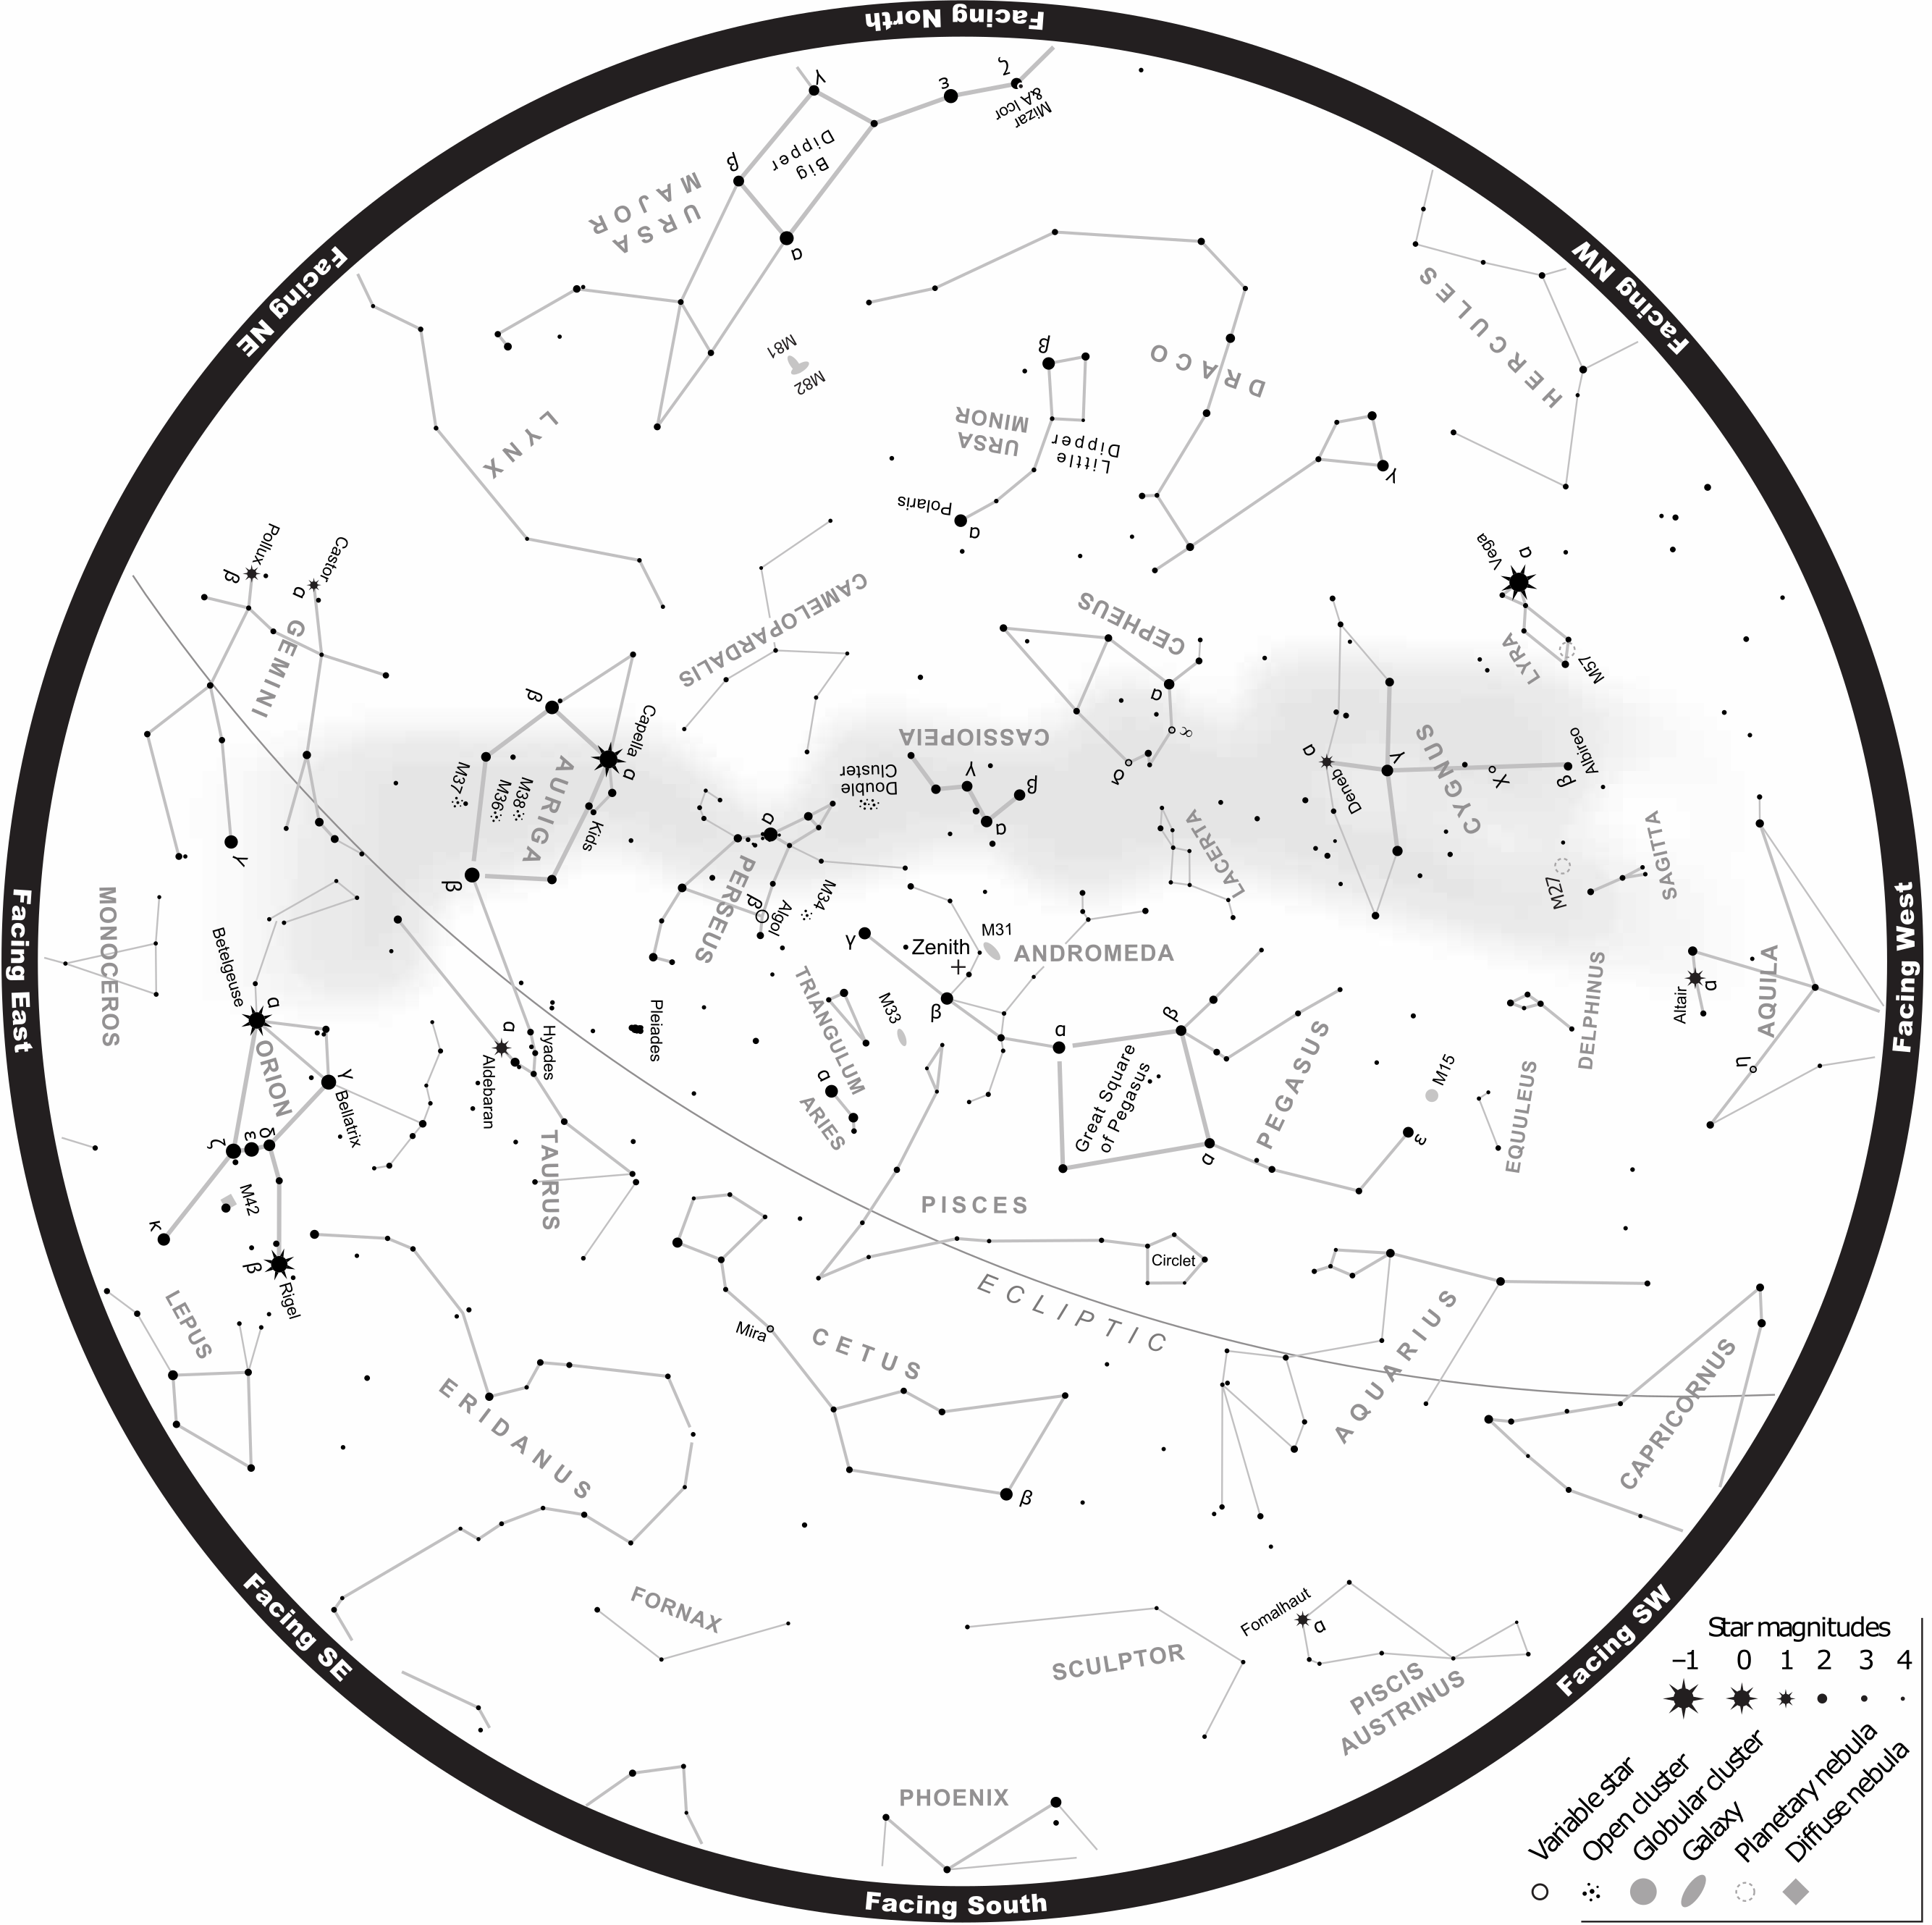
\includegraphics[width=0.9 \linewidth]{nov-dec.png}
    \caption{Nov/Dec Night Sky View for latitude $40^\circ$ N}
\end{figure}

\clearpage
\section{Celestial Navigation}
Celestial navigation has a rich and interesting history. The navigator would use ‘sights’, or angular measurements taken between a celestial body (e.g., the Sun, the Moon, Polaris, or one of 57 other navigational stars and planets) and the visible horizon to locate one’s position in the world, on land
as well as at sea.

\begin{figure}[H]
	\centering
	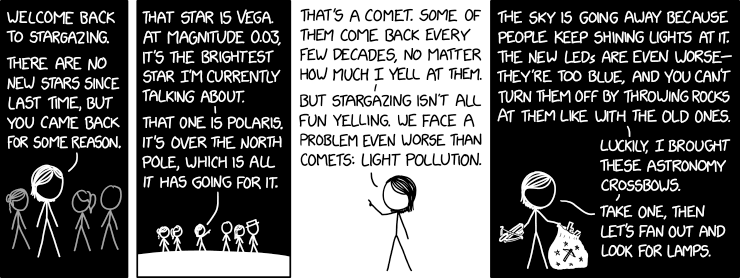
\includegraphics[width=0.9\linewidth]{navigation.png}
\end{figure}

 Let us explore a simple application of Celestial Navigation using our wrist watch. To use our watch as a compass in the northern hemisphere, hold the watch horizontal and point the hour hand at the Sun. The halfway mark between the hour hand and the twelve o’clock mark is south. For example, if it is 8 o’clock, point the 8 on the watch face at the Sun. South would then be at the 10 o’clock position. If it is 4 o’clock, point the 4 on the watch face at the Sun. South would be in the 2 o’clock position.

\subsection{Naked Eye Observation}

\textsc{\textbf{Practice Questions}}
\begin{enumerate}
	\item \textbf{Name the constellations where the Milky Way passes through that are visible from Northern and Southern hemisphere}\\
	The rotational Galactic Center of the Milky Way lies in the direction of Sagittarius, with the glowing band of hazy light then stretching all the way across to its anticenter in Auriga, before returning back to Sagittarius. From Earth, stargazers can see 30 constellations contained in this region of sky, some of which only faintly touch the region.\\
	
	- \textsf{Northern}: Monoceros, Canis Major, Orion, Gemini, Taurus, Auriga, Perseus, Cassiopeia, Lacerta, Cepheus, Cygnus, Vulpecula, Sagitta, Aquila, Serpens, Sagittarius, Scutum, Ophiuchus, Scorpius.\\
	
	- \textsf{Southern}: Norma, Lupus, Ara, Circinus, Triangulum, Crux, Musca, Carina, Vela, Pyxis, Puppis.
	

	\item \textbf{Write down any five constellations that lie on current celestial equator}\\
	- Virgo (Vir), Serpens (Ser), Ophiuchus (Oph), Aquila (Aql), Aquarius (Aqr), Pisces (Psc), Cetus (Cet), Libra (Lib), Hercules ( Her), Scutum (Sct), Delphinus (Del), Equuleus (Equ), Pegasus (Peg).
	\item \textbf{How to find/point at the vernal equinox?}\\
	- The vernal equinox is located slightly south of the circlet of Pisces. There is no bright star near its exact location hence it can be identified only through practice.
	\item \textbf{In order to know your latitude from stargazing alone, what other piece(s) of information do you need?}\\
	- Stars' altitude and declination.
	
	\item \textbf{Which of these stars cannot be observed by an observer at certain location?}\\
	
	\textsf{Circumpolar Stars}\\
	
	This question relies on your comprehension of the night sky and rough idea of where the major stars are located. A concept introduced by this question is of circumpolar stars: they are stars that either never set or never rise. As the question asks the star that cannot be observed, it means that it asks for the lower circumpolar stars(stars that never rise) for an observer at certain location.
	The only challenge is to realize that lower circumpolar stars peak at an altitude of $\delta+ 90^\circ -\phi$,
	where $\delta$ is the declination of a star and $\phi$ is the latitude of the observer. The condition for lower
	circumpolar stars would be that this altitude $< 0^\circ$. Therefore, the condition becomes $90^\circ + \delta <\phi$.
	
	
	\item \textbf{Give some practical advice for maximizing the number of meteors observed from a meteor shower during a short (3-4 hour observation session). Be specific and detailed.}\\
	
	- Observe during the peak night(s) of the specific shower!\\
	- Observe from a dark location, preferably when the Moon is not up. This is so as to see as many meteors as possible\\
	- Do not use a telescope/binoculars. Rather, just lie back and scan a large patch of sky (the larger the better) or\\
	- In the Northern Hemisphere, where must one point the polar axis of the equatorial mount towards, such that moving the telescope in Right Ascension will most precisely mimic the motion of the sky over the course of a night?\\ 
	- Generally, observe after local midnight as Earth would usually be moving into the stream of meteors then.\\
	- If possible, observe when the radiant of the shower has a high altitude.
	\item \textbf{In the constellation Crux, the} $\alpha\,, \beta, \,\gamma$ and $\delta$ \textbf{stars are named in which order?}\\
	- Clockwise
	\item \textbf{During an overnight observation session in December, a local astronomy club painstakingly recorded its observations. However, those notes ended being mixed up with observation logs from previous months. Which of the following objects is unlikely to have been observed during this December night?}\\
	
	- [Options] \\
	A. {\color{red} Lagoon Nebula (M8) in Sagittarius}\\
	B. Orion Nebula (M42) in Orion\\
	C. The Double Cluster (C14) in Perseus\\
	D. The Andromeda Galaxy (M31) in Andromeda\\
	E. Praesepe (M44) in Cancer
	
\item \textbf{On a winter evening, Aquila the Eagle is found to be setting. You are given that Altair has a right ascension of $19^h52^m$ and a declination of $+8^\circ55'25''$. Assuming that you are on the equator, what is the local sidereal time?}\\

- Sidereal time is calculated from the hour angle + RA of a particular object, where the hour angle is the number of hours after the object has passed the meridian. In other words if 0h is the local meridian, 18h would be at the western horizon. In this case, it is given that 19h52min is at that horizon. This means that the correct local sidereal time is 1h52m. 

\item \textbf{Filters are often used in practical astronomy for image enhancement, especially when imaging deep-sky objects as they appear very dim even through a telescope. When imaging an emission nebula, which color/combination of filter(s) can be used to minimise light from background sources, thus allowing the nebula to stand out better?}\\

- An emission nebula emits light that is dominated by the H-$\alpha$ spectral line (657 nm) of the Balmer series (ionized hydrogen emission). Hence, an emission nebula appears red. To enhance the image, one should minimize light from other background sources (non-red light) to enter the eye. Hence,
one should use a red color filter to allow the nebula to stand out more.Yellow filters are generally used when trying to look at the yellow dust tails of comets and not DSOs. Stacking all of the filters listed defeats the purpose of using a color filter, which is to expose the sensor to light of a
certain wavelength (color).

\item \textbf{For an observer in the Northern Hemisphere, how does the right ascension of the Sun change from the start to the end of Summer?}\\ 

\textit{NB: we define the start of a season by its corresponding equinox/solstice. So the summer solstice marks the start of Summer.}\\

- Recall that during the northern vernal equinox, the Sun is at 0h by definition. The right ascension of the sun increases as the season progresses. Further, after 1 season, the Earth would have moved along 1/4 of its orbit, leading to From 6h to 12h.
\item \textbf{Suppose your latitude is $45^\circ$ N. What is the Sun's elevation above the southern horizon at noon on the summer solstice?}\\
- The celestial equator is tilted at an angle equal to your latitude from the zenith. In this case, the celestial equator is $45^\circ$ from your zenith and therefore $45^\circ$ above the southern horizon. The Sun is $23.5^\circ$ above the celestial equator on the summer solstice. Therefore the Sun is $23.5^\circ+ 45^\circ= 68.5^\circ$ above the southern horizon.

\item \textbf{Estimating the Local Sidereal Time (LST) from Star Chart.}\\ 

\textsf{Method 1: Using RA of known object and estimating LHA to obtain LST}\\

From the definitions of the following variables, the following equation relates LST, RA at meridian and local hour angle (LHA),
$$LHA_{\rm obj}=LST-RA_{\rm obj}$$
Then, find an object with known RA, and estimate its LHA. For an object on the meridian, $LHA = 0$. For rising and setting objects, $LHA < 0$ or $LHA > 0$ respectively.\\

e.g. Arcturus has a RA of $14^h15^m$; it is estimated to have crossed the meridian (LHA) about 30 mins ago, i.e. $LHA_{\rm Arcturus} = 0^h30^m$.

Hence, $LST=LHA_{\rm obj}+RA_{\rm obj}=14^h15^m+ 0^h30^m \approx \mathbf{14^h45^m}$.\\

\textsf{Method 2: By first principles, definition of LST}\\

By definition, the $LST = LHA_{\rm Vernal \;Equinox}$, and $RA_{\rm Vernal\; Equinox} = 0^\circ$.\\

In a tropical (calendar) year, there are 365.25 solar days, but 366.25 sidereal days. By definition, \textbf{at local noon} on the day of Vernal Equinox (usually around March 20-21), the vernal equinox is at the local meridian everywhere, thus $LST = 0^h$.\\

Thus, the $LST$ at local noon every day after that increases by a small amount equal to the time required for the Earth to rotate an extra small angle due to its orbital motion, i.e. for each complete solar day the Earth completes a small fraction of the extra sidereal day. This amount is,
$$\Delta LST=\frac{1\; day}{366.25\; day}\times 24^h00^m= 3.93^m=3^m56^s$$

If we take January 28, approximately 10 months and 7 days after Vernal Equinox (there is inaccuracy introduced here as each month is not of equal length),
$$LST_{\text{noon of 28 Jan}}=\left(\frac{10}{12}\times 365.25+7 \right)\times 3^h56^m= 1197^m=20.40^h$$

If we do have a calendar, we can get a more accurate calculation, with 313 days between March 21 and January 28
$$LST_{\text{noon of 28 Jan}}=313\times 3^h56^m=1231^m=20.51^h$$
 
Now if we know time when any starchart is taken, Suppos the starchart was taken at 06:15 UTC, i.e. 6.15am at the Greenwich
Meridian,
$$LST_{\text{6.15 am on 28 Jan}} \approx 20.51^h-(12^h-6.25^h)=14.76^h \approx \mathbf{14^h45^m}$$

\item \textbf{Estimating the Local Time (LT) from Star Chart.}\\ 

For this you must know coordinates of a star lying on Celestial Equator. Recall that Orion lies along the celestial equator – and that one notable feature of the Belt of Orion are the declination of the belt stars, that is, their declination is close to $0^\circ$.\\

As an estimate, we take Mintaka’s declination to be $0^\circ$, such that it would culminate at the zenith (centre of the starchart) when the local sidereal time is equal to its right ascension. Now estimate weather Mintaka is to the /east/west of the local meridian, i.e. if it has already culminated and thus its hour angle will be $HA>0$. Thus, we measure Mintaka's distance from the centre of the starchart (zenith), to estimate its hour angle, d= X cm. Then the fraction outward from the centre of the starchart of radius is, $f=d/r$.

Then, to a first approximation, ignoring distortion from the stereographic projection, the hour angle $HA$ of Mintaka from the zenith is approximately, $HA= 90^\circ \times f$. Then the local sidereal time at the time of the starchart is (right ascension of Mintaka $\alpha=5^h 33^m$) 
$$LST=HA+\alpha$$

Let's take a star chart  that is dated 11 Mar, close to the vernal equinox 21 March, we can take the $LST_{0000}$ at local solar midnight as approximately $12^h-10\times 4^m= 11^h0^m$.\\

Then, to find the local sidereal time at local civil midnight, we need to introduce a correction as Observer's timezone (UTC+LT) is not in alignment with its longitude ($\lambda$),
\begin{align*}
	LST_{0000}'&=LST_{0000}-\Delta LST\\
	&=LST-\left(LT-\frac{\lambda}{360}(24^h)\right)
\end{align*}

Therefore, the time before midnight $\Delta T$ is simply the difference in the local sidereal times at the time of the starchart and at local civil midnight, 

$$\Delta T=LST_{0000}'-LST$$

Therefore, the local time of the star chart is $0000h -\Delta T =$ \textbf{ANSWER}. 

\item \textbf{Estimating the position of the Moon on certain local time on Star Chart after certain days.}\\

At the same local (civil) time on the \textbf{next day}, the night sky would have rotated westward by an amount approximately $4^m$ in RA.\\

However, due to the Moon's orbital motion about the Earth (anti-clockwise), it moves eastward relative to the fixed stars and its RA increases by approximately,
\begin{align*}
	\Delta RA&=\frac{360^\circ}{T_{\rm sid}}\\
	&=\frac{360^\circ}{27.3\; days}\\
	&=13.19^\circ /days\\
	& \approx 53^m/day
\end{align*}
Since the Moon's orbital plane is similar to the rest of the planets, it will thus appear eastward along the ecliptic by about 50 mins.

\item \textbf{Star-trails} Your task in this problem will be to take a photo of star-trails in the sky (stars) they draw due to the rotation of the Earth around its own axis. You can use either method to do this-- several shorter exposures, which you then combine into a single image using appropriate software, or taking one long exposure.\\

a) Take a photo of the star-trails so that the image contains the North Pole. Try to be as long as possible so that arcs form, the corresponding hour angle should definitely exceed $0^h10^m$. Describe in detail the procedure taking a picture. Record the time and place of acquisition, the length of individual exposures and parameters in the solution camera. Attach a printed photo in inverted colors to your solution.\\ 

b) What curves do the stars plot in the photograph depending on the declination $\delta_\ast$ of the star and also on
declination $\delta_c$ of the center of the frame? Justify your answer.\\

{\color{blue}
To solve this problem, we will assume for simplicity that the rays are coming from infinity as it passes through the lens does not change direction when passing through the optical center. Then it is clear that such rays from a given star describe the mantle of a cone during the day
with an apex angle of $180^\circ - 2\delta_\ast$, the axis of which intersects the plane of the camera sensor at an angle
$\delta_c$. The trajectories of the stars in the image will therefore be conic sections. If the star never sets
below the sensor plane $(|\delta_\ast-\delta_c|> 90^\circ)$, this is generally an ellipse (in the special case, when the world pole is in the center of the image, ie. $\delta_c = 90^\circ$, the stars will draw circle). If the lower culmination of the star occurs in the plane of the sensor, it is a parabola  $(|\delta_\ast+\delta_c|=90^\circ)$. If the star falls below the plane of the sensor (but also rises above
the plane of the sensor, ie.  $|\delta_\ast +\delta_c|< 90^\circ$ and  $|\delta_c- \delta_\ast|< 90^\circ$), it is generally a hyberbola. And in the special case when we have $\delta_\ast = 0$, the cone degenerates into a plane. Stars of the world therefore, the equator draws a line in the image.\\

Note: Star trails start becoming visibly apparent when a source that covers 1px stretches out to span 5px in any direction}
\end{enumerate}

\clearpage
\subsection{Telescope Aided Observation}
\textbf{1. Eyepiece}\\ 

Lens placed near the focal point of the telescope.\\
\textit{Determines:} magnification, apparent FoV, true FoV, and other specifications. Each eyepiece has a focal length just like the telescope.\\


\textbf{2. F-Number}\\ 

Telescopes are often described by both their aperture size and f number. The f-number is the ratio of the focal length of the main lens or mirror to the aperture. In astronomy, as in photography, the aperture ratio is often denoted by $f/n$ (e. g. $f/8$), where $n$ is the focal length divided by the aperture. For fast telescopes this ratio can be $f/1. . . . f/3$, but usually it is smaller, $f/8. . . . f/15$. These specifications are important because the brightness, size, and clarity of the image produced by a telescope depend on the aperture and focal length of its main lens or mirror. For example, a “150-mm (6-inch), f/8 reflector” means the primary mirror is 150 mm (6 inches) in diameter and has a focal length of 1200 mm (8 $\times$150), or 48 inches (8$\times$6).\\

If the aperture ratio is large, near unity, one has a powerful, ``fast'' telescope; this means that one can take photographs using short exposures, since the image is bright. A small aperture ratio (the focal length much greater than the aperture) means a ``slow'' telescope.\\

\textsf{\textbf{Question}} A special telescope features a 3x optical scope  with a diameter of 25mm, and a length of 120mm. Find the f-number of the scope.\\

\textbf{3. Magnification}\\

So for a given telescope, changing the eyepiece to another with a lower focal length will increase the magnification. 

$$\text{Magnification}=\frac{\text{Telescope focal length}}{\text{Eyepiece focal length}}=\frac{\text{Aperture}\times \text{Focal Ratio}}{\text{Eye Piece Focal Length}}$$ 

\begin{figure}[H]
	\centering
	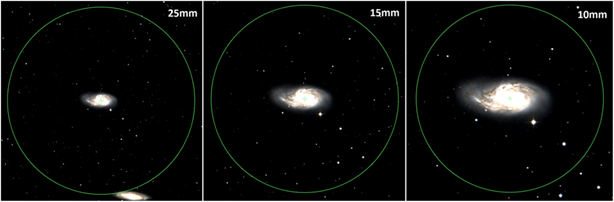
\includegraphics[width=0.9\linewidth]{tel_magnify.png}
\end{figure}

\clearpage 
\textbf{4. Field of View}\\

In general, the field of view (FOV) describes the area of a target (measured as an angle from the location of viewing) that can be seen on the chip of a CCD-camera or when looking through an eyepiece.\\

\underline{\textsf{Equation of FOV}}\\

\begin{figure}[H]
	\centering
	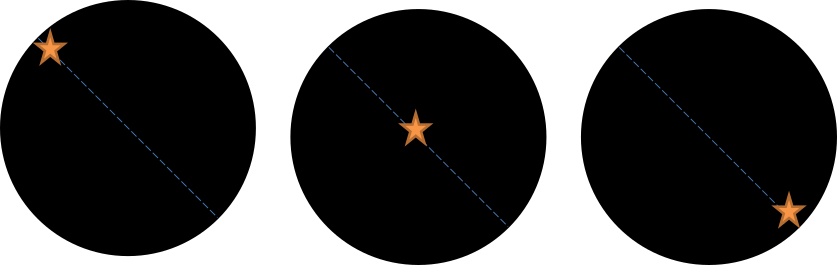
\includegraphics[width=0.9\linewidth]{FOV1.png}
\end{figure}
{\color{red}
	$$\text{FoV[deg]}= \omega \times t \times \cos(\text{declination})=\frac{360^\circ}{23^h56^m4^s.1}\times t\times \cos\delta$$}

If the star passes through the chord of the field of view, you can measure the magnitude of the central angle, which rests on this chord. $t$ - is the time during which the star passes through this chord. Then this chord $= vt \times \cos\delta $. The same chord $=a\cdot \sin\frac{\gamma}{2}$. 

\begin{figure}[H]
	\centering
	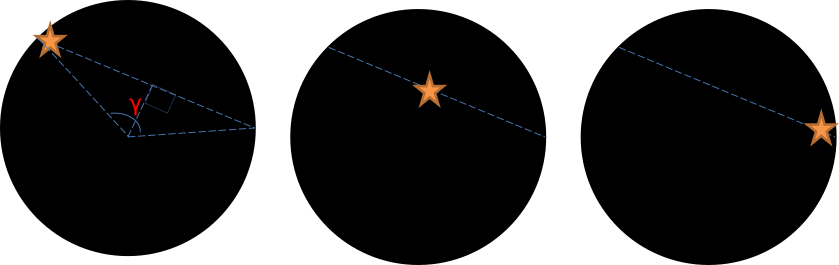
\includegraphics[width=0.9\linewidth]{FOV2.png}
\end{figure}

\textsf{Actual/True field of view (TFOV):} the angular size of the amount of sky that can	be seen through an eyepiece when used with a particular telescope, producing a specific magnification. It is typically between one tenth of a degree, and two degrees.\\ 

\textsf{Apparent field of view (AFOV):} it is a measure of the angular size of the image viewed through the eyepiece, in other words, how large the image appears (as distinct from the magnification). This is constant for any given eyepiece of fixed focal length, and may be used to calculate what the actual field of view will be when the eyepiece is used with a given telescope. The measurement ranges from 30 to 110 degrees.\\

If the apparent field of view is known, the actual field of view can be calculated from the following approximate formula:
$$\text{TFOV}=\frac{\rm AFOV}{M}$$
For a telescope with focal length of $f$, object image size of $d$,
$$\text{AFOV}=2\cdot \tan^{-1}\left(\frac{d}{2f}\right)$$ 

\begin{figure}[H]
	\centering
	\includegraphics[width=0.4\linewidth]{FOV.png}
	\caption{Same magnification but different AFoV and TFoV}
\end{figure}

\textsf{\textbf{5. Planetary (color) filters:}} Colour filters are mostly used to enhance the colour contrast differences between surface features on the moon or planets. The filters screw into a standard eyepiece barrel. The contrast differences are subtle and some observers report little or no observable differences. It may take patience and experience to recognise the differences.

{\color{blue} UHC} \quad Ultra High Contrast filter. Increases the contrast of planetary and emission nebulas.\\
{\color{blue} OIII} \quad Oxygen-III filter. Similar to UHC, but higher contrast on certain nebulas.\\
{\color{blue} H$\beta$} \quad Hydrogen Beta filter passes a particular colour of hydrogen light found in certain nebulas.\\
{\color{blue} Polariser} \quad Darkening the moon and enhancing contrast on the planets.\\
{\color{blue} IR pass} \quad Infrared pass filter is useful for getting steady views of the planets because IR is less disturbed by the atmosphere.\\
{\color{blue} Light pollution} \quad A filter to increase contrast of objects when observing from
urban areas. Darkens the sky by blocking street-lights whilst passing light from other colours.\\

\textbf{6. Finderscope}\\

Regardless of what kind of finder you are using you will have to align it with the telescope. The procedure is fairly simple and is best done during the day. The key thing is that you are aligning the finder to the telescope and not the other way around.\\

You want to do this during the day using a fixed land object. At night the things in the sky are moving which makes it more difficult to get the alignment correct.\\

During the day, set your telescope so that you can see a distant object, at least 1/4 mile away and farther is better. I prefer the cross arms on a telephone or power pole. That gives me a very well defined target right where the cross arm meets the pole. But the top of a chimney, a letter on a distant sign, or something similar can work as well. This is your alignment target\\

Here are the steps to follow.

\begin{itemize}
	\itemsep0em 
	\item Using your low power eyepiece point the telescope at the target and get it centered in the field of view of the eyepiece. Ignore the finder for now.
	\item Switch to a high power eyepiece and again, get that target centered
	\item Lock the scope into position in any way you can. You don’t want it to move
	\item Look through the finder and spot the target
	\item Using the adjustments on the finder bracket adjust the finder until the target is centered in the finderscope.
	\item Go back to the eyepiece and make sure the scope has not moved. The target should still be centered
	\item Check the finder again and make any final adjustments
\end{itemize}

When the finder and the telescope both are lined up on the same point on your target, you are all set and ready to take your telescope out under the stars.

\begin{figure}[H]
	\centering
	\includegraphics[width=0.8\linewidth]{finderscope.png}
	\caption{Left: finderscope FOV and marking, Right: a typical finderscope.}
\end{figure}
\textbf{7. Telescope Mount}\\

There are two main types of telescope mount – equatorial and altitude-azimuth (``alt-az'')– with many variations.\\

\textit{Equatorial}: This type of mount has been popular, almost universal, since telescopes achieved any sort of useful size. As we have seen, the equatorial system of co-ordinates ($\alpha, \delta$) is based on the rotation of the Earth. A telescope with one axis aligned with the polar axis only needs to be driven around this axis at the sidereal rate to track astronomical objects.\\

\textit{Alt-az} mounts are the simplest telescope mounts. Advantages: Cheap and simple to operate.
Telescope moves up/down (altitude) and left/right
(azimuth). Reflecting telescopes using this mount are known as \textit{Dobsonians}. There are a couple of (minor) drawbacks to alt-az telescopes:\\

• The necessity for continuous rapid calculation of altitude and azimuth. This has been solved by the power of modern computers – so not really a problem at all.\\
• We have seen that the relationship between horizontal and equatorial co-ordinates can be expressed by two equations such as:
\[\sin a=\sin \delta \sin \phi+\cos \delta \cos \phi \cos H\]
and,
\[\sin A=-\frac{\sin H \sin \delta}{\cos a}\]

Note that, in the second equation, if the altitude (a) approaches 90◦, the azimuth (A) approaches infinity. What this means, of course, is that for an object which passes through the zenith, as it does so, its azimuth jumps instantaneously from 90◦ East to 90◦ West (or from 90◦ to 270◦). In practice, it means that for objects near the zenith, it is very difficult to transform quickly enough and accurately enough from equatorial to horizontal co-ordinates and a small patch of sky near the zenith is effectively inaccessible, even though the telescope can easily point there. Simple observing programme planning should avoid problems from this source.\\


\begin{wrapfigure}{r}{0.5\linewidth}
	\centering
	\includegraphics[width=\linewidth]{fieldrot.eps}
	\caption{Field Rotation: Alt-Az and Equatorial Mounts}
\end{wrapfigure}

\textbf{8. Field Rotation}\\

Alt-az mounts are to be avoided due to a phenomenon
known as field rotation. Field rotation occurs due to
the design of the alt-az mount. One axis, the azimuth
axis, rotates around a vertical line passing from the
center of the telescope to the zenith (left to right). The altitude axis rotates about a horizontal axis (up and down). Both axes must rotate at different rates to maintain the object in the field of view (FOV). As the Earth rotates about its axis, the central object in the field of view will remain centered but other objects in the FOV will appear to rotate with elapsed time. Field Rotation is an undesirable effect on time-exposure astrophotographs caused when an "Alt-Az" ("altitude-azimuth" or altazimuth) mount (sometimes called a "Dobsonian" or "fork mount") is used to hold and point a telescope with a camera. It is also sometimes called Frame Rotation because the objects framed by the photograph seem to have rotated while the picture was taken.\\

Let the FOV of the telescope be represented by a
square and follow the motion of Sagittarius as it
rises in the east. Because the alt-az mount can only
move around the azimuth axis and the up and down
on the altitude axis, the FOV remains fixed with the
bottom parallel to the horizon. The objects in the sky, however, are rotating around the celestial pole star, Polaris. So asterisms and binary stars appear to rotate in the FOV. An equatorially mounted telescope does not suffer field rotation because the telescope is polar aligned and the FOV does not remain horizontal as it tracks; the telescope rotates. So the FOV matches the rotation of the object and it remains in the same fixed position.\\

\textbf{Mathematical Concepts Behind Field Rotation}
Stars appear to rise in the east and set in the west, rotating about the north celestial pole star, Polaris. Rising stars will reach their highest elevation in the sky as they cross the local meridian, due south of the line between Polaris and the zenith. The altitude indicates the vertical position of the star with $0^circ$ at the horizon and $90^circ$ at the zenith. From direct observation, the following aspects are known about rate of rotation
\begin{enumerate}
	\item The maximum rate of field rotation occurs as the star passes through the zenith.
	\item The rate of field rotation is minimal when a star passes through the prime vertical at the
	horizon.
	\item Considering the azimuth only, the rate of field rotation is highest when the star passes
	through 0° (N) and 180° (S), and lowest when
	the star passes through 90° (E) and 270° (W).
	\item Regarding latitude, field rotation is highest at the Earth’s equator and non-existent at the NCP and SCP.
\end{enumerate}

\begin{equation}
	\text{Rotation Rate}= \frac{\omega_\oplus \ast \cos(\text{Latitude}) \ast \cos(\text{Azimuth})}{\cos\text{(Altitude)}}
\end{equation}
where $\omega_\oplus=4.178 \times 10^{-3}$ degrees/second; Earth’s rotation. \\

If we only consider changing the values of the
azimuth in Equation 1, the least amount of field rotation (zero) is along the prime vertical (due east or west) because east is 90° from north (cos 90°=0) and west is 270° from north (cos 270°=0). Looking toward the other directions, the maximum rate of field rotation is when the star is due south (180° from north; cos 180°=1) or directly north where cos 0°=1.

$$\text{Least ROR}_{E,W}= \frac{\omega_\oplus \ast \cos(\text{Lat}) \ast 0}{\cos\text{(Alt)}}=0;\quad \text{(Az = 90 or 270)}$$


$$	\text{MAX ROR}_{N,S}= \frac{\omega_\oplus \ast \cos(\text{Lat}) \ast 1}{\cos\text{(Alt)}};\quad \text{(Az = 0 or 180)}$$

The altitude function deals with values between
the horizon (0°) and the zenith (90°), so only considering changes to the values of the altitude in Equation 1 and using the trig values given above we get to following.
$$	\text{RoR}_{Horizon}= \frac{\omega_\oplus \ast \cos(\text{Latitude}) \ast \cos(\text{Azimuth})}{1}; \quad \text{Alt = 0}$$
so the rate depends solely on the latitude and azimuth.
$$	\text{RoR}_{Zenith}= \frac{\omega_\oplus \ast \cos(\text{Latitude}) \ast \cos(\text{Azimuth})}{0}; \quad \text{Alt = 90}$$
which is an undefined quantity and not allowed.


\clearpage
\textsc{\textbf{Practice QnA}}
\begin{enumerate}
	\item \textbf{In what situation would polar alignment be necessary?}\\
	- To track stars/to counter diurnal motion
	\item\textbf{ What is the purpose of using a finderscope?}\\
	- Find objects more easily due to larger FOV. Image is upside down and left-right inverted.
	Magnification: 6 $\times$ 30, or 8 $\times$ 50 typically.
	\item \textbf{When not in use, how should accessories (eyepieces, diagonals, binoculars, finderscopes, etc.) be stored?}\\
	- Store in dry box/Ziploc bag to combat humidity, with foam/cushion to add stability and protection.
	\item \textbf{How do you polar‐align your telescope near the equator, where Polaris cannot be seen most
		of the time?}\\
	
	- Use compass to find magnetic North for alignment of azimuthal axis, then adjust mount's elevation/altitude to Singapore’s latitude  (less accurate), or\\
	
	Drift alignment: observe North/South drift then adjust altitudinal axis, observe East/West (RA) drift then adjust azimuthal axis (more accurate).
	\item  \textbf{After assembling, if you can move the main optical tube easily, is the counter weight located at the correct or incorrect position? }\\
	
	- Correct position. The counter weight should balance with the OT, so a little force should move it smoothly. 
	\item \textbf{Why do we need to align an equatorial telescope towards the North Celestial Pole / Polaris?}\\
	- As stars revolve around Polaris every $23^h56^m$, we can use only one knob to trace the star easily.
	
	\item \textbf{Given a telescope with an aperture of 100mm and a focal length of 1600mm, when a 1.25-inch eyepiece
	of focal length 40mm is used, what is the effective magnification?}

- Telescope magnification is calculated by dividing the focal length of the telescope by the focal
length of the eyepiece. So $\mathbf{40\times}$. Again too find the magnification, we can use
$$\text{Magnification}=\frac{\text{Aperture}\times \text{Focal Ratio}}{\text{Eye Piece Focal Length}}$$

	
	\item \textbf{You would like to maximise your view of the Pleiades star cluster ($110'$) in your eyepiece. Given the following details of your telescope, which eyepiece should you choose? (1 inch = 2.54cm)}\\
	
	\textbf{Telescope: 5-inch aperture, f/6}\\

{\color{blue}  Let the eyepiece focal length be x mm and apparent field-of-view be $y^\circ$.
	
focal length = (aperture size) $\times$ (focal ratio) = $5 \times 2.54 \times 6 \times 10 = 762$ mm.\\

$$\text{magnification}=\frac{\text{focal length of telescope}}{\text{focal length of eyepiece}}=\frac{762}{x}$$.
$$\text{true field-of-view}=\frac{\text{apparent field-of-view}}{\text{magnification}}\times 60= \frac{y}{\text{magnification}}=\frac{60xy}{762}\; \rm arcminutes$$

Calculate for each option with the different values of $x$ and $y$. This gives 35 mm focal length, $40^\circ$ apparent field-of-view.}
	
\item \textbf{You brought out your club’s $6''$ F/6 Newtonian telescope to observe M6. With a quick search you realise M6 is 2$5'$ in angular diameter. Which eyepiece would you attach to the telescope to maximise your view of M6 while still ensuring the whole of M6 can be seen in the eyepiece? (FL=Focal length,
AFOV= Apparent field of view, 1 inch = 2.54cm)}	\\

\textit{Options}\\
A. FL: 32mm, AFOV: 50$^\circ$\\
B. FL: 40mm, AFOV: 40$^\circ$\\
C. FL: 13mm, AFOV: 50$^\circ$\\
D. FL: 7mm, AFOV: 60$^\circ$\\
E. FL: 4mm, AFOV: 70$^\circ$\\

Focal length = aperture $\times$ Focal ratio = $(6\times 2.54) \times 6 \times 10  = 914.4$ mm.\\
$$\text{Magnification} =\frac{914,4}{x}$$
\begin{align*}
	\text{TFOV}=&\frac{\rm AFOV}{M}\\
	\text{TFOV [in arcmin]}=&\text{TFOV [in degrees]} \times 60\\
	>& 25'
\end{align*}

Option \textbf{D} matches the perfect condition.

\item \textbf{The Celestron C8 is a Schmidt-Cassegrain reflective telescope with a focal ratio of 10 and a diameter of 203.2 mm. Using an objective lens (eyepiece) with a focus of 25 mm, a circular squirrel with a diameter of 25 cm fills the field of view completely. Assuming an apparent field of view of $50^\circ$.}\\

The focal length of the telescope is 203.2 cm. Using the focal ratio, we can infer that the focus is ten times longer, i.e.
2032 mm.\\

Using, $FoV =\dfrac{50}{M}=50\times \dfrac{f_{oc}}{f_{ob}}=37'$.\\

The distance from the squirrel to the observer is 2328 cm. The distance can be obtaind using trigonometry. Specifically, $d=\dfrac{h}{\tan \alpha}$, where $\alpha = 50^\circ$.\\

The resolving power is $0.68''$ from $\theta =1.22\dfrac{\lambda}{D}$. \\

\item \textbf{The Celestron Advanced VX Y Go-To Reflector Telescope has an $Y''$ optical tube assembly with specification f/5, where Y is an unknown value. The focal length of the optical tube is 1016 mm. Two eyepieces, one with diameter 8 mm and another with diameter 25 mm were provided. Determine the minimum size of a crater on the Moon that can be resolved by this telescope. Assume light of wavelength 550 nm.}\\

The aperture diameter is determined by
$$D=\frac{f}{N}=\frac{1016}{5}= 203.2 \; \rm mm$$
Using the formula for the Rayleigh criterion $\theta =1.22\dfrac{\lambda}{D}$ with $\lambda= 550$ nm, $D = 203.2$ mm, we get that the minimum angle that can be resolved is $0.0001892^\circ$.\\

Using $s = r\theta$ and the Earth-Moon distance of $3.843\times 10^8$ m, we see that the minimum distance on the Moon that can be resolved is
$$s=5.843\times 10^8 \times  \frac{0.0001892}{360}\times 2\pi =1.27\; \rm km.$$
\end{enumerate}

\textbf{\textit{Try Yourself}}
\begin{enumerate}[P1.]	
\item  Student A has just received a telescope from her professor. Her professor had performed some measurements on the telescope, and told her that it has an effective focal length of 1800mm, with an aperture of 90mm. Student A next chooses to use a 5 mm Plossl eyepiece, with an advertised apparent field of view (AFOV) of $40^\circ$.
\begin{enumerate}[i.]
	\item Calculate the f/ratio of this scope
	\item Calculate the resultant magnification that this setup provides
	\item Calculate the exit pupil of this setup.
	\item Calculate the true field of view (TFOV) for this setup.
	\item Is this setup good for deep sky astrophotography? Justify your answer.\\
	(Hint: Think about highest useful magnification. Also, an average dark adapted human eye has an entrance pupil of about 7mm)
\end{enumerate}

\item  Upon further investigation, Student A discovered that a 3X Barlow lens had been left in the telescope’s visual back. She thus removed the Barlow. She also changed the eyepiece to a 10mm Nagler, with an advertised $80^\circ$ wide-view AFOV.\\

Calculate the new effective focal length, f/ratio, magnification, exit pupil and TFOV.

\item Chuan Ming is observing an unknown bright star through a refractor on an equatorial mount with a
2-degree true field-of-view. He observes that the star takes roughly 9.23 minutes to fully cross the
diameter of the eyepiece field of view. Estimate the declination of the star. Assume the star is in the
northern hemisphere.

\item A curious astronomer has observed two stars while they have been passing across the very center of telescope’s field of view at the same time interval. One day, he noticed one of them rising and another setting simultaneously. Show that the stars will appear in exactly opposite directions on the horizon. Ignore any atmospheric effects.
\end{enumerate}


\clearpage
\subsection{Telescope Long Questions}

\subsubsection{Liquid Mirror Telescope}

A relatively inexpensive way to make a parabolic mirror involves rotating a liquid around in a circle.
Such a construction is called a liquid mirror telescope. See this video by \textit{Action Lab} - \url{https://www.youtube.com/watch?v=s0sQYAWSHzU}\\

In this problem, we explore the physics of the liquid mirror telescope. Consider a liquid rotating around in a cylinder with radius $r$ at an angular velocity $\omega$ around the cylinder’s axis. For the following parts, you are to ignore effects of surface tension
\begin{enumerate}[a.]
	\item Let $y(r)$ represent the height of the liquid surface at a radial distance $r$ from the axis of rotation. By considering the forces acting on a small element on the surface of the container, determine the gradient $\dfrac{dy}{dr}$ as a function of $r$.
	\item Determine an equation for the height of the mirror surface with radial distance r from the cylinder's axis. Should you need, $$\int ax^n dx=\frac{ax^{n+1}}{n+1}+C$$
	\item \textit{The Large Zenith Telescope} had (it is no longer in use) a diameter of $6.0$m and a rotation period of 8.51s. Determine the focal ratio and plate scale of this telescope.\\
	Should you not have obtained an answer to the previous parts, you may use 12.0m as the focal
	length of the \textit{Large Zenith Telescope}.\\
	\textbf{Hint:} The Cartesian equation of a parabola is given by $y = 4fx^2$.
\end{enumerate}
\fbox{\begin{minipage}{44em}
\textbf{a.} Consider an element along the surface of the mirror, a radial distance $r$ from the centre
The buoyant force (green arrow) must provide for the centripetal force, and also counter the gravitational force on the element
$$\frac{dy}{dr}=\tan \theta=\frac{\sin\theta}{\cos\theta}=\frac{m\omega^2 r}{mg}$$

\textbf{b.} 
$$\frac{dy}{dr}=\frac{m\omega^2 r}{mg}$$
$$\int_0^r (\omega^2r/g)dr= \frac{\omega^2 r^2}{2g}$$
It is technically not required to integrate; so long the participant has a qualitative understanding of an integral as the area under a graph, the
answer can be arrived at through finding the area under the straight line graph with gradient $\omega^2/g$.\\

\textbf{c.} For a parabola, we have $x^2=4fy$ where $f$ is the focal length. Rearranging, $y=\dfrac{1}{4f}r^2$,
$$\frac{1}{4f}=\frac{\omega^2}{2f}\rightarrow f=\frac{g}{2\omega^2}=9.0\; m$$
$$\frac{f}{D}=\frac{9}{6}=1.5$$
$$p=\frac{206265}{9m}=22.9''/mm=23''/mm$$
\end{minipage}}

\subsubsection{Alt-azimuthal Mount}
In the Poland during IOAA at a site with latitude = $50^\circ$, an observer centered his altazimuth-mounted telescope at a star with declination $\delta = -18^\circ$ at the moment of its culmination in the South. He then started an automated motion of the telescope along its vertical axis with a period of one sidereal day $T= 86 164$ s. Half an hour later ($t = 1800$s), he came back to the telescope and found that the star had left the field of view.\\

The observer is now interested to know if he can observe the star after replacing the eyepiece so that the field of view has a diameter $d= 0.5^\circ$, and in the case that he cannot, if he could bring the star back into the field of view by moving the telescope along exactly one axis (either vertical or horizontal). Note that the astronomical azimuth is measured from the North eastwards.

\begin{enumerate} [a.]
	\item Determine the horizontal coordinates $a_D, \; z_D$ (azimuth and zenith distance) of the center of the field of view of the telescope at $t = 1800$s after initiating the telescope motion. Express the result in degrees.
	\item Determine the horizontal coordinates $a_H,\; z_H$ of the star at $t = 1800$ s after initiating the telescope motion. Express your answer in degrees.		
	\item Is it possible to observe the star after replacing the eyepiece?
	\item Can the observer bring the star back into the field of view by moving the telescope along exactly one axis? If so, along which axis (either vertical or horizontal) does the telescope need to be moved?\\
	Hint: For $a,b\neq 0$, the function $f(x)=a\sin x+b \cos x$ attains its minimum/maximum in the open interval $x \; \epsilon \; (0,180^\circ)$ exactly at the point $x=\arctan\left(\frac{a}{b}\right)$
\end{enumerate}

\fbox{\begin{minipage}{44em}
\textbf{a.} The zenith distance $z_D$ did not change with the displacement of the telescope and is $z_D = \phi - \delta = 68^\circ$. The azimuth has the value $a_D =\dfrac{t}{T} \cdot 360^\circ = 7.5^\circ$.	\\

\textbf{b.} For this we will use the spherical triangle $SZH$, where $S$ is the north celestial pole, $Z$ is the zenith and $H$ is the observed star. We determine the zenith distance from $H$ of the star using the cosine theorem for the sides
$$\cos z_H = \cos |SH| \cos |SZ| + \sin |SH| \sin |SZ| \cos \alpha,$$	

where $|SH| = 90^\circ -\delta$ is the angular distance of star $H$ from the north celestial pole, $|SZ| =90^\circ - \phi$ is the zenith distance of the north celestial pole, and $\alpha  =\dfrac{t}{T} \cdot 360^\circ$ is the angle by which the sky has apparently rotated around the north celestial pole in time $t$. Thus,
$$z_H = \arccos (\sin \delta \sin \phi + \cos \delta \cos \phi \cos \alpha)= 68.3^\circ $$
We determine the azimuth $a_H$ of the stars from the sine theorem
$$\frac{\sin|ZH|}{\sin\alpha}=\frac{\sin|SH|}{\sin(180^\circ -a_H)} \Rightarrow \arcsin \left(\frac{\cos\delta \sin\alpha }{\sin z_H}\right)=7.70^\circ,$$

where $|ZH| = z_H$ is the zenith distance of the star $H$. It should be noted that the previous equation has two solutions on the interval $[0, 180^\circ]$. However, since $t\ll T$, only one solution on the interval $[0, 90^\circ]$ makes physical sense. Formally, it is possible to verify this by substituting into the cosine theorem for the side $SH$, whose opposite interior angle is $180^\circ- a_H$.
\end{minipage}}
\clearpage
\fbox{\begin{minipage}{44em}
\textbf{c.} Now that we know the azimuthal coordinates of the star $H$ and the field of view of the telescope $D$, we can determine their mutual angular distance l using the cosine theorem for the sides of the spherical triangle $ZDH$
$$l = \arccos (\cos z_D \cos z_H + \sin z_D \sin z_H \cos (a_H − a_D))= 0.36^\circ $$
Since $l > d/2 = 0.25^\circ$, it is not possible to observe the star even after changing the eyepiece.\\


\textbf{d.} Because $|z_D - z_H| = 0.32^\circ$, and therefore $|z_D - z_H| > d/2 = 0.25^\circ$, it is not possible to observe the star after moving around the vertical axis of the telescope.\\

When moving around the horizontal axis, the zenith distance $z_D'$ of the telescope changes. For the fine angular distance $l'$ between the star and the telescope, it holds
$$\cos l' = \cos z_D' \cos z_H + \sin z_D' \sin z_H \cos(a_H - a_D)$$

Since the cosine function is decreasing on the interval $[0, 180^\circ]$, we are looking for the maximum of the function
$$f (z_D') = (\sin z_H \cos (a_H - a_D)) \sin z_D' +(\cos z_H) \cos z_D'$$ 
According to the hint in the assignment, this function reaches a maximum at a point
$$z_D'=\arctan\left(\frac{\sin z_H \cos(a_H-a_D)}{\cos z_H}\right)=\arctan (\tan z_H \cos (a_H-a_D))=68.3^\circ$$
Let us emphasize that $z_D'\neq z_H$, as follows from the presence of the term $\cos (a_H-a_D)$ in the relation for $z_D'$. By re-substituting $z_D'$ into the relationship for $l'$, we get the minimum possible angular distance of the star $H$ from the center of the field of view of the telescope as it moves around the horizontal axis
$$l' = \arccos (\cos z_D' \cos z_H + \sin z_D' \sin z_H \cos (a_H - a_D))= 0.16^\circ.$$
Since $l' < d/2 = 0.25^\circ$, the observer can observe the star after moving the telescope around its horizontal axis, if he sets the center of the field of view to the zenith distance $z_D'$.
\end{minipage}}


\clearpage
\subsection{Astrophotography}
As the prices of DSLRs drop since their inception, more people now can take photographs of the night
sky. The art of Astrophotography has caught on to become a serious pastime for amateur astronomers.\\

\textsf{Photography Jargon}\\

Before we jump in, we should familiarise a little on some technical jargon that is commonly used in the
photography community. The ultimate goal of a photographer is to control the amount of light captured by the sensor when taking a photo. It cannot be too much light else the photo will come out overexposed (too bright). The converse is true too, when the camera does not capture enough light.
To achieve a good control over light, photographers concern themselves with 3 main settings:

\begin{table}[H]
	\centering
	\begin{tabular}{|c|c|}
		\hline
		\textbf{Camera Settings}                                               & \textbf{What it Controls}                                                                                                   \\ \hline
		Shutter Speed / Exposure Length                                        & \begin{tabular}[c]{@{}c@{}}The length of time the sensor is exposed to light.\\ (e.g. 1/3s, 1/1000s, 1s, etc.)\end{tabular} \\ \hline
		\begin{tabular}[c]{@{}c@{}}ISO \\ (pronounced ``eye-soh'')\end{tabular} & \begin{tabular}[c]{@{}c@{}}The Sensitivity of the sensor.\\ Higher ISO = More Sensitive\end{tabular}                        \\ \hline
		f-Number/Ratio                                                         & \begin{tabular}[c]{@{}c@{}}Aperture size of the lens.\\ Same definition with a telescope's f-ratio.\end{tabular}            \\ \hline
	\end{tabular}
\end{table}
These three settings are what a photographer uses to control the amount of light that hits the sensor.\\
	
The last setting is known as the Zoom. It controls how magnified the image will be. It is usually expressed as the focal length of the lens. (e.g., 18mm, 35mm, 120mm etc.)

\subsection{Guessing the correct Magnitude}

Conditions for comparing sight according to the Pickering method:
\begin{itemize}
	\itemsep0em
	\item a small angular distance of the comparison star from the variable star;
	\item the spectral classes of the comparison star and variable star must be adjacent on the Harvard scale of spectral classes
\end{itemize}

IDEA:
1) Choose 2 stars with known magnitudes of more or less the same brightness
2) Divide the interval between them into 10 parts (or in the Neyland method - Blazhko into any number of parts, for example, into 5)
3) Determine where the observed star is on the interval
4) By linearizing the scale, you determine the magnitude

\section{Practice Olympiad Problems}

\fbox{\begin{minipage}{44em}
		Practice problems are from Bangladesh Olympiad on Astronomy and Astrophysics (BDOAA), Singapore Astronomy Olympiad (SAO), Indian National Astronomy Olympiad (INAO), Czech Astronomy Olympiad, International Earth Science Olympiad (IESO), and International Olympiad on Astronomy and Astrophysics (IOAA). Problem setters of perspective questions are credited. 
\end{minipage}}

\subsection{How OBS Marking works}




\clearpage
\subsection{BDOAA}
From my experience as an amateur Astronomer and IOAA team leader for 5 years I came across these things student should be aware and mindful about. 
\subsubsection{2019}
On \nth{23} March, 2019, Mahmud and Fahim were observing their local sky with their IAU100 Bresser Telescope. According to their observation Mahmud made a sky map using “Your Sky” website. Now you’ve to find few things according to their map--

\begin{figure}[H]
    \centering
    \includegraphics[width=0.8\linewidth]{BDOAA_19.png}
\end{figure}
\begin{enumerate}[a.]
    \item Name the stars 1,2,3, 4, and 5 and their constellations.
    \item Draw a circle for the Circumpolar star region. [A circumpolar star is a star, as viewed from a given latitude on Earth, that never sets below the horizon due to its apparent proximity to one of the celestial poles.]
    \item If the Field of View (FOV) of this map is $80^\circ$, find the angular distance from $\alpha$ Cassiopeia to $\alpha$ Ursa Minor. [Hint: the line passes through the center of the eyepiece of the Telescope)
    \item Prove that if the right ascension of a star is equal to its altitude from one point/place then the magnitude of its longitude and declination is also equal from that point/place.
\end{enumerate}
\subsubsection{2021}
Fahim is an Astronomer who likes to observe the sky. He travels the world with his telescope. Referring to the image of the night sky at an unknown location, Fahim was observing the sky. 

\begin{figure}[H]
    \centering
    \includegraphics[width=\linewidth]{BDOAA_2.png}
\end{figure}

 On the image, answer the following questions. [For this you can use any means to copy the image then draw everything necessary with computer paint or whatever you like]
\begin{enumerate}[a.]
    \item  Identify the cardinal points.
    \item Trace out the `Little Dipper' and label it accordingly.
    \item Trace the `Great Square of Pegasus' and label it accordingly.
    \item Trace out two major complete IAU constellations that are visible (other than Cygnus, Ursa Major, and Ursa Minor).
    \item Mark the positions of two prominent nebulae that are visible and label them accordingly.
    \item Mark the positions of two prominent open clusters that are visible (except Hyades) and label them accordingly.
    \item Mark the approximate positions of two prominent galaxies that are visible and label them accordingly 
    \item Approximately, what is the latitude of this location?
\end{enumerate}


\subsection{INAO}

\subsubsection{2019}

The picture below was taken on \nth{24} December 2019, from some place in India, showing the crescent of the Moon near the horizon (the horizontal dashed line marks the horizon of the place). Field of View (FOV) of the image is $60^\circ$.
\begin{figure}[H]
    \centering
    \includegraphics[width=0.9\linewidth]{INAO_19.png}
    \caption{Negative image of certain patch of the sky on \nth{24} December 2019}
\end{figure}
Note: The images printed are colour-inverted, i.e. the bright parts of the image appear black and dark parts appear white. Thus, the black dots are stars and planet and the dark cresent is actually bright crescent of the moon.
\begin{enumerate}[a.]
    \item At which of the following times this picture may have been taken? Give justification for your answer.
    \begin{center}
    18:00 hrs,\quad 22:00 hrs,\quad 01:00 hrs,\quad 05:00 hrs. 
    \end{center}
    \item Write the names of the constellations present in the image of the sky.
    \item The map also includes a planet. Mark the planet on the map with a circle and label as `P'.
    \item A zoomed-in image of the lunar crescent is given in the answersheet. On this image mark the approximate directions to the cardinal points. [East-West-North-South] Note: You may assume the box in the answersheet has a linear angular scale along the horizon.
    \item Find approximate latitude of the place.
horizon.
\end{enumerate}

\subsubsection{2018}

\begin{enumerate}[a.]
    \item Let us say we are observing sky from a dark location and all planets are visible in the sky. Arrange the planets of the solar system in the descending order of their apparent brightness as observed from the Earth.
    \item Shinjini was observing the sky from a location on the equator on the night of 20-21 March and she made following observations in her diary.
    \begin{itemize}
        \item Today is 11 days prior to the full Moon.
        \item Saturn is seen in constellation of Sagittarius.
        \item Jupiter is seen rising at the time of the Moon set.
        \item Mars’ position was coinciding with the centre of Milky Way.
        \item Mercury set about 2 hours before the Moon.
        \item Venus was seen in the evening sky for about 2 hours after sunset.
    \end{itemize}
In the answersheet, you will find a circle which is passing through East, Zenith (point exactly above the head of the observer), West and Nadir (point exactly below the observer). Use the information given above to mark positions of the Sun, the Moon and the 5 planets on this circle at 11 am on the Vernal Equinox day (\nth{21} March). For each object, write a 1-2 line explanation stating why you think it is the correct position of the object.
\end{enumerate}


\subsubsection{2016}

The skymap below [Figure \ref{INAO16}] corresponds to sky above Nagpur ($21^\circ$ N, $79^\circ$ E) at 09:00 am on \nth{1} February 2014. If you are not used to using sky maps, it is important to note that sky map is usually seen lying down on the ground (feet to the South), facing the sky with map in your hand. Thus, East is on the left of the map and West is on the right. Answer the following questions:\\

\begin{enumerate}[a.]
    \item Mark Polaris with letter ‘\textbf{P}’.
    \item Circumpolar stars for a given place are the stars, which will never go below the horizon. Draw boundary of this region and mark it by the letter ‘\textbf{C}’.
    \item The celestial equator is just a projection of the Earth’s equator in the sky. It will be the locus of points which are equidistant from the north and the south pole. Draw the equator on the map approximately and mark it with ‘\textbf{Q}’.
    \item The ecliptic is the imaginary yearly path of the Sun in the sky. Mark this approximately on the map and mark it with ‘\textbf{E}’.
    \item Mark approximate position of the Sun on the map as ‘\textbf{S}’.
    \item Yesterday was a new moon day. Mark the current position of the moon on the map as ‘\textbf{M}’.
    \item Which star was very close to the Zenith at 06:00 am today? Mark it on the map as ‘\textbf{N}’.
    \item Draw a line across sky showing horizon line as at 07:00 am today as ‘\textbf{H}’.
\end{enumerate}

\begin{figure}[H]
    \centering
    \includegraphics[width=0.9\linewidth]{INAI_16.png}
    \caption{INAO 16 Map}
    \label{INAO16}
\end{figure}
\subsection{SAO}
\subsubsection{P1: The night of Vernal Equinox}
The star chart below shows the night sky at 0000h on the night following the Vernal Equinox (on 21 March 2018), from Singapore (UTC + 08:00), at latitude $1^\circ17'$ N and longitude $103^\circ51'$ E.Complete the questions on the following page. Note that the size of stars and objects are scaled by their brightness in the night sky, with brighter objects appearing larger.

\begin{figure}[H]
    \centering
    \includegraphics[width=0.9\linewidth]{SAO_1.png}
    \caption{SAO P1}
\end{figure}

\begin{enumerate}[a.]
    \item Along the horizon (circumference of the star chart), mark out the approximate location of cardinal West, with a cross $\times$.
    \item Trace out the local meridian with a solid arc, and label it \textbf{M}. 
    \item  Trace out the constellation of \textit{Leo} with solid lines connecting its stars. Label its alpha star $\alpha$ on the star chart.
    \item  The pole star Polaris, $\alpha$ Ursae Minoris, is visible. Mark out the star with an arrow $\rightarrow$. The tip of the arrow should point unambiguously at the star.
    \item  The following four deep sky objects (DSOs) are visible in the star chart. Mark out any three of these DSOs, each with a hollow circle , and write that DSO’s catalogue designation adjacent to it. The centre of the hollow circle will be taken as the position of that DSO. \\
(i) M41, an open cluster\\
(ii) C80, the $\omega$ Centauri Cluster\\
(iii) C92, the Eta Carinae Nebula\\
(iv) M51, the Whirlpool Galaxy
    \item  Calculate the \textbf{local hour angle} of the first point of Libra. 
\end{enumerate}

\subsection{Czech}
\subsubsection{Observation using Simbad}
In the blind map \ref{cz1}, 15 stars are highlighted in blue, 7 constellations in green and red in highlight 6 deep space objects. We could observe this night sky at midnight from a certain location on the 22nd day of a certain month this year. Select a month from the list.\\
Here is their list:
\begin{multicols}{4}
	\begin{itemize}
		\item M13 
		\item $\alpha$ Boo
		\item Hydra
		\item M45 
		\item Polar bear
		\item $\alpha$ Leo
		\item Cancer
		\item $\alpha$ Cygnus
		\item M33 
		\item Raven
		\item Gemma
		\item $\alpha$ CMi
		\item Snake (head)
		\item $\alpha$ Tau
		\item M31 
		\item  $\beta$ Gem
		\item $\alpha$ Lyr
		\item Cassiopeia
		\item Capella
		\item Rigel
		\item Melotte 111 
		\item  Hounds
		\item Sirius
		\item $\delta$ Cephei 
		\item Big bear
		\item  M42 
		\item Betelgeuse
		\item Spica
	\end{itemize}
\end{multicols}
\begin{enumerate}[a.]
	\item Calculate the location of Observing Place. \hfill[2]
	\item Your task is to assign numbers 1 to 15 to the appropriate stars, designations S1 to S7 to the relevant constellations and the letters ``a" to ``f" to the relevant deep space objects.\hfill[7]
	\item To the table then complete the required data (Object magnitude in filter V and Category) about the selected objects as is can be found in the SIMBAD database.\footnote{How to use SIMBAD: \textbf{7 Min Video} \url{https://www.youtube.com/watch?v=-x6B91DsGQ0}} \url{http://simbad.u-strasbg.fr/simbad/} \hfill[6]
	
	\begin{table}[H]
		\centering
		\begin{tabular}{|c|l|l|}
			\hline
			\multicolumn{1}{|l|}{Object Code} & Object Type & Visual Magnitude \\ \hline
			a                                 &             &                  \\
			b                                 &             &                  \\
			c                                 &             &                  \\
			d                                 &             &                  \\
			e                                 &             &                  \\
			f                                 &             &                  \\ \hline
		\end{tabular}
	\end{table}
	
	\item Draw the galactic plane in the map. \hfill[2]
\end{enumerate}
\clearpage

\begin{figure}[H]
	\centering
	\includegraphics[width=1\linewidth]{Cz1.png}
	\caption{Czech P1}
	\label{cz1}
\end{figure}


\subsection{IOAA 2016 Observation Round}

\subsubsection{Observational Map}

\begin{enumerate}
    \item Mark any 5 (five) of the following stars on the map by putting a circle (O) around the appropriate star and writing its code next to it. If you mark more than 5 stars, only the first 5 in serial order will be considered.
    \begin{figure}[H]
    \centering
    \includegraphics[width=0.9\linewidth]{2016_T1.PNG}
\end{figure}
    \item  Mark location of any 3 (three) of the following galaxies on the map by putting a ‘+’ sign at appropriate place in the map and writing its code next to it. If you mark more than 3 galaxies, only the first 3 in serial order will be considered.
        \begin{figure}[H]
    \centering
    \includegraphics[width=0.9\linewidth]{2016_T2.PNG}
\end{figure}
\item Draw ecliptic on the map and label it as ‘\textbf{E}’.
\item Show position of Autumnal Equinox (descending node of the ecliptic) on the map by a ‘+’ sign and label it as ‘\textbf{A}’.
\item Draw local meridian for Bhubaneswar on Winter Solstice day (\nth{22} December) at local midnight and label it as ‘\textbf{M}’.
\end{enumerate}

Refer to the Map \ref{IOAA16_OM} for these problems\footnote{The digital copy of this map isn't available anywhere else. But fortunately I was a participant of IOAA-16 myself and I have my own script still now [2022!]. So I used my own work from IOAA and edited this image!}. 

\subsubsection{Observational Planetarium}

\textbf{OP1:} Eight well known historical supernovae will appear in the projected sky one at a time (not necessarily in chronological order). You have to identify the appropriate map (Map 1 / Map 2) where a particular supernova belongs and mark it in the corresponding map with ‘+’ sign and write codes ‘S1’ to ‘S8’ besides it.\\
\clearpage

\begin{figure}[H]
    \centering
    \includegraphics[width=0.7\linewidth]{IOAA16_OM.jpg}
    \caption{IOAA 2016 OM}
    \label{IOAA16_OM}
\end{figure}

Each supernova code will be projected on dome for 10 seconds, followed by appearance of supernova for 60 seconds and then 20 seconds for you to mark the answers.
\begin{itemize}
    \item For S1, S2, S3, S4 and S5, the projected sky corresponds to the sky as seen from Rio de Janeiro on the midnight of \nth{21} May
    \item For S6, S7 and S8, the projected sky corresponds to the sky as seen from Beijing on the midnight of \nth{20} November. There will be a gap of two minute after S5 for change over and adaptation to new sky.
\end{itemize}
\textbf{OP2:} We are now projecting sky of another planet. The sky will be slowly rotated for 5 minutes . Identify the visible celestial pole of this planet and mark it with a ‘+’ sign and label it as ‘P’ on the appropriate map (Map 1 / Map 2).

\begin{figure}[H]
    \centering
    \includegraphics[width=0.9\linewidth]{IOAA16_OM2.jpg}
    \caption{OP1 Map 2016}
\end{figure}

\subsection{IOAA 2018 Observation Round}
\subsubsection{O1}
\begin{figure}[H]
    \centering
    \includegraphics[width=\linewidth]{18_O1.jpg}
    \caption{O1 Map}
    \label{A2018_O1}
\end{figure}


Figure \textbf{\ref{A2018_O1}} is a whole sky star chart of Yanqing, Beijing at 20:30 tonight (UTC+8) with the limit magnitude = $5^m$ (m = magnitude). Four stars (about $1^m - 3^m$) and one planet (brighter than $2^m$) are missing in this chart. In the chart, the distance from the center is in proportion to zenith distance.

\begin{enumerate}
    \item Draw a cross (X) on the location of each missing star and mark “\textbf{T}” on the chart, and draw a cross (X) on the location of the missing planet and mark “\textbf{P}” on the chart.
    \item Please mark the orientation of the star chart with “N” “E” “S” “W” at the edge of the star chart.
    \item On the chart, the celestial equator passes through many constellations. Please write down the name of any five of these constellations (IAU codes).
    \item Using the star chart, estimate the altitude of Aldebaran ($\alpha$ Tau), to the nearest degree. 
\end{enumerate}

\subsubsection{O2}

Figure \ref{A2018_O2} is a star chart of a recent opposition of Jupiter. The grid in the figure is the ecliptic coordinates. Please estimate the date of this opposition, to the nearest day.

\begin{figure}[H]
    \centering
    \includegraphics[width=0.95\linewidth]{18_O2.png}
    \caption{O2 Map}
    \label{A2018_O2}
\end{figure}

\clearpage
\subsubsection{O3}

Figure \ref{A2018_O3} is a star chart of a part of the sky on March 21, 2018. The longitude and latitude of the observation site is $120^\circ$E, $40^\circ$N (UTC+8). The grid in the figure is an equatorial grid. The thicker vertical line in the centre is the meridian. Estimate the mean solar time to an accuracy of better than 0.5h. 
\begin{figure}[H]
    \centering
    \includegraphics[width=0.95\linewidth]{18_O3.png}
    \caption{O3 Map}
    \label{A2018_O3}
\end{figure}
\clearpage
\subsubsection{O4}
[Not Used during IOAA]\\

Students were supposed be given 2 star charts before the examination. They should read these star charts to know which star is $\gamma$ Andromedae, and which star is $\delta$ Cygni.

\begin{enumerate}
    \item Figure \ref{A2018_O4} is a detailed star chart near $\gamma$ Andromedae. Please draw a cross (X) on the map at the location of $\gamma$ Andromedae, and mark North on the star chart with “N”.
    
\begin{figure}[H]
    \centering
    \includegraphics[width=0.9\linewidth]{18_O4.png}
    \caption{O4 Map}
    \label{A2018_O4}
\end{figure}

\item Figure \ref{A2018_O5} is a detailed star chart near $\delta$ Cygni. Please draw a cross (X) on the map at the location of $\delta$ Cygni.

\begin{figure}[H]
    \centering
    \includegraphics[width=0.95\linewidth]{18_O5.png}
    \caption{O5 Map}
    \label{A2018_O5}
\end{figure}
\end{enumerate}

\clearpage
\subsection{IOAA 2019 Observation Round}

\subsubsection{Task 01}
\textbf{This is the sky above Keszthely at \nth{24} (at an unknown date) The map does not show Solar System objects.}
\begin{enumerate}
    \item There are 3 novae on the projected sky at 2 magnitude. Find them, and label them by \underline{circles} on your answer sheet’s stellar map, at their right position. See the map on next page. (Each circle at wrong position(s) causes 1 point decrease.)
    \item Mark all globular clusters with \underline{X signs} on the stellar map attached to your answer sheet, which are members of the Messier catalogue and visible in the projected sky. Write the Messier number of these objects near the X labels.

\begin{figure}[H]
    \centering
    \includegraphics[width=0.9\linewidth]{19_O1.png}
    \caption{Task 01}
\end{figure}
\item In which month can you see these constellations (at midnight) in Keszthely?
\item What is the sidereal time? (To the accuracy of 15 minutes.)
\item List all zodiacal constellations, which partly or entirely can be seen in the shown sky. (Use the
official IAU names or abbreviations.)
\end{enumerate}

\subsubsection{Task 02}

We are standing somewhere on the Earth. The map does not show Solar System objects.
\begin{figure}[H]
    \centering
    \includegraphics[width=0.95\linewidth]{19_O2.png}
    \caption{Task 02}
\end{figure}
\begin{enumerate}
    \item Determine the geographical latitude of this observing site:\quad\quad $^\circ$. Its hemisphere: N / S (Circle the right one.)
    \item Determine the Azimuth of the 3 brightest star on the projected sky. Azimuth is measured from North to the direction East 0-360°. Write the name of these stars in English or using their Bayer name onto the map, close to the position of the given stars. (Incorrect star position in a list or on the map causes 1 point decrease.)
    
\begin{table}[H]
\centering
\begin{tabular}{|c|l|l|}
\hline
Brightest Star & \quad Name\;\; \; & Azimuth \\ \hline
1st            &                                               &         \\ \hline
2nd            &                                               &         \\ \hline
3rd            &                                               &         \\ \hline
\end{tabular}
\end{table}
    \item Yellow × signs show the positions of 3 comets. Witch comet is in the closest position to ecliptic? (Write the number of nearest comet on the dotted line.)
    \item List the circumpolar constellations seen from the given observing site, using their IAU abbreviations or ‘standard’ names.
    \item Mintaka ($\delta$ Orionis = delta Orionis) is setting at this moment. How many hours earlier did it rise? (To the accuracy of 15 minutes.)
\end{enumerate}

\subsubsection{Task 03}

We are standing on the Moon now. As seen at this moment, the Earth centrally obscures the Sun (see the red circle on the sky). Consequently, the Moon is in one of its nodes now. Assume the longitudinal and latitudinal librations are exactly $0^\circ$ at this moment.

\begin{enumerate}
    \item Which season is taking place at this moment in Hungary?
    \item There is a yellow circle on the projected sky (next to the red circle), which denotes minor planet Juno, which is at a distance of 3 AU from the Sun at this moment. Estimate its distance to the Moon now? (Rounded to 0.1 million km.) (Consider all orbits as circles.)
    \item Estimate how much time after the projected event will\\
the Sunset at your observing site? ………………………………\\
the Earth set at your observing site? ………………………………
\item Estimate the distance of the observing site to the Apollo-11 landing place: \quad \quad km.
\end{enumerate}
\begin{figure}[H]
    \centering
    \includegraphics[width=0.95\linewidth]{19_O3.png}
    \caption{Task 03}
\end{figure}

\begin{figure}[H]
	\centering
	\includegraphics[width=0.95\linewidth]{moon3.png}
	\caption{Task 03 - Lunar Map}
\end{figure}

\subsection{GeCAA 2020}
\subsubsection{Problem 1}
The figure \ref{GeCAA_1} shows a star chart of the night sky. The location of comet C/2020 F3 Neowise on July \nth{31}, 2020 is marked by a red dot.

\begin{enumerate}[a.]
    \item Name the five brightest stars in the field shown. Please use IAU star names in your answer (i.e. like Sirius or Rigel). Sort the brightest stars visible on the figure in descending order of brightness.
    \item Write the latin name abbreviation (you can find accepted abbreviated names\footnote{\url{https://en.wikipedia.org/wiki/IAU_designated_constellations}} of the constellation in which the Sun is present on 31st July 2020.
    
\begin{figure}[H]
    \centering
    \includegraphics[width=0.95\linewidth]{GeCAA_1.png}
    \caption{Comets in the “air”}
    \label{GeCAA_1}
\end{figure}
    \item Mark the position of the Sun on the chart, in case it is not present on the chart, mark the direction to the Sun at the edge of the image.
    \item Mark which line on the chart corresponds most accurately to the position of the comet’s gas tail (1, 2, 3 or 4 as indicated on Figure \ref{GeCAA_1}). Write the correct number as your answer.
    \item Name the constellation in which the comet is seen in Figure \ref{GeCAA_1}. Write the answer using the IAU abbreviation
\end{enumerate}
\subsubsection{Problem 4}

On the Figure \ref{GeCAA_2}, a star chart is shown for Tallinn, Estonia (Lat 59.43 N, Long: 24.75 E) on \nth{14} September 2020 at 22:00 (UTC+3). The chart is not distorted and shows all laltitudes from $0^\circ$ to $90^\circ$. Stars to magnitude $+4.7^m$ and one planet are shown.
\begin{enumerate}[a.]
    \item Four relatively bright (about $1.5^m- 3.5^m$) stars in well-known constellations or asterisms are missing. Identify them (in any order) using the Bayer classification.
    \item Mark all the planets that should be visible at this time on this chart. Mars is marked as a red dot. 
    \item Mark the missing stars indicating their rank order as greek letter with IAU Designation
    \item What is the RA of Mars (to nearest 10 minutes, write in format HH:MMm, where H and M-s are replaced with correct numbers, round answer to nearest 10 minutes, so it must end with “0” for example 12:10 )?
\end{enumerate}
\begin{figure}
    \centering
    \includegraphics[width=0.95\linewidth]{GeCAA_2.png}
    \caption{GeCAA P4}
    \label{GeCAA_2}
\end{figure}

\clearpage
\subsection{IOAA 2022}
\textbf{O5} The image below shows schematic representations of three different types of reflectors
\begin{figure}[H]
	\centering
	\includegraphics[width=0.7\linewidth]{ioaa22_1.png}
\end{figure}
For each one, choose the correct name from the list below. (3 points each)\\
(A) Newtonian (B) Pfund (C) Gregorian (D) Herschelian (E) Keplerian (F) Coudé (G) Galilean (H) Cassegrain\\

\textbf{O6} The equatorial constellations are listed below. Fill in the missing ones in the correct order. Use the IAU codes or official names accepted by the IAU.\\

1. Serpens (Ser) 2. Ophiuchus (Oph) 3. \rule{1cm}{0.15mm} 4. Aquarius (Aqr) 5. Pisces (Psc).     6. Cetus  (Cet)7.\rule{1cm}{0.15mm}   8. \rule{1cm}{0.15mm} 9. \rule{1cm}{0.15mm} 10. Monoceros (Mon) 11. Canis Minor (CMi) 12. \rule{1cm}{0.15mm} 13. \rule{1cm}{0.15mm} 14. \rule{1cm}{0.15mm} 15. Virgo (Vir)\\
Which of these 15 constellations are also on the ecliptic? If you give more than the required number of constellations, only the first ones you write (in order) will be considered.\\

\textbf{O8} There are three additional and two missing stars on the figure given below. Circle them and number them as 1, 2, 3 (additional stars), 4, 5 and 6 (missing stars). 
\begin{figure}[H]
	\centering
	\includegraphics[width=0.8\linewidth]{ioaa22_3.png}
	\caption{IOAA 2022 NO8}
\end{figure}
\textbf{O9} Calculate the time interval between the two figures given below if the first figure occurs earlier than the second one, and the time interval is less than one sidereal day.
\begin{figure}[H]
	\centering
	\includegraphics[width=0.95\linewidth]{ioaa22_4.png}
	\caption{IOAA 2022 NO9}
\end{figure}
\clearpage
\section{Sources}

\begin{enumerate}
    \item Wikipedia
    \item  IOAA (GeCAA)
    \item International Earth Science Olympiad (IESO)
    \item Bangladesh Olympiad on Astronomy and Astrophysics -- \url{https://bdoaa.org/}
    \item Singapore/Indian/Czech/Russian Astronomy Olympiad 
    \item \textbf{Your Sky} -- \url{https://www.fourmilab.ch/yoursky/}\\
Your sky is the most useful online tool for learning sky maps in an interactive way. You can personalize your own sky maps here for free. It is highly recommended. Most of the maps in this note are generated from here.
\item \textbf{Stellarium} -- \url{www.stellarium.org/}\\
Perhaps the best software you can find. But don’t get to comfortable with only this, ok? But a bi-weekly visit is necessary if you want to actually lean about simulated sky.
\item \textbf{Heavens-Above} -- \url{https://www.heavens-above.com/}\\
This site has many features too. You can track satellites and make sky maps for their path.
\item \textbf{Skymaps.com} -- \url{www.skymaps.com/}\\
They provide monthly free sky maps based on North/South/Equator.
\end{enumerate}









































\end{document}
